 \documentclass[11pt,twoside]{article}
\usepackage {color,graphicx,times,makeidx}
\usepackage{epstopdf}
\usepackage{amsmath}
\usepackage{amsfonts}
\usepackage{amssymb}
\textwidth 6.5in \textheight 9in
\oddsidemargin 0pt \evensidemargin 0pt 
\topmargin -0.25in \headheight 10pt \headsep 10pt
\marginparsep 0pt \marginparwidth 0pt
\bibliographystyle{plain}
\makeindex
\newcommand{\gxthree}{$3^\circ$}
\newcommand{\pfour}{$0.4^\circ$}
\newcommand{\degC}{^\circ \mathrm{C}}
\newcommand{\zeroC}{$0^\circ \mathrm{C}$}

\pagestyle{headings}
%\pagestyle{myheadings}
%\markright{CICE model documentation}
\newcommand{\netcdf}{net{\textsc{CDF}}}

\begin{document}
\title{CICE: the Los Alamos Sea Ice Model \\ Documentation and
Software User's Manual \\ Version 5.0 {\color{red} DRAFT} \\ LA-CC-06-012 }
\author{Elizabeth C. Hunke, William H. Lipscomb,  \\ 
Adrian K. Turner, Nicole Jeffery, Scott Elliott \\
Los Alamos National Laboratory\\ 
Los Alamos NM 87545}
\date{\today}
\maketitle
\tableofcontents
\thispagestyle{empty}

%%%%%%%%%%%%%%%%%%%%%%%%%%%%%%%%%%%%%%%%%%%%%%
%%%%%%%%%%%%%%%%%%%%%%%%%%%%%%%%%%%%%%%%%%%%%%
\newpage
\section{Introduction}
\markboth{Introduction}{Introduction}

The Los Alamos sea ice model (CICE) is the result of an effort to
develop a computationally efficient sea ice component for a fully
coupled atmosphere--land global climate model. It was
designed to be compatible with the Parallel Ocean Program
\index{POP}%
(POP), an
ocean circulation model developed at 
\index{LANL}%
Los Alamos National Laboratory
for use on massively parallel computers
\cite{SDM:92, DSM:93, DSM:94}.  The current version of the
model has been enhanced greatly through collaborations with members of
the community.

CICE has several interacting components: a thermodynamic model that
computes local growth rates of 
\index{snow!precipitation}%
snow and ice due to vertical conductive, radiative and turbulent
fluxes, along with snowfall; a model of ice dynamics,
which predicts the 
\index{velocity!ice}%
velocity field of the ice pack based on a model of
the material 
\index{strength}%
strength of the ice; a 
\index{transport!horizontal}%
transport model that describes
advection of the areal concentration, ice volumes and other state
variables; and a 
\index{ridging}%
ridging parameterization that transfers ice among
\index{thickness!distribution}%
thickness categories based on energetic balances and 
\index{strain rate}%
rates of strain.
External routines would prepare and execute data exchanges with an
external 
%\index{flux coupler}%
``flux coupler,'' which then passes the data to other climate
model components such as 
\index{POP}%
POP.

This model release is CICE version 5.0, available from  
http://climate.lanl.gov/Models/CICE/.  It updates CICE 4.1,
which was released in May 2010: 
\begin{itemize}
\item A method for prognosing sea ice salinity
\item Two new explicit melt pond parameterizations (topo and level-ice)
\item Sea ice biogeochemistry
\item Elastic-Anisotropic-Plastic rheology
\item Improved parameterization of form drag 
\item Gracefully handles the case when an internal layer melts completely
\item Gregorian calendar with leap years
\item Reduced memory and floating-point operations for tracer calculations
\item Defined  tracers for ice and snow enthalpy
\item New history variables for melt ponds, ridging diagnostics, biogeochemistry and more
\item Read/write variables on the extended grid, including ghost (halo) cells
\item Parallelism option via OpenMP threads
\item Improved parallel efficiency through halo masks and new block distributions
\item Parallel I/O option via the PIO library
\item CPP options for categories, layers and tracers 
\item Corrected bugs, particularly for nonstandard configurations.
\end{itemize}

With so many new parameterizations, we must admit that all combinations have not been tested.  Also, different parameterizations for various sub-processes (e.g., snow\index{snow!infiltration by water} infiltration by melt\index{melt water} or sea water have been introduced as part of the new code options, which need to be unified or pulled out as separate options.  

Generally speaking, subroutine names are given in {\it italic} and
file names are {\bf boldface} in this document.  Symbols used in the
code are {\tt typewritten}, while corresponding symbols in
this document are in the $math$ font which, granted,
looks a lot like italic.  A comprehensive index, including a
glossary of symbols with many of their values, appears at the end. 
The organization of this software distribution is described in
Section~\ref{sec:dirstructure}; 
most files and subroutines referred to in this documentation are
part of the CICE code found in {\bf cice/source/}, unless otherwise noted.

We  pronounce the model name as ``sea ice,'' but there has been a small grass-roots movement underway to alter the
model name's pronunciation from ``sea ice'' to what an Italian might
say, ch\={e}$^\prime$-ch\={a} or ``chee-chay.''  Others choose to say s\={\i}s (English, rhymes with ``ice"),  s\={e}s (French, like ``cease"), or sh\={e}-\={\i}-s\t{oo}  (``Shii-aisu," Japanese).

For more information about the CICE model and its user community, visit the web pages \\
http://oceans11.lanl.gov/trac/CICE/wiki \\
http://oceans11.lanl.gov/trac/CICE/wiki/CiceUsers \\
http://oceans11.lanl.gov/trac/CICE/wiki/CiceCodeModifications \\
http://oceans11.lanl.gov/trac/CICE/wiki/CiceDev

\begin{table}
\begin{center}
\index{height!reference}
\index{freezing potential}\index{melting potential}
\index{wind!velocity}
\index{temperature!ocean}
\index{humidity!specific}
\index{salinity!ocean}
\index{density!atmosphere}
\index{slope, sea surface}
\index{temperature!potential}
\index{currents, ocean}
\index{temperature!atmospheric}
\index{radiation!shortwave}
\index{radiation!longwave}
\index{rain}
\index{snow!precipitation}
\index{wind!stress}
\index{sensible heat}
\index{fresh water flux}
\index{latent heat}
\index{ocean!heat}
\index{evaporation}
\index{ice--ocean stress}
\index{albedo}
\index{biogeochemistry}
%\index{ice!fraction}
\index{temperature!reference}
\index{humidity!reference}
\index{diagnostics}
\begin{tabular}{llll}
& {\bf Atmosphere} & & {\bf Ocean} \\
\hline
\multicolumn{4}{c}{\it Provided by the flux coupler to the sea ice model}\\
$z_\circ$ & Atmosphere level height    & $F_{\mathit {frzmlt}}$ & Freezing/melting potential \\ 
$\vec{U}_a$ & Wind velocity             & $T_w$ & Sea surface temperature \\
$Q_a$ & Specific humidity              & $S$ & Sea surface salinity \\ 
$\rho_a$ & Air density                 & $\nabla H_\circ$ & Sea surface slope\\
$\Theta_a$ & Air potential temperature & $\vec{U}_w$ & Surface ocean currents\\
$T_a$ & Air temperature                & & \\
$F_{\mathit {sw}\downarrow}$ & Shortwave radiation (4 bands) & & \\
$F_{L\downarrow}$ & Incoming longwave radiation & & \\
$F_{\mathit {rain}}$ & Rainfall rate & & \\
$F_{\mathit {snow}}$ & Snowfall rate & & \\
\multicolumn{4}{c}{\it Provided by the sea ice model to the flux coupler}\\
$\vec{\tau}_a$ & Wind stress           & $F_{\mathit {sw}\Downarrow}$ &
                                           Penetrating shortwave \\ 
$F_s$ & Sensible heat flux             & $F_{\mathit {water}}$&Fresh water flux\\
$F_l$ & Latent heat flux               & $F_{\mathit {hocn}}$ & Net
                                           heat flux to ocean\\
$F_{L\uparrow}$ & Outgoing longwave    & $F_{\mathit {salt}}$ & Salt flux \\
$F_{\mathit {evap}}$ & Evaporated water  & $\vec{\tau}_w$ & ice--ocean stress \\
$\alpha$ & Surface albedo  (4 bands)            &  $F_{\mathit{bio}}$&  Biogeochemical fluxes \\
$T_{\mathit {sfc}}$ & Surface temperature & & \\
\multicolumn{4}{c}{$a_i$ \hspace{0.1in} Ice fraction} \\
\multicolumn{4}{c}{$T_a^{\mathit {ref}}$ \hspace{0.1in} 2\,m reference temperature (diagnostic)} \\
\multicolumn{4}{c}{$Q_a^{\mathit {ref}}$ \hspace{0.1in} 2\,m reference humidity (diagnostic)} \\
\multicolumn{4}{c}{$F_{\mathit {swabs}}$ \hspace{0.1in} Absorbed
shortwave (diagnostic)} \\
\hline
\end{tabular}
\caption{\label{table:coupling} Data exchanged between the 
\index{state variables}%\index{flux coupler}%
CESM flux coupler and the sea ice model. \index{CESM/CCSM}}
\end{center}
\end{table}

%%%%%%%%%%%%%%%%%%%%%%%%%%%%%%%%%%%%%%%%%%%%%%
%%%%%%%%%%%%%%%%%%%%%%%%%%%%%%%%%%%%%%%%%%%%%%
\section{Coupling with other climate model components}
\markboth{Coupling with other climate model components}{Coupling with other climate model components}
\label{sec:coupl}
\index{flux coupler|(emph}

The sea ice model exchanges information with the other model components via a
flux coupler. CICE has been coupled into numerous climate models with a variety of coupling techniques.  This document is oriented primarily toward the 
\index{CESM/CCSM}%
CESM Flux Coupler \cite{NCARflux:02}
from \index{NCAR}%
NCAR, the first major climate model to incorporate CICE.
The flux coupler was originally intended to gather 
\index{state variables}%
state variables from the component
models, compute fluxes at the model interfaces, and return these
fluxes to the component models for use in the next integration period,
maintaining 
\index{conservation}%
conservation of momentum, heat and fresh water.  However,
several of these fluxes are now computed in the ice model itself and
provided to the flux coupler for distribution to the other components,
for two reasons.  First, some of the fluxes depend strongly on the
state of the ice, and vice versa, implying that an implicit,
simultaneous determination of the ice state and the surface fluxes is
necessary for consistency and 
\index{stability}%
stability.  Second, given the
various ice types in a single grid cell, it is more efficient for the
ice model to determine the net ice characteristics of the grid cell
and provide the resulting fluxes, rather than passing several values
of the state variables for each cell.  These considerations are
explained in more detail below.

The fluxes and state variables passed between the sea ice model and the CESM flux
coupler are listed 
in~Table~\ref{table:coupling}.
By convention, directional fluxes are positive downward.

\index{ice!fraction|(emph} The ice fraction
{ $a_i$ 
({\tt aice})\footnote{{\tt
Typewritten} equivalents used in the code are described in the index.} }
is the total fractional ice coverage of a grid cell.  That is, in each cell,
\[ \begin{array}{cl}
               a_i=0 & \mbox{if there is no ice} \\ 
               a_i=1 & \mbox{if there is no open water} \\ 
               0<a_i<1 & \mbox{if there is both ice and open water,}
\index{open water}%
\end{array} \] 
where $a_i$ is the sum of fractional ice areas for each category of ice.
The ice fraction is used by the flux coupler to merge fluxes from the ice
model with fluxes from the other components.  For example, the
penetrating 
\index{radiation!shortwave}%
shortwave radiation flux, weighted by 
$a_i$, 
is combined with the net shortwave radiation flux through ice-free
\index{open water}%
leads, weighted by 
($1-a_i$), 
to obtain the net shortwave flux into the ocean over the entire grid
cell.  The flux coupler requires the fluxes to be divided by the total ice area so that the ice and land models are treated identically (land also may occupy less than 100\% of an atmospheric grid cell).  These fluxes are ``per unit ice area" rather than ``per unit grid cell area."
\index{ice!fraction|)}

\index{Hadley Centre}
In some coupled climate models (for example, recent versions of the U.K. Hadley Centre model) the surface air temperature\index{temperature!atmospheric} and fluxes are computed within the atmosphere model and are passed to CICE.  In this case the logical parameter {\tt calc\_Tsfc} in {\it ice\_therm\_vertical} is set to false.  The fields {\tt fsurfn} (the net surface heat flux from the atmosphere), {\tt flatn} (the surface latent heat flux),\index{latent heat} and {\tt fcondtopn} (the conductive flux at the top surface) for each ice thickness category are copied or derived from the input coupler fluxes and are passed to the thermodynamic driver subroutine, {\it thermo\_vertical}.  At the end of the time step, the surface temperature\index{temperature!surface} and effective conductivity\index{conductivity} (i.e., thermal conductivity divided by thickness) of the top ice/snow layer in each category are returned to the atmosphere model via the coupler.  Since the ice surface temperature is treated explicitly, the effective conductivity may need to be limited to ensure stability.  As a result, accuracy may be significantly reduced, especially for thin ice or snow layers.  A more stable and accurate procedure would be to compute the temperature profiles for both the atmosphere and ice, together with the surface fluxes, in a single implicit calculation.  This was judged impractical, however, given that the atmosphere and sea ice models generally exist on different grids and/or processor sets.

%%%%%%%%%%%%%%%%%%%%%%%%%%%%%%%%%%%%%%%%%%%%%%
\subsection{Atmosphere}
\markboth{Coupling with other climate model components}{Atmosphere}
\label{sec:atmo}

The 
\index{wind!velocity}%
wind velocity, 
\index{humidity!specific}%
specific humidity, air 
\index{density!atmosphere}%
density and 
\index{temperature!potential}%
potential temperature
at the given level 
\index{height!reference}%
height $z_\circ$ are used to compute transfer coefficients
used in formulas for the surface 
\index{wind!stress}%
wind stress and
turbulent heat fluxes
\index{sensible heat}\index{latent heat}%
$\vec\tau_a$, $F_s$, and $F_l$, 
as described 
below.  Wind stress  is arguably the primary forcing mechanism for the ice motion,
although the 
\index{ice--ocean stress}%
ice--ocean stress, 
\index{Coriolis}%
Coriolis force, and 
\index{slope, sea surface}%
slope of the ocean surface are also important \cite{SZRS:97}.
The \index{sensible heat}%
sensible and 
\index{latent heat}%
latent heat fluxes, 
$F_s$ and $F_l$,
along with 
\index{radiation!shortwave}%
shortwave and 
\index{radiation!longwave}%
longwave radiation, 
$F_{\mathit {sw}\downarrow}$, $F_{L\downarrow}$ and $F_{L\uparrow}$,
are included in the flux balance that determines the ice or snow 
\index{temperature!surface}%
surface temperature when {\tt calc\_Tsfc} = true. 
As described in  Section~\ref{subsec:thermo}, these
fluxes depend nonlinearly on the ice surface 
temperature 
$T_{\mathit {sfc}}$.
The balance equation is iterated until convergence, and the resulting
fluxes and  
$T_{\mathit {sfc}}$
are then passed to the flux coupler.

The 
\index{snow!precipitation}%
snowfall precipitation rate (provided as liquid water equivalent
and converted by the ice model to snow depth) also
contributes to the heat and water mass budgets of the ice layer.
\index{melt pond}%
Melt ponds generally form on the ice surface in the Arctic
and refreeze later in the fall, reducing the total amount of 
\index{fresh water flux}%
fresh water that reaches the ocean and altering the heat budget of the ice;
this version includes two new melt pond parameterizations. 
\index{rain}% 
Rain and all 
\index{melt water}%
melted snow end
up in the ocean. 

%\subsubsection{The atmosphere--ice boundary layer}
\label{sec:roughness}
\index{boundary!layer|(}\index{wind!stress}\index{latent heat}\index{sensible heat}\index{wind!stress}
Wind stress and transfer coefficients for the turbulent heat fluxes are
computed in subroutine \\
{\it atmo\_boundary\_layer} following \cite{NCARflux:02}.
For clarity, the equations are reproduced here in the present
notation.

The wind stress and turbulent heat flux calculation accounts for both
stable and unstable atmosphere--ice boundary layers. Define the 
\index{stability}
``stability''
\[ \Upsilon = {\kappa g z_\circ\over u^{*2}}
\left({\Theta^*\over\Theta_a\left(1+0.606Q_a\right)}  +
{Q^*\over 1/0.606 + Q_a}\right),\]
where $\kappa$ is the von Karman constant, $g$ is gravitational
acceleration, and  $u^*$, $\Theta^*$ and $Q^*$ are turbulent scales for
velocity, temperature and humidity, respectively:
\begin{eqnarray}
\nonumber
u^*&=&c_u \left|\vec{U}_a\right| \\
\label{eqn:stars}
\Theta^*&=& c_\theta\left(\Theta_a-T_{\mathit {sfc}}\right) \\
\nonumber
Q^*&=&c_q\left(Q_a-Q_{\mathit {sfc}}\right).
\end{eqnarray}
The 
\index{wind!velocity}%
wind speed has a minimum value of 1\,m/s.  We have ignored
\index{velocity!ice}%
ice motion in $u^*$, and $T_{\mathit {sfc}}$ and $Q_{\mathit {sfc}}$ are
the 
\index{temperature!surface}%
surface temperature and 
\index{humidity!specific}%
specific humidity, respectively.  The
latter is calculated by assuming a saturated surface, as described in 
Section~\ref{subsubsec:sfc_forcing}.

Neglecting form drag,\index{form drag}%
the exchange coefficients $c_u$, $c_\theta$ and $c_q$ are initialized as
\[\kappa\over \ln(z_{\mathit {ref}}/z_{\mathit {ice}})\]
and updated during a short iteration, as they depend upon the
turbulent scales. (For the case with form drag, see section~\ref{sec:formdrag}.)  Here, $z_{\mathit {ref}}$ is a 
\index{height!reference}%
reference height of 10\,m and $z_{\mathit {ice}}$ is the roughness
\index{roughness}
length scale for the
given sea ice category.   $\Upsilon$ is constrained to have magnitude
less than 10. Further, defining $\chi = \left(1-16\Upsilon\right)^{0.25}$
and  $\chi \geq 1$,
the ``integrated flux profiles'' for momentum and stability in the
unstable ($\Upsilon <0$) case are given by
\begin{eqnarray}
\nonumber
\psi_m = &\mbox{}&2\ln\left[0.5(1+\chi)\right] +
         \ln\left[0.5(1+\chi^2)\right] -2\tan^{-1}\chi +
         {\pi\over 2}, \\
\nonumber
\psi_s = &\mbox{}&2\ln\left[0.5(1+\chi^2)\right].
\end{eqnarray}
In a departure from the parameterization used in \cite{NCARflux:02},
we use profiles for the stable case following \cite{JAM:99},
\[
\psi_m = \psi_s = -\left[0.7\Upsilon + 0.75\left(\Upsilon-14.3\right)
         \exp\left(-0.35\Upsilon\right) + 10.7\right]. 
\]
The coefficients are then updated as
\begin{eqnarray}
\nonumber
c_u^\prime&=&{c_u\over 1+c_u\left(\lambda-\psi_m\right)/\kappa} \\
\nonumber
c_\theta^\prime&=& {c_\theta\over 1+c_\theta\left(\lambda-\psi_s\right)/\kappa}\\
\nonumber
c_q^\prime&=&c_\theta^\prime
\end{eqnarray}
where $\lambda = \ln\left(z_\circ/z_{\mathit {ref}}\right)$.  The first iteration
ends with new turbulent scales from equations~(\ref{eqn:stars}).  After five
iterations the 
\index{latent heat}%
latent and 
\index{sensible heat}%
sensible heat flux coefficients are
computed, along with the 
\index{wind!stress|emph}%
wind stress:
\begin{eqnarray}
\nonumber
C_l&=&\rho_a \left(L_{\mathit {vap}}+L_{\mathit {ice}}\right) u^* c_q \\
\nonumber
C_s&=&\rho_a c_p u^* c_\theta^* + 1, \\
\nonumber
\vec{\tau}_a&=&{\rho_a u^{*2}\vec{U}_a\over |\vec{U}_a|},
\end{eqnarray}
where $L_{\mathit {vap}}$ and $L_{\mathit {ice}}$ 
are latent heats of vaporization and fusion, $\rho_a$ is the 
\index{density!atmosphere}%
density of air and $c_p$ is its specific heat.
Again following \cite{JAM:99}, we have added a constant to
the sensible heat flux coefficient in order to allow some heat to pass
between the atmosphere and the ice surface in 
\index{stability}%
stable, calm conditions.  

The atmospheric 
\index{temperature!reference}%
reference temperature $T_a^{ref}$ is computed from
$T_a$ and 
$T_{\mathit {sfc}}$
using the coefficients 
$c_u$, $c_\theta$ and $c_q$.
Although the sea ice model does not use this quantity,
it is convenient for the ice model to perform this calculation.
The atmospheric reference temperature is returned
to the flux coupler as a climate 
\index{diagnostics}%
diagnostic.  The same is true for the 
\index{humidity!reference}%
reference humidity, $Q_a^{ref}$.

Additional details about the 
\index{latent heat}%
latent and 
\index{sensible heat}%
sensible heat fluxes and other
quantities referred to here can be found in
Section~\ref{subsubsec:sfc_forcing}.

For CICE run in stand-alone mode (i.e., uncoupled), the AOMIP\index{AOMIP} shortwave and longwave radiation formulas are available in {\bf ice\_forcing.F90}. In function {\it longwave\_rosati\_miyakoda},
downwelling longwave\index{radiation!longwave} is computed as
\[F_{lw\downarrow} = \epsilon\sigma T_s^4 - \epsilon\sigma T_a^4(0.39-0.05e_a^{1/2})(1-0.8f_{cld}) - 4\epsilon\sigma T_a^3(T_s-T_a) \]
\index{humidity!specific}
where the atmospheric vapor pressure (mb) is 
$e_a = 1000 Q_a/(0.622+0.378Q_a)$, $\epsilon=0.97$ is the ocean emissivity, $\sigma$ is the Stephan-Boltzman constant, $f_{cld}$ is the cloud \index{cloud} cover fraction, and $T_a$ is the surface air temperature (K).\index{temperature!atmospheric} The 
first term on the right is upwelling longwave due to the mean (merged) ice and ocean surface temperature, $T_s$ (K),\index{temperature!surface} and the other terms on the right represent the net longwave radiation patterned after \cite{RM:88}.   
The downwelling longwave formula of \cite{PW:79} is also available in function {\it longwave\_parkinson\_washington}:
\[F_{lw\downarrow} = \epsilon\sigma T_a^4 (1-0.261 \exp\left(-7.77\times 10^{-4}T_a^2\right)\left(1 + 0.275f_{cld}\right)\]
The value of $F_{lw\uparrow}$ is different for each ice thickness category,\index{thickness!distribution} while $F_{lw\downarrow}$ depends on the mean value of surface temperature averaged over all of the thickness categories and open water.\index{open water}

The AOMIP shortwave\index{radiation!shortwave} forcing formula (in subroutine {\it compute\_shortwave}) incorporates the cloud fraction\index{cloud} and humidity\index{humidity!specific} through the atmospheric vapor pressure:
\[F_{sw\downarrow} = {1353 \cos^2 Z \over {10^{-3}(\cos Z+2.7)e_a + 1.085\cos Z + 0.1}}\left(1-0.6 f_{cld}^3\right) > 0\]
where $\cos Z$ is the cosine of the solar zenith angle.\index{zenith angle}

%%%%%%%%%%%%%%%%%%%%%%%%%%%%%%%%%%%%%%%%%%%%%%
\subsection{Ocean}
\markboth{Coupling with other climate model components}{Ocean}
\index{ocean|(emph}
\label{sec:ocean}

New sea ice forms when the ocean 
\index{temperature!ocean}%
temperature drops below its freezing
\index{temperature!freezing}%
temperature.  In the Bitz and Lipscomb thermodynamics, \cite{BL:99} $T_f=-\mu S$, where $S$ is the seawater 
\index{salinity!ocean}%
salinity and
$\mu=0.054 \ ^\circ$/ppt is the ratio of the freezing temperature of
brine to its salinity (linear liquidus approximation).   For the mushy thermodynamics, $T_f$ is given by a piecewise linear liquidus\index{liquidus} relation.  The ocean model calculates the new ice formation; if
the 
\index{freezing potential|emph}%
freezing/melting potential 
$F_{\mathit {frzmlt}}$ 
is positive, its value represents a certain amount of 
\index{frazil}%
frazil ice that
has formed in one or more layers of the ocean and floated to the
surface.  (The ocean model assumes that the amount of new ice implied
by the freezing potential actually forms.) 

If
\index{melting potential|emph}
$F_{\mathit {frzmlt}}$ 
is negative, it is used to heat already existing ice from
below.  In particular, the sea surface 
\index{temperature!ocean}%
temperature and 
\index{salinity!ocean}%
salinity are
used to compute an oceanic 
\index{ocean!heat}%
heat flux $F_w$
($\left|F_w\right| \leq \left|F_{\mathit {frzmlt}}\right|$)
which is applied at the bottom of the ice.  The portion of the melting
potential actually used to melt ice is returned to the coupler in 
$F_{\mathit {hocn}}$.  
The ocean model adjusts its own heat budget with this
quantity, assuming that the rest of the flux remained in the
ocean.

In addition to 
runoff from 
\index{rain}\index{snow!melt}%
rain and melted snow, the 
\index{fresh water flux}%
fresh water flux 
$F_{\mathit {water}}$ 
includes ice 
\index{melt water}%
melt water from the top
surface and water frozen (a negative flux) or melted at the bottom
surface of the ice.  This flux is computed as the net change of fresh
water in the ice and snow volume\index{volume!ice or snow} over the coupling time
step, excluding 
\index{frazil}%
frazil ice formation and newly accumulated snow.  Setting the namelist\index{namelist} option {\tt update\_ocn\_f} to true causes frazil ice to be included in the fresh water and salt fluxes.

There is a flux of 
\index{salinity!ocean}%
salt into the ocean under melting conditions, and a
(negative) flux when sea water is freezing.  However, melting sea ice
ultimately freshens the top ocean layer, since the ocean is much more
saline than the ice.  The ice model passes the net flux of salt
$F_{\mathit {salt}}$
to the flux coupler, based on the net change in salt
for ice in all categories.  In the present configuration, 
\index{salinity!ice}%
{\tt ice\_ref\_salinity} is used for computing the salt flux, although the
ice salinity used in the thermodynamic calculation has differing
values in the ice layers.

A fraction of the incoming 
\index{radiation!shortwave}%
shortwave 
$F_{\mathit {sw}\Downarrow}$ 
penetrates the snow and ice layers and passes into
the 
ocean, as described in Section~\ref{subsubsec:sfc_forcing}.   

Many ice models compute the sea surface 
\index{slope, sea surface}%
slope $\nabla H_\circ$ from geostrophic ocean 
\index{currents, ocean}%
currents provided by an ocean model or other data source.  In
our case, the sea surface 
\index{sea level}%
height 
$H_\circ$ 
is a prognostic variable in
\index{POP}%
POP---the flux coupler can provide the surface slope directly, rather
than inferring it from the currents. (The option of computing
it from the currents is provided in subroutine {\it evp\_prep}.) The
sea ice model uses the surface layer currents 
$\vec{U}_w$
to determine the 
\index{ice--ocean stress|emph}%
stress between the ocean and the ice, and subsequently the ice velocity
\index{velocity!ice}%
$\vec{u}$.
This stress, relative to the ice, 
\begin{eqnarray}
\nonumber
\vec{\tau}_w&=&c_w\rho_w\left|{\vec{U}_w-\vec{u}}\right|\left[\left(\vec{U}_w-\vec{u}\right)\cos\theta
+\hat{k}\times\left(\vec{U}_w-\vec{u}\right)\sin\theta\right] 
\end{eqnarray}
is then passed to the flux coupler (relative to the ocean) for use
by the ocean model.  Here, $\theta$ is the
turning angle between geostrophic and surface currents,\index{currents, ocean} $c_w$ is the
ocean drag coefficient, $\rho_w$ is the 
\index{density!ocean}%
density of seawater, and $\hat{k}$ is the vertical unit vector.  The
turning angle is necessary if the top ocean model layers are not able
to resolve the Ekman spiral in the 
boundary layer.  If the top layer
is sufficiently thin compared to the typical depth of the Ekman
spiral, then $\theta=0$ is a good approximation.  Here we assume
that the top layer is thin enough.
\index{flux coupler|)}

For CICE run in stand-alone mode (i.e., uncoupled), a thermodynamic slab ocean mixed-layer\index{mixed layer} parameterization is available in {\bf ice\_ocean.F90}.  The turbulent fluxes are computed above the water surface using the same parameterizations as for sea ice, but with parameters appropriate for the ocean.  The surface flux balance takes into account the turbulent fluxes, oceanic heat\index{ocean!heat} fluxes from below the mixed layer, and shortwave\index{radiation!shortwave} and longwave\index{radiation!longwave}  radiation, including that passing through the sea ice into the ocean.  If the resulting sea surface temperature\index{temperature!ocean} falls below the salinity-dependent freezing point, then new ice (frazil)\index{frazil} forms.  Otherwise, heat is made available for melting the ice.
\index{ocean|)}

%%%%%%%%%%%%%%%%%%%%%%%%%%%%%%%%%%%%%%%%%%%%%%
\subsection{Variable exchange coefficients}
\label{sec:formdrag}
\index{form drag|(emph}%
\index{roughness|(}

In the default CICE setup, atmospheric and oceanic neutral drag coefficients ($c_u$ and $c_w$) are assumed constant in time and space. These constants are chosen to reflect friction associated with an effective sea ice surface roughness  
at the ice--atmosphere and ice--ocean interfaces. Sea ice (in both Arctic and Antarctic) contains pressure ridges as well as floe and melt pond edges that act as discrete obstructions to the flow of air or water past the ice, and are a source of form drag.\index{form drag} Following \cite{TFSFFKLB:13} and based on recent theoretical developments \cite{LGHA:12,LLCL:11}, the neutral drag coefficients can now be estimated from properties of the ice cover such as ice concentration,\index{ice!fraction} vertical extent and area of the ridges, freeboard\index{freeboard} and floe draft,\index{keels} and size of floes\index{floe size} and melt ponds.\index{melt pond} The new parameterization allows the drag coefficients to be coupled to the sea ice state and therefore to evolve spatially and temporally.  This parameterization is contained in the subroutine {\it neutral\_drag\_coeffs} and is accessed by setting {\tt calc\_formdrag = .true.} in the namelist.\index{namelist}

Following \cite{TFSFFKLB:13},  consider the general case of  fluid flow obstructed by N randomly oriented obstacles of height $H$ and transverse length $L_y$, distributed on a domain surface area $S_T$. Under the assumption of a logarithmic fluid velocity profile, the general formulation of the form drag coefficient can be expressed as
\begin{equation}
C_d=\frac{N c S_c^2 \gamma L_y  H}{2 S_T}\left[\frac{\ln(H/z_0)}{\ln(z_{ref}/z_0)}\right]^2,\label{FormulaDragCoeff}
\end{equation}
where $z_0$ is a roughness length parameter at the top or bottom surface of the ice, $\gamma$ is a geometric factor, $c$ is the resistance coefficient of a single obstacle, and $S_c$ is a sheltering function that takes into account the shielding effect of the obstacle,
\begin{equation}
S_{c}=\left(1-\exp(-s_l D/H)\right)^{1/2},\label{shelter}
\end{equation}
with $D$ the distance between two obstacles and $s_l$ an attenuation parameter.

As in the original drag formulation in CICE (sections \ref{sec:atmo} and \ref{sec:ocean}), $c_u$ and $c_w$ along with the transfer coefficients for sensible heat, $c_{\theta}$,\index{sensible heat} and latent heat, $c_{q}$,\index{latent heat}  are initialized to a situation corresponding to neutral atmosphere--ice and ocean--ice boundary layers.\index{boundary!layer} The corresponding  neutral exchange coefficients are then replaced by coefficients that explicitly account for form drag, expressed in terms of  various contributions as
\begin{eqnarray}
\begin{array}{lrc}
\vspace{0.3cm}
\tt{Cdn\_atm}  = \tt{Cdn\_atm\_rdg} + \tt{Cdn\_atm\_floe} + \tt{Cdn\_atm\_skin} + \tt{Cdn\_atm\_pond} , \label{Cda} \\
\vspace{0.2cm}
\tt{Cdn\_ocn}  =  \tt{Cdn\_ocn\_rdg} + \tt{Cdn\_ocn\_floe} + \tt{Cdn\_ocn\_skin} \label{Cdw}.
\end{array}
\end{eqnarray}
\index{ridging}%
\index{melt pond}%
The contributions to form drag from ridges (and keels\index{keels} underneath the ice), floe edges  and  melt pond edges can be expressed using the general formulation of equation \eqref{FormulaDragCoeff} (see \cite{TFSFFKLB:13} for details). Individual terms in equation \eqref{Cda} are fully described in \cite{TFSFFKLB:13}. Following \cite{Arya:75} the skin drag coefficient is parametrized as 
\begin{equation}
{ \tt{Cdn\_(atm/ocn)\_skin}}=a_{i} \left(1-m_{(s/k)} \frac{H_{(s/k)}}{D_{(s/k)}}\right)c_{s(s/k)}, \mbox{       if  $\displaystyle\frac{H_{(s/k)}}{D_{(s/k)}}\ge\frac{1}{m_{(s/k)}}$,} \label{SkinDragCoeff}
\end{equation}
where $m_s$ ($m_k$) is a sheltering parameter that depends on the average sail\index{sails} (keel)\index{keels} height, $H_s$ ($H_k$), but is often assumed constant, $D_s$ ($D_k$) is the average distance between sails (keels), and $c_{ss}$ ($c_{sk}$) is the unobstructed atmospheric (oceanic) skin drag that would be attained in the absence of sails (keels) and with complete ice coverage, $a_{ice}=1$.

Calculation of equations \eqref{FormulaDragCoeff}--\eqref{SkinDragCoeff} requires that  small-scale geometrical properties of the ice cover be related to average grid cell quantities already computed in the sea ice model. These intermediate quantities are briefly presented here and described in more detail in \cite{TFSFFKLB:13}. The sail height is given by
\begin{equation*}
H_{s} = \displaystyle 2\frac{v_{rdg}}{a_{rdg}}\left(\frac{\alpha\tan \alpha_{k} R_d+\beta \tan \alpha_{s} R_h}{\phi_r\tan \alpha_{k} R_d+\phi_k \tan \alpha_{s} R_h^2}\right),\label{Hs}\\
\end{equation*}
and the distance between sails% ASSUMPTION FOR DR PROBABLY BREAKS DOWN WHEN AI DECREASES. LINEAR RIDGES NOT TRUE AND EQUATION 22 NOT TRUE !
\begin{equation*}
D_{s} = \displaystyle 2 H_s\frac{a_{i}}{a_{rdg}} \left(\frac{\alpha}{\tan \alpha_s}+\frac{\beta}{\tan \alpha_k}\frac{R_h}{R_d}\right),\label{Ds}\\
\end{equation*}
where $0<\alpha<1$ and $0<\beta<1$ are weight functions, $\alpha_{s}$ and $\alpha_{k}$ are the sail and keel slope, $\phi_s$ and $\phi_k$ are constant porosities for the sails and keels, and  we assume constant ratios for the average keel depth and sail height ($H_k/H_s=R_h$) and for the average distances between keels and between sails  ($D_k/D_s=R_d$).  With the assumption of hydrostatic equilibrium, the effective ice plus snow  freeboard\index{freeboard} is 
$
H_{f}=\bar{h_i}(1-\rho_i/\rho_w)+\bar{h_s}(1-\rho_s/\rho_w),\label{Freeboard}
$
where $\rho_i$, $\rho_w$ and $\rho_s$ are respectively the densities of sea ice, water and snow,\index{density!ice or snow} $\bar{h_i}$ is the mean ice thickness and $\bar{h_s}$ is the mean snow thickness\index{thickness!ice or snow} (means  taken over the ice covered regions). For the melt pond
\index{melt pond}
edge elevation we assume that the melt pond surface is at the same level as the ocean surface\index{sea level} surrounding the floes \cite{FF:07,FFT:10,FSFH:12} and use the simplification $H_p = H_f$. Finally to estimate the typical floe size
\index{floe size}
$L_A$, distance between floes, $D_F$, and melt pond size, $L_P$ we use the parameterizations of \cite{LGHA:12} to relate these quantities to the ice and pond concentrations. All of these intermediate quantities are available as history\index{history} output, along with {\tt Cdn\_atm}, {\tt Cdn\_ocn} and the ratio {\tt Cdn\_atm\_ocn\_n} between the total atmospheric drag and the atmospheric neutral drag coefficient.

We assume that the total neutral drag coefficients are thickness category independent, but through their dependance on the diagnostic variables described above, they vary both spatially and temporally.  The total drag coefficients and heat transfer coefficients will also depend on the type of stratification of the atmosphere and the ocean, and we use the parameterization described in section~\ref{sec:atmo} that accounts for both stable
\index{stability}%
and unstable atmosphere--ice boundary layers. In contrast to the neutral drag coefficients the stability effect of the atmospheric boundary layer is calculated separately for each ice thickness category. The stability of the ice--ocean boundary layer is currently not accounted for.
\index{boundary!layer|)}
\index{form drag|)}%
\index{roughness|)}

%%%%%%%%%%%%%%%%%%%%%%%%%%%%%%%%%%%%%%%%%%%%%%
%%%%%%%%%%%%%%%%%%%%%%%%%%%%%%%%%%%%%%%%%%%%%%
\markright{Form drag}
%\markboth{Model components}{Ocean}
\section{Model components}
\markboth{Model components}{Model components}
\label{sec:components}

The Arctic and Antarctic sea ice packs are mixtures of open water, thin 
first-year ice, thicker multiyear ice, and thick pressure ridges.
The thermodynamic and dynamic properties of the ice pack depend on 
how much ice lies in each 
\index{thickness!distribution|(}%
thickness range.  Thus the basic problem in sea
ice modeling is to describe the evolution of the ice thickness
distribution (ITD) in time and space.

{  
The fundamental equation solved by CICE is \cite{TRMC:75}:
\index{transport}%
\begin{equation}
\label{eq:transport_g}
\frac{\partial g}{\partial t} = -\nabla \cdot (g {\bf u}) 
 - \frac{\partial}{\partial h} (f g) + \psi,
\end{equation}
where ${\bf u}$ is the horizontal 
\index{velocity!ice}%
ice velocity, 
$\nabla = (\frac{\partial}{\partial x}, \frac{\partial}{\partial y})$,
$f$ is the rate of thermodynamic ice 
\index{ice!growth}%
growth, 
$\psi$ is a 
\index{ridging}%
ridging redistribution function, and $g$ is the ice
\index{thickness!distribution}%
thickness distribution function.
We define $g({\bf x},h,t)\,dh$ as the 
\index{ice!fraction}%
fractional area covered by ice in
the thickness range $(h,h+dh)$ at a given time and location.}

Equation~(\ref{eq:transport_g}) 
is solved by partitioning the ice 
pack in each grid cell into discrete thickness categories.  
The number of categories can be set by the user, with a default 
value $N_C = 5$.  
(Five categories, plus 
\index{open water}%
open water, are generally sufficient to simulate 
the annual cycles of ice thickness, ice strength, and surface fluxes
\cite{BHWE:01,Lipscomb:01}.) 
Each category $n$ has lower thickness bound 
$H_{n-1}$ and upper bound $H_n$.  
The lower bound of the thinnest ice category, $H_0$, is set to zero.
\index{boundary!thickness category}
The other boundaries are chosen with greater resolution 
for small $h$, since the properties of the ice pack are especially 
sensitive to the amount of thin ice \cite{Maykut:82}.
The continuous 
function $g(h)$ 
is replaced by
the discrete variable $a_{in}$, defined as the 
\index{ice!fraction}%
fractional area 
covered by ice in the thickness range ($H_{n-1}, H_n$).  
We denote the fractional area of 
\index{open water}%
open water by 
$a_{i0}$, giving $\sum_{n=0}^{N_C} a_{in} = 1$ by definition.  
 
	Category boundaries are computed in {\it init\_itd} using one of several formulas, summarized in Table~\ref{table:itd}. Setting the namelist\index{namelist} variable {\tt kcatbound} equal to 0 or 1 gives lower thickness boundaries for any number of thickness categories $N_C$.  Table~\ref{table:itd} shows the boundary values for  $N_C$ = 5.  A third option specifies the boundaries based on the World Meteorological Organization\index{WMO} classification; the full
WMO thickness distribution\index{thickness!distribution} is used if $N_C$ = 7;  if $N_C$ = 5 or 6, some of the thinner categories are combined.  The original formula ({\tt kcatbound} = 0) is the default because it was used to create the restart files included with the code distribution.  Users may substitute their own preferred boundaries in {\it init\_itd}.�

\begin{table}
\begin{center}
\begin{tabular}{c|c|c|ccc}
\hline
distribution & original & round & \multicolumn{3}{c}{WMO} \\
\hline
{\tt kcatbound} & 0 & 1 & \multicolumn{3}{c}{2} \\
\hline
$N_C$ & 5 & 5 & 5 & 6 & 7 \\
\hline
category & \multicolumn{5}{c}{lower bound (m)}  \\
1 & 0.00 & 0.00 & 0.00 & 0.00 & 0.00 \\
2 & 0.64 & 0.60 & 0.30 & 0.15 & 0.10 \\
3 & 1.39 & 1.40 & 0.70 & 0.30 & 0.15 \\
4 & 2.47 & 2.40 & 1.20 & 0.70 & 0.30 \\
5 & 4.57 & 3.60 & 2.00 & 1.20 & 0.70 \\
6 & & & & 2.00 & 1.20 \\
7 & & & & & 2.00 \\
\hline
\end{tabular}
\end{center}
\caption{\label{table:itd} Lower boundary values for thickness categories, in meters, for the three distribution options ({\tt kcatbound}).  In the WMO\index{WMO} case, the distribution used depends on the number of categories used.}
\end{table}
 
In addition to the 
\index{ice!fraction}%
fractional ice area, $a_{in}$, we define the 
following 
\index{state variables}\index{volume!ice or snow}\index{thickness!ice or snow}%
state variables for each category $n$.  In a change from previous CICE versions, we no longer carry snow and ice energy as separate variables; instead they and sea ice salinity are carried as tracers\index{tracers} on snow and ice volume.
\begin{itemize}
\item $v_{in}$, the ice volume, equal to the product of
      $a_{in}$ and the ice thickness $h_{in}$.
\item $v_{sn}$, the snow volume, equal to the product of
      $a_{in}$ and the snow thickness $h_{sn}$.
\item $e_{ink}$, the internal ice energy in layer $k$, equal 
      to the product of the ice layer volume, $v_{in}/N_i$, and the 
      ice layer 
      \index{enthalpy}%
      enthalpy, $q_{ink}$.  Here $N_i$ is the total number
      of ice layers, with a default value $N_i = 4$, and
      $q_{ink}$ is the negative of the energy needed to melt a unit volume of 
      ice and raise its 
      \index{temperature!ice or snow}%
      temperature to \zeroC; 
      it is discussed in 
Section~\ref{subsec:thermo}.
      {(NOTE: In the current code, $e_i<0$ and $q_i<0$ with  $e_i = v_iq_i$.)} 
\item $e_{snk}$, the internal snow energy in layer $k$, equal
      to the product of the snow layer volume, $v_{sn}/N_s$, and the snow layer enthalpy, $q_{snk}$, where $N_s$ is the number of snow layers.   (Similarly, $e_s<0$ in the code.)  CICE allows multiple snow layers, but the default value is $N_s=1$.
\item $S_i$, the bulk sea ice salt content in layer $k$, equal to the product of the ice layer volume and the sea ice salinity tracer.\index{salinity!ice}
\item $T_{\mathit {sfn}}$, the surface temperature.\index{temperature!surface}
\end{itemize}
Since the 
\index{ice!fraction}%
fractional area is unitless, the 
\index{volume!ice or snow}%
volume variables have units
of meters (i.e., m$^3$ of ice or snow per  m$^2$ of grid cell area), 
and the energy variables have units of J/m$^2$. 

The three terms on the right-hand side of (\ref{eq:transport_g}) 
describe three kinds of sea ice
\index{transport}\index{thickness!ice or snow}%
 transport:  
(1) horizontal transport in $(x,y)$ space;
(2) transport in thickness space $h$ due to thermodynamic growth \index{ice!growth}
and melting; and 
(3) transport in thickness space $h$ due to 
\index{ridging}%
ridging and other mechanical processes.
We solve the equation by operator splitting in
three stages, with two of the three terms on the right set to zero
in each stage. 
We compute horizontal transport\index{transport!horizontal} using the incremental
\index{remapping!incremental}%
remapping scheme of \cite{DB:00} as adapted for sea ice by 
\cite{LH:04}; this scheme is discussed in 
Section~\ref{subsec:horiz_transport}.
Ice is transported in thickness space\index{transport!thickness} using the remapping scheme of
\cite{Lipscomb:01}, as described in 
Section~\ref{subsec:itd_transport}.
The mechanical redistribution scheme, based on 
\cite{TRMC:75}, \cite{Rothridge:75}, \cite{Hib:80},  \cite{FH:95}, and \cite{LHMJ:07},
is outlined in 
Section~\ref{subsec:mech_red}.  
To solve the horizontal transport and 
\index{ridging}%
ridging equations, we need the 
\index{velocity!ice}%
ice  velocity ${\bf u}$, 
and to compute transport in
thickness space, we must know the the ice growth rate $f$
in each thickness category.  We use the 
\index{elastic!-viscous-plastic dynamics}%
elastic-viscous-plastic (EVP) ice 
dynamics scheme of \cite{HD:97}, as modified by \cite{CGHM:04}, \cite{ech_JCP:01},
\cite{HD:02} and \cite{HD:03}, or a new 
\index{elastic!-anisotropic-plastic dynamics}
elastic-anisotropic-plastic model \cite{WF:06,WS:09,Tsamados:13} to find the velocity, as    described in 
Section~\ref{subsec:dynamics}.
Finally, we use a thermodynamic model 
to compute $f$ (Section~\ref{subsec:thermo}).
\index{thickness!distribution|)}%

The order in which these computations are performed in the code itself was chosen so that quantities sent to the coupler\index{flux coupler} are consistent with each other and as up-to-date as possible.  The 
\index{radiation!Delta-Eddington}%
Delta-Eddington radiative scheme computes albedo and shortwave components simultaneously, and in order to have the most up-to-date values available for the coupler at the end of the timestep,  the order of radiation calculations is shifted.  
\index{albedo}%
Albedo and shortwave 
components are computed after the ice state has been modified by both 
thermodynamics and dynamics, so that they are consistent with the ice area and 
thickness at the end of the step when sent to the coupler.  However, they 
are computed using the 
\index{radiation!shortwave}%
downwelling shortwave from the beginning of the 
timestep.  Rather than recompute the albedo and shortwave components at 
the beginning of the next timestep using new values of the downwelling 
shortwave forcing, the shortwave components computed at the end of the 
last timestep are scaled for the new forcing.  

%%%%%%%%%%%%%%%%%%%%%%%%%%%%%%%%%%%%%%%%%%%%%%
\subsection{Tracers}
\markboth{Model components}{Tracers}
\label{subsec:tracers}
\index{tracers|(emph} 

The basic conservation equations for ice area fraction $a_{in}$,  ice volume $v_{in}$, 
\index{volume!ice or snow}\index{transport!horizontal}%
and snow volume $v_{sn}$ for each thickness category $n$ are
\begin{eqnarray}
\label{eq:transport_ai}
{\partial\over\partial t} (a_{in}) + \nabla \cdot (a_{in} {\bf u}) &=& 0, \\
\label{eq:transport_vi}
\frac{\partial v_{in}}{\partial t} + \nabla \cdot (v_{in} {\bf u})&=&0,\\
\label{eq:transport_vs}
\frac{\partial v_{sn}}{\partial t} + \nabla \cdot (v_{sn} {\bf u})&=&0.\\
\end{eqnarray}
The ice and snow volumes can be written equivalently in terms of tracers, ice thickness $h_{in}$ and snow depth $h_{sn}$:
\begin{eqnarray}
\label{eq:transport_hi}
\frac{\partial h_{in}a_{in}}{\partial t} + \nabla \cdot (h_{in}a_{in} {\bf u})&=&0,\\
\label{eq:transport_hs}
\frac{\partial h_{sn}a_{in}}{\partial t} + \nabla \cdot (h_{sn}a_{in} {\bf u})&=&0.\\
\end{eqnarray}
Although we maintain ice and snow volume  instead of the thicknesses as state variables in CICE, the tracer form is used for volume transport (section~\ref{subsec:horiz_transport}).  There are many other tracers available, whose values are contained in the {\tt trcrn} array.  Their transport equations typically have one of the following three forms 
\begin{eqnarray}
\label{eq:transport_aT}
\frac{\partial \left(a_{in} T_n\right)}{\partial t} + \nabla \cdot (a_{in} T_n {\bf u})&=&0, \\
\label{eq:transport_viT}
\frac{\partial \left(v_{in} T_n\right)}{\partial t} + \nabla \cdot (v_{in} T_n {\bf u})&=&0, \\
\label{eq:transport_vsT}
\frac{\partial \left(v_{sn} T_n\right)}{\partial t} + \nabla \cdot (v_{sn} T_n {\bf u})&=&0.
\end{eqnarray}
Equation (\ref{eq:transport_aT}) describes the transport of surface temperature,\index{temperature!surface} whereas (\ref{eq:transport_viT}) and (\ref{eq:transport_vsT}) describe the transport of ice and snow enthalpy,\index{enthalpy} salt,\index{salinity!ice} and passive tracers\index{tracers} such as volume-weighted ice age and snow age\index{ice!age}.  Each tracer field is given an integer index, {\tt trcr\_depend}, which has the value 0, 1, or 2 depending on whether the appropriate conservation equation is  (\ref{eq:transport_aT})  (\ref{eq:transport_viT}), or (\ref{eq:transport_vsT}), respectively.  The total number of tracers is  $N_{\mathit{tr}}\ge 1$.  In the default configuration there are two tracers: surface temperature and volume-weighted ice age.\index{ice!age}  Tracers for melt ponds(Sections~\ref{subsubsec:pondtr} and \ref{subsubsec:ponds}), level ice area and level ice volume\index{ice!level} (used to diagnose\index{diagnostics} ridged ice area and volume, Section~\ref{subsec:mech_red}) are also available.  Users may add any number of additional tracers that are transported conservatively\index{transport} provided that {\tt trcr\_depend} is defined appropriately.  See Section~\ref{sec:addtrcr} for guidance on adding tracers.

\subsubsection{Tracers that depend on other tracers (e.g.,  melt ponds)}\label{subsubsec:pondtr}
\index{melt pond|(emph}%
Tracers may be defined that depend on other tracers.  Melt pond tracers provide an example (these equations pertain to cesm\index{CESM/CCSM} and topo tracers; level-ice tracers are similar with an extra factor of $a_{lvl}$, see Eq.~\ref{eq:transport_lvl}--\ref{eq:transport_ipnd_lvl}).  Conservation\index{transport!horizontal} equations for pond area fraction $a_{pnd}a_i$ and pond volume\index{volume!pond} $h_{pnd}a_{pnd}a_i$, given the ice velocity $\bf u$,\index{velocity!ice} are
\begin{eqnarray}
\label{eq:transport_apnd}
{\partial\over\partial t} (a_{pnd}a_{i}) + \nabla \cdot (a_{pnd}a_{i} {\bf u}) &=& 0, \\
\label{eq:transport_hpnd}
{\partial\over\partial t} (h_{pnd}a_{pnd}a_{i}) + \nabla \cdot (h_{pnd}a_{pnd}a_{i} {\bf u}) &=& 0.
\end{eqnarray}
(These equations represent quantities within one thickness category; all melt pond calculations are performed for each category, separately.) Equation (\ref{eq:transport_hpnd})  expresses conservation\index{conservation} of melt pond volume, but in this form highlights that the quantity tracked in the code is the pond depth tracer $h_{pnd}$, which depends on the pond area tracer $a_{pnd}$.   Likewise, $a_{pnd}$ is a tracer on  ice area (Eq.~\ref{eq:transport_apnd}), which is a state variable, not a tracer.  

For a generic quantity $q$ that represents a mean value over the ice fraction, $q a_i$ is the average value over the grid cell.  Thus for cesm\index{CESM/CCSM} or topo melt ponds, $h_{pnd}$ can be considered the actual pond depth, $h_{pnd}a_{pnd}$ is the mean pond depth over the sea ice, and $h_{pnd}a_{pnd}a_i$ is the mean pond depth over the grid cell.   These quantities are illustrated in Figure~\ref{fig:tracers}.

\begin{figure}
\centering
\includegraphics[scale=0.95, angle=0, viewport=90 420 590 700,clip]{./Figures/tracergraphic.pdf}
\caption{\label{fig:tracers} Melt pond tracer definitions.  The graphic on the right illustrates the {\it grid cell} fraction of ponds or level ice\index{ice!level} as defined by the tracers.  The chart on the left provides corresponding ice thickness and pond depth averages over the grid cell, sea ice and pond  area fractions.
}
\end{figure}

Tracers may need to be modified for physical reasons outside of the ``core" module or subroutine describing their evolution.  For example, when new ice forms in open water, the new ice does not yet have ponds on it.   Likewise when sea ice deforms, we assume that pond water (and ice) on the portion of ice that ridges is lost to the ocean.\index{fresh water flux} 

When new ice is added to a grid cell, the {\it grid cell} total  area of melt ponds is preserved within each category gaining ice, $ a_{pnd}^{t+\Delta t}a_{i}^{t+\Delta t} = a_{pnd}^{t}a_{i}^{t}, $ or
\begin{equation}
\label{eq:apnd}
a_{pnd}^{t+\Delta t}= {a_{pnd}^{t}a_{i}^{t} \over a_{i}^{t+\Delta t} }.
\end{equation}
Similar calculations are performed for all tracer types, for example tracer-on-tracer dependencies such as $h_{pnd}$, when needed: 
\[ h_{pnd}^{t+\Delta t}= {h_{pnd}^{t}a_{pnd}^{t}a_{i}^{t} \over a_{pnd}^{t+\Delta t}a_{i}^{t+\Delta t} }. \]
In this case (adding new ice), $h_{pnd}$ does not change because $ a_{pnd}^{t+\Delta t}a_{i}^{t+\Delta t} = a_{pnd}^{t}a_{i}^{t}, $ .

When ice is transferred between two thickness categories, we conserve the total pond area summed over categories $n$,\index{conservation}
\[ \sum_n a_{pnd}^{t+\Delta t}(n)a_{i}^{t+\Delta t}(n) = \sum_n a_{pnd}^{t}(n)a_{i}^{t}(n). \]
Thus,
\begin{eqnarray}
\label{eq:xfer}
a_{pnd}^{t+\Delta t}(m)&=& {\sum_n a_{pnd}^{t}(n)a_{i}^{t}(n) - \sum_{n\ne m} a_{pnd}^{t+\Delta t}(n)a_{i}^{t+\Delta t}(n) \over a_i^{t+\Delta t}(m)  } \\
\nonumber
&=& {a_{pnd}^t(m)a_i^t(m) + \sum_{n\ne m} \Delta \left(a_{pnd}a_i\right)^{t+\Delta t} \over a_i^{t+\Delta t}(m)  }
\end{eqnarray}
This is more complicated because of the $\Delta$ term on the right-hand side, which is  handled manually in {\bf ice\_itd.F90}.  Such tracer calculations are scattered throughout the code, wherever there are changes to the ice thickness distribution. \index{thickness!distribution}
 
Note that if a quantity such as $a_{pnd}$ becomes zero in a grid cell's thickness category, then all tracers that depend on it also become zero.    If a tracer should be conserved\index{conservation} (e.g., aerosols\index{aerosols} and the liquid water in topo ponds),\index{melt pond!topo} additional code must be added to track changes in the conserved quantity. 

More information about the melt pond schemes is in section~\ref{subsubsec:ponds}.
\index{melt pond|)}%
% Ice age
\subsubsection{Ice age}

\index{ice!age|emph}The age of the ice, $\tau_{\mathit{age}}$, is treated as an ice-volume tracer\index{volume!ice or snow} ({\tt trcr\_depend} = 1).  It is initialized at 0 when ice forms as frazil,\index{frazil} and the ice ages the length of the timestep during each timestep.  Freezing directly onto the bottom of the ice does not affect the age, nor does melting.  Mechanical redistribution processes\index{ridging} and advection\index{transport} alter  the age of ice in any given grid cell in a conservative manner following changes in ice area.  The sea ice age tracer is validated in \cite{HB:09}.

\index{first-year area|emph}Another age-related tracer, the area covered by first-year ice $a_{FY}$, is an area tracer ({\tt trcr\_depend} = 0) that corresponds more closely to satellite-derived ice age data for first-year ice than does $\tau_{\mathit{age}}$. It is re-initialized each year on 15 September ({\tt yday} = 259) in the northern hemisphere and 15 March ({\tt yday} = 75) in the southern hemisphere, in non-leap years.  This tracer is increased when new ice forms in open water,\index{open water} in subroutine {\it add\_new\_ice} in {\bf ice\_therm\_itd.F90}.  The first-year area tracer is discussed in \cite{ABTH:11}.

% BGC
\subsubsection{Sea ice biogeochemistry}
\index{biogeochemistry|(emph}

Ice algal photosynthesis leads to carbon fixation and pigment buildup throughout much of the pack ice in springtime, including warm layers in contact with seawater and the central ice matrix. Turbulence moves seed organisms and trace elements upward across the ocean interface from the mixed layer\index{mixed layer} \cite{AKS:93}, and convection allows them to penetrate deep into the brine channel network. Gravity drainage\index{drainage!gravity} is strongly coupled to carbonate and alkalinity relationships; bio-active gases including molecular oxygen, dimethyl sulfide (DMS) and methane exhibit dynamic cycling within and around the ice matrix. All may ultimately be transferred across the upper interface, into snow cover and toward the atmosphere.  Chlorophyll is often concentrated in thin layers, capable of absorbing downwelling radiation and redistributing the implied heat locally. 

Although biogeochemical activity occurs throughout the sea ice column, in the present release we restrict ourselves to simulations of activity taking place in the lowest few vertical centimeters. A thin intermediate zone located in this vicinity can be considered distinct because it is relatively warm, extremely porous and necessarily in close contact with the seawater nutrient supply. The ecosystems supported are therefore especially intense, so that they constitute a logical starting point for code development. The resulting band of biological activity will be referred to most often in what follows as the `bottom zone.' It constitutes the dominant habitat for ice algae across most of the noncoastal Arctic and among land fast ice systems of the Southern Hemisphere. In the literature and some portions of the code, however, the alternate term `skeletal layer' is used. For many purposes, the two are interchangeable. But in fact, the latter is a reference to dendritic structures more typically observable in the wintertime; `bottom zone' is the more general term. 

Ecological succession in the bottom zone interacts intimately with chemistry of the upper ocean--atmosphere system. Photosynthesis is constrained initially by light limitation but soon becomes a matter of resource availability \cite{AKS:93,DJEHMJ:11}. Radiation intensity dictates the timing of bloom inception. The direct inflow of salt laden water can then be filtered immediately for the dissolved nutrient forms, which are converted locally into biomass. In association with the carbon storage, considerable DMS and molecular oxygen are generated \cite{EDHHJJLS:12}.  Melt and flush periods cause bottom ice organisms to be rejected from the matrix mechanically. The dominant primary producers among them are pennate diatoms, a class subject to rapid sinking \cite{LDM:05}. Hence the amount of bottom layer biological activity dictates high latitude nutrient and trace gas levels in the early spring, then carbon drawdown moving into the period of breakup.

Light transmission passes into the bottom zone through overlying layers of snow and ice. Attenuation by the ice algae is integrated and averaged over the bottom three centimeters in which they reside. Our current CICE release treats inflow of the primary Arctic nutrients nitrate and silicate, along with the major pathway for nitrogen recycling via ammonia. Both  fertilizers and  byproducts are permitted to exchange back out of the porous bottom volume on a time scale of order hours \cite{AKS:93,LDM:05}. Biomass multiplies exponentially as light and nutrient restrictions are lifted, following the rising polar sun. Uptake accelerates until there is a transition to flux limitation \cite{EDHHJJLS:12}. At variable times and locations, a kinetic balance is often reached in which dissolved nitrogen is sequestered faster than it can leave the porous volume. Computational terms involved in the ecodynamic simulation resemble Michaelis-Menten enzyme kinetics, and have been adapted here from a series of pioneering ice biogeochemistry models  \cite{AKS:93,JDWSTWLG:06,LDM:05}. CICE biogeochemical applications include a series of Pan-Arctic  simulations, conceptually extending from primary production and carbon cycling to the release of trace gases into the ice domain \cite{DJEHMJ:11,EDHHJJLS:12}.

The bottom ice biogeochemistry module  described here is designed for ready attachment of extra-nutrient cycling, including byproduct and detrital processing. Our own mechanism for the generation of DMS is included in the release as an example. For full details please see descriptions and schematics in \cite{EDHHJJLS:12}. Generally speaking, the primary nutrient flow as nitrogen simultaneously supports formation of silicate frustules by the ice diatoms, along with carbon biomass production and the implied chlorophyll buildup.  Synthesis of organosulfur metabolites is handled simultaneously and in direct proportion. DMS spins off of this subsystem at much higher levels than those familiar from open water studies, since the ice algae are especially abundant and suffer strong cryological, osmotic and oxidant stress in an extreme environmental regime \cite{SSTMB:07}. The sulfur transformations are governed by a typical pattern of routing kinetics within and below the ice \cite{EDHHJJLS:12}, which reduces the net yield of volatile gas but still permits considerable buildup and release during the spring thaw.

Biogeochemical processing is modelled as a single layer
of reactive tracers attached to the sea ice
bottom. 
Optional settings are available via the {\it zbgc\_nml} namelist in {\bf ice\_in}.\index{namelist}  The prefix {\tt tr\_bgc} signifies a biogeochemical tracer, while the postscript {\tt \_sk} indicates that a particular quantity is restricted to the band of bottom or skeletal ice material. History\index{history} fields are controlled in the {\it icefields\_bgc\_nml} namelist. As with other CICE history fields, the suffix {\tt \_ai} indicates that the field is multiplied by ice area and is therefore a grid-cell-mean quantity.

Setting the flag {\tt solve\_skl\_bgc} to true turns on a reduced `NP'
(Nitrogen-Plankton) biogeochemistry consisting
of nitrate and one algal tracer. Ammonium ({\tt tr\_bgc\_Am\_sk}),
silicate ({\tt tr\_bgc\_Sil\_sk}), dimethyl sulfoniopropionate (DMSP) in
particulate form ({\tt tr\_bgc\_DMSPp\_sk}), DMSP in dissolved form
({\tt tr\_bgc\_DMSPd\_sk}), and volatile dimethyl sulfide ({\tt
  tr\_bgc\_DMS\_sk}) may also be included by setting the respective
flags to true in {\bf ice\_in}. 

All biogeochemical tracers ($T_b$) are brine concentrations
multiplied by the skeletal layer thickness ($h_{sk}$).  Bulk tracer
concentrations are written to diagnostic\index{diagnostics} files and are found by the expression
 $T_b \phi_{sk}/h_{sk}$ where $\phi_{sk}$ is the skeletal layer
porosity.\index{liquid fraction} Both $h_{sk}$  and $\phi_{sk}$ are defined in {\bf
  ice\_zbgc\_shared.F90}.   

Tracers $T_b$ are area conserved\index{conservation}
and follow the horizontal transport\index{transport!horizontal}
equation~(\ref{eq:transport_aT}). The initial concentrations of tracers are
specified in subroutine {\bf init\_bgc} in {\bf ice\_zbgc.F90}. Silicate and
nitrate may be initialized\index{initial condition} and forced with climatology.  Parameters
{\tt sil\_data\_type} and {\tt nit\_data\_type} are set in {\bf
  ice\_in} and take the values `clim' (climatology) and `default' (constant).  {\tt nit\_data\_type} may also take the value `sss' which
sets nitrate to the ocean salinity value.  For climatology, the data
directory {\tt bgc\_data\_dir} must also be specified.  If {\tt
  restore\_bgc} is true, then values are
linearly restored to climatology according to the restoring timescale
{\tt trestore}.\index{restoring}

For each horizontal grid point, local biogeochemical tracer equations are solved in {\bf ice\_algae.F90}.
There are two types of ice--ocean tracer flux formulations: 
`Jin2006' modelled after the growth rate dependent piston velocity\index{velocity!piston} of \cite{JDWSTWLG:06},
and `constant' modelled after the constant piston velocity of
\cite{EDHHJJLS:12}.  The formulation is specified in  {\bf ice\_in} by setting {\tt bgc\_flux\_type} equal to
`Jin2006' or `constant'. 

In addition to horizontal advection and transport\index{transport!thickness} among thickness
categories,  biogeochemical tracers ($T_b$ where $b = 1,\ldots, N_b$) satisfy a
set of local coupled equations of the form
\begin{eqnarray}
\label{eqn:bgc_Tracer}
\frac{d T_b}{dt}  & = & w_b \frac{\Delta T_b}{\Delta z} +  R_b({T_j : j = 1,\ldots,N_b})
\end{eqnarray}
where $R_b$ represents the nonlinear biochemical reaction terms
detailed in \cite{EDHHJJLS:12} and $\Delta z$ is a length scale
representing the molecular sublayer of the ice--ocean interface.  Its
value is absorbed in the piston velocity parameters.  The piston
velocity $w_b$\index{velocity!piston}  depends
on the particular tracer and the flux formulation.  

 For `Jin2006', the piston velocity is a function of ice growth\index{ice!growth} and
 melt rates.  All tracers (algae included) flux with the same piston velocity during  ice growth,
 $dh/dt > 0$:
\begin{eqnarray}
\label{eqn:pwJin_growth}
w_b  & =  & - p_g\left|m_1 + m_2 \frac{dh}{dt} - m_3
  \left(\frac{dh}{dt} \right)^2\right|
\end{eqnarray}
with parameters $m_1$, $m_2$, $m_3$ and $p_g$ defined
in {\bf skl\_biogeochemistry}. 
For ice melt, $dh/dt < 0$, all tracers with the exception of ice algae
flux with 
\begin{eqnarray}
\label{eqn:pwJin_melt}
w_b  & =  & p_m\left|m_2 \frac{dh}{dt} - m_3
    \left(\frac{dh}{dt}  \right)^2\right| 
\end{eqnarray}
with $p_m$ defined
in {\bf skl\_biogeochemistry}. 
The `Jin2006' formulation also requires that for both expressions, $|w_b| \leq 0.9
h_{sk}/\Delta t$. The concentration difference at the ice--ocean boundary for each tracer, $\Delta
T_b$, depends on the sign of $w_b$.  For growing ice, $w_b <0$,
$\Delta T_b  = T_b/h_{sk} - T_{io}$, where $T_{io}$ is the ocean
concentration of tracer $i$. For melting
ice,  $w_b > 0$, $\Delta T_b = T_b/h_{sk}$.

In  `Jin2006', the algal tracer ($N_a$) responds to ice melt in the same manner as
the other tracers (\ref{eqn:pwJin_melt}).  However, this is not the
case for ice growth.\index{ice!growth}  Unlike dissolved nutrients, algae are able to 
cling to the ice matrix and resist expulsion during desalination.  For
this reason, algal tracers do not flux between ice and ocean during
ice growth unless the ice algal brine concentration is less than the
ocean algal
concentration ($N_o$).  Then the ocean seeds the sea ice concentration
according to
\begin{eqnarray}
\label{eqn:seed}
w_b \frac{\Delta N_a}{\Delta z} & = & \frac{N_oh_{sk}/\phi_{sk} -
  N_a}{\Delta t}
\end{eqnarray}

The `constant' formulation uses a fixed piston velocity\index{velocity!piston} ({\tt
PVc}) for positive ice growth\index{ice!growth} rates for all tracers except $N_a$.  As
in `Jin2006', congelation ice growth seeds the sea ice algal
population according to (\ref{eqn:seed}) when $N_a < N_o
h_{sk}/\phi_{sk}$. For bottom ice melt, all tracers follow the prescription
\begin{eqnarray} 
 w_b \frac{\Delta T_b}{\Delta z} & = &  \left\{ \begin{array}{ll}
   T_b   |dh_i/dt|/h_{sk} \ \ \ \ \ &   \mbox{if }
 |dh_i/dt|\Delta t/h_{sk} < 1  \\
 T_b/\Delta t & \mbox{otherwise.}   \end{array} \right.  
\label{eqn:constant_melt}
\end{eqnarray}

All of the necessary fluxes required for coupling\index{flux coupler} to an ocean model component are contained in a single array, {\tt flux\_bio}. 

This bottom-specific biogeochemistry module necessarily simplifies the full sea ice ecosystem. For the moment, zooplankton comprise an imaginary tracer of indefinite mass that make their presence felt mainly through the recycling of ammonia \cite{EDHHJJLS:12,JDWSTWLG:06}. Consumer organisms are essentially �siphoned� off of the standard primary production pathway as a fixed fraction of overall growth \cite{AKS:93}.  Transfer velocities relating the upper water column to ice fluids and solutes are now parameterized as a function of off-line congelation rates, based on  laboratory brine expulsion data \cite{AKS:93,EDHHJJLS:12,JDWSTWLG:06}. Thus far we have tested removal from the active bottom zone as a single adjustable time constant, but results have not been formalized or adequately evaluated against data. Internally consistent connections with gravity drainage\index{drainage!gravity} will be implemented in the vertical biogeochemistry module  being developed for future release in CICE. 

\subsubsection{Aerosols}

\index{aerosols|(emph}Aerosols may be deposited on the ice and gradually work their way through it until the ice melts and they are passed into the ocean.  They are defined as ice and snow volume\index{volume!ice or snow} tracers (Eq.~\ref{eq:transport_viT} and \ref{eq:transport_vsT}), with the snow and ice each having two tracers for each aerosol species, one in the surface scattering layer (delta-Eddington\index{radiation!Delta-Eddington} SSL) and one in the snow or ice interior below the SSL.  

Rather than updating aerosols for each change to ice/snow thickness due to evaporation, melting, snow--ice formation, etc., during the thermodynamics calculation, these changes are deduced from the diagnostic variables\index{diagnostics} ({\tt melts, meltb, snoice,} etc) in {\bf ice\_aerosol.F90}.  Three processes change the volume of ice or snow but do not change the total amount of aerosol, thus causing the aerosol concentration (the value of the tracer itself) to increase:  evaporation,\index{evaporation} snow\index{snow!precipitation} deposition and basal ice growth.\index{ice!growth}  Basal and lateral melting\index{lateral melt} remove all aerosols in the melted portion.  Surface ice and snow melt\index{snow!melt} leave a significant fraction of the aerosols behind, but they do ``scavenge" a fraction of them given by the parameter {\tt kscav} = [0.03, 0.2, 0.02, 0.02, 0.01, 0.01] (only the first 3 are used in CESM,\index{CESM/CCSM} for their 3 aerosol species).  Scavenging also applies to snow--ice formation.\index{snow!snow--ice}  When sea ice ridges,\index{ridging} a fraction of the snow on the ridging ice is thrown into the ocean, and any aerosols in that fraction are also lost to the ocean.

As upper SSL or interior layers disappear from the snow or ice, aerosols are transferred to the next lower layer, or into the ocean when no ice remains.  The atmospheric flux {\tt faero\_atm} contains the rates of aerosol deposition for each species, while {\tt faero\_ocn} has the rate at which the aerosols are transferred to the ocean.

The aerosol tracer flag {\tt tr\_aero} must be set to true in {\bf ice\_in}, and the number of aerosol species is set in {\bf comp\_ice}; CESM uses 3.   Results using the aerosol code in the context of CESM are documented in  \cite{HBBLH:12}.  Global diagnostics\index{diagnostics} are available when {\tt print\_global} is true, and history\index{history} variables include the mass density for each layer (snow and ice SSL and interior), and atmospheric and oceanic fluxes, for each species.
\index{aerosols|)}\index{biogeochemistry|)}

\subsubsection{Brine height}
\label{subsubsec:brine_motion} 
\index{height!brine|(emph}
The brine height, $h_b$, is the distance from the ice--ocean interface to the brine
surface. When {\tt tr\_brine} is set true in  {\bf ice\_in} and {\tt
  TRBRI} is set equal to 1 in {\bf comp\_ice}, the brine
surface can move relative
to the ice surface. Physically, this occurs when the ice is permeable and there is
a nonzero pressure head: the difference between the brine
height and the equilibrium sea surface. Brine height motion is
computed in {\bf ice\_brine.F90} from thermodynamic variables  ({\tt
  melts, meltb, meltt} etc) and the ice microstructural state
deduced from internal bulk salinities and temperature.\index{temperature!ice or snow}  In the current release, this tracer is for diagnostic\index{diagnostics} purposes only;  it is driven by the prognostic salinity parameterization but is not used for computing salinity.  In future releases it will be used for transporting biogeochemical tracers vertically through the ice.

Brine height  is   transported horizontally\index{transport!horizontal} as the
fraction $f_{bri} = h_b/h_i$, a volume\index{volume!ice or snow} conserved
tracer  (Eq.~\ref{eq:transport_viT}). Note
that unlike the sea ice porosity,\index{liquid fraction} brine height fraction may be greater than 1
when $h_b > h_i$. 

Vertical transport\index{transport!vertical}
processes are, generally, a result of the brine motion. Therefore the vertical
transport equations for biogeochemical tracers
\index{biogeochemistry}
 will be defined only
where brine is present.  This region, from the ice--ocean interface to
the brine height, defines the domain of the vertical bio-grid,\index{grid!bio} whose resolution is independent of the sea ice vertical grid\index{grid!vertical} and is set at compile time (see Section~\ref{subsubsec:bio_grid}). The ice
microstructural state, determined in {\bf ice\_brine.F90}, is computed
from sea ice salinities and temperatures linearly interpolated to the
bio-grid.  When $h_b > h_i$, the upper surface brine is assumed to
have the same microstructural properties as the ice surface. 

Changes to $h_b$ occur from ice and snow melt,\index{snow!melt} ice
bottom boundary changes,
and from  pressure adjustments. The computation of $h_b$ at $t+\Delta
t$ is a two step process. First,  $h_b$  is updated from
changes in ice and snow thickness,\index{thickness!ice or snow} ie.
\begin{eqnarray}
\label{eqn:hb_thickness_changes}
h_b' & = & h_b(t) + \Delta h_b|_{h_i,h_s} \ \ \ .
\end{eqnarray}
 Second,  pressure driven adjustments arising from \index{melt water}
meltwater flushing\index{drainage!flushing} and snow loading are applied to $h'_b$. Brine flow due
to pressure forces are governed by
Darcy's equation\index{Darcy flow}
 (\ref{eq:topo_darcy})
\begin{eqnarray}
\label{eqn:Darcy}
w & = & -\frac{\Pi^* \bar{\rho} g}{\mu}\frac{h_p}{h_i}.  
\end{eqnarray}
The vertical component of the net permeability tensor $\Pi^*$
is computed as
\begin{eqnarray}
\label{eqn:netPi}
\Pi^* & = & \left(\frac{1}{h}\sum_{i=1}^N{\frac{\Delta
      z_i}{\Pi_i}}\right)^{-1} 
\end{eqnarray}
where the sea ice is composed of $N$ vertical layers with $i$th layer
thickness $\Delta z_i$ and
permeability $\Pi_i$ (\ref{eq:topo_permea}).  The average sea ice density\index{density!ice or snow} is
$\bar{\rho}$ specified in {\bf ice\_zbgc\_shared.F90}.
 The hydraulic head is $h_p = h_b - h_{sl}$ where $h_{sl}$ is the sea level\index{sea level} given by
\begin{eqnarray}
h_{sl} & = & \frac{\bar{\rho}}{\rho_w}h_i + \frac{\rho_s}{\rho_w}h_s \ \ .
\end{eqnarray}
Assuming constant $h_i$ and $h_s$ during Darcy flow, the rate of change of $h_b$ is
\begin{eqnarray}
\label{eqn:h_p}
\frac{\partial h_b}{\partial t}  & = & -w h_p
\end{eqnarray}
where   $w_o = \Pi^* \bar{\rho}
g/(h_i\mu\phi_{top})$ and $\phi_{top}$ is the upper surface porosity.\index{liquid fraction} 
When the Darcy flow\index{Darcy flow} is downward into the ice ($w_o < 0$), then
$\phi_{top}$ equals the sea ice porosity in the uppermost layer.  However,
when the flow is upwards into the snow, then $\phi_{top}$ equals the snow
porosity {\tt phi\_snow}\index{porosity!snow} specified in {\bf ice\_in}.  If a negative
number is specified for {\tt phi\_snow}, then the default value is
used: {\tt phi\_snow} $=1 - \rho_s/\rho_w$.

Since $h_{sl}$ remains relatively unchanged during Darcy flow,\index{Darcy flow}
(\ref{eqn:h_p}) has the approximate solution 
\begin{eqnarray}
\label{eqn:brine_height}
h_b(t+\Delta t) \approx h_{sl}(t+\Delta t) +  [h'_b - h_{sl}(t+\Delta t)]\exp\left\{-w \Delta t\right\}.
\end{eqnarray}

The contribution $\Delta h_b|_{h_i,h_s}$ arises from snow and ice
melt and bottom ice changes.  Since the ice and brine bottom
boundaries coincide, changes in the ice bottom from growth\index{ice!growth} or melt,
$(\Delta h_i)_{bot}$, equal the bottom brine boundary changes.  The surface
contribution from ice and snow melt, however, is opposite in
sign. The ice contribution is as follows. If $h_i > h_b$ and the ice
surface is melting, ie. $(\Delta h_i)_{top} <
0$), then melt water increases the brine height:
\begin{eqnarray}
\left(\Delta h_b\right)_{top} & = &  \frac{\rho_i}{\rho_o} \cdot \left\{ \begin{array}{ll}
 -(\Delta h_i)_{top} &  \mbox{if }
 |(\Delta h_i)_{top}| < h_i-h_b  \\
 h_i-h_b & \mbox{otherwise.}   \end{array} \right.  
\end{eqnarray}
For snow melt\index{snow!melt} ($\Delta h_s < 0$), it is assumed that
all snow melt water contributes a source of surface
brine. The total change from snow melt and ice thickness changes is
\begin{eqnarray}
\label{eqn:dzdt_meltwater}
\Delta h_b|_{h_i,h_s} & = & \left( \Delta
h_b\right)_{top} -\left(\Delta h_i\right)_{bot} -\frac{\rho_s}{\rho_o}\Delta h_s.  
\end{eqnarray}

The above brine height calculation is used only when $h_i$ and $h_b$
exceed a minimum thickness, {\tt thinS}, specified in {\bf
  ice\_zbgc\_shared}. Otherwise 
\begin{eqnarray}
\label{eqn:thinbrine}
h_b(t+\Delta t) & = & h_b(t) + \Delta h_i 
\end{eqnarray}
provided that $|h_{sl}-h_b| \leq 0.001$.  This
formulation ensures small Darcy velocities\index{Darcy flow}
 when $h_b$ first exceeds {\tt thinS}.  
\index{height!brine|)}

%%%%%%%%%%%%%%%%%%%%%%%%%%%%%%%%%%%%%%%%%%%%%%
\subsection{Horizontal transport}
\markboth{Model components}{Horizontal transport}
\label{subsec:horiz_transport}
%\index{transport|(}%
\index{transport!horizontal|(emph}%
\index{remapping!incremental|(emph}%

We wish to solve the continuity or transport equation (\ref{eq:transport_ai})
for the 
\index{ice!fraction}%
fractional ice area in each thickness category $n$.
Equation (\ref{eq:transport_ai}) describes the 
\index{conservation}%
conservation of
ice area under horizontal transport.  It is obtained from
(\ref{eq:transport_g}) by discretizing $g$ and neglecting the
second and third terms on the right-hand side, which are treated
separately (Sections~\ref{subsec:itd_transport}
and~\ref{subsec:mech_red}).

There are similar
conservation equations for ice volume (eq.~\ref{eq:transport_vi}), 
\index{volume!ice or snow}%
snow volume (eq~\ref{eq:transport_vs}), ice energy and
snow energy:
\begin{eqnarray}
\label{eq:transport_ei}
\frac{\partial e_{ink}}{\partial t} + \nabla \cdot (e_{ink} {\bf u})&=&0,\\
\label{eq:transport_es}
\frac{\partial e_{snk}}{\partial t} + \nabla \cdot (e_{snk} {\bf u})&=&0.
\end{eqnarray}

\index{conservation}By default, ice and snow are assumed to have constant densities, so that volume conservation is equivalent to mass conservation.  Variable-density\index{density!ice or snow} ice and snow layers can be transported conservatively by defining tracers corresponding to ice and snow density, as explained in the introductory comments in {\bf ice\_transport\_remap.F90}.  Prognostic equations for ice and/or snow density may be included in future model versions but have not yet been implemented.
\index{tracers|)}

Two transport schemes are available: 
\index{upwind}%
upwind and the
incremental remapping scheme of \cite{DB:00}  as
modified for sea ice by \cite{LH:04}.   The remapping scheme has several desirable features:
\begin{itemize}
\item It conserves the quantity being transported (area, volume, or energy).
\item It is non-oscillatory; that is, it does not create spurious
      ripples in the transported fields.
\item It preserves tracer 
      \index{tracers}\index{monotonicity}%
      monotonicity.  That is, it does not create
      new extrema in the thickness and enthalpy fields; the values
      at time~$m+1$ are bounded by the values at time~$m$.
\item It is second-order accurate in space and therefore is much
      less diffusive than first-order schemes (e.g., upwind).
      The accuracy may be reduced locally
      to first order to preserve monotonicity.
\item It is efficient for large numbers of categories or tracers.
      Much of the work is geometrical and is performed
      only once per grid cell instead of being repeated for each
      quantity being transported.
\end{itemize}
The time step is limited by the requirement that trajectories
projected backward from grid cell corners are confined to the four
surrounding cells; this is what is meant by incremental
remapping as opposed to general remapping. This requirement leads
to a 
\index{CFL condition}%
CFL-like condition, \[{\max|{\bf u}|\Delta t\over\Delta x}
\leq 1.\] For highly divergent 
\index{velocity!ice}%
velocity fields the maximum time
step must be reduced by a factor of two to ensure that
trajectories do not cross.  However, ice velocity fields in
climate models usually have small divergences per time step
relative to the grid size.

The remapping algorithm can be summarized as follows:
\begin{enumerate}
\item Given mean values of the ice area and tracer fields in each\index{tracers}
      grid cell, construct linear approximations of these fields.
      Limit the field gradients to preserve 
\index{monotonicity}%
monotonicity.
\item Given ice velocities at grid cell corners, identify departure
      regions for the fluxes across each cell edge.  Divide these
      departure regions into triangles and compute the coordinates
      of the triangle vertices.
\item Integrate the area and tracer fields over the departure triangles to obtain
      the area, volume, and energy transported across each cell edge.
\item Given these transports, update the state variables.
\end{enumerate}
Since all scalar fields are transported by the same 
\index{velocity!ice}%
velocity
field, step (2) is done only once per time step.  The other three
steps are repeated for each field in each 
\index{thickness!distribution}%
thickness category.
These steps are described below.

%%%%%%%%%%%%%%%%%%%%%%%%%%%%%%%%%%%%%%%%%%%%%%
\subsubsection{Reconstructing area and tracer fields}
\label{subsubsec:reconstruct}

\index{tracers|(}
First, using the known values of the state variables, the 
\index{ice!fraction}%
ice area
and tracer fields are reconstructed in each grid cell as linear
functions of $x$ and $y$. For each field we compute the value at
the cell center (i.e., at the origin of a 2D Cartesian coordinate
system defined for that grid cell), along with gradients in the
$x$ and $y$ directions. The gradients are limited to preserve
\index{monotonicity}%
monotonicity.  When integrated over a grid cell, the reconstructed
fields must have mean values equal to the known state variables,
\index{thickness!ice or snow}%
denoted by $\bar{a}$ for fractional area, $\tilde{h}$ for
\index{thickness!ice or snow}%
thickness, and $\hat{q}$ for 
\index{enthalpy}%
enthalpy. The mean values are not, in
general, equal to the values at the cell center.  For example, the
mean ice area must equal the value at the centroid, which may not
lie at the cell center.

Consider first the 
\index{ice!fraction}%
fractional ice area, the analog to fluid
density $\rho$ in \cite{DB:00}. For each thickness category we construct a
field $a({\bf r})$ whose mean is $\bar{a}$, where ${\bf r} =
(x,y)$ is the position vector relative to the cell center. That
is, we require
\begin{equation}
\label{eq:mean_area}
\int_A a \, dA = {\bar a} \, A,
\end{equation}
where $A=\int_A dA$ is the grid cell area.
Equation~(\ref{eq:mean_area}) is satisfied if $a({\bf r})$ has the form
\begin{equation}
\label{eq:recon_area}
a({\bf r}) = \bar{a} + \alpha_a \left<\nabla a\right> \cdot ({\bf r}-{\bf \bar{r}}),
\end{equation}
where $\left<\nabla a\right>$ is a centered estimate of the area
gradient within the cell, $\alpha_a$ is a limiting coefficient that
enforces 
\index{monotonicity}%
monotonicity, and ${\bf \bar{r}}$ is the cell centroid:
\[{\bf \bar{r}} = {1\over A} \int_A {\bf r} \, dA.\]
It follows from (\ref{eq:recon_area}) that the ice area at the
cell center ($\mathbf{r} = 0$) is
\[ a_c = \bar{a} - a_x \overline{x} - a_y \overline{y}, \]
where $a_x = \alpha_a (\partial a / \partial x)$ and
$a_y = \alpha_a (\partial a / \partial y)$ are
the limited gradients in the $x$ and $y$ directions,
respectively, and the components of
${\bf \bar{r}}$, $\overline{x} = \int_A x \, dA / A$ and
$\overline{y} = \int_A y \, dA / A$, are evaluated using the triangle
integration formulas described in Section~\ref{subsubsec:integ_flux}.
These means, along with higher-order means such as $\overline{x^2}$,
$\overline{xy}$, and $\overline{y^2}$, are computed once and stored.

Next consider the 
\index{thickness!ice or snow|(}%
ice and 
snow thickness and 
\index{enthalpy}%
enthalpy fields.
Thickness is analogous to the tracer concentration $T$ in \cite{DB:00}, but
there is no analog in \cite{DB:00}  to the enthalpy. The reconstructed ice or
snow thickness $h({\bf r})$ and enthalpy $q(\mathbf{r})$ must
satisfy
\begin{eqnarray}
\label{eq:mean_thickness}
\int_A a \, h \, dA      &=& \bar{a} \, \tilde{h} \, A,    \\
\label{eq:mean_enthalpy} \int_A a \, h \, q \, dA &=& \bar{a} \,
\tilde{h} \, \hat{q} \, A,
\end{eqnarray}
where $\tilde{h}=h(\tilde{\bf r})$ is the thickness at the center of ice area, and 
$\hat{q}=q(\hat{\bf r})$ is the enthalpy at the center of ice or snow volume.\index{volume!ice or snow}
Equations~(\ref{eq:mean_thickness}) and (\ref{eq:mean_enthalpy})
are satisfied when $h({\bf r})$ and $q({\bf r})$ are given by
\begin{equation}
\label{eq:recon_thickness}
h({\bf r}) = \tilde{h} + \alpha_h \left<\nabla h\right> \cdot
                                     ({\bf r}-{\bf \tilde{r}}),
\end{equation}
\begin{equation}
\label{eq:recon_enthalpy}
q({\bf r}) = \hat{q} + \alpha_q \left<\nabla q\right> \cdot
                                   ({\bf r}-{\bf \hat{r}}),
\end{equation}
where $\alpha_h$ and $\alpha_q$ are limiting coefficients.
The center of ice area, ${\bf\tilde{r}}$, and the center of ice or 
\index{volume!ice or snow}%
snow volume, ${\bf \hat{r}}$, are given by
\[ {\bf \tilde{r}} = {1\over\bar{a} \, A}\int_A a \, {\bf r} \, dA, \]
\[ {\bf \hat{r}} =
        {1\over\bar{a} \, \tilde{h} \, A}\int_A a \, h \, {\bf r} \, dA.\]
Evaluating the integrals, we find that the
components of ${\bf \tilde{r}}$ are
\[ \tilde{x} = \frac{a_c \overline{x}+a_x \overline{x^2}+a_y \overline{xy}}
                   {\bar{a}},   \]
\[ \tilde{y} = \frac{a_c \overline{y}+a_x \overline{xy} +a_y \overline{y^2}}
                   {\bar{a}},   \]
and the components of ${\bf \hat{r}}$ are
\[ \hat{x} = \frac { c_1 \overline{x}     + c_2 \overline{x^2}
                   + c_3 \overline{xy}    + c_4 \overline{x^3}
                   + c_5 \overline{x^2 y} + c_6 \overline{x y^2} }
                   {\bar{a} \, \tilde{h}},   \]
\[ \hat{y} = \frac { c_1 \overline{y}     + c_2 \overline{xy}
                   + c_3 \overline{y^2}   + c_4 \overline{x^2 y}
                   + c_5 \overline{x y^2} + c_6 \overline{y^3}   }
                    {\bar{a} \, \tilde{h}},  \]
where
\begin{eqnarray*}
 c_1 & \equiv & a_c h_c,            \\
 c_2 & \equiv & a_c h_x + a_x h_c,  \\
 c_3 & \equiv & a_c h_y + a_y h_c,  \\
 c_4 & \equiv & a_x h_x,            \\
 c_5 & \equiv & a_x h_y + a_y h_x,  \\
 c_6 & \equiv & a_y h_y.
\end{eqnarray*}
From (\ref{eq:recon_thickness}) and (\ref{eq:recon_enthalpy}),
the thickness and enthalpy at the cell center are given by
\[ h_c = \tilde{h} - h_x \tilde{x} - h_y \tilde{y}, \]
\[ q_c = \hat{q}   - q_x \hat{x}   - q_y \hat{y},   \]
where $h_x$, $h_y$, $q_x$ and $q_y$ are the limited gradients
of thickness and enthalpy.  The 
\index{temperature!surface}%
surface temperature is treated the same way as ice or
snow thickness, but it has no associated 
\index{enthalpy}%
enthalpy.
\index{thickness!ice or snow|)}% 
Tracers obeying conservation equations of the form (\ref{eq:transport_viT}) and (\ref{eq:transport_vsT}) are treated in analogy to ice and snow enthalpy, respectively.

We preserve 
\index{monotonicity}%
monotonicity by 
\index{van Leer}%
van Leer limiting. If
$\bar{\phi}(i,j)$ denotes the mean value of some field in grid cell
$(i,j)$, we first compute centered gradients of $\bar{\phi}$ in
the $x$ and $y$ directions, then check whether these gradients
give values of $\phi$ within cell $(i,j)$ that lie outside the
range of $\bar{\phi}$ in the cell and its eight neighbors.  Let
$\bar{\phi}_{\max}$ and $\bar{\phi}_{\min}$ be the maximum and
minimum values of $\bar{\phi}$ over the cell and its neighbors,
and let $\phi_{\max}$ and $\phi_{\min}$ be the maximum and minimum
values of the reconstructed $\phi$ within the cell.  Since the
reconstruction is linear, $\phi_{\max}$ and $\phi_{\min}$ are
located at cell corners.  If $\phi_{\max} > \bar{\phi}_{\max}$ or
$ \phi_{\min} < \bar{\phi}_{\min}$, we multiply the unlimited
gradient by $\alpha = \min(\alpha_{\max}, \alpha_{\min})$, where
\[ \alpha_{\max} =
  (\bar{\phi}_{\max} - \bar{\phi}) / (\phi_{\max} -\bar{\phi}), \]
\[ \alpha_{\min} =
  (\bar{\phi}_{\min} - \bar{\phi}) / (\phi_{\min} -\bar{\phi}). \]
Otherwise the gradient need not be limited.

Earlier versions of CICE (through 3.14) computed gradients in physical space.  Starting in version 4.0, gradients are computed in a scaled space in which each grid cell has sides of unit length.  The origin is at the cell center, and the four vertices are located at (0.5, 0.5), (-0.5,0.5),(-0.5, -0.5) and (0.5, -0.5).  In this coordinate system, several of the above grid-cell-mean quantities vanish (because they are odd functions of x and/or y), but they have been retained in the code for generality. 
\index{tracers|)}

%%%%%%%%%%%%%%%%%%%%%%%%%%%%%%%%%%%%%%%%%%%%%%
\subsubsection{Locating departure triangles}
\label{subsubsec:departure_tri} The method for locating departure
triangles is discussed in detail by \cite{DB:00}. The basic idea is
illustrated in Figure~\ref{fig:deparr},  which shows a shaded
quadrilateral departure region whose contents are transported to
the target or home grid cell, labeled $H$. The neighboring grid
cells are labeled by compass directions: $NW$, $N$, $NE$, $W$, and
$E$.  The four vectors point along the 
\index{velocity!ice}%
velocity field at the cell
corners, and the departure region is formed by joining the
starting points of these vectors.  Instead of integrating over the
entire departure region, it is convenient to compute fluxes across
cell edges.  We identify departure regions for the north and east
edges of each cell, which are also the south and west edges of
neighboring cells. Consider the north edge of the home cell,
across which there are fluxes from the neighboring $NW$ and $N$
cells. The contributing region from the $NW$ cell is a triangle
with vertices $abc$, and that from the $N$ cell is a quadrilateral
that can be divided into two triangles with vertices $acd$ and
$ade$. Focusing on triangle $abc$, we first determine the
coordinates of vertices $b$ and $c$ relative to the cell corner
(vertex $a$), using Euclidean geometry to find vertex $c$. Then we
translate the three vertices to a coordinate system centered in
the $NW$ cell.  This translation is needed in order to integrate
fields (Section~\ref{subsubsec:integ_flux}) in the coordinate
system where they have been reconstructed
(Section~\ref{subsubsec:reconstruct}). Repeating this process for
the north and east edges of each grid cell, we compute the
vertices of all the departure triangles associated with each cell
edge.


\begin{figure}
\centering
\includegraphics[scale=0.53, angle=0, viewport=80 350 600 700,clip]{./Figures/deparr.pdf}
\caption{\label{fig:deparr} 
In incremental remapping, conserved
quantities are remapped from the shaded departure region, a
quadrilateral formed by connecting the backward trajectories
from the four cell corners, to the grid cell labeled $H$.
The region fluxed across the north edge of cell $H$ consists
of a triangle ($abc$) in the $NW$ cell and a quadrilateral 
(two triangles, $acd$ and $ade$) in the $N$ cell.  
}
\end{figure}

Figure~\ref{fig:triangles}, reproduced from \cite{DB:00}, shows all possible
triangles that can contribute fluxes across the north edge of a
grid cell.  There are 20 triangles, which can be organized into
five groups of four mutually exclusive triangles as shown in
Table~\ref{table:triangles}. In this table, $(x_1, y_1)$ and $(x_2,y_2)$ are the
Cartesian coordinates of the departure points relative to the
northwest and northeast cell corners, respectively.  The departure
points are joined by a straight line that intersects the west edge
at $(0,y_a)$ relative to the northwest corner and intersects the
east edge at $(0,y_b)$ relative to the northeast corner. The east cell
triangles and selecting conditions are identical except for a
rotation through 90 degrees.

\begin{figure}
\centerline{
%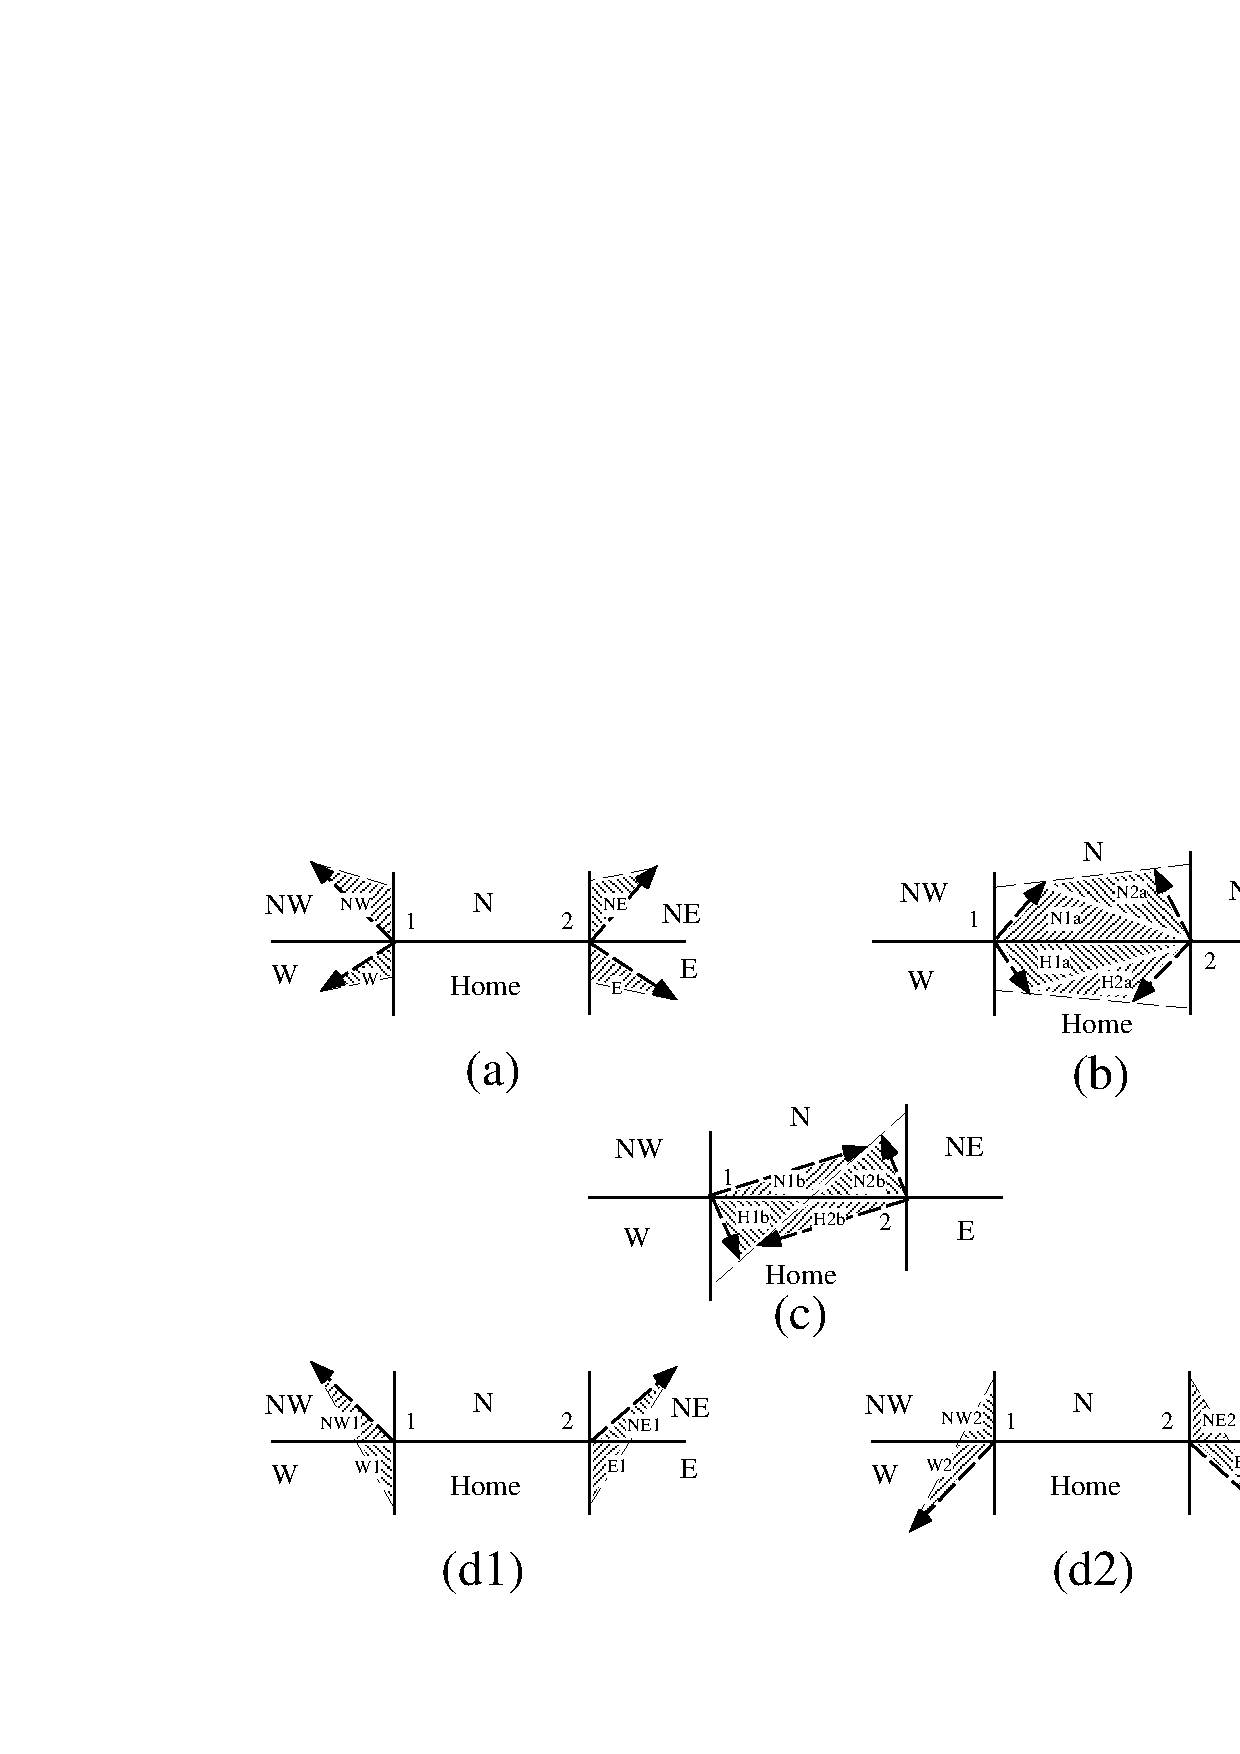
\includegraphics[scale=.7, angle=0, viewport=120 50 800 450,clip]{./Figures/triangles.pdf}
 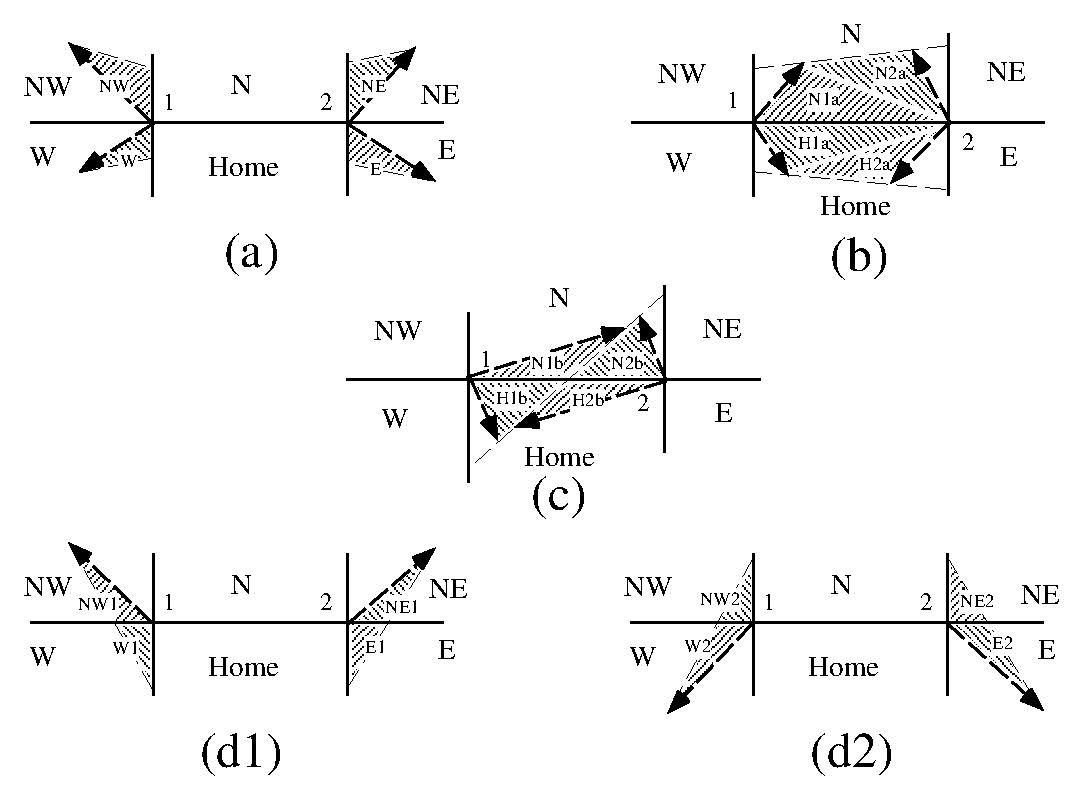
\includegraphics[width=4in]{Figures/triangles.eps}
}
\caption{\label{fig:triangles} The 20 possible triangles that can
contribute fluxes across the north edge of a grid cell.}
\end{figure}


%\newpage
\begin{table}
\begin{center}
\begin{tabular}{cccc}
\hline
Triangle  &  Triangle  &   Selecting logical                   \\
group     &   label    &   condition                           \\
\hline
          &        &            &                                       \\
1         &    NW      &  $y_a>0$ and $y_1\geq0$ and $x_1<0$ \\
          &    NW1     &  $y_a<0$ and $y_1\geq0$ and $x_1<0$ \\
          &    W       &  $y_a<0$ and $y_1<0$ and $x_1<0$    \\
          &    W2      &  $y_a>0$ and $y_1<0$ and $x_1<0$    \\
          &            &                                       \\
2         &    NE      &  $y_b>0$ and $y_2\geq0$ and $x_2>0$    \\
          &    NE1     &  $y_b<0$ and $y_2\geq0$ and $x_2>0$    \\
          &    E       &  $y_b<0$ and $y_2<0$ and $x_2>0$    \\
          &    E2      &  $y_b>0$ and $y_2<0$ and $x_2>0$    \\
          &            &                                       \\
3         &    W1      &  $y_a<0$ and $y_1\geq0$ and $x_1<0$ \\
          &    NW2     &  $y_a>0$ and $y_1<0$ and $x_1<0$    \\
          &    E1      &  $y_b<0$ and $y_2\geq0$ and $x_2>0$ \\
          &    NE2     &  $y_b>0$ and $y_2<0$ and $x_2>0$    \\
          &            &                                       \\
4         &    H1a     &  $y_a y_b\geq 0$ and $y_a+y_b<0$      \\
          &    N1a     &  $y_a y_b\geq 0$ and $y_a+y_b>0$      \\
          &    H1b     &  $y_a y_b<0$ and $\tilde{y}_1<0$      \\
          &    N1b     &  $y_a y_b<0$ and $\tilde{y}_1>0$      \\
          &            &                                       \\
5         &    H2a     &  $y_a y_b\geq 0$ and $y_a+y_b<0$      \\
          &    N2a     &  $y_a y_b\geq 0$ and $y_a+y_b>0$      \\
          &    H2b     &  $y_a y_b<0$ and $\tilde{y}_2<0$      \\
          &    N2b     &  $y_a y_b<0$ and $\tilde{y}_2>0$      \\
          &            &                                       \\
\hline
\end{tabular}
\caption{\label{table:triangles} Evaluation of contributions from the 20 triangles across
the north cell edge.  The coordinates $x_1$, $x_2$, $y_1$, $y_2$,
$y_a$, and $y_b$ are defined in the text. We define $\tilde{y}_1 =
y_1$ if $x_1>0$, else $\tilde{y}_1 = y_a$. Similarly, $\tilde{y}_2
= y_2$ if $x_2<0$, else $\tilde{y}_2 = y_b$.}
\end{center}
\end{table}

\index{grid!horizontal}%
This scheme was originally designed for rectangular grids.  Grid cells in CICE actually lie on the surface of a sphere and must be projected onto a plane.  The projection used in CICE 4.0 maps each grid cell to a square with sides of unit length.  Departure triangles across a given cell edge are computed in a coordinate system whose origin lies at the midpoint of the edge and whose vertices are at (-0.5, 0) and (0.5, 0).  Intersection points are computed assuming Cartesian geometry with cell edges meeting at right angles.  Let CL and CR denote the left and right vertices, which are joined by line CLR.   Similarly, let DL and DR denote the departure points, which are joined by line DLR.  Also, let IL and IR denote the intersection points (0, $y_a$) and (0,$y_b$) respectively, and let IC = ($x_c$, 0) denote the intersection of CLR and DLR.  It can be shown that $y_a$, $y_b$, and $x_c$ are given by
\begin{eqnarray*}
 y_a &=& {x_{CL} (y_{DM}-y_{DL}) + x_{DM}y_{DL} - x_{DL}y_{DM}}\over{x_{DM} - x_{DL}}, \\
 y_b &=& {x_{CR} (y_{DR}-y_{DM}) - x_{DM}y_{DR} + x_{DR}y_{DM}}\over{x_{DR} - x_{DM}}, \\
 x_c &=& x_{DL} - y_{DL} \left({x_{DR} - x_{DL}} \over y_{DR} - y_{DL}\right)
 \end{eqnarray*}
 Each departure triangle is defined by three of the seven points (CL, CR, DL, DR, IL, IR, IC).

Given a 2D velocity field {\bf u},\index{velocity!ice} the divergence $\nabla\cdot{\bf u}$  in a given grid cell can be computed from the local velocities and written in terms of fluxes across each cell edge:
 \begin{equation}
 \label{eq:divergence}
 \nabla\cdot{\bf u} = {1\over A}\left[\left({u_{NE}+u_{SE}}\over 2\right)L_E + \left({u_{NW}+u_{SW}}\over 2\right)L_W + \left({u_{NE}+u_{NW}}\over 2\right)L_N + \left({u_{SE}+u_{SW}}\over 2\right)L_S \right],
 \end{equation}
 where $L$ is an edge length and the indices $N, S, E, W$ denote compass directions.  Equation (\ref{eq:divergence}) is equivalent to the divergence computed in the EVP dynamics (Section~\ref{subsec:dynamics}).  In general, the fluxes in this expression are not equal to those implied by the above scheme for locating departure regions.  For some applications it may be desirable to prescribe the divergence by prescribing the area of the departure region for each edge.  This can be done in CICE 4.0 by setting {\tt l\_fixed\_area} = true in {\bf ice\_transport\_driver.F90} and passing the prescribed departure areas ({\tt edgearea\_e} and {\tt edgearea\_n}) into the remapping routine.  An extra triangle is then constructed for each departure region to ensure that the total area is equal to the prescribed value.  This idea was suggested and first implemented by Mats Bentsen of the Nansen Environmental and Remote Sensing Center (Norway), who applied an earlier version of the CICE remapping scheme to an ocean model.  The implementation in CICE 4.0 is somewhat more general, allowing for departure regions lying on both sides of a cell edge.  The extra triangle is constrained to lie in one but not both of the grid cells that share the edge.  Since this option has yet to be fully tested in CICE, the current default is {\tt l\_fixed\_area} = false.
 
We made one other change in the scheme of \cite{DB:00}  for locating triangles.
In their paper, departure points are defined by projecting cell
corner velocities directly backward.  That is,
\begin{equation}
\label{eq:departure_points} \mathbf{x_D} =
-\mathbf{u} \, \Delta t,
\end{equation}
where $\mathbf{x}_D$ is the location of the departure point
relative to the cell corner and  $\mathbf{u}$ is the velocity at the corner. This approximation is only first-order
accurate. Accuracy can be improved by estimating the 
\index{velocity!ice}%
velocity at the midpoint of the trajectory.

%%%%%%%%%%%%%%%%%%%%%%%%%%%%%%%%%%%%%%%%%%%%%%
\subsubsection{Integrating fields}
\label{subsubsec:integ_flux}


Next, we integrate the reconstructed fields over the departure
triangles to find the total area, volume, and energy transported
across each cell edge.  Area transports are easy to compute since the
area is linear in $x$ and $y$.  Given a triangle with vertices
$\mathbf{x_i} = (x_i,y_i)$, $i\in\{1,2,3\}$, the triangle area is
\begin{equation}
A_T = \frac{1}{2}\left|(x_2-x_1)(y_3-y_1) -
(y_2-y_1)(x_3-x_1)\right|.
\end{equation}
The integral $F_a$ of any linear function $f(\mathbf{r})$ over a
triangle is given by
\begin{equation}
\label{eq:I1}
 F_a = A_T f(\mathbf{x_0}),
\end{equation}
where $\mathbf{x}_0 = (x_0,y_0)$ is the triangle midpoint,
\begin{equation}
\mathbf{x}_0={1\over 3}\sum_{i=1}^3\mathbf{x}_i.
\end{equation}
To compute the area transport, we evaluate the area at the midpoint,
\begin{equation}
a(\mathbf{x}_0)  = a_c + a_x x_0 + a_y y_0,
\end{equation}
and multiply by $A_T$.  By convention, northward and eastward
transport is positive, while southward and westward transport is
negative.

Equation (\ref{eq:I1}) cannot be used for 
\index{volume!ice or snow}%
volume transport, because
the reconstructed volumes are quadratic functions of position.
(They are products of two linear functions, area and thickness.)
The integral of a quadratic polynomial over a triangle requires
function evaluations at three points,
\begin{equation}
\label{eq:I2}
 F_h = \frac{A_T}{3}\sum_{i=1}^3 f\left({\mathbf x}^\prime_i\right),
\end{equation}
where $\mathbf{x}_i^\prime = (\mathbf{x}_0+\mathbf{x}_i)/2$ are
points lying halfway between the midpoint and the three vertices.
\cite{DB:00}  use this formula to compute transports of the product $\rho \, T$,
which is analogous to ice volume.  Equation (\ref{eq:I2}) does not
work for ice and snow energies, which are cubic
functions---products of area, thickness, and enthalpy. Integrals
of a cubic polynomial over a triangle can be evaluated using a
four-point formula \cite{Stroud:71}:
\begin{equation}
\label{eq:I3}
 F_q = A_T \left[ -\frac{9}{16} f(\mathbf{x}_0) +
              \frac{25}{48} \sum_{i=1}^3 f(\mathbf{x}_i^{\prime\prime})\right]
\end{equation}
where $\mathbf{x_i}^{\prime\prime}=(3 \mathbf{x}_0 + 2
\mathbf{x}_i)/5$.
To evaluate functions at specific points,
we must compute many products of the form
$a({\bf x}) \, h({\bf x})$ and
$a({\bf x}) \, h({\bf x}) \, q({\bf x})$,
where each term in the product is the sum of a cell-center value
and two displacement terms.  In the code, the computation is sped up by
storing some sums that are used repeatedly.

%%%%%%%%%%%%%%%%%%%%%%%%%%%%%%%%%%%%%%%%%%%%%%
\subsubsection{Updating state variables}
\label{subsubsec:update_state}
\index{state variables|(}%

Finally, we compute new values of the state variables
in each ice category and grid cell.
The new 
\index{ice!fraction}%
fractional ice areas $a_{in}^\prime(i,j)$ are given by
\begin{equation}
\label{eq:new_area}
a_{in}^\prime(i,j) = a_{in}(i,j) +
              \frac{F_{aE}(i-1,j) - F_{aE}(i,j)
                  + F_{aN}(i,j-1) - F_{aN}(i,j)}
                   {A(i,j)}
\end{equation}
where $F_{aE}(i,j)$ and $F_{aN}(i,j)$ are the area transports across the
east and north edges, respectively, of cell $(i,j)$, and $A(i,j)$
is the grid cell area.   All transports added to one cell are
subtracted from a neighboring cell; thus (\ref{eq:new_area})
conserves total ice area.\index{conservation}

The new ice 
\index{volume!ice or snow}%
volumes and energies are computed analogously.
New 
\index{thickness!ice or snow}%
thicknesses are given by the ratio of volume to area,
and enthalpies by the ratio of energy to volume.
Tracer 
\index{monotonicity}%
monotonicity is ensured because
\[ h^\prime = {\int_A a \, h \, dA \over \int_A a \, dA}, \]
\[ q^\prime  = {\int_A a \, h \, q\,dA \over \int_A a \, h \ dA}, \]
where $h^\prime$ and $q^\prime$ are the new-time thickness\index{thickness!ice or snow} and
enthalpy,\index{enthalpy} given by integrating the old-time ice area, volume, and
energy over a Lagrangian departure region with area $A$. That is,
the new-time thickness and enthalpy are weighted averages over
old-time values, with non-negative weights $a$ and $ah$. Thus the
new-time values must lie between the maximum and minimum of the
old-time values.
\index{state variables|)}
\index{transport!horizontal|)}

%%%%%%%%%%%%%%%%%%%%%%%%%%%%%%%%%%%%%%%%%%%%%%
\subsection{Transport in thickness space}
\markboth{Model components}{Transport in thickness space}
\label{subsec:itd_transport}
\index{boundary!thickness category|(emph}
\index{transport!thickness|(emph}
\index{thickness!distribution|(emph}

Next we solve the equation for ice transport in thickness space due to
thermodynamic 
\index{ice!growth}%
growth and melt,
\begin{equation}
\label{eq:itd_transport}
\frac{\partial g}{\partial t} + \frac{\partial}{\partial h} (f g) = 0,
\end{equation}
which is obtained from (\ref{eq:transport_g}) by neglecting the
first and third terms on the right-hand side. We use the remapping
method of \cite{Lipscomb:01}, in which thickness categories are
represented as Lagrangian grid cells whose boundaries are
projected forward in time. The thickness distribution function $g$
is approximated as a linear function of $h$ in each displaced
category and is then remapped onto the original thickness
categories. This method is numerically smooth  and is not too
diffusive. It can be viewed as a 1D simplification of the 2D
incremental remapping scheme described above.

We first compute the displacement of category boundaries in thickness
space.  Assume that at time $m$ the 
\index{ice!fraction}%
ice areas $a_n^m$
and mean ice thicknesses $h_n^m$ are known for each thickness category.
(For now we omit the subscript $i$ that distinguishes ice from snow.)
We use a thermodynamic model
(Section~\ref{subsec:thermo}) to compute the new mean thicknesses
$h_n^{m+1}$ at time $m+1$.  The time step 
\index{CFL condition}%
must be small enough that
trajectories do not cross; i.e., $h_n^{m+1} < h_{n+1}^{m+1}$ for each
pair of adjacent categories.  The 
\index{ice!growth}%
growth rate at $h = h_n$ is given
by $f_n = (h_n^{m+1} - h_n^m) / \Delta t$.  By linear interpolation
we estimate the growth rate $F_n$ at the upper category boundary $H_n$:
\[ F_n = f_n + \frac{f_{n+1}-f_n}{h_{n+1}-h_n} \, (H_n - h_n). \]
If $a_n$ or $a_{n+1} = 0$, $F_n$ is set to the growth rate in the
nonzero category, and if $a_n = a_{n+1} = 0$, we set $F_n = 0$.
The temporary displaced boundaries are given by
\[ H_n^* = H_n + F_n \, \Delta t, \ n = 1 \ {\rm to} \ N-1  \]
The boundaries must not be displaced by more than one category
to the left or right; that is, we require $H_{n-1} < H_n^* < H_{n+1}$.
Without this requirement we would need to do a general remapping
rather than an incremental remapping, at the cost of added
complexity.

Next we construct $g(h)$ in the displaced thickness
categories.  The 
\index{ice!fraction}%
ice areas in the displaced categories are
$a_n^{m+1} = a_n^m$, since
area is conserved\index{conservation} following the motion in thickness space (i.e., during
vertical ice growth or melting).   The new ice 
\index{volume!ice or snow}%
volumes are
$v_n^{m+1} = (a_n h_n)^{m+1} = a_n^m h_n^{m+1}$.
For conciseness, define
$H_L = H_{n-1}^*$ and $H_R = H_{n}^*$ and drop the time index $m+1$.
We wish to construct
a continuous function $g(h)$ within each category such that the total
area and volume at time $m+1$ are $a_n$ and $v_n$, respectively:
\begin{equation}
\label{eq:area_cons}
\int_{H_L}^{H_R} g \, dh = a_n,
\end{equation}
\begin{equation}
\label{eq:volume_cons}
\int_{H_L}^{H_R} h \, g \, dh = v_n.
\end{equation}
The simplest polynomial that can satisfy both equations is a line.
It is convenient to change coordinates, writing
$g(\eta) = g_1 \eta + g_0$, where $\eta = h - H_L$ and the
coefficients $g_0$ and $g_1$ are to be determined.  Then
(\ref{eq:area_cons}) and (\ref{eq:volume_cons}) can be written as
\[ g_1 \frac{\eta_R^2}{2} + g_0 \eta_R = a_n, \]
\[ g_1 \frac{\eta_R^3}{3} + g_0 \frac{\eta_R^2}{2} = a_n \eta_n, \]
where $\eta_R = H_R - H_L$ and $\eta_n = h_n - H_L$.
These equations have the solution
\begin{equation}
\label{eq:g0}
g_0 = \frac{6 a_n}{\eta_R^2} \left(\frac{2 \eta_R}{3} - \eta_n\right),
\end{equation}
\begin{equation}
\label{eq:g1}
g_1 = \frac{12 a_n}{\eta_R^3} \left(\eta_n - \frac{\eta_R}{2}\right).
\end{equation}

Since $g$ is linear, its maximum and minimum values lie at
the boundaries, $\eta = 0$ and $\eta_R$:
\begin{equation}
\label{eq:gmin}
g(0)=\frac{6 a_n}{\eta_R^2} \, \left(\frac{2 \eta_R}{3} - \eta_n\right) = g_0,
\end{equation}
\begin{equation}
\label{eq:gmax}
g(\eta_R) = \frac{6 a_n}{\eta_R^2} \, \left(\eta_n - \frac{\eta_R}{3}\right).
\end{equation}
Equation (\ref{eq:gmin}) implies that $g(0) < 0$ when $\eta_n > 2 \eta_R/3$,
i.e., when $h_n$ lies in the right third of the thickness range $(H_L, H_R)$.
Similarly, (\ref{eq:gmax}) implies that $g(\eta_R) < 0$ when
$\eta_n < \eta_R/3$, i.e.,
when $h_n$ is in the left third of the range.  Since negative values
of $g$ are unphysical, a different solution is needed when $h_n$ lies
outside the central third of the thickness range.  If $h_n$ is in
the left third of the range, we define a cutoff thickness,
$H_C = 3 h_n - 2 H_L$, and set $g = 0$ between $H_C$ and $H_R$.
Equations (\ref{eq:g0}) and (\ref{eq:g1}) are then valid
with $\eta_R$ redefined as $H_C - H_L$.  And if $h_n$ is
in the right third of the range, we define $H_C = 3 h_n - 2 H_R$ and
set $g = 0$ between $H_L$ and $H_C$.  In this case, (\ref{eq:g0}) and
(\ref{eq:g1}) apply with $\eta_R = H_R - H_C$ and $\eta_n = h_n - H_C$.

Figure~\ref{fig:gplot} illustrates the linear reconstruction of $g$
for the simple cases $H_L = 0$, $H_R = 1$, $a_n = 1$, and $h_n =$
0.2, 0.4, 0.6, and 0.8.  Note that $g$ slopes downward ($g_1 < 0$)
when $h_n$ is less than the midpoint thickness, $(H_L + H_R)/2 = 1/2$,
and upward when $h_n$ exceeds the midpoint thickness.
For $h_n = 0.2$ and 0.8, $g = 0$ over part of the range.

\begin{figure}
\centerline{
\includegraphics[scale=.4, viewport=80 50 700 550,clip]{./Figures/gplot.pdf}
}
\caption{\label{fig:gplot} Linear approximation of the thickness
distribution function $g(h)$ for an ice category with left boundary
$H_L = 0$, right boundary $H_R = 1$, fractional area $a_n = 1$, and
mean ice thickness $h_n = $ 0.2, 0.4, 0.6, and 0.8.}
\end{figure}

Finally, we remap the thickness distribution to the original
boundaries by transferring area and volume\index{volume!ice or snow} between categories.
We compute the 
\index{ice!fraction}%
ice area
$\Delta a_n$ and 
\index{volume!ice or snow}%
volume $\Delta v_n$ between each original boundary
$H_n$ and displaced boundary $H_n^*$.  If $H_n^* > H_n$, ice
moves from category $n$ to $n+1$.  The area and volume transferred are
\begin{equation}
\label{eq:move_area}
\Delta a_n = \int_{H_n}^{H_n^*} g \, dh,
\end{equation}
\begin{equation}
\label{eq:move_volume}
\Delta v_n = \int_{H_n}^{H_n^*} h \, g \, dh.
\end{equation}
If $H_n^* < H_N$, ice area and volume are transferred
from category $n+1$ to $n$ using (\ref{eq:move_area}) and
(\ref{eq:move_volume}) with the limits of integration reversed.
To evaluate the integrals we change coordinates from $h$ to
$\eta = h - H_L$, where $H_L$ is the left limit of the range
over which $g > 0$, and write $g(\eta)$ using
(\ref{eq:g0}) and (\ref{eq:g1}).
In this way we obtain the new areas $a_n$ and volumes $v_n$ between
the original boundaries $H_{n-1}$ and $H_n$ in each category.
The new thicknesses, $h_n = v_n/a_n$, are guaranteed to lie
in the range $(H_{n-1}, H_n)$.  If $g = 0$ in the part of a category
that is remapped to a neighboring category, no ice is transferred.

Other conserved quantities are transferred in proportion to the ice
volume $\Delta v_{in}$.  
%(We now use the subscripts $i$ and $s$ to distinguish ice from snow.)  
For example,
the transferred 
%snow volume is
%$\Delta v_{sn} = v_{sn} (\Delta v_{in} / v_{in})$,
%and the transferred 
ice energy in layer $k$ is
$\Delta e_{ink} = e_{ink} (\Delta v_{in} / v_{in})$.

The left and right boundaries of the domain require special treatment.
If ice is growing\index{ice!growth} in 
\index{open water|(emph}%
open water at a rate $F_0$, the left boundary
$H_0$ is shifted to the right by $F_0 \Delta t$ before $g$ is
constructed in category 1, then reset to zero after the remapping
is complete.  New ice is then added to the grid cell, 
\index{conservation}%
conserving
area, volume, and energy.  If ice cannot grow in open water (because
the ocean is too warm or the net surface energy flux is downward),
$H_0$ is fixed at zero, and the growth rate at the left boundary
is estimated as $F_0 = f_1$.  If $F_0 < 0$, all ice thinner than
$\Delta h_0 = -F_0 \Delta t$ is assumed to have melted, and the ice area in category 1 is reduced accordingly.   The area
of new open water is
\[ \Delta a_0 = \int_{0}^{\Delta h_0} g \, dh. \]
The right boundary $H_N$ is not fixed but varies with $h_N$, the
mean ice thickness in the thickest category.  Given $h_N$, we set
$H_N = 3 h_N - 2 H_{N-1}$, which ensures that $g(h) > 0$ for
$H_{N-1} < h < H_N$ and $g(h) = 0$ for $h \geq H_N$. No ice
crosses the right boundary.
\index{open water|)}%

\index{ice!growth}%
If the ice growth or melt rates in a given grid cell are too
large, the thickness remapping scheme will not work.  Instead, the
thickness categories in that grid cell are treated as delta
functions following \cite{BHWE:01}, and categories outside their
prescribed boundaries are merged with neighboring categories as
needed. For time steps of less than a day and category thickness
ranges of 10 cm or more, this simplification is needed rarely, if
ever.

\index{monotonicity}
The linear remapping algorithm for thickness is not monotonic for tracers, although significant errors rarely occur.  Usually they appear as snow temperatures\index{temperature!ice or snow} (enthalpy)\index{enthalpy} outside the physical range of values in very small snow volumes.\index{volume!ice or snow}\index{thickness!ice or snow}   In this case we transfer the snow and its heat\index{ocean!heat} and tracer\index{tracers} contents to the ocean.
\index{boundary!thickness category|)}
\index{transport!thickness|)}%
%\index{transport|)}%
\index{remapping!incremental|)}%

%%%%%%%%%%%%%%%%%%%%%%%%%%%%%%%%%%%%%%%%%%%%%%
\subsection{Mechanical redistribution}
\markboth{Model components}{Mechanical redistribution}
\label{subsec:mech_red}
\index{ridging|(emph}
\index{ice!fraction|(}
The last term on the right-hand side of (\ref{eq:transport_g}) is $\psi$, which describes the redistribution of ice in thickness space due to ridging and other mechanical processes. The mechanical redistribution scheme in CICE is based on \cite{TRMC:75}, \cite{Rothridge:75}, \cite{Hib:80}, \cite{FH:95}, and \cite{LHMJ:07}.  This scheme converts thinner ice to thicker ice and is applied after horizontal transport.  When the ice is converging, enough ice ridges to ensure that the ice 
\index{ice!fraction}%
area does not exceed the grid cell area.

First we specify the participation function: the thickness distribution $a_P(h) = b(h) \, g(h)$ of the ice participating in ridging.  (We use ``ridging'' as shorthand for all forms of mechanical redistribution, including rafting.) The weighting function $b(h)$ favors ridging of thin ice and closing of 
%\index{open water}%
open water in preference to ridging of thicker ice.  There are two options for the form of $b(h)$.  If {\tt krdg\_partic} = 0 in the namelist,\index{namelist} we follow \cite{TRMC:75} and set 
\begin{equation}
\label{eq:partic_old_contin}
b(h) = \left\{\begin{array}{ll}  
       \frac{2}{G^*}(1-\frac{G(h)}{G^*}) & \mbox{if $G(h)<G^*$} \\
                 0                       & \mbox{otherwise}   
              \end{array}  \right.
\end{equation}
where $G(h)$ is the fractional area covered by ice thinner than $h$, and $G^*$ is an empirical constant.  Integrating $a_P(h)$ between category boundaries $H_{n-1}$ and $H_n$, we obtain the mean value of $a_P$ in category $n$: 
\begin{equation}
\label{eq:partic_old_discrete}
a_{Pn} = \frac{2}{G^*} (G_n - G_{n-1})
         \left( 1 - \frac{G_{n-1}+G_n}{2 G^*} \right),
\end{equation}
where $a_{Pn}$ is the ratio of the ice area ridging (or open water area closing) in category $n$ to the total area ridging and closing, and $G_n$ is the total fractional ice area in categories 0 to $n$. Equation~(\ref{eq:partic_old_discrete}) applies to categories with $G_n < G^*$.  If $G_{n-1} < G^* < G_n$, then (\ref{eq:partic_old_discrete}) is valid with $G^*$ replacing $G_n$, and if $G_{n-1} > G^*$, then $a_{Pn} = 0$.  If the 
\index{open water}%
open water fraction $a_0 > G^*$, no ice can ridge, because ``ridging'' simply reduces the area of open water.  As in \cite{TRMC:75} we set $G^* = 0.15$.

\index{stability}%
If the spatial resolution is too fine for a given time step $\Delta t$, the weighting function 
(\ref{eq:partic_old_contin}) can promote numerical instability.  For $\Delta t = \mbox{1 hour}$, resolutions finer than $\Delta x \sim \mbox{10 km}$ are typically unstable.  The instability results from feedback between the ridging scheme and the dynamics via the ice strength.\index{strength}  If the strength changes significantly on time scales less than $\Delta t$, the viscous-plastic solution of the momentum equation\index{momentum equation} is inaccurate and sometimes oscillatory.  As a result, the fields of ice area, thickness, velocity, strength, divergence, and shear can become noisy and unphysical. 

A more stable weighting function was suggested by \cite{LHMJ:07}:
%lipscomb - eqn. 57 from paper
\begin{equation}
\label{eq:partic_new_contin}
b(h) = \frac{\exp[-G(h)/a^*]}
            {a^*[1-\exp(-1/a^*)]}
\end{equation}
When integrated between category boundaries, (\ref{eq:partic_new_contin}) implies
%lipscomb - eqn. 58 from paper
\begin{equation}
\label{eq:partic_new_discrete}
a_{Pn} = \frac {\exp(-G_{n-1}/a^*) - \exp(-G_{n}/a^*)}
               {1 - \exp(-1/a^*)}
\end{equation}
This weighting function is used if {\tt krdg\_partic} = 1 in the namelist.\index{namelist}  From (\ref{eq:partic_new_contin}), the mean value of $G$ for ice participating in ridging is $a^*$, as compared to $G^*/3$ for (\ref{eq:partic_old_contin}).  For typical ice thickness distributions, setting $a^* = 0.05$ with {\tt krdg\_partic} = 1 gives participation fractions similar to those given by $G^* = 0.15$ with {\tt krdg\_partic} = 0.  See \cite{LHMJ:07} for a detailed comparison of these two participation functions.
 
Thin ice is converted to thick, ridged ice in a way that reduces the total 
ice area while 
\index{conservation}\index{volume!ice or snow}%
conserving ice volume and internal energy.  There are two namelist options for redistributing ice among thickness categories.  If {\tt krdg\_redist} = 0, ridging ice of thickness $h_n$ forms ridges whose area is distributed uniformly between $H_{\min} = 2 h_n$ and $H_{\max} = 2 \sqrt{H^* h_n}$, as in \cite{Hib:80}. The default value of $H^*$ is 25~m, as in earlier versions of CICE.  Observations suggest that $H^* = 50$~m gives a better fit to first-year ridges \cite{AMI:04}, although the lower value may be appropriate for multiyear ridges \cite{FH:95}.  The ratio of the mean ridge thickness to the thickness of ridging ice is $k_n = (H_{\min} + H_{\max}) / (2 h_n)$. If the area of category $n$ is reduced by ridging at the rate $r_n$, the area of thicker categories grows simultaneously at the rate $r_n/k_n$.  Thus the \emph{net} rate of area loss due to ridging of ice in category $n$ is $r_n(1-1/k_n)$.  

The ridged ice area and 
\index{volume!ice or snow}%
volume are apportioned among categories in the thickness range $(H_{\min}, H_{\max})$.  The fraction of the new ridge area in category $m$ is
\begin{equation}
\label{eq:ridge_area_old}
f_m^{\mathrm{area}} = \frac{H_R - H_L} 
                           {H_{\max} - H_{\min}},
\end{equation}
where $H_L = \max(H_{m-1},H_{\min})$ and $H_R= \min(H_m,H_{\max})$. The fraction of the ridge volume going to category $m$ is
\begin{equation}
\label{eq:ridge_volume_old}
f_m^{\mathrm{vol}} = \frac{(H_R)^2 - (H_L)^2}
                          {(H_{\max})^2 - (H_{\min})^2}.
\end{equation}

This uniform redistribution function tends to produce too little ice in the 3--5~m range and too much ice thicker than 10~m \cite{AMI:04}.  Observations show that the ITD of ridges is better approximated by a negative exponential.  Setting {\tt krdg\_redist} = 1 gives ridges with an exponential ITD \cite{LHMJ:07}:
\begin{equation}
\label{eq:redist_new}
g_R(h) \propto \exp[-(h - H_{\min})/\lambda]
\end{equation}
for $h \ge H_{\min}$, with $g_R(h) = 0$ for $h < H_{\min}$.  Here, $\lambda$ is an empirical {\it e}-folding scale and $H_{\min}=2h_n$ (where $h_n$ is the thickness of ridging ice).  We assume that $\lambda = \mu h_n^{1/2}$, where $\mu$ ({\tt mu\_rdg}) is a tunable parameter with units \mbox{m$^{1/2}$}.  Thus the mean ridge thickness increases in proportion to $h_n^{1/2}$, as in \cite{Hib:80}.  The value $\mu = 4.0$~\mbox{m$^{1/2}$} gives $\lambda$ in the range 1--4 m for most ridged ice.  Ice strengths\index{strength} with $\mu = 4.0$~\mbox{m$^{1/2}$} and {\tt krdg\_redist} = 1 are roughly comparable to the strengths with $H^* = 50$~m and {\tt krdg\_redist} = 0.
 
From (\ref{eq:redist_new}) it can be shown that the fractional area going to category $m$ as a result of ridging is
\begin{equation}
\label{eq:ridge_area_new}
f_m^{\mathrm{area}} = \exp[-(H_{m-1} - H_{\min}) / \lambda] 
                     - \exp[-(H_m - H_{\min}) / \lambda].
\end{equation}
The fractional volume going to category $m$ is
\begin{equation}
\label{eq:ridge_volume_new}
f_m^{\mathrm{vol}} = \frac{(H_{m-1}+\lambda) \exp[-(H_{m-1}-H_{\min})/\lambda]
                           - (H_m + \lambda) \exp[-(H_m - H_{\min}) / \lambda]}
                             {H_{min} + \lambda}.
\end{equation}
Equations (\ref{eq:ridge_area_new}) and (\ref{eq:ridge_volume_new}) replace (\ref{eq:ridge_area_old}) and (\ref{eq:ridge_volume_old}) when {\tt krdg\_redist} = 1.

Internal ice energy is transferred between categories in proportion to ice volume.  
\index{volume!ice or snow}%
Snow volume and internal energy are transferred in the same way, except that a fraction of the snow may be deposited in the ocean instead of added to the new ridge.\index{fresh water flux}  

The net area removed by ridging and closing is a function of the strain rates.\index{strain rate}  Let $R_{\mathrm{net}}$ be the net rate of area loss for the ice pack (i.e., the rate of 
\index{open water}%
open water area closing, plus the net rate of ice area loss due to ridging).  Following \cite{FH:95}, $R_{\mathrm{net}}$ is given by
\begin{equation}
\label{eq:Rnet}
R_{\mathrm{net}} = \frac{C_s}{2}
                 (\Delta - |D_D|) - \min(D_D,0),
\end{equation}
where $C_s$ is the fraction of shear dissipation energy that 
contributes to ridge-building, $D_D$ is the divergence, and $\Delta$ is a function of 
\index{strain rate}%
the divergence and shear.  These strain rates are computed by the
%\index{elastic!-viscous-plastic dynamics}% 
dynamics scheme.  The default value of $C_s$ is 0.25.

Next, define $R_{\mathrm{tot}} = \sum_{n=0}^N r_n$.  This rate is related to $R_{\mathrm{net}}$ by
\begin{equation}
\label{eq:Rtot_Rnet}
R_{\mathrm{net}} =
   \left[ a_{P0} + \sum_{n=1}^N a_{Pn}\left(1-{1\over k_n}\right)\right]
    R_{\mathrm{tot}}.
\end{equation}
Given $R_{\mathrm{net}}$ from~(\ref{eq:Rnet}), we use~(\ref{eq:Rtot_Rnet}) to compute $R_{\mathrm{tot}}$. Then the area ridged in category $n$ is given by $a_{rn} = r_n \Delta t$, where $r_n = a_{Pn} R_{\mathrm{tot}}$. The area of new ridges is $a_{rn} / k_n$, and the 
\index{volume!ice or snow}%
volume of new ridges is $a_{rn} h_n$ (since volume is conserved\index{conservation} during ridging).  We remove the ridging ice from category $n$ and use~(\ref{eq:ridge_area_old}) and~(\ref{eq:ridge_volume_old}) (or \ref{eq:ridge_area_new}) and (\ref{eq:ridge_volume_new})) to redistribute the ice among thicker categories.

Occasionally the ridging rate in thickness category $n$ may be large enough to ridge the entire area $a_n$ during a time interval less than $\Delta t$.  In this case $R_{\mathrm{tot}}$ is reduced to the value that exactly ridges an area $a_n$ during $\Delta t$. After each ridging iteration, the total 
fractional ice area $a_i$ is computed.  If $a_i > 1$, the ridging is repeated with a value of $R_{\mathrm{net}}$ sufficient to yield $a_i = 1$.

\index{ice!level|emph} \index{tracers}
Two tracers for tracking the ridged ice area and volume\index{volume!ice or snow} are available.  The 
actual tracers are for level (undeformed) ice area ({\tt alvl}) and volume ({\tt vlvl}), 
which are easier to implement for a couple of reasons: (1) ice ridged in a given 
thickness category is spread out among the rest of the categories, making it 
more difficult (and expensive) to track than the level ice remaining behind 
in the original category; (2)  previously ridged ice may ridge again, so that 
simply adding a volume of freshly ridged ice to the volume of previously 
ridged ice in a grid cell may be inappropriate.   Although the code currently 
only tracks level ice internally, both level ice and ridged ice are offered 
as history\index{history} output.  They are simply related:
\begin{eqnarray*}
a_{lvl} + a_{rdg} &=& a_i, \\
v_{lvl} + v_{rdg} &=& v_i.
\end{eqnarray*}
Level ice area fraction and volume increase with new ice formation and 
decrease steadily via ridging processes.  Without the formation of new ice, 
level ice asymptotes to zero because we assume that both level ice and ridged 
ice ridge, in proportion to their fractional areas in a grid cell (in the 
spirit of the ridging calculation itself which does not prefer level ice over 
previously ridged ice). 

The ice 
\index{strength|(}%
strength $P$ may be computed in either of two ways.  If the namelist\index{namelist} parameter {\tt kstrength} = 0, we use the strength formula from \cite{Hib:79}:
\begin{equation}
\label{eq:hib_strength} 
P = P^* h \exp[-C(1-a_i)],
\end{equation}
where $P^* = 27,500 \, \mathrm {N/m}$ and $C = 20$ are empirical constants, and $h$ is the mean ice thickness. Alternatively, setting {\tt kstrength} = 1 gives an ice strength closely related to the ridging scheme. Following \cite{Rothridge:75}, the strength is assumed proportional to the change in ice potential energy $\Delta E_P$ per unit area of compressive deformation. Given uniform ridge ITDs ({\tt krdg\_redist} = 0), we have
\begin{equation}
\label{eq:roth_strength0} 
P = C_f \, C_p \, \beta \sum_{n=1}^{N_C}
  \left[ -a_{Pn} \, h_n^2  + \frac{a_{Pn}}{k_n}
     \left( \frac{(H_n^{\max})^3 - (H_n^{\min})^3}
                 {3(H_n^{\max}-H_n^{\min})} \right) \right],
\end{equation}
where $C_P = (g/2)(\rho_i/\rho_w)(\rho_w-\rho_i)$, $\beta =R_{\mathrm{tot}}/R_{\mathrm{net}} > 1$ from~(\ref{eq:Rtot_Rnet}), and $C_f$ is an empirical parameter that accounts for frictional energy dissipation. Following \cite{FH:95}, we set $C_f = 17$. The first term in the summation is the potential energy of ridging ice, and the second, larger term is the potential energy of the resulting ridges.  The factor of $\beta$ is included because $a_{Pn}$ is normalized with respect to the total area of ice ridging, not the net area removed.  Recall that more than one unit area of ice must be ridged to reduce the net ice area by one unit.  For exponential ridge ITDs ({\tt krdg\_redist} = 1), the ridge potential energy is modified:
\begin{equation}
\label{eq:roth_strength1} 
P = C_f \, C_p \, \beta \sum_{n=1}^{N_C}
  \left[ -a_{Pn} \, h_n^2  + \frac{a_{Pn}}{k_n}
     \left( H_{\min}^2 + 2H_{\min}\lambda + 2 \lambda^2 \right) \right]  % CHECK BRACES
\end{equation}

The energy-based ice strength given by (\ref{eq:roth_strength0}) or (\ref{eq:roth_strength1}) is more physically realistic than the strength given by (\ref{eq:hib_strength}).  However, use of (\ref{eq:hib_strength}) is less likely to allow numerical instability at a given resolution and time step.  See \cite{LHMJ:07} for more details.
\index{strength|)}%
\index{ridging|)}%
\index{ice!fraction|)}
\index{thickness!distribution|)}

%%%%%%%%%%%%%%%%%%%%%%%%%%%%%%%%%%%%%%%%%%%%%%
\subsection{Dynamics}
\markboth{Model components}{Dynamics}
\label{subsec:dynamics}
\index{elastic!-viscous-plastic dynamics|(emph}
\index{velocity!ice|(emph}
\index{internal stress|(emph}

There are now different rheologies available in the CICE code. The elastic-viscous-plastic (EVP) model represents a modification of the standard viscous-plastic (VP) model for sea ice dynamics \cite{Hib:79}.  The elastic-anisotropic-plastic (EAP) model,\index{elastic!-anisotropic-plastic dynamics} 
on the other hand, explicitly accounts for the observed sub-continuum anisotropy of the sea ice cover \cite{WF:06,WS:09}. If {\tt kdyn}~=~1 in the namelist\index{namelist} then the EVP rheology is used (module {\bf ice\_dyn\_evp.F90}), while {\tt kdyn}~=~2 is associated with the EAP rheology ({\bf ice\_dyn\_eap.F90}).  At times scales associated with the wind forcing, the EVP model reduces to the VP model while the EAP model reduces to the anisotropic rheology described in detail in \cite{WF:06,Tsamados:13}. At shorter time scales the adjustment process takes place in both models by a numerically more efficient \index{elastic!waves}%
elastic wave
mechanism.
While retaining the essential physics, this elastic wave
modification leads to a fully explicit numerical scheme which greatly
improves the model's computational efficiency.

The EVP sea ice dynamics model is
thoroughly documented in \cite{HD:97}, \cite{ech_JCP:01}, \cite{HD:02} and \cite{HD:03} and the EAP dynamics in \cite{Tsamados:13}.
Simulation results and performance of the EVP and EAP models have been compared with the VP model and with each other in realistic simulations of the Arctic respectively in \cite{HZ:99} and \cite{Tsamados:13}.
Here we summarize the equations and direct the
reader to the above references for details.  The numerical implementation in this code
release is that of \cite{HD:02} and \cite{HD:03}, with revisions to the numerical solver as in \cite{BFLM:13}.  The implementation of the EAP sea ice dynamics into CICE is described in detail in \cite{Tsamados:13}.

\subsubsection{Momentum}
\label{subsec:momentum}

The force balance per unit area in the ice pack is given by a two-dimensional
\index{momentum equation|(emph}%
momentum equation \cite{Hib:79}, obtained by integrating the 3D equation
through the 
\index{thickness!ice or snow}
thickness of the ice in the vertical direction:
\begin{equation}
\label{eq:vpmom}
m{\partial {\bf u}\over\partial t} = \nabla\cdot{\bf \sigma}
+ \vec{\tau}_a+\vec{\tau}_w - \hat{k}\times mf{\bf u} - mg\nabla H_\circ,
\end{equation}
where $m$ is the combined mass of ice and 
\index{volume!ice or snow}%
snow per unit area and 
$\vec{\tau}_a$ and
$\vec{\tau}_w$ are 
\index{wind!stress}%
wind and 
\index{ice--ocean stress}%
ocean stresses,
respectively. The 
%\index{strength}%
strength of the ice is represented by the internal
stress tensor $\sigma_{ij}$, and the other two terms on the right hand
side are stresses due to 
\index{Coriolis}%
Coriolis effects and the sea surface
\index{slope, sea surface}%
slope.   The parameterization for  the wind and ice--ocean stress terms must contain the ice concentration as a multiplicative factor to be 
consistent with the formal theory of free drift in low ice concentration regions.    A careful explanation of the issue and its continuum solution is provided in \cite{HD:03} and \cite{CGHM:04}.

The momentum equation is discretized in time as follows, for the classic EVP approach.  First, for clarity, the two components of (\ref{eq:vpmom}) are
\begin{eqnarray*}
m{\partial u\over\partial t} &=& {\partial\sigma_{1j}\over\partial x_j} + \tau_{ax} + 
  a_i c_w \rho_w
  \left|{\bf U}_w - {\bf u}\right| \left[\left(U_w-u\right)\cos\theta - \left(V_w-v\right)\sin\theta\right]
  +mfv - mg{\partial H_\circ\over\partial x}, \\
m{\partial v\over\partial t} &=& {\partial\sigma_{2j}\over\partial x_j} + \tau_{ay} + 
  a_i c_w \rho_w
  \left|{\bf U}_w - {\bf u}\right| \left[\left(U_w-u\right)\sin\theta - \left(V_w-v\right)\cos\theta\right]
  -mfu - mg{\partial H_\circ\over\partial y}. 
\end{eqnarray*}
In the code, ${\tt vrel}=a_i c_w \rho_w\left|{\bf U}_w - {\bf u}^k\right|$, where $k$ denotes the subcycling step.\index{subcycling}  The following equations illustrate the time discretization and define some of the other variables used in the code.
\small
\begin{equation}
\label{eq:umom}
\underbrace{\left({m\over\Delta t_e}+{\tt vrel} \cos\theta\right)}_{\tt cca} u^{k+1} 
- \underbrace{\left(mf+{\tt vrel}\sin\theta\right)}_{\tt ccb}v^{k+1}
 =  \underbrace{{\partial\sigma_{1j}^{k+1}\over\partial x_j}}_{\tt strintx} 
 + \underbrace{\tau_{ax} - mg{\partial H_\circ\over\partial x} }_{\tt forcex}
  + {\tt vrel}\underbrace{\left(U_w\cos\theta-V_w\sin\theta\right)}_{\tt waterx}  + {m\over\Delta t_e}u^k,
\end{equation}
\begin{equation}
\label{eq:vmom}
 \underbrace{\left(mf+{\tt vrel}\sin\theta\right)}_{\tt ccb} u^{k+1} 
+ \underbrace{\left({m\over\Delta t_e}+{\tt vrel} \cos\theta\right)}_{\tt cca}v^{k+1}
 =  \underbrace{{\partial\sigma_{2j}^{k+1}\over\partial x_j}}_{\tt strinty} 
 + \underbrace{\tau_{ay} - mg{\partial H_\circ\over\partial y} }_{\tt forcey}
  + {\tt vrel}\underbrace{\left(U_w\sin\theta+V_w\cos\theta\right)}_{\tt watery}  + {m\over\Delta t_e}v^k,
\end{equation}
\normalsize
and {\tt vrel$\cdot$waterx(y) = taux(y)}.  

We solve this system of equations analytically for $u^{k+1}$ and $v^{k+1}$.   Define
\begin{eqnarray}
\label{eq:cevpuhat}
\hat{u} &=& F_u + \tau_{ax} - mg{\partial H_\circ\over\partial x} + {\tt vrel} \left(U_w\cos\theta - V_w\sin\theta\right) + {m\over\Delta t_e}u^k \\
\label{eq:cevpvhat}
\hat{v} &=& F_v + \tau_{ay} - mg{\partial H_\circ\over\partial y} + {\tt vrel} \left(U_w\sin\theta + V_w\cos\theta\right) + {m\over\Delta t_e}v^k, 
\end{eqnarray}
where ${\bf F} = \nabla\cdot\sigma^{k+1}$.  Then
\begin{eqnarray*}
\left({m\over\Delta t_e} +{\tt vrel}\cos\theta\right)u^{k+1} - \left(mf + {\tt vrel}\sin\theta\right) v^{k+1} &=& \hat{u}  \\
\left(mf + {\tt vrel}\sin\theta\right) u^{k+1} + \left({m\over\Delta t_e} +{\tt vrel}\cos\theta\right)v^{k+1} &=& \hat{v}.
\end{eqnarray*}
Solving simultaneously for $u^{k+1}$ and $v^{k+1}$,
\begin{eqnarray*}
u^{k+1} &=& {a \hat{u} + b \hat{v} \over a^2 + b^2} \\
v^{k+1} &=& {a \hat{v} - b \hat{u} \over a^2 + b^2}, 
\end{eqnarray*}
where
\begin{eqnarray}
\label{eq:cevpa}
a &=& {m\over\Delta t_e} + {\tt vrel}\cos\theta \\
\label{eq:cevpb}
b &=& mf + {\tt vrel}\sin\theta.
\end{eqnarray}

When the subcycling\index{subcycling} is finished for each (thermodynamic) time step, the ice--ocean stress\index{ice--ocean stress} must be constructed from {\tt taux(y)} and the terms containing {\tt vrel} on the left  hand side of the equations.  This is done in subroutine {\it evp\_finish}. {\color{red}[CHECK akt changes and hibler-bryan stress]}
\index{momentum equation|)}%

\subsubsection{Internal stress}
\label{subsec:stress}
\index{strain rate|(emph}%

For convenience we formulate the 
stress tensor $\bf \sigma$ in
terms of $\sigma_1=\sigma_{11}+\sigma_{22}$,
$\sigma_2=\sigma_{11}-\sigma_{22}$, and introduce the divergence,
$D_D$, and the horizontal tension and shearing 
strain rates, $D_T$ and
$D_S$ respectively.\\

\noindent{\it Elastic-Viscous-Plastic}\\

In the EVP model the internal stress tensor is determined from a
regularized version of the VP constitutive law,
\begin{eqnarray}
\label{eq:sig1}
{1\over E}{\partial\sigma_1\over\partial t} + {\sigma_1\over 2\zeta} 
  + {P\over 2\zeta} &=& D_D, \\
\label{eq:sig2}
{1\over E}{\partial\sigma_2\over\partial t} + {\sigma_2\over 2\eta} &=& D_T,\\
\label{eq:sig12}
{1\over E}{\partial\sigma_{12}\over\partial t} + {\sigma_{12}\over
  2\eta} &=& {1\over 2}D_S,
\end{eqnarray}
where
\begin{eqnarray}
D_D &=& \dot{\epsilon}_{11} + \dot{\epsilon}_{22}, \\
D_T &=& \dot{\epsilon}_{11} - \dot{\epsilon}_{22}, \\
D_S &=& 2\dot{\epsilon}_{12}, \\
\label{eq:strain}
\nonumber
\dot{\epsilon}_{ij}&=&{1\over 2}\left({{\partial u_i}\over{\partial
x_j}} + {{\partial u_j}\over{\partial x_i}}\right), \\
\label{eq:zeta}
\nonumber
\zeta &=& {P\over 2\Delta}, \\
\label{eq:eta}
\nonumber
\eta  &=& {P\over {2\Delta e^2}}, \\
\label{eq:Delta}
\nonumber
\Delta &=& \left[D_D^2 + {1\over e^2}\left(D_T^2 + D_S^2\right)\right]^{1/2},
\end{eqnarray}
and $P$ is a function of the ice 
\index{thickness!ice or snow}%
thickness and 
\index{ice!fraction}%
concentration, described
in Section~\ref{subsec:mech_red}. 
%}  
The dynamics component employs a ``replacement pressure''\index{pressure!replacement}
(see \cite{GHA:98}, for example), which serves to prevent residual ice
motion due to spatial variations of $P$ when the 
\index{strain rate}%
rates of strain are exactly zero.

\index{subcycling}Viscosities are updated during the subcycling, so
that the entire dynamics component is subcycled within the time step, and the elastic
parameter $E$ is defined in terms of a
\index{damping timescale}%
damping timescale $T$ for 
\index{elastic!waves}%
elastic waves, $\Delta t_e < T < \Delta t$, as
\[ E = {\zeta\over T}, \]
where 
$T=E_\circ\Delta t$ and $E_\circ$ 
({\tt eyc}) is a tunable
parameter less than one.  
{The stress equations (\ref{eq:sig1}--\ref{eq:sig12}) become
\begin{eqnarray*}
{\partial\sigma_1\over\partial t} + {\sigma_1\over 2T} 
  + {P\over 2T} &=& {P\over 2T\Delta} D_D, \\
{\partial\sigma_2\over\partial t} + {e^2\sigma_2\over 2T} &=& {P\over
  2T\Delta} D_T,\\
{\partial\sigma_{12}\over\partial t} + {e^2\sigma_{12}\over  2T} &=&
  {P\over 4T\Delta}D_S.
\end{eqnarray*}
}
All coefficients on the left-hand side 
are constant
except for $P$, which changes only on the longer 
time step $\Delta t$. 
This modification compensates for the decreased efficiency
of including the viscosity terms in the subcycling.  \index{subcycling}
(Note that the viscosities do not appear explicitly.)  
Choices of the parameters used to define $E$, $T$ and
$\Delta t_e$ 
are discussed in
Sections~\ref{subsubsec:revp} and \ref{sec:parameters}.

The bilinear\index{bilinear} discretization used for the stress terms
$\partial\sigma_{ij}/\partial x_j$ 
in the momentum equation is now
used, which enabled the discrete equations to be derived from the
continuous equations written in curvilinear coordinates.  In this
manner, metric terms associated with the curvature of the 
\index{grid!horizontal}%
grid are
incorporated into the discretization explicitly.  Details pertaining to the spatial discretization are found in
\cite{HD:02}. \\
\index{elastic!-viscous-plastic dynamics|)}%

\noindent{\it Elastic-Anisotropic-Plastic}\\

\index{elastic!-anisotropic-plastic dynamics|(emph}%
In the EAP model the internal stress tensor is related to the geometrical properties and orientation of underlying virtual diamond shaped floes (see Fig.~\ref{fig:EAP}). In contrast to the isotropic EVP rheology, the anisotropic plastic yield curve within the EAP rheology depends on the relative orientation of the diamond shaped floes (unit vector $\mathbf r$ in Fig.~\ref{fig:EAP}), with respect to the principal direction of the deformation rate (not shown).  Local anisotropy of the sea ice cover is accounted for by an additional prognostic variable, the structure tensor $\mathbf{A}$ defined by
\begin{equation}
{\mathbf A}=\int_{\mathbb{S}}\vartheta(\mathbf r)\mathbf r\mathbf r d\mathbf r\label{structuretensor}.
\end{equation}
where $\mathbb{S}$ is a unit-radius circle; {\bf A} is a unit trace, 2$\times$2 matrix. From now on we shall describe the orientational distribution of floes using the structure tensor. For simplicity we take the probability density function $\vartheta(\mathbf r )$ to be Gaussian, $\vartheta(z)=\omega_{1}\exp(-\omega_{2}z^{2})$, where $z$ is the ice floe inclination with respect to the axis $x_{1}$ of preferential alignment of ice floes (see Fig.~\ref{fig:EAP}), $\vartheta(z)$ is periodic with period $\pi$, and the positive coefficients $\omega_{1}$ and $\omega_{2}$ are calculated to ensure normalization of $\vartheta(z)$, i.e. $\int_{0}^{2\pi}\vartheta(z)dz=1$. The ratio of the principal components of $\mathbf{A}$, $A_{1}/A_{2}$, are derived from the phenomenological evolution equation for the structure tensor $\mathbf A$,
\begin{equation}
\frac{D\mathbf{A}}{D t}=\mathbf{F}_{iso}(\mathbf{A})+\mathbf{F}_{frac}(\mathbf{A},\boldsymbol\sigma),\label{evolutionA}
\end{equation}
where $t$ is the time, and $D/Dt$ is the co-rotational time derivative accounting for advection\index{transport!horizontal} and rigid body rotation ($D\mathbf A/Dt = d\mathbf A/dt -\mathbf W \cdot \mathbf A -\mathbf A \cdot \mathbf W^{T}$) with $\mathbf W$ being the vorticity tensor. $\mathbf F_{iso}$ is a function that accounts for a variety of processes (thermal cracking, melting, freezing together of floes) that contribute to a more isotropic nature to the ice cover. $\mathbf F_{frac}$ is a function determining the ice floe re-orientation due to fracture, and explicitly depends upon sea ice stress (but not its magnitude). Following \cite{WF:06}, based on laboratory experiments by \cite{Schulson:01} we consider four failure mechanisms for the Arctic sea ice cover. These are determined by the ratio of the principal values of the sea ice stress\index{stress!principal} $\sigma_{1}$ and $\sigma_{2}$: (i) under biaxial tension, fractures form across the perpendicular principal axes and therefore counteract any apparent redistribution of the floe orientation; (ii) if only one of the principal stresses is compressive, failure occurs through axial splitting along the compression direction; (iii) under biaxial compression with a low confinement ratio, ($\sigma_{1}/\sigma_{2}<R$), sea ice fails Coulombically through formation of slip lines delineating new ice floes oriented along the largest compressive stress; and finally (iv)  under biaxial compression with a large confinement ratio, ($\sigma_{1}/\sigma_{2}\ge R$), the ice is expected to fail along both principal directions so that the cumulative directional effect balances to zero. 

\begin{figure}
\begin{center}
\noindent\includegraphics[width=25pc]{Figures/EAP.pdf}
\caption{Geometry of interlocking diamond-shaped floes (taken from \cite{WF:06}). $\phi$ is half of the acute angle of the diamonds. $L$ is the edge length. $\boldsymbol n_{1}$, $\boldsymbol n_{2}$ and $\boldsymbol\tau_{1}$, $\boldsymbol\tau_{2}$ are respectively the normal and tangential unit vectors along the diamond edges. $\mathbf v=L\boldsymbol\tau_{2}\cdot\dot{\boldsymbol\epsilon}$ is the relative velocity between the two floes connected by the vector $L \boldsymbol \tau_{2}$.  $\mathbf r$ is the unit vector along the main diagonal of the diamond. Note that the diamonds illustrated here represent one possible realisation of all possible orientations. The angle $z$ represents the rotation of the diamonds' main axis relative to their preferential orientation along the axis $x_1$.}
\label{fig:EAP}
\end{center}
\end{figure} 

The new anisotropic rheology requires  solving  the evolution  Eq.~(\ref{evolutionA}) for the structure tensor in addition to the momentum and stress equations. The evolution equation for $\mathbf{A}$ is solved within the EVP subcycling loop,\index{subcycling} and consistently with the momentum and stress evolution equations, we neglect the advection\index{transport!horizontal}  term for the structure tensor. Eq.~(\ref{evolutionA}) then reduces to the system of two equations: 
\begin{eqnarray}
\frac{\partial A_{11}}{\partial t}&=&-k_{t}\left(A_{11}-\frac{1}{2}\right)+M_{11}  \mbox{,} \\ 
\frac{\partial A_{12}}{\partial t}&=&-k_{t} A_{12}+M_{12}  \mbox{,}
\end{eqnarray}
where the first terms on the right hand side correspond to the isotropic contribution, $F_{iso}$, and $M_{11}$ and $M_{12}$ are the components of the term $F_{frac}$ in Eq.~(\ref{evolutionA}) that are given in \cite{WF:06}  and \cite{Tsamados:13}. These evolution equations are discretized  semi-implicitly in time.
% as
%\begin{eqnarray}
%\frac{1}{\Delta t}\left(A_{11}^{k+1}-A_{11}^{k}\right)&=&-k_{t}\left(A_{11}^{k+1}-\frac{1}{2}\right)+M_{11}^{k}  \mbox{,} \\ 
%\frac{1}{\Delta t}\left(A_{12}^{k+1}-A_{12}^{k}\right)&=&-k_{t} A_{12}^{k+1}+M_{12}^{k}  \mbox{,} \\ 
%\end{eqnarray}
%where $k$ denotes the subcycling time step and the fracture terms are computed at the previous step.
The degree of anisotropy is measured by the largest eigenvalue ($A_{1}$) of this tensor ($A_{2}=1-A_{1}$). $A_{1}=1$ corresponds to perfectly aligned floes and $A_{1}=0.5$ to a uniform distribution of floe orientation. Note that while we have specified the aspect ratio of the diamond floes, through prescribing $\phi$, we make no assumption about the size of the diamonds\index{floe size} so that formally the theory is scale invariant. 

As described in greater detail in \cite{WF:06}, the internal ice stress for a single orientation of the ice floes can be calculated explicitly and decomposed, for an average ice thickness $h$, into its ridging (r) and sliding (s) contributions
\index{ridging}%
\begin{equation}\label{stress1}
\boldsymbol \sigma^{b}(\mathbf r,h)=P_{r}(h) \boldsymbol \sigma_{r}^{b}(\mathbf r)+P_{s}(h) \boldsymbol \sigma_{s}^{b}(\mathbf r),
\end{equation}
where  $P_{r}$ and $P_{s}$ are the ridging and sliding strengths\index{strength}%
 and the ridging and sliding stresses are functions of the angle $\theta= \arctan(\dot\epsilon_{II}/\dot\epsilon_{I})$, the angle $y$ between the major principal axis of the strain rate tensor (not shown) and the structure tensor ($x_1$ axis in Fig.~\ref{fig:EAP}), and the angle $z$ defined in Fig.~\ref{fig:EAP}. 
In the stress expressions above the underlying floes are assumed parallel, but in a continuum-scale sea ice region the floes can possess different orientations in different places and we take the mean sea ice stress over a collection of floes to be given by the average
\begin{equation}
\boldsymbol\sigma^{EAP}(h)=P_{r}(h)\int_{\mathbb{S}}\vartheta(\mathbf r)\left[\boldsymbol\sigma_{r}^{b}(\mathbf r)+ k \boldsymbol\sigma_{s}^{b}(\mathbf r)\right]d\mathbf r,\label{stressaverage}
\end{equation}
where we have introduced the friction parameter $k=P_{s}/P_{r}$ and where we identify the ridging ice strength $P_{r}(h)$ with the strength $P$ described in section 1 and used within the EVP framework.

As is the case for the EVP rheology, \index{elastic!-viscous-plastic dynamics}% 
elasticity is included in the EAP description not to describe any physical effect, but to make use of the efficient, explicit numerical algorithm used to solve the full sea ice momentum balance. We use the analogous EAP stress equations, 
\begin{eqnarray}
\label{eq:EAPsigma1}
\frac{\partial \sigma_{1}}{\partial t}+\frac{\sigma_1}{2T}&=&\frac{\sigma^{EAP}_{1}}{2T}  \mbox{,} \\ 
\frac{\partial \sigma_{2}}{\partial t}+\frac{\sigma_2}{2T}&=&\frac{\sigma^{EAP}_{2}}{2T} \mbox{,} \\ 
\frac{\partial \sigma_{12}}{\partial t}+\frac{\sigma_{12}}{2T}&=&\frac{\sigma^{EAP}_{12}}{2T} \mbox{,}
\end{eqnarray}
where the anisotropic stress $\boldsymbol\sigma^{EAP}$ is defined in a look-up table (Eq.~(\ref{eq:EAPsigma1})) for the current values of strain rate and structure tensor. The look-up table is constructed by computing the stress (normalized by the strength) from Eq.~(\ref{eq:EAPsigma1}) for discrete values of the largest eigenvalue of the structure tensor, $\frac{1}{2}\le A_{1}\le 1$, the angle $0\le\theta\le2\pi$, and the angle $-\pi/2\le y\le\pi/2$ between the major principal axis of the strain rate tensor and the structure tensor \cite{Tsamados:13}. The updated stress, after the elastic relaxation, is then passed to the momentum equation and the sea ice velocities are updated in the usual manner within the subcycling\index{subcycling} loop of the EVP rheology. The structure tensor evolution equations are  solved implicitly at the same frequency, $\Delta t_{e}$, as the ice velocities and internal stresses. Finally, to be coherent with our new rheology we compute the area loss rate due to ridging \index{ridging}%
as $\vert\dot{\boldsymbol\epsilon}\vert\alpha_{r}(\theta)$, with $\alpha_r(\theta)$ and  $\alpha_s(\theta)$ given by \cite{WF:04b},
\begin{eqnarray}
\alpha_{r}(\theta)=\frac{\sigma^{r}_{ij}\dot\epsilon_{ij}}{P_{r} \vert\dot{\boldsymbol\epsilon}\vert } , \qquad \alpha_{s}(\theta)=\frac{\sigma^{s}_{ij}\dot\epsilon_{ij}}{P_{s} \vert\dot{\boldsymbol\epsilon}\vert }.\label{alphas}
\end{eqnarray}
Both ridging rate and sea ice strength are computed in the outer loop of the dynamics. 
\index{elastic!-anisotropic-plastic dynamics|)}%
\index{strain rate|)}%

\index{elastic!-viscous-plastic dynamics|(}%
\subsubsection{Revised approach}
\label{subsubsec:revp}
\index{momentum equation|(}%
A modification of the standard elastic-viscous-plastic (EVP) approach for sea ice dynamics has been proposed by \cite{BFLM:13}, that generalizes the EVP elastic modulus $E$ and the time stepping approach for both momentum and stress to use an under-relaxation technique.  In general terms, the momentum and stress equations become
\begin{eqnarray*}
{\bf u}^{k+1} &=& {\bf u}^k + \left(\breve{{\bf u}}^k - {\bf u}^{k+1}\right){1\over\beta} \\
\sigma^{k+1} &=& \sigma^k + \left(\breve{\sigma}^k - \sigma^{k+1}\right){1\over\alpha} 
\end{eqnarray*}
where $\breve{{\bf u}}$ and $\breve{\sigma}$ represent the converged VP solution and $\alpha, \beta < 1$.  \\

\noindent{\it Momentum} \\
The momentum equations become
\begin{eqnarray*}
\beta{m\over\Delta t} \left(u^{k+1}-u^k\right) &=& \overline{u} + {\tt vrel}\left(-u^{k+1}\cos\theta + v^{k+1}\sin\theta\right) + mfv^{k+1} - {m\over \Delta t} u^{k+1} \\
\beta{m\over\Delta t} \left(v^{k+1}-v^k\right) &=& \overline{v} - {\tt vrel}\left(u^{k+1}\sin\theta + v^{k+1}\cos\theta\right) - mfu^{k+1}  - {m\over \Delta t} v^{k+1} 
\end{eqnarray*}
where
\begin{eqnarray}
\label{eq:revpuhat}
\overline{u} &=& F_u + \tau_{ax} - mg{\partial H_\circ\over\partial x} + {\tt vrel} \left(U_w\cos\theta - V_w\sin\theta\right) + {m\over\Delta t}u^\circ \\
\label{eq:revpvhat}
\overline{v} &=& F_v + \tau_{ay} - mg{\partial H_\circ\over\partial y} +  {\tt vrel} \left(U_w\sin\theta + V_w\cos\theta\right) + {m\over\Delta t}v^\circ,
\end{eqnarray}
${\bf u}^\circ$ is the initial value of velocity at the beginning of the subcycling\index{subcycling} ($k=0$), and we use ${\bf u}^{k+1}$ for the ice--ocean stress\index{ice--ocean stress} and Coriolis\index{Coriolis} terms.  Eqs.~(\ref{eq:revpuhat}) and (\ref{eq:revpvhat}) differ from Eqs.~(\ref{eq:cevpuhat}) and (\ref{eq:cevpvhat}) only in the last term.

Solving simultaneously for ${\bf u}^{k+1}$ as before, we have
\begin{eqnarray*}
u^{k+1} &=& {\tilde{a} \tilde{u} + b \tilde{v} \over \tilde{a}^2 + b^2} \\
v^{k+1} &=& {\tilde{a} \tilde{v} - b \tilde{u} \over \tilde{a}^2 + b^2}, 
\end{eqnarray*}
where
\begin{eqnarray}
\label{eq:tildea}
\tilde{a} &=& \left(1+\beta\right){m\over\Delta t} + {\tt vrel}\cos\theta \\
\label{eq:tildeu}
\tilde{\bf u} &=& \overline{\bf u} + \beta  {m\over\Delta t}{\bf u}^k,
\end{eqnarray}
and $b$ is the same as in Eq.~(\ref{eq:cevpb}). \\
\index{momentum equation|)}%

\noindent{\it Stress} \\
In CICE's classic approach, the update to $\sigma_1$ at subcycle step $k+1$ is 
\begin{equation}
\label{eq:sig1time}
\sigma_1^{k+1} 
= \left(\sigma_1^{k} + {P\over\Delta}{\Delta t_e\over 2T} \left(\dot{\epsilon} - \Delta\right)\right) * \left(1 + {\Delta t_e\over 2T}\right) 
\end{equation}
If we set 
\[\alpha_1 = {2T\over \Delta t_e},\]
then Eq.~(\ref{eq:sig1time}) becomes
\begin{equation}
\sigma_1^{k+1}\left(1+\alpha_1\right) = \alpha_1\sigma_1^k + {P\over\Delta} \left(\dot{\epsilon} - \Delta\right).
\end{equation}
This is equivalent to Eq.~(~\ref{evolutionA}) in \cite{BFLM:13}, but using $\sigma$ at the current subcycle $k+1$ in the last term on the right-hand side.  Likewise, setting 
\[\alpha_2 = {2T\over e^2\Delta t_e} = {\alpha_1\over e^2}\]
produces equations equivalent to Eq.~(~\ref{evolutionA}) in \cite{BFLM:13} for $\sigma_2$ and $\sigma_{12}$.  Therefore the only change needed in the stress code is to use $\alpha_1$ and $\alpha_2$ instead of  $2T / \Delta t_e$ and $2T /e^2 \Delta t_e$.

However, \cite{BFLM:13} introduce another change to the EVP stress equations by altering the form of Young's modulus in the elastic term:  the coefficient of $\partial\sigma_1/\partial t$ is $1/E$, but it is $e^2/E$ in the $\sigma_2$ and $\sigma_{12}$ equations.  This change does not affect the VP equations to which the EVP equations should converge, but it does affect the transient path taken during the subcycling.\index{subcycling}  Since EVP subcycling is finite, the numerical solutions obtained using this method differ from the original EVP code.

To implement this second change, we need define only $\alpha_1 = {2T/\Delta t_e}$ as above and incorporate the factor of $e^2$ from $\alpha_2$ into the equations for $\sigma_2$ and $\sigma_{12}$:
\begin{eqnarray}
\sigma_1^{k+1}\left(1+\alpha_1\right) &=&\sigma_1^k +  {\alpha_1}{P\over\Delta} D_D, \\
\sigma_2^{k+1}\left(1+\alpha_1\right) &=&\sigma_2^k + {\alpha_1\over e^2}{P\over\Delta}  D_T, \\
\sigma_{12}^{k+1}\left(1+\alpha_1\right) &=&\sigma_{12}^k + {\alpha_1\over 2e^2}{P\over\Delta}  D_S.
\end{eqnarray}

To minimize code changes and unify the two approaches, we define and apply $1/\alpha_1$ and $\beta$ in the classic EVP code, and modify the elastic stress term.  These under-relaxation parameters control the rate at which the iteration converges. Thus for classic EVP we set
\begin{eqnarray*}
{\tt arlx1i} &=& {1\over\alpha_1} = {\Delta t_e\over 2T} \\
{\tt brlx} &=& \beta = {\Delta t\over\Delta t_e}. 
\end{eqnarray*}
Then
\begin{eqnarray*}
{\tt denom1} &=& {1\over{1+{\tt arlx1i}}} = {1\over{1+1/\alpha_1}} = {1\over{1+\Delta t_e/ 2T}} \\
{\tt c1} &=& {P\over\Delta}\,{\tt arlx1i} = {P\over\Delta}{\Delta t_e\over 2T}  \\
{\tt c0} &=& {{\tt c1}\over e^2} = {P\over\Delta}{\Delta t_e\over 2Te^2}  .
\end{eqnarray*}
The stress equations for {\tt stressp} ($\sigma_1$) are unchanged; the modified equations for {\tt stressm} ($\sigma_2$) and {\tt stress12} ($\sigma_{12}$) take the form
\begin{eqnarray*}
{\tt stressm} &=& {\tt stressm + c0}\,D_T \,{\tt denom1}\\
{\tt stress12} &=& {\tt stress12 + 0.5\,c0}\,D_S \,{\tt denom1}.
\end{eqnarray*}

For classic EVP,
\[{\tt cca} = a = {\tt brlx}\,{m\over\Delta t} + {\tt vrel}\cos\theta ={m\over\Delta t_e} + {\tt vrel}\cos\theta.\]
For revised EVP, {\tt arlx1i} and {\tt brlx} are defined separately from $\Delta t$, $\Delta t_e$, $T$ and $e$, and
\[{\tt cca} = \tilde{a} = \left(1+ {\tt brlx}\right){m\over\Delta t} + {\tt vrel}\cos\theta= \left(1+\beta\right){m\over\Delta t} + {\tt vrel}\cos\theta.\]
$\tilde{\bf u}$ must also be defined for revised EVP as in Eq.~(\ref{eq:tildeu}).  The extra terms in $\tilde{a}$  and $\tilde{\bf u}$ are multiplied by a flag ({\tt revp}) that equals 1 for revised EVP and 0 for classic EVP.  Revised EVP is activated by setting the namelist\index{namelist} parameter {\tt revised\_evp = .true.}  Note that in the current implementation, only the modified version of the elastic term is available for either the classic ({\tt revised\_evp = .false.}) or the revised EVP method.  A final difference is that the revised approach initializes\index{initial condition} the stresses to 0 at the beginning of each time step, while the classic EVP approach uses the previous time step value.
\index{elastic!-viscous-plastic dynamics|)}
\index{velocity!ice|)}
\index{internal stress|)}


%%%%%%%%%%%%%%%%%%%%%%%%%%%%%%%%%%%%%%%%%%%%%%
\subsection{Thermodynamics}
\markboth{Model components}{Thermodynamics}
\label{subsec:thermo}
\index{temperature!ice or snow|(emph}
\index{snow|(emph}
\index{thermodynamics|(emph}
 The current CICE version includes three thermodynamics options, the ``zero-layer" thermodynamics of \cite{Semt:76} ({\tt ktherm}=0),  the Bitz and Lipscomb model \cite{BL:99}  ({\tt ktherm}=1) that assumes a fixed salinity profile, and a new ``mushy" formulation ({\tt ktherm}=2) in which salinity evolves \cite{THB:13}.
For each thickness category, CICE computes
changes in the ice and 
snow thickness and vertical temperature
profile resulting from radiative, turbulent, and conductive heat
fluxes. The ice has a temperature-dependent specific heat to
simulate the effect of brine pocket melting and freezing,  for {\tt ktherm} = 1 and 2.

Each 
\index{thickness!distribution}\index{thickness!ice or snow}%
thickness category $n$ in each grid cell is treated as a
horizontally uniform column with ice thickness
$h_{in} = v_{in}/a_{in}$ and 
snow thickness
$h_{sn} = v_{sn}/a_{in}$.  (Henceforth we omit the category
index~$n$.)  Each column is divided into $N_i$ ice layers of thickness
$\Delta h_i = h_i/N_i$
and $N_s$ snow layers of thickness $\Delta h_s = h_s/N_s$.
The surface temperature (i.e., the temperature of ice or snow at
the interface with the atmosphere) is
$T_{\mathit {sf}}$,
which cannot exceed
\zeroC.
The temperature at the midpoint of the snow layer is $T_s$,
and the midpoint ice layer temperatures are $T_{ik}$,
where $k$ ranges from 1 to $N_i$.  The temperature at the bottom
of the ice is held at $T_f$, the freezing temperature of the
\index{mixed layer}\index{temperature!freezing}
ocean mixed layer.  All temperatures are in degrees Celsius
unless stated otherwise.

Each ice layer has an 
\index{enthalpy}%
enthalpy $q_{ik}$, defined as the negative
of the energy required to melt a unit volume of ice and raise its
temperature to \zeroC. Because of internal melting and freezing in
brine pockets, the ice enthalpy depends on the brine pocket volume
and is a function of 
temperature and 
\index{salinity!ice}%
salinity.  We can also define a 
snow enthalpy
$q_s$, which depends on temperature alone. 

Given surface forcing at the atmosphere--ice and ice--ocean
interfaces along with the ice and snow thicknesses and
temperatures/enthalpies at time~$m$, the thermodynamic model
advances these quantities to time~$m+1$ ({\tt ktherm}=2 also advances salinity).  The calculation proceeds
in two steps.  First we solve a set of equations for the new
temperatures, as discussed in Section~\ref{subsubsec:thermo_temp}.
Then we compute the melting, if any, of ice or snow at the top
surface, and the growth or melting of ice at the bottom surface,
as described in Section~\ref{subsubsec:thermo_growth}. We begin by
describing the surface forcing parameterizations, which are
closely related to the ice and snow surface temperatures.

%%%%%%%%%%%%%%%%%%%%%%%%%%%%%%%%%%%%%%%%%%%%%%
\index{melt pond|(emph}%
\subsubsection{Melt ponds}
\label{subsubsec:ponds}

Three explicit melt pond parameterizations are available in CICE, and all must use the delta-Eddington\index{radiation!Delta-Eddington} radiation scheme, described below.  The default ({\tt `ccsm3'}) shortwave parameterization incorporates melt ponds implicitly by adjusting the albedo based on surface conditions.

\index{melt water|(}\index{volume!pond|(}
For each of the three explicit parameterizations, a volume $\Delta V_{melt}$ of melt water produced on a given category may be added to the melt pond liquid volume:
\[\Delta V_{melt} = {r\over\rho_w} \left({\rho_{i}}\Delta h_{i} + {\rho_{s}}\Delta h_{s} + F_{rain}{\Delta t}\right) a_i, \]
where
\[r = r_{min} + \left(r_{max} - r_{min}\right) a_i \]
\index{ice!fraction}
is the fraction of the total melt water available that is added to the ponds, $\rho_i$ and $\rho_s$ are ice and snow densities,\index{density!ice or snow} $\Delta h_i$ and $\Delta h_s$ are the thicknesses of ice and snow that melted,\index{snow!melt} and $F_{rain}$ is the rainfall rate.\index{rain}  Namelist\index{namelist} parameters are set for the level-ice ({\tt tr\_pond\_lvl}) parameterization;  in the cesm\index{CESM/CCSM} and topo pond schemes the standard values of $r_{max}$ and $r_{min}$ are 0.7 and 0.15, respectively. 

Radiatively, the surface of an ice category is divided into fractions of snow, pond and bare ice.  In these melt pond schemes, the actual pond area and depth are maintained throughout the simulation according to the physical processes acting on it.  However, snow on the sea ice and pond ice may shield the pond and ice below from solar radiation.     These processes do not alter the actual pond volume; instead they are used to define an ``effective pond fraction" (and likewise,  effective pond depth, snow fraction and snow depth) used only for the shortwave radiation calculation.

In addition to the physical processes discussed below, tracer equations and definitions for melt ponds are also described in Section~\ref{subsec:tracers} and Fig.~\ref{fig:tracers}.
 
\noindent{\bf CESM formulation} ({\tt tr\_pond\_cesm = .true.})\index{CESM/CCSM}\index{melt pond!cesm|(emph}

Melt pond area and thickness tracers\index{tracers} are carried on each ice thickness category as in Section~\ref{subsec:tracers}.  Defined simply as the product of pond area, $a_p$, and depth, $h_p$, the melt pond volume,\index{volume!pond} $V_{p}$, grows through addition of ice or snow melt water \index{melt water}\index{rain}\index{snow!melt}
 or rain water, and shrinks when the ice surface temperature\index{temperature!surface} becomes cold,
\begin{eqnarray*}
{\rm pond \ growth:\ } \ V_{p}^\prime &=& V_{p}(t) +\Delta V_{melt} , \\
{\rm pond \ contraction:\ } \ V_{p}(t+\Delta t) &=& V_{p}^\prime\exp\left[r_2\left( {\max\left(T_p-T_{\mathit sfc }, 0\right) \over T_p}\right)\right], 
\end{eqnarray*}
where $dh_{i}$ and $dh_{s}$ represent ice and snow melt at the top surface of each thickness category and $r_2=0.01$.  Here, $T_p$ is a reference temperature\index{temperature!reference} equal to -2$^\circ$C.  Pond depth is assumed to be a linear function of the pond fraction ($h_p=\delta_p a_p$) and is limited by the category ice thickness ($h_p \le 0.9 h_i$).  The pond shape  ({\tt pndaspect}) $\delta_p = 0.8$ in the standard CESM pond configuration.
The area and thickness are computed according to the assumed pond shape, and the pond area is then reduced in the presence of snow for the radiation calculation.   Ponds are allowed only on ice at least 1~cm thick.  This formulation differs slightly from that documented in \cite{HBBLH:12}.
\index{melt pond!cesm|)}

\noindent{\bf Topographic formulation}  ({\tt tr\_pond\_topo = .true.})\index{melt pond!topo|(emph}

The principle concept of this scheme is that melt water runs downhill under the influence of gravity and collects on sea ice with increasing surface height starting at the lowest height \cite{FF:07,FFT:10,FSFH:12}. Thus, the topography of the ice cover plays a crucial role in determining the melt pond cover. However, CICE does not explicitly represent the topography of sea ice. Therefore, we split the existing ice thickness distribution\index{thickness!distribution} function into a surface height and basal depth distribution assuming that each sea ice thickness category is in hydrostatic equilibrium at the beginning of the melt season. We then calculate the position of sea level\index{sea level} assuming that the ice in the whole grid cell is rigid and in hydrostatic equilibrium. 
%
\index{snow!infiltration by water|(}
\begin{figure}
\framebox{\includegraphics[scale=0.63, angle=0, viewport=60 40 670 520,clip]{Figures/topo2.pdf}}\\
\framebox{\includegraphics[scale=0.8, angle=0, viewport=20 15 500 230,clip]{Figures/topo3.pdf}}
\caption{\label{fig:topo} (a) Schematic illustration of the relationship between the height 
of the pond surface $h_{pnd,tot}$, the volume of water $V_{Pk}$ required to completely 
fill up to category $k$, the volume of water $V_{P} - V_{Pk}$, and the depth to which 
this fills up category $k + 1$.  Ice and snow areas $a_i$ and $a_s$ are also depicted.\index{ice!fraction}
The volume calculation takes account of the presence of snow, which may be 
partially or completely saturated.\index{porosity!snow}\index{snow!infiltration by water}
(b) Schematic illustration indicating pond surface height $h_{pnd,tot}$
and sea level\index{sea level} $h_{sl}$ measured with respect to the thinnest surface height category $h_{i1}$, 
the submerged portion of the floe $h_{sub}$, and hydraulic head $\Delta H$ \index{pressure!hydraulic}.
A positive hydraulic head (pond surface above sea level) will flush
melt water through the sea ice into the ocean; a negative hydraulic head can drive percolation of 
sea water up onto the ice surface. Here, $\alpha=0.6$ and $\beta=0.4$ are the surface height and basal depth distribution fractions.
The height of the steps is the height of the ice above the reference level, and the width of the steps 
is the area of ice of that height.  The illustration does not imply a particular assumed topography, rather it is assumed
that all thickness categories are present at the sub-grid scale so that water will
always flow to the lowest surface height class.}
\end{figure}

Once a volume of water is produced from ice and snow melting, 
we calculate the number of ice categories covered by water. 
At each time step, we construct a list of volumes of water 
$\{V_{P1}, V_{P2}, . . . V_{P,k-1}, V_{Pk},$ $V_{P,k+1}, . . . \}$,
where $V_{Pk}$ is the volume of water required to completely cover the ice 
and snow in the surface height categories from $i = 1$ up to $i = k$. 
The volume $V_{Pk}$ is defined so that if the volume of water $V_{P}$ 
is such that $V_{Pk} < V_{P} < V_{P,k+1}$ then the snow and ice in 
categories $n = 1$ up to $n = k + 1$ are covered in melt water. 
Figure~\ref{fig:topo}a depicts the areas covered in melt water and 
saturated snow on the surface height (rather than thickness) categories $h_{top,k}$. Note in the CICE code, we assume that 
$h_{top,n}/h_{in} = 0.6$ (an arbitrary choice). 
The fractional area of the $n$th 
category covered in snow is $a_{sn}$. The volume $V_{P1}$, which 
is the region with vertical hatching, is the volume of water required 
to completely fill up the first thickness category, so that any extra 
melt water must occupy the second thickness category, and it is given 
by the expression
\begin{equation}
\label{eq:topo_vol1}
V_{P1} = a_{i1} (h_{top,2}-h_{top,1}) - a_{s1} a_{i1} h_{s1} (1-V_{sw}), 
\end{equation} 
where $V_{sw}$ is the fraction of the snow volume that can be occupied 
by water,\index{porosity!snow} and $h_{s1}$ is the snow depth on ice height class 1. In a 
similar way, the volume required to fill up the first and second 
surface categories, $V_{P2}$, is given by 
\begin{equation}
\label{eq:topo_vol2}
V_{P2} = a_{i1} (h_{top,3}-h_{top,2}) + a_{i2} (h_{top,3}-h_{top,2}) - a_{s2} a_{i2} h_{s2} (1-V_{sw}) + V_{P1}. 
\end{equation} 
The general expression for volume $V_{Pk}$ is given by
\begin{equation}
\label{eq:topo_vol}
V_{Pk} = \sum^k_{m=0} a_{im} (h_{top,k+1}-h_{top,k}) - a_{sk} a_{ik} h_{sk} (1-V_{sw})
          + \sum^{k-1}_{m=0} V_{Pm}. 
\end{equation} 
(Note that we have implicitly assumed that $h_{si} < h_{top,k+1} - h_{top,k}$ for all $k$.) 
No melt water can be stored on the thickest ice thickness category. 
If the melt water volume exceeds the volume calculated above, 
the remaining melt water is released to the ocean. 

At each time step, the pond height above the level of the thinnest 
surface height class, that is, the maximum pond depth, is diagnosed 
from the list of volumes $V_{Pk}$. In particular, if the total volume 
of melt water $V_{P}$ is such that $V_{Pk} < V_{P} < V_{P,k+1}$ then 
the pond height $h_{pnd,tot}$ is
\begin{equation}
\label{eq:topo_hpnd_tot}
h_{pnd,tot} = h_{par} + h_{top,k} - h_{top,1},
\end{equation}
where $h_{par}$ is the height of the pond above the level of the ice 
in class $k$ and partially fills the volume between $V_{P,k}$ and $V_{P,k+1}$.
From Figure~\ref{fig:topo}a we see that $h_{top,k} - h_{top,1}$ is the height of the
melt water, which has volume $V_{Pk}$, which completely fills the surface categories 
up to category $k$. The remaining volume, $V_{P} - V_{Pk}$,
partially fills category $k + 1$ up to the height $h_{par}$ and there are two cases 
to consider: either the snow cover on category $k + 1$, with height $h_{s,k+1}$, 
is completely covered in melt water (i.e., $h_{par} > h_{s,k+1}$), or it is not 
(i.e., $h_{par} \le h_{s,k+1}$). From conservation\index{conservation} of volume, we see from 
Figure~\ref{fig:topo}a that for an incompletely to completely saturated snow cover \index{porosity!snow}
on surface ice class $k + 1$,
\begin{eqnarray}
\label{eq:topo_satsnow1}
V_{P} - V_{Pk} & = & h_{par} \left( \sum^k_{m=1} a_{ik} + a_{i,k+1}(1-a_{s,k+1}) 
+ a_{i,k+1} a_{s,k+1} V_{sw} \right) \nonumber\\ 
& & {\rm for} \hspace{3mm} h_{par} \le h_{s,k+1},
\end{eqnarray}
and for a saturated snow cover with water on top of the snow on surface ice class $k + 1$,
\begin{eqnarray}
\label{eq:topo_satsnow2}
V_{P} - V_{Pk} & = & h_{par} \left( \sum^k_{m=1} a_{ik} + a_{i,k+1}(1-a_{s,k+1}) \right) 
   + a_{i,k+1} a_{s,k+1} V_{sw} h_{s,k+1} \nonumber\\ 
& & + a_{i,k+1} a_{s,k+1} (h_{par}-h_{s,k+1}) \nonumber\\
& & {\rm for} \hspace{3mm} h_{par} > h_{s,k+1}.
\end{eqnarray}
\index{snow!infiltration by water|)}

\index{drainage!flushing|(}
As the melting season progresses, not only does melt water accumulate upon the upper surface 
of the sea ice, but the sea ice beneath the melt water becomes more porous owing to a 
reduction in solid fraction \cite{EGPRF:04}. The hydraulic head \index{pressure!hydraulic} of melt water 
on sea ice (i.e., its height above sea level)\index{sea level} drives flushing of melt water through the 
porous sea ice and into the underlying ocean.  The mushy thermodynamics scheme ({\tt ktherm}~$= 2$) handles flushing.  For {\tt ktherm}~$\ne 2$ we model the vertical flushing rate using 
Darcy's law for flow through a porous medium\index{Darcy flow}
\begin{equation}
\label{eq:topo_darcy}
w = - \frac{\Pi_v}{\mu} \rho_o g \frac{\Delta H}{h_i},
\end{equation}
where $w$ is the vertical mass flux per unit perpendicular cross-sectional area 
(i.e., the vertical component of the Darcy velocity), $\Pi_v$ is the vertical component 
of the permeability\index{permeability} tensor (assumed to be isotropic in the horizontal), $\mu$ is the viscosity of water, $\rho_o$ is the ocean \index{density!ocean}
density, $g$ is gravitational acceleration, $\Delta H$ is the the hydraulic head, 
and $h_i$ is the thickness of the ice through which the pond flushes. As proposed by 
\cite{GEHMPZ:07} the vertical permeability of sea ice 
can be calculated from the liquid fraction $\phi$:\index{liquid fraction}
\index{liquid fraction}\index{permeability}
\begin{equation}
\label{eq:topo_permea}
\Pi_v = 3 \times 10^{-8} \phi^3 \rm{m^2}.
\end{equation}
Since the solid fraction varies throughout the depth of the sea ice, so does the permeability. The rate of vertical drainage is determined by the lowest (least permeable) layer, corresponding to the highest solid fraction. From the equations describing sea ice as a mushy layer \cite{FUWW:06}, the solid fraction is determined by:
\begin{equation}
\label{eq:topo_solid}
\phi = \frac{c_i-S}{c_i-S_{br}(T)},
\end{equation}
where $S$ is the bulk salinity of the ice, $S_{br}(T)$ is the concentration of salt in the brine
\index{salinity!brine}  at temperature $T$ and $c_i$ is the concentration of salt in the ice crystals (set to zero).

The hydraulic head\index{pressure!hydraulic} is given by the difference in height between the upper surface of the melt pond $h_{pnd,tot}$ and the sea level\index{sea level} $h_{sl}$. The value of the sea level $h_{sl}$ is calculated from 
\begin{equation}
\label{eq:topo_hsl1}
h_{sl} = h_{sub} - 0.4 \sum^{N}_{n=1} a_{in} h_{in} - \beta h_{i1},
\end{equation}
where $0.4 \sum^{N}_{n=1} a_{in} h_{i,n}$ is the mean thickness of the 
basal depth classes, and $h_{sub}$ is the depth of the 
submerged portion of the floe. Figure~\ref{fig:topo}b depicts the
relationship between the hydraulic head and the depths and heights that appear in
equation (\ref{eq:topo_hsl1}). The depth of
the submerged portion of the floe is determined from hydrostatic equilibrium to be
\begin{equation}
\label{eq:topo_hsl2}
h_{sub} = \frac{\rho_m}{\rho_w} V_P + \frac{\rho_s}{\rho_w} V_s + \frac{\rho_i}{\rho_w} V_i,
\end{equation}
where $\rho_m$ is the density of melt water,  
$V_P$ is the total pond volume, $V_s$ is the total snow volume, and $V_i$ is the total ice volume.
\index{drainage!flushing|)}\index{volume!ice or snow}

When the surface energy balance is negative, a layer of ice is formed at the upper surface of the ponds. 
The rate of growth of the ice lid is given by the Stefan energy budget at the lid-pond interface
\index{Stefan growth}\index{ice!growth}
\begin{equation}
\label{eq:topo_lid}
\rho_i L_0 \frac{d h_{ipnd}}{dt} = k_i \frac{\partial T_i}{\partial z} - k_p \frac{\partial T_p}{\partial z},
\end{equation} 
where $L_0$ is the latent heat\index{latent heat} of fusion of pure ice per unit volume, $T_i$ and $T_p$ are the ice surface\index{temperature!surface} and pond temperatures, and $k_i$ and $k_p$ are the thermal conductivity\index{conductivity} of the ice lid and pond respectively. The second term on the right hand-side is close to zero since the pond is almost uniformly at the freezing temperature\index{temperature!freezing} \cite{TF:04}. Approximating the temperature gradient in the ice lid as linear, the Stefan condition yields the classic Stefan solution for ice lid depth\index{Stefan growth}
\begin{equation}
\label{eq:topo_stefan}
h_{ipnd} = \sqrt{\frac{2k_i}{\rho_s L}\Delta T_i t},
\end{equation} 
where $\Delta T$ is the temperature difference between the top and the bottom of the lid.
Depending on the surface flux conditions\index{boundary!condition} the ice lid can grow, partially melt, or melt completely. Provided that the ice lid is thinner than a critical lid depth (1 cm is suggested) then the pond is regarded as effective, i.e. the pond affects the optical properties of the ice cover. Effective pond area and pond depth for each thickness category are passed to the radiation scheme for calculating albedo. Note that once the ice lid has exceeded the critical thickness, snow may accumulate on the lid causing a substantial increase in albedo. In the current CICE model, melt ponds only affect the thermodynamics of the ice through the albedo.  To conserve\index{conservation} energy, the ice lid is dismissed once the pond is completely refrozen.

As the sea ice area shrinks due to melting and ridging, the pond volume over the lost area is released to the ocean immediately.  In \cite{FFT:10}, the pond volume was carried as an ice area tracer,\index{tracers} but in \cite{FSFH:12} and here, pond area and thickness are carried as separate tracers, as in Section~\ref{subsec:tracers}. 

%Flocco et al. \cite{FFT:10,FSFH:12} 

Unlike the cesm\index{CESM/CCSM} and level-ice melt pond schemes, the liquid pond water in the topo parameterization is not virtual; it is withheld from being passed to the ocean model until the ponds drain.\index{drainage}  The refrozen pond lids are still virtual.  Extra code needed to track and enforce conservation\index{conservation} of water has been added to {\bf ice\_itd.F90} (subroutine {\it zap\_small\_areas}),  {\bf ice\_mechred.F90} (subroutine {\it ridge\_shift}), {\bf ice\_therm\_itd.F90} (subroutines {\it linear\_itd} and {\it lateral\_melt}), and {\bf ice\_therm\_vertical.F90} (subroutine {\it thermo\_vertical}), along with  global diagnostics in {\bf ice\_diagnostics.F90}.\index{diagnostics}
\index{melt pond!topo|)}

\noindent{\bf Level-ice formulation} ({\tt tr\_pond\_lvl = .true.})\index{melt pond!level-ice|(emph}

This meltpond parameterization represents a combination of ideas from the empirical CESM\index{CESM/CCSM} melt pond scheme and the topo approach, and is documented in \cite{HHL:12}. The ponds evolve according to physically based process descriptions, assuming a thickness-area ratio for changes in pond volume. A novel aspect of the new scheme is that the ponds are carried as tracers\index{tracers} on the level\index{ice!level} (undeformed) ice area of each thickness category, thus limiting their spatial extent based on the simulated sea ice topography. This limiting is meant to approximate the horizontal drainage\index{drainage} of melt water into depressions in ice floes. (The primary difference between the level-ice and topo meltpond parameterizations lies in how sea ice topography is taken into account when determining the areal coverage of ponds.)  Infiltration of the snow\index{snow!infiltration by water} by melt water postpones the appearance of ponds and the subsequent acceleration of melting through albedo feedback, while snow on top of refrozen pond ice also reduces the ponds' effect on the radiation budget. 

Melt pond processes, described in more detail below, include addition of liquid water from rain, melting snow and melting surface ice, drainage of pond water when its weight pushes the ice surface below sea level or when the ice interior becomes permeable, and refreezing of the pond water.  If snow falls after a layer of ice has formed on the ponds, the snow may block sunlight from reaching the ponds below.  When melt water forms with snow still on the ice, the water is assumed to infiltrate the snow.  If there is enough water to fill the air spaces within the snowpack, then the pond becomes visible above the snow, thus decreasing the albedo and ultimately causing the snow to melt faster.  The albedo also decreases as snow depth decreases, and thus a thin layer of snow remaining above a pond-saturated layer of snow will have a lower albedo than if the melt water were not present.

The level-ice formulation assumes a thickness-area ratio for {\it changes} in pond volume, while the CESM\index{CESM/CCSM} scheme assumes this ratio for the total pond volume.  Pond volume changes are distributed as changes to the area and to the depth of the ponds using an assumed aspect ratio, or shape, given by the parameter $\delta_p$ ({\tt pndaspect}), $\delta_p = {\Delta h_p / \Delta a_{p}}$ and $\Delta V = \Delta h_p \Delta a_{p} = \delta_p\Delta a_p^2  = \Delta h_{p}^2/\delta_p$.  Here, $a_{p} = a_{pnd} a_{lvl}$, the mean pond area over the ice.
 
\index{ice!fraction}\index{velocity!ice}
Given the ice velocity $\bf u$, conservation equations for level ice fraction $a_{lvl}a_i$,\index{ice!level} pond area fraction $a_{pnd}a_{lvl}a_i$, pond volume $h_{pnd}a_{pnd}a_{lvl}a_i$ and pond ice volume $h_{ipnd}a_{pnd}a_{lvl}a_i$ are\index{transport!horizontal}
\begin{eqnarray}
\label{eq:transport_lvl}
{\partial\over\partial t} (a_{lvl}a_{i}) + \nabla \cdot (a_{lvl}a_{i} {\bf u}) &=& 0, \\
\label{eq:transport_apnd_lvl}
{\partial\over\partial t} (a_{pnd}a_{lvl}a_{i}) + \nabla \cdot (a_{pnd}a_{lvl}a_{i} {\bf u}) &=& 0, \\
\label{eq:transport_hpnd_lvl}
{\partial\over\partial t} (h_{pnd}a_{pnd}a_{lvl}a_{i}) + \nabla \cdot (h_{pnd}a_{pnd}a_{lvl}a_{i} {\bf u}) &=& 0, \\
\label{eq:transport_ipnd_lvl}
{\partial\over\partial t} (h_{ipnd}a_{pnd}a_{lvl}a_{i}) + \nabla \cdot (h_{ipnd}a_{pnd}a_{lvl}a_{i} {\bf u}) &=& 0.
\end{eqnarray}
(We have dropped the category subscript here, for clarity.)
Equations (\ref{eq:transport_hpnd_lvl}) and (\ref{eq:transport_ipnd_lvl}) express conservation of melt pond volume and pond ice volume, but in this form highlight that the quantities tracked in the code are the tracers\index{tracers} $h_{pnd}$ and $h_{ipnd}$, pond depth and pond ice thickness.   Likewise, the level\index{ice!level} ice fraction $a_{lvl}$ is a tracer on ice area fraction (Eq.~\ref{eq:transport_lvl}), and pond fraction $a_{pnd}$ is a tracer on level ice (Eq.~\ref{eq:transport_apnd_lvl}).  

{\it Pond ice.}
The ponds are assumed to be well mixed fresh water, and therefore their temperature is 0$^\circ$C.  If the air temperature\index{temperature!atmospheric} is cold enough, a layer of clear ice may form on top of the ponds.  There are currently three options in the code for refreezing the pond ice.  Only option A tracks the thickness of the lid ice using the tracer $h_{ipnd}$ and includes the radiative effect of snow on top of the lid.

A. The {\tt frzpnd = `hlid'} option uses a Stefan\index{Stefan growth} approximation for growth of fresh ice and is invoked only when $\Delta V_{melt}=0$.  

The basic thermodynamic equation governing ice growth\index{ice!growth} is
\begin{equation}
\label{eq:Stefanthermo1}
\rho_i L {\partial h_i\over\partial t} = k_i{\partial T_i\over\partial z} \sim k_i {\Delta T\over h_i}
\end{equation}
assuming a linear temperature profile through the ice thickness $h_i$.
In discrete form, the solution is
\begin{equation}
\label{eq:hi}
\Delta h_i = \left\{ 
\begin{array}{ll}    {\sqrt{\beta\Delta t}/2} & \mbox {if $h_i=0$} \\
                                {\beta\Delta t / 2 h_i} & \mbox {if $h_i>0,$} 
\end{array} \right.                             
\end{equation}
where
\[\beta = {2 k_i \Delta T \over \rho_i L} .\]

When $\Delta V_{melt}>0$, any existing pond ice may also melt.  In this case,
\begin{equation}
\label{eq:ipndmelt}
\Delta h_i = -\min\left({\max(F_\circ, 0) \Delta t \over \rho_i L}, h_i\right),
\end{equation}
where $F_\circ$ is the net downward surface flux.

In either case, the change in pond volume associated with growth or melt of  pond ice is
\[\Delta V_{frz} = -\Delta h_i a_{pnd} a_{lvl} a_i {\rho_i/\rho_0},\]
where $\rho_0$ is the density of fresh water.\index{density!fresh water}

B.  The {\tt frzpnd = `cesm'} option uses the same empirical function as in the CESM melt pond parameterization.\index{CESM/CCSM}  

{\it Radiative effects.}\index{radiation!shortwave}  Freshwater ice that has formed on top of a melt pond is assumed to be perfectly clear.  Snow may accumulate on top of the pond ice, however, shading the pond and ice below.  The depth of the snow on the pond ice is initialized as $h_{ps}^0 = F_{snow}\Delta t$ at the first snowfall after the pond ice forms.  From that time until either the pond ice or the pond snow disappears, the pond snow depth\index{thickness!ice or snow} tracks the depth of snow on sea ice ($h_s$) using a constant difference $\Delta$.  As $h_s$ melts, $h_{ps}=h_s-\Delta$ will be reduced to zero eventually, at which time the pond ice is fully uncovered and shortwave radiation passes through.  

To prevent a sudden change in the shortwave reaching the sea ice (which can prevent the thermodynamics from converging), thin layers of snow on pond ice are assumed to be patchy, thus allowing the shortwave flux to increase gradually as the layer thins.  This is done using the same parameterization for patchy snow as is used elsewhere in CICE, but with its own parameter $h_{s1}$:
\[a_{pnd}^{\mathit eff} = \left(1 - \min\left(h_{ps}/h_{s1}, 1\right)\right) a_{pnd} a_{lvl}.\]

If any of the pond ice melts, the radiative flux allowed to pass through the ice is reduced by the (roughly) equivalent flux required to melt that ice.  This is accomplished (approximately) with $a_{pnd}^{\mathit eff} = (1-f_{frac})a_{pnd}a_{lvl}$, where (see Eq.~\ref{eq:ipndmelt})
\[f_{frac} = \min\left(-{\rho_i L\Delta h_i\over F_\circ \Delta t}, 1 \right) .\]

{\it Snow infiltration by pond water.}\index{snow!infiltration by water|(}
If there is snow on top of the sea ice, melt water may infiltrate the snow.  It is a ``virtual process'' that affects the model's thermodynamics through the input parameters of the radiation scheme; it does not melt the snow or affect the snow heat content.

A snow pack is considered saturated\index{porosity!snow} when its percentage of liquid water content is greater or equal to 15\% (Sturm and others, 2009). We assume that if the volume fraction of retained melt water to total liquid content 
\[r_p = {V_p\over V_p + V_s \rho_s / \rho_0} < 0.15,\]
then effectively there are no meltponds present, that is, $a_{pnd}^{\mathit eff}=h_{pnd}^{\mathit eff}=0$.  Otherwise,
we assume that the snowpack is saturated with liquid water. 

We assume that all of the liquid water accumulates at the base of the snow pack and would eventually melt the surrounding
snow. Two configurations are therefore possible, (1) the top of the liquid  lies below the snow surface and (2) the liquid water volume overtops the snow, and all of the snow is assumed to have melted into the pond.  
The volume of void space within the snow that can be filled with liquid melt water is 
\[V_{mx}=h_{mx}a_{p} = {\left(\rho_0-\rho_s\over \rho_0\right)}h_s a_{p},\]
and we compare $V_p$ with $V_{mx}$.

Case 1:  
For $V_p < V_{mx}$, we define $V_p^{\mathit eff}$ to be the volume of void space\index{porosity!snow} filled by the volume $V_p$ of melt water:
$\rho_0 V_p =  (\rho_0-\rho_s) V_p^{\mathit eff},$
or in terms of depths,
\[h_p^{\mathit eff} = {\left(\rho_0  \over \rho_0 - \rho_s\right)}h_{pnd}.\]
The liquid water under the snow layer is not visible and therefore the ponds themselves have no direct impact on the radiation ($a_{pnd}^{\mathit eff}=h_{pnd}^{\mathit eff}=0$), but the effective snow thickness used for the radiation scheme is reduced to 
\[h_s^{\mathit eff} = h_s - h_p^{\mathit eff}a_p = h_s - {\rho_0 \over \rho_0 - \rho_s}h_{pnd} a_p.\]
Here, the factor $a_p=a_{pnd}a_{lvl}$ averages the reduced snow depth over the ponds with the full snow depth over the remainder of the ice; that is,
$h_s^{eff} = h_s(1-a_p) + (h_s -h_p^{eff})a_p.$


Case 2:  Similarly, for $V_p \ge V_{mx}$, the total mass in the liquid is
$\rho_0 V_p + \rho_s V_s = \rho_0 V_p^{\mathit eff},$
or
\[h_p^{\mathit eff} = {\rho_0 h_{pnd} + \rho_s h_{s} \over \rho_0}.\]
Thus the effective depth of the pond is the depth of the whole slush layer $h_p^{\mathit eff}$.
In this case, $a_{pnd}^{\mathit eff}=a_{pnd}a_{lvl}$.
\index{snow!infiltration by water|)}

{\it Drainage.}\index{drainage|(}
A portion $1-r$ of the available melt water drains immediately into the ocean.  Once the volume changes described above have been applied and the resulting pond area and depth calculated, the pond depth may be further reduced if the top surface of the ice would be below sea level\index{sea level} or if the sea ice becomes permeable.

We require that the sea ice surface remain at or above sea level.  If the weight of the pond water would push the mean ice--snow interface of a thickness category below sea level, some or all of the pond water is removed to bring the interface back to sea level via Archimedes' Principle written in terms of the draft $d$,
\[\rho_i h_i + \rho_s h_s + \rho_0 h_p = \rho_w d \le \rho_w h_i.\]

There is a separate freeboard\index{freeboard} calculation in the thermodynamics which considers only the ice and snow and converts flooded snow to sea ice.  Because the current melt ponds are ``virtual" in the sense that they only have a radiative influence, we do not allow the pond mass to change the sea ice and snow masses at this time, although this issue may need to be reconsidered in the future, especially for the Antarctic.

\index{drainage!flushing|(}
The mushy thermodynamics scheme ({\tt ktherm}~$= 2$) handles flushing.  For {\tt ktherm}~$\ne 2$, 
the permeability\index{permeability} of the sea ice is calculated using the internal ice temperatures $T_i$ (computed from the enthalpies as in the sea ice thermodynamics).  The brine salinity and liquid fraction are given by  \cite[eq 3.6]{notz05a}
\index{salinity!brine}\index{liquid fraction}
$S_{br} = {1/ (10^{-3} - 0.054/T_i)}$ and $\phi = S/S_{br}$, where $S$ is the bulk salinity of the combined ice and brine.  The ice is considered permeable if $\phi \ge 0.05$ with a permeability of $p=3\times 10^{-8}\min(\phi^3)$ (the minimum being taken over all of the ice layers).
A hydraulic pressure head\index{pressure!hydraulic} is computed as $P=g\rho_w\Delta h$ where $\Delta h$ is the height of the pond and sea ice above sea level.\index{sea level}    Then the volume of water drained is given by\index{drainage!flushing} 
\[\Delta V_{perm} = -a_i d_p\min\left(h_{pnd}, {p P \Delta t \over \mu h_i}\right),\]
where $d_p$ is a scaling factor ({\tt dpscale}), and $\mu=1.79\times 10^{-3}$~kg~m$^{-1}$~s$^{-1}$ is the dynamic viscosity.
\index{drainage!flushing|)}\index{drainage|)}

{\it Conservation elsewhere.}\index{conservation} When ice ridges and when new ice forms in open water,\index{open water} the level\index{ice!level} ice area changes and ponds must be handled appropriately.   For example, when sea ice deforms, some of the level ice is transformed into ridged ice.  We assume that pond water (and ice) on the portion of level ice that ridges is lost to the ocean.  All of the tracer\index{tracers} volumes are altered at this point in the code, even though $h_{pnd}$ and $h_{ipnd}$ should not change; compensating factors in the tracer volumes cancel out (subroutine {\it ridge\_shift} in {\bf ice\_mechred.F90}).

When new ice forms in open water, level ice is added to the existing sea ice, but the new level ice does not yet have ponds on top of it.  Therefore the fractional coverage of ponds on level ice decreases (thicknesses are unchanged).  This is accomplished in {\bf ice\_therm\_itd.F90} (subroutine {\it add\_new\_ice}) by maintaining the same mean pond area in a grid cell after the addition of new ice,
\[a_{pnd}^\prime (a_{lvl}+\Delta a_{lvl}) (a_i+\Delta a_i)   = a_{pnd} a_{lvl} a_i,\]
and solving for the new pond area tracer $a_{pnd}^\prime$ given the newly formed ice area $\Delta a_i = \Delta a_{lvl}$.
\index{melt pond!level-ice|)}\index{melt water|)}\index{volume!pond|)}

%%%%%%%%%%%%%%%%%%%%%%%%%%%%%%%%%%%%%%%%%%%%%%
\subsubsection{Thermodynamic surface forcing balance}
\label{subsubsec:sfc_forcing}

The net energy flux from the atmosphere to the ice
(with all fluxes defined as positive downward) is
\[ F_0 = F_s + F_l + F_{L\downarrow} + F_{L\uparrow} +
         (1-\alpha) (1-i_0) F_{sw},  \]
where $F_s$ is the 
\index{sensible heat}%
sensible heat flux, $F_l$ is the 
\index{latent heat}%
latent heat
flux, $F_{L\downarrow}$ is the incoming 
\index{radiation!longwave}%
longwave flux,
$F_{L\uparrow}$ is the outgoing longwave flux,
$F_{sw}$ is the incoming 
\index{radiation!shortwave|(emph}%
shortwave flux,
$\alpha$ is the shortwave albedo, and $i_0$ is the fraction
of absorbed shortwave flux that penetrates into the ice.  The albedo may be altered by the presence of melt ponds.
Each of the explicit melt pond parameterizations (CESM,\index{CESM/CCSM} topo and level-ice ponds) should be used in conjunction with the Delta-Eddington shortwave scheme, described below. 

{\it Shortwave radiation: Delta-Eddington}\index{radiation!Delta-Eddington|emph}

\index{albedo|emph}%
Two methods for computing albedo and shortwave fluxes are available, the default (``ccsm3") method, described below, and a multiple scattering radiative transfer scheme that uses a 
Delta-Eddington approach.  ``Inherent" optical properties (IOPs) for snow and sea ice, such as extinction coefficient and single scattering albedo, are prescribed based on physical measurements; reflected, absorbed and transmitted shortwave radiation (``apparent" optical properties) are then computed for each snow and ice layer in a self-consistent manner.  Absorptive effects of inclusions in the ice/snow matrix such as dust and algae can also be included, along with radiative treatment of melt ponds and other changes in physical properties, for example granularization associated with snow aging.  The Delta-Eddington formulation is described in detail in \cite{BL:07}.   Since publication of this technical paper, a number of improvements have been made to the Delta-Eddington scheme, including a surface scattering layer and internal shortwave absorption for snow, generalization for multiple snow layers and more than four layers of ice, and updated IOP values.

%\index{albedo}
The namelist\index{namelist} parameters {\tt R\_ice} and {\tt R\_pnd} adjust the albedo of bare or ponded ice by the product of the namelist value and one  standard deviation.  For example, if {\tt R\_ice} = 0.1, the albedo increases by $0.1\sigma$.  Similarly,  setting {\tt R\_snw} = 0.1 decreases the snow grain radius by $0.1\sigma$ (thus increasing the albedo).  Two additional tuning parameters are available for this scheme, {\tt dT\_mlt} and {\tt rsnw\_mlt}.  {\tt dT\_mlt} is the temperature change needed for a change in snow grain radius from non-melting to melting, and {\tt rsnw\_mlt} is the maximum snow grain radius when melting.    See  \cite{BL:07} for details; the CESM\index{CESM/CCSM} melt pond and Delta-Eddington parameterizations are further explained and validated in \cite{HBBLH:12}.

{\it Shortwave radiation: CCSM3}

In the parameterization used in the previous version of the 
Community Climate System Model (CCSM3)\index{CESM/CCSM},
the albedo depends on the temperature and thickness\index{thickness!ice or snow} of ice and
snow and on the spectral distribution of the incoming solar
radiation. Albedo parameters have been chosen to fit observations
from the SHEBA field experiment.  For $T_{\mathit{sf}} < -1\degC$
and
%$h_i > 0.5 \ {\mathrm m}$, 
$h_i > $ {\tt ahmax}, 
the bare ice albedo is 0.78 for
visible wavelengths ($<700$\,nm) and 0.36 for near IR wavelengths
($>700$\,nm).  As $h_i$ decreases from 
%$0.5 \ {\mathrm m}$ to
{\tt ahmax} to 
zero, the ice albedo decreases smoothly (using an arctangent
function) to the ocean albedo, 0.06. The ice albedo in both
spectral bands decreases by 0.075 as $T_{\mathit{sf}}$ rises from
$-1\degC$ to \zeroC.  The albedo of cold snow ($T_{\mathit{sf}} <
-1\degC$) is 0.98 for visible wavelengths and 0.70 for near IR
wavelengths. The visible snow albedo decreases by 0.10 and the
near IR albedo by 0.15 as $T_{\mathit{sf}}$ increases from
$-1\degC$ to \zeroC. The total albedo is an area-weighted average
of the ice and snow albedos, where the fractional snow-covered
area is
\[ f_{{\mathit {snow}}} = \frac{h_s}{h_s + h_{\mathit {snowpatch}}}, \]
and $h_{\mathit {snowpatch}} = 0.02 \ {\mathrm m}$.  The envelope of albedo values
is shown in Figure~\ref{fig:albedo}.  This albedo formulation incorporates the effects of melt ponds implicitly; the explicit melt pond parameterization is not used in this case.
 \index{melt pond|)} % 

\begin{figure}
\centering
\includegraphics[scale=0.53, angle=0, viewport=50 80 600 500,clip]{./Figures/albedo.pdf}
\caption{\label{fig:albedo} 
Albedo as a function of ice thickness and temperature, for the two extrema in snow depth, for the default (CCSM3) shortwave option. Maximum snow depth is computed based on Archimedes' Principle for the given ice thickness.  These
curves represent the envelope of possible albedo values.
}
\end{figure}


The net absorbed 
shortwave flux is $F_{\mathit {swabs}} = \sum
(1-\alpha_j) F_{sw\downarrow}$, where the summation is over four
radiative categories (direct and diffuse visible, direct and
diffuse near infrared). The flux penetrating into the ice is $I_0
= i_0 \, F_{\mathit {swabs}}$, where $i_0 = 0.70 \, (1-f_{snow})$
for visible radiation and $i_0 = 0$ for near IR. Radiation
penetrating into the ice is attenuated according to Beer's Law:
\begin{equation}
\label{eq:Beers_law}
        I(z) = I_0 \exp(-\kappa_i z),
\end{equation}
where $I(z)$ is the shortwave flux that reaches depth $z$ beneath
the surface without being absorbed, and $\kappa_i$ is the bulk
extinction coefficient for solar radiation in ice, set to $1.4 \
{\mathrm m^{-1}}$ for visible wavelengths \cite{ESC:95}. A
fraction $\exp(-\kappa_i h_i)$ of the penetrating solar radiation
passes through the ice to the ocean ($F_{\mathit {sw}\Downarrow}$).
\index{radiation!shortwave|)}%

{\it Longwave radiation, turbulent fluxes} 

While incoming shortwave and longwave radiation are obtained from
the atmosphere, outgoing longwave radiation and the turbulent heat
fluxes are derived quantities.  Outgoing 
\index{radiation!longwave|emph}%
longwave takes the
standard blackbody form, $F_{L\uparrow}=\epsilon\sigma
\left(T_{\mathit{sf}}^{K}\right)^4$, where $\epsilon=0.95$ is the
emissivity of 
snow or ice, $\sigma$ is the Stefan-Boltzmann
constant and $T_{\mathit{sf}}^{K}$ is the surface temperature\index{temperature!surface} in
Kelvin.  (The longwave fluxes are partitioned such that
$\epsilon F_{L\downarrow}$ is absorbed at the surface, the remaining 
$\left(1-\epsilon\right)F_{L\downarrow}$ being returned to the atmosphere
via  $F_{L\uparrow}$.)  The 
\index{sensible heat|emph}%
sensible heat flux is proportional to the difference
between air potential temperature\index{temperature!atmospheric} and the surface temperature\index{temperature!surface} of
the snow or snow-free ice,
\[
F_s = C_s \left(\Theta_a - T_{\mathit{sf}}^K\right).
\]
$C_s$ and $C_l$ (below) are nonlinear turbulent heat transfer
coefficients described in Section~\ref{sec:roughness}. Similarly,
the 
\index{latent heat|emph}%
latent heat flux is proportional to the difference between
$Q_a$ and the surface saturation 
\index{humidity!specific}%
specific humidity $Q_{sf}$:
\begin{eqnarray}
\nonumber
F_l&=& C_l\left(Q_a - Q_{\mathit{sf}}\right),\\
\nonumber Q_{\mathit{sf}}&=&(q_1 / \rho_a)  \exp(-q_2 / T_{sf}^K),
\end{eqnarray}
where  $q_1 = 1.16378 \times 10^7 \, \mathrm{kg/m^3}$, $q_2 =
5897.8 \, \mathrm{K}$, $T_{sf}^K$ is the surface temperature\index{temperature!surface} in
Kelvin, and $\rho_a$ is the surface air 
\index{density!atmosphere}%
density.

The net downward 
\index{ocean!heat|emph}%
heat flux from the ice to the ocean is given
by \cite{MM:95}:
\begin{equation}
\label{eq:fbot}
F_{bot} = -\rho_w c_w c_h u_* (T_w - T_f),
\end{equation}
where $\rho_w$ is the 
\index{density!ocean}%
density of seawater, $c_w$ is the specific
heat of seawater, $c_h = 0.006$ is a heat transfer coefficient,
$u_*=\sqrt{\left|\vec{\tau}_w\right|/\rho_w}$ is the friction
velocity,\index{velocity!friction} and $T_w$ is the sea surface temperature.\index{temperature!ocean}  A minimum
value of $u_*$ is available; we recommend $u_{*\min} = 5\times 10^{-4}$~m/s, but the optimal value may depend on the ocean forcing used and can be as low as 0. 

$F_{bot}$ is limited by the total amount of heat available from the ocean,
$F_{\mathit frzmlt}$.  Additional heat, $F_{\mathit side}$, is used to
melt the ice 
\index{lateral melt}%
laterally following \cite{MP:87} and \cite{Steele:92}. $F_{bot}$ and the fraction 
of ice melting laterally are scaled so that $F_{bot} + F_{side} \ge F_{\mathit frzmlt}$ in the case that $ F_{\mathit frzmlt}<0$ (melting; see Section~\ref{subsubsec:thermo_growth}).

%%%%%%%%%%%%%%%%%%%%%%%%%%%%%%%%%%%%%%%%%%%%%%
\subsubsection{New temperatures}
\label{subsubsec:thermo_temp}
{\bf Zero-layer thermodynamics} ({\tt ktherm} = 0)
\index{thermodynamics!zero-layer}\\
An option for zero-layer thermodynamics \cite{Semt:76} is available in this version of CICE by setting the namelist \index{namelist}parameter {\tt heat\_capacity} to false and changing the number of ice layers, {\tt nilyr}, in {\bf ice\_domain\_size.F90} to 1.  In the zero-layer case, the ice is fresh and the thermodynamic calculations are much simpler than in the other configurations, which we describe here.\\

\noindent{\bf Bitz and Lipscomb thermodynamics} ({\tt ktherm} = 1)
\index{thermodynamics!Bitz and Lipscomb|(}\\
The ``BL99" thermodynamic sea ice model is based on \cite{MU:71}
and \cite{BL:99}, and is described more fully in
\cite{Lipscomb:98}. 
The vertical salinity\index{salinity!ice}
profile is prescribed and is
unchanging in time.
{The snow is assumed to be fresh, and the
midpoint salinity $S_{ik}$ in each ice layer is given by
\begin{equation}
\label{eq:salinity}
S_{ik} = {1\over 2}S_{\max} [1-\cos(\pi z^{(\frac{a}{z+b})})],
\end{equation}
where $z \equiv (k-1/2)/N_i$, $S_{\max} = 3.2$ ppt, and $a=0.407$
and $b=0.573$ are determined from a least-squares fit to the
salinity profile observed in multiyear sea ice by \cite{Schwarzacher:59}.}
This
profile varies from $S=0$ at the top surface ($z = 0$)
to $S=S_{\max}$ at the bottom surface ($z=1$) and is similar
to that used by \cite{MU:71}.
{ Equation (\ref{eq:salinity})
is fairly accurate for ice that has drained at the top surface due to
summer melting.  It is not a good approximation for cold first-year
ice, which has a more vertically uniform salinity because
it has not yet drained.
However, the effects of salinity on heat capacity are small
for temperatures well below freezing, so the salinity error
does not lead to significant temperature errors.}

{\it Temperature updates.} Given the temperatures $T_{\mathit{sf}}^m$, $T_s^m$, and $T_{ik}^m$ at time~$m$,
we solve a set of finite-difference equations to obtain the new
temperatures at time~$m+1$.  Each temperature is coupled to
the temperatures of the layers immediately above and below by
heat conduction terms that are treated implicitly.  For example,
the rate of change of $T_{ik}$ depends on the new
temperatures in layers $k-1$, $k$, and $k+1$.
Thus we have a set of equations of the form
\begin{equation}
\label{eq:tridiag}
{\bf A} {\bf x} = {\bf b},
\end{equation}
where ${\bf A}$ is a tridiagonal matrix, ${\bf x}$ is a
column vector whose components are the unknown new temperatures,
and ${\bf b}$ is another column vector.  Given ${\bf A}$
and ${\bf b}$, we can compute ${\bf x}$ with a standard tridiagonal
solver.

There are four general cases:
(1)~$T_{\mathit{sf}} < 0\degC$, snow present;
(2)~$T_{\mathit{sf}} = 0\degC$, snow present;
(3)~$T_{\mathit{sf}} < 0\degC$, snow absent; and
(4)~$T_{\mathit{sf}} = 0\degC$, snow absent.
For case 1 we have one equation (the top row of the matrix) for
the new surface temperature, $N_s$ equations 
for the new snow temperatures, and $N_i$ equations 
for the new ice temperatures.  For cases 2 and 4 we omit the equation
for the surface temperature, which is held at \zeroC,
and for cases 3 and 4 we omit the snow temperature equations.
Snow is considered absent if the snow depth is less than a user-specified minimum value, hs\_min.  (Very thin snow layers are still transported conservatively\index{transport} by the transport modules; they are simply ignored by the thermodynamics.)

The rate of temperature change in the ice interior is given by
\cite{MU:71}:
\begin{equation}
\label{eq:ice_temp_change}
\rho_i c_i \frac{\partial T_i}{\partial t} =
 \frac{\partial}{\partial z} \left(K_i \frac{\partial T_i}{\partial z}\right)
 - \frac{\partial}{\partial z} [I_{\mathit pen}(z)],
\end{equation}
where $\rho_i = 917 \ \mathrm {kg/m^{3}}$ is the sea ice 
\index{density!ice or snow}%
density (assumed to be uniform), $c_i(T,S)$ is the specific heat of sea
ice, $K_i(T,S)$ is the thermal conductivity 
\index{conductivity}
of sea ice, $I_{\mathit pen}$ is
the flux of penetrating 
\index{radiation!shortwave}%
solar radiation at depth $z$, and $z$
is the vertical coordinate, defined to be positive downward with
$z = 0$ at the top surface.  If {\tt shortwave} = `default', the penetrating radiation is given by Beer's Law:
\[I_{\mathit pen}(z) = I_0 \exp(-\kappa_i z), \]
where $I_0$ is the penetrating solar flux at the top ice surface and $\kappa_i$ is an extinction coefficient.  If {\tt shortwave}  = `dEdd', then solar absorption is computed by the Delta-Eddington\index{radiation!Delta-Eddington} scheme.

The specific heat of sea ice is given
to an excellent approximation by \cite{Ono:67}
\begin{equation}
\label{eq:heat_capacity}
c_i(T,S) = c_0 + \frac{L_0 \mu S}{T^2},
\end{equation}
where $c_0 = 2106$~J/kg/deg is the specific heat of
fresh ice at \zeroC, $L_0 = 3.34 \times 10^5$~J/kg is
the latent heat\index{latent heat} of fusion of fresh ice at \zeroC, and $\mu = 0.054$~deg/ppt is the (liquidus)\index{liquidus} ratio between the freezing temperature\index{temperature!freezing} and 
\index{salinity!ice}\index{liquidus}%
salinity of brine.\index{salinity!brine} 

\index{conductivity|(}
Following \cite{Untersteiner:64} and \cite{MU:71}, the standard
thermal conductivity ({\tt conduct}=`MU71') is given by
\begin{equation}
\label{eq:conductivity}
K_i(T,S) = K_0 + \frac{\beta S}{T},
\end{equation}
where $K_0 = 2.03$~W/m/deg is the
conductivity of fresh ice and
$\beta = 0.13$~W/m/ppt is an empirical constant.  Experimental results \cite{TWMH:01} suggest that (\ref{eq:conductivity}) may not be a good description of the thermal conductivity of sea ice.  In particular, the measured conductivity does not markedly decrease as $T$ approaches \zeroC, but does decrease near the top surface (regardless of temperature).  

An alternative parameterization based on the ``bubbly brine" model of \cite{PETB:07} for conductivity is available ({\tt conduct}=`bubbly'):
 \begin{equation}
 \label{eq:Pringle}
 K_i={\rho_i\over\rho_0}\left(2.11-0.011T+0.09 S/T\right),
 \end{equation}
 where $\rho_i$ and $\rho_0=917$~kg/m$^3$ are densities of sea ice and pure ice.  Whereas the  parameterization in (\ref{eq:conductivity}) asymptotes to a constant conductivity of 2.03~W~m$^{-1}$~K$^{-1}$ with decreasing $T$, $K_i$ in (\ref{eq:Pringle}) continues to increase with colder temperatures.  
\index{conductivity|)}

The equation for temperature changes in snow is analogous to (\ref{eq:ice_temp_change}), with
$\rho_s = 330$~kg/m$^3$, $c_s = c_0$,
and $K_s = 0.30$~W/m/deg replacing the corresponding ice values.   If {\tt shortwave} = `default', then the penetrating solar radiation is equal to zero for snow-covered ice, since most of the incoming sunlight is absorbed near the top surface.  If {\tt shortwave} = `dEdd', however, then $I_{\mathit pen}$ is nonzero in snow layers. 

It is possible that more shortwave 
\index{radiation!shortwave}
penetrates into an ice layer than is 
needed to completely melt the layer, or else it causes the computed 
temperature to be greater than the melting temperature, which until now has caused the 
vertical thermodynamics code to abort. �A parameter {\tt frac}=0.9 sets the fraction of the ice layer than 
can be melted through. �A minimum temperature 
difference for absorption of radiation is also set, currently {\tt dTemp}=0.02 (K). �
The limiting occurs in {\bf ice\_therm\_vertical.F90}, for both the default and 
delta Eddington radiation schemes. 
If the available 
energy would melt through a layer, then penetrating shortwave is first 
reduced, possibly to zero, and if that is insufficient then the local 
conductivity\index{conductivity} is also reduced to bring the layer temperature just to the 
melting point.

We now convert (\ref{eq:ice_temp_change}) 
to finite-difference form.  The resulting equations are
second-order accurate in space, except possibly at
material boundaries, and first-order accurate in time.
Before writing the equations in full we give finite-difference
expressions for some of the terms.

First consider the terms on the left-hand side of
(\ref{eq:ice_temp_change}).
We write the time derivatives as
\[ \frac{\partial T}{\partial t} =
   \frac{T^{m+1} - T^m}{\Delta t}, \]
where $T$ is the temperature of either ice or snow and $m$ is a time index.
The specific heat of ice layer $k$ is approximated as
\begin{equation}
\label{eq:heat_capacity_fd}
c_{ik} = c_0 + \frac{L_0 \mu S_{ik}} {T_{ik}^m \, T_{ik}^{m+1}},
\end{equation}
which ensures that energy is 
\index{conservation}%
conserved during a change in temperature.
This can be shown by using (\ref{eq:heat_capacity}) to integrate
$c_i \, dT$ from $T_{ik}^m$ to $T_{ik}^{m+1}$; the result is
$c_{ik}(T_{ik}^{m+1} - T_{ik}^m)$, where $c_{ik}$ is given by
(\ref{eq:heat_capacity_fd}).  The specific heat
is a nonlinear function of $T_{ik}^{m+1}$, the
unknown new temperature.
We can retain a set of linear equations, however, by initially guessing
$T_{ik}^{m+1} = T_{ik}^m$ and then iterating the solution, updating
$T_{ik}^{m+1}$ in (\ref{eq:heat_capacity_fd}) with each iteration
until the solution converges.

\index{conductivity|(}
Next consider the first term on the right-hand side of
(\ref{eq:ice_temp_change}). The first term describes heat diffusion and is discretized for a given ice or snow layer $k$ as
\begin{equation}
\label{eq:ice_dT_dz}
\frac{\partial}{\partial z} \left(K \frac{\partial T}{\partial z}\right) =
 \frac{1}{\Delta h} 
  \left[ {K_k^*(T_{k-1}^{m+1} - T_{k}^{m+1})} - K_{k+1}^*(T_{k}^{m+1} - T_{k+1}^{m+1}) \right],
\end{equation}
where $\Delta h$ is the layer thickness and $K_{k}$ is the effective conductivity at the upper boundary of
layer $k$.   This discretization is centered and second-order accurate in space, except at the boundaries.  The flux terms on the right-hand side (RHS) are treated implicitly; i.e., they depend on the temperatures at the new time $m+1$.  The resulting scheme is first-order accurate in time and unconditionally stable.\index{stability}  The effective conductivity $K^*$ at the interface of layers $k-1$ and $k$ is defined as
\[K_k^* = {2K_{k-1}K_k\over{K_{k-1}h_k + K_k h_{k-1}}}, \]
which reduces to the appropriate values in the limits $K_k \gg K_{k-1}$  (or vice versa) and  $h_k \gg h_{k-1}$ (or vice versa).  The effective conductivity at the top (bottom) interface of the ice-snow column is given by $K^*=2K/\Delta h$, where $K$ and $\Delta h$  are the thermal conductivity and thickness of the top (bottom) layer.  The second term on the RHS of (\ref{eq:ice_temp_change}) is discretized as 
\[{\partial\over\partial z}\left[I_{\mathit pen}(z)\right] = I_0{{\tau_{k-1}-\tau_k}\over \Delta h} = {I_k\over\Delta h}\]
where $\tau_k$   is the fraction of the penetrating solar radiation  $I_0$ that is transmitted through layer $k$ without being absorbed.

We now construct a system of equations for the new temperatures.
For $T_{\mathit{sf}}<0\degC$  we require
\begin{equation}
\label{eq:top_surface}
F_0 = F_{ct},
\end{equation}
where $F_{ct}$ is the conductive flux from the top surface to the ice
interior, and both fluxes are evaluated at time $m+1$.
Although $F_0$ is a nonlinear function of $T_{\mathit{sf}}$, we can
make the linear approximation
\[ F_0^{m+1} = F_0^* + \left( \frac{dF_0}{dT_{\mathit{sf}}} \right)^* \,
                           (T_{\mathit{sf}}^{m+1} - T_{\mathit{sf}}^*), \]
where $T_{\mathit{sf}}^*$ is the surface temperature\index{temperature!surface} from the most recent iteration,
and $F_0^*$ and $(dF_0/dT_{\mathit{sf}})^*$ are functions of $T_{\mathit{sf}}^*$.
We initialize $T_{\mathit{sf}}^* = T_{\mathit{sf}}^m$ and update it with each iteration.
Thus we can rewrite~(\ref{eq:top_surface}) as
\[ F_0^* + \left(\frac{dF_0}{dT_{\mathit{sf}}}\right)^* \, (T_{\mathit
{sf}}^{m+1} - T_{\mathit{sf}}^*) =    K_1^* (T_{\mathit{sf}}^{m+1} - T_1^{m+1}), \]
Rearranging terms, we obtain
\begin{equation}
\label{eq:surface_case1}
\left[ \left(\frac{dF_0}{dT_{\mathit{sf}}}\right)^* - K_1^* \right]
T_{\mathit{sf}}^{m+1} +  K_1^* T_1^{m+1} =
\left(\frac{dF_0}{dT_{\mathit{sf}}}\right)^* \, T_{\mathit{sf}}^* - F_0^*,
\end{equation}
the first equation in the set of equations~(\ref{eq:tridiag}).
The temperature change in ice/snow layer $k$ is
\begin{equation}
\label{eq:case1_prelim}
\rho_k c_k \frac{(T_k^{m+1} - T_k^m)}{\Delta t} =
   \frac{1}{\Delta h_k} [K_k^*    (T_{k-1}^{m+1} - T_k^{m+1})
                - K_{k+1}(T_k^{m+1} - T_{k+1}^{m+1})],
\end{equation}
where $T_0 = T_{\mathit sf}$ in the equation for layer 1.  In tridiagonal matrix form, (\ref{eq:case1_prelim}) becomes
\begin{equation}
\label{eq:tridiag_form}
-\eta_k K_k T_{k-1}^{m+1} + \left[ 1 + \eta_k(K_k+K_{k+1}) \right]T_k^{m+1} -\eta_k K_{k+1} T_{k+1}^{m+1} = T_k^m + \eta_k I_k,
\end{equation}
where  $\eta_k = \Delta t/(\rho_k c_k \Delta h_k)$.  In the equation for the bottom ice layer, the temperature at the ice--ocean interface is held fixed at $T_f$, the freezing temperature of the mixed layer;\index{mixed layer}\index{temperature!ocean} thus the last term on the LHS is known and is moved to the RHS.  If $T_{\mathit sf} = $ \zeroC, then there is no surface flux equation.  In this case the first equation in (\ref{eq:tridiag}) is similar to (\ref{eq:tridiag_form}), but with the first term on the LHS moved to the RHS.

These equations are modified if $T_{\mathit sf}$ and $F_{\mathit ct}$ are computed within the atmospheric model and passed to CICE ({\tt calc\_Tsfc} = false; see Section 2).  In this case there is no surface flux equation.  The top layer temperature is computed by an equation similar to (\ref{eq:tridiag_form}) but with the first term on the LHS replaced by  $\eta_1 F_{\mathit ct}$ and moved to the RHS.  The main drawback of treating the surface temperature\index{temperature!surface} and fluxes explicitly is that the solution scheme is no longer unconditionally stable.\index{stability}  Instead, the effective conductivity in the top layer must satisfy a diffusive CFL condition: \index{CFL condition}
\[ K^* \le {\rho ch \over \Delta t}. \]
For thin layers and typical coupling intervals ($\sim 1$ hr), $K^*$ may need to be limited before being passed to the atmosphere via the coupler.\index{flux coupler}  Otherwise, the fluxes that are returned to CICE may result in oscillating, highly inaccurate temperatures.  The effect of limiting is to treat the ice as a poor heat conductor.  As a result, winter growth\index{ice!growth} rates are reduced, and the ice is likely to be too thin (other things being equal).  The values of {\tt hs\_min} and $\Delta t$  must therefore be chosen with care.  If {\tt hs\_min} is too small, frequent limiting is required, but if {\tt hs\_min} is too large, snow will be ignored when its thermodynamic effects are significant.  Likewise, infrequent coupling requires more limiting, whereas frequent coupling is computationally expensive.     
\index{conductivity|)}

This completes the specification of the matrix equations for the
four cases.  We compute the new temperatures using a tridiagonal
solver.  After each iteration we check to see whether the
following conditions hold:
\begin{enumerate}
\item $T_{\mathit{sf}} \leq 0\degC$.
\item The change in $T_{\mathit{sf}}$ since the previous iteration is less
      than a prescribed limit, $\Delta T_{\max}$.
\item $F_0 \geq F_{ct}$.
      (If $F_0 < F_{ct}$, ice would be growing at the top surface, which is not
      allowed.)
\item The rate at which energy is added to the ice by the
      external fluxes equals the rate at which the internal
      ice energy is changing, to within a prescribed limit
      $\Delta F_{\max}$.
\end{enumerate}
We also check the convergence rate of $T_{sf}$.  If $T_{sf}$ is
oscillating and failing to converge, we average temperatures from
successive iterations to improve convergence.  When all these
conditions are satisfied---usually within two to four iterations
for $\Delta T_{\max} \approx 0.01\degC$ and $\Delta F_{max}
\approx 0.01 \ \mathrm{W/m^2}$---the calculation is complete.

\index{enthalpy|(emph}
{\it Enthalpy.}  To compute growth and melt rates (Section~\ref{subsubsec:thermo_growth}), we derive expressions for the enthalpy $q$.  The enthalpy of
snow (or fresh ice) is given by
\[ q_s(T) = - \rho_s (-c_0 T + L_0). \]
Sea ice enthalpy is more complex, because of brine
pockets whose 
\index{salinity!ice}\index{salinity!brine}%
salinity varies inversely with temperature.  Since the salinity
is prescribed, there is a one-to-one relationship between
temperature and enthalpy. 
The specific heat of sea
ice, given by (\ref{eq:heat_capacity}), includes not
only the energy needed to warm or cool ice, but also the
energy used to freeze or melt ice adjacent to brine pockets.
Equation~(\ref{eq:heat_capacity}) can be integrated to
give the energy $\delta_e$ required to raise the temperature of a
unit mass of sea ice of salinity $S$ from $T$ to $T^\prime$:
\[ \delta_e(T,T^\prime) = c_0 (T^\prime - T)
          + L_0 \mu S \left(\frac{1}{T} - \frac{1}{T^\prime}\right). \]
If we let $T^\prime = T_{m} \equiv -\mu S$,\index{liquidus} the temperature
at which the ice is completely melted, we have
\[ \delta_e(T,T_m) = c_0 (T_{m} - T)
                + L_0 \left(1 - \frac{T_m}{T}\right). \]
Multiplying by $\rho_i$ to change the units from $\mathrm {J/kg}$
to $\mathrm {J/m^{3}}$ and adding a term for the energy needed to
raise the 
\index{melt water}%
meltwater temperature to \zeroC, we obtain the sea ice
enthalpy:
\begin{equation}
\label{eq:ice_enthalpy} q_i(T,S) = - \rho_i \left[ c_0(T_m-T)
                       + L_0 \left(1-\frac{T_m}{T}\right) - c_w T_m.
                  \right]
\end{equation}
Note that (\ref{eq:ice_enthalpy}) is a quadratic
equation in $T$.  Given the layer enthalpies we can compute
the temperatures using the quadratic formula:
\[ T = \frac{-b - \sqrt{b^2 - 4 a c}} {2 a}, \]
where
\begin{eqnarray*}
a & = & c_0,  \\
b & = & (c_w - c_0) \, T_m - \frac{q_i}{\rho_i} - L_0, \\
c & = & L_0 T_m.
\end{eqnarray*}
The other root is unphysical.\\
\index{thermodynamics!Bitz and Lipscomb|)}

%%%%%%%%%%%%%%%%%%%%%%%%%%%%%%%%%%%%%%%%%%%%%%

\noindent{\bf Mushy thermodynamics} ({\tt ktherm} = 2)
\index{thermodynamics!mushy|(}\\
The ``mushy"  thermodynamics option treats the sea ice as a mushy layer \cite{FUWW:06} in which the ice is assumed to be composed of microscopic brine inclusions surrounded by a matrix of pure water ice. Both enthalpy and salinity are prognostic variables. The size of the brine inclusions is assumed to be much smaller than the size of the ice layers,  allowing a continuum approximation: a bulk sea-ice quantity is taken to be the liquid-fraction-weighted average of that quantity in the ice and in the brine. 

{\it Enthalpy and mushy physics.} The mush enthalpy, $q$, is related to the temperature, $T$, and the brine volume,\index{volume!brine} $\phi$, by
\begin{eqnarray}
q =& \phi q_{br} &+\, (1-\phi) q_{i} \nonumber\\
=& \phi \rho_{w} c_{w} T &+\, (1-\phi) (\rho_i c_i T - \rho_i L_0) 
\label{enthalpy_definition}
\end{eqnarray}
where $q_{br}$ is the brine enthalpy, $q_i$ is the pure ice enthalpy, $\rho_i$ and $c_i$ are  density\index{density!ice or snow} and heat capacity of the ice, $\rho_{w}$ and $c_{w}$ are  density and heat capacity of the brine and $L_0$ is the latent heat\index{latent heat} of melting of pure ice. 
We assume that the specific heats of  the ice and brine are fixed at the values of {\tt cp\_ice} and {\tt cp\_ocn}, respectively. The enthalpy is the energy required to raise the temperature of the sea ice to \zeroC, including both sensible\index{sensible heat} and latent heat\index{latent heat} changes. Since the sea ice contains salt, it  usually will be fully melted at a temperature below \zeroC. 
Equations (\ref{eq:ice_enthalpy}) and (\ref{enthalpy_definition}) are equivalent except for the density used in the term representing the energy required to bring the melt water temperature to \zeroC\, ($\rho_i$ and $\rho_w$   in equations~(\ref{eq:ice_enthalpy}) and (\ref{enthalpy_definition}), respectively).
\index{enthalpy|)}

The liquid fraction, $\phi$, of sea ice is given by
\index{liquid fraction}
\begin{equation*}
\phi = \frac{S}{S_{br}}
\end{equation*}
where the brine salinity, $S_{br}$,\index{salinity!brine} is given by the liquidus\index{liquidus} relation using the ice temperature.

Within the parameterizations of brine drainage\index{drainage} the brine density\index{density!brine} is a function of brine salinity \cite{notz05a}:
\index{salinity!brine}
\begin{equation*}
\rho(S_{br})=1000.3 + 0.78237 S_{br} + 2.8008\times10^{-4} S_{br}^2.
\end{equation*}
Outside the parameterizations of brine drainage the densities of brine and ice are fixed at the values of $\rho_w$ and $\rho_i$, respectively.

The permeability of ice is computed from the liquid fraction as in \cite{GEHMPZ:07}:
\index{permeability}
\begin{equation*}
\Pi(\phi) = 3\times10^{-8} (\phi - \phi_\Pi)
\end{equation*}
where $\phi_\Pi$ is 0.05.

The liquidus\index{liquidus} relation used in the mushy layer module is based on observations of \cite{Assur:58}. A piecewise linear relation can be fitted to observations of Z (the ratio of mass of salt (in g) to mass of pure water (in kg) in brine) to the melting temperature: $Z = aT + b$. Salinity is the mass of salt (in g) per mass of brine (in kg) so is related to Z by
\begin{equation*}
\frac{1}{S} = \frac{1}{1000} + \frac{1}{Z}.
\end{equation*}
The data is well fitted with two linear regions,
\begin{equation*}
S_{br} = \frac{(T+J_1)}{(T/1000 + L_1)}l_0 + \frac{(T+J_2)}{(T/1000 + L_2)}(1-l_0)
\end{equation*}
where
\begin{equation*}
l_0 = \left\lbrace \begin{array}{lcl}
1 & \mathrm{if} & T \ge T_0 \\
0 & \mathrm{if} & T <  T_0\end{array} \right.,
\end{equation*}
\begin{equation*}
J_{1,2} = \frac{b_{1,2}}{a_{1,2}},
\end{equation*}
\begin{equation*}
L_{1,2} =  \frac{(1 + b_{1,2}/1000)}{a_{1,2}}.
\end{equation*}
$T_0$ is the temperature at which the two linear regions meet. Fitting to the data, $T_0=-7.636^\circ$C, $a_1=-18.48 \;\mathrm{g} \;\mathrm{kg}^{-1} \;\mathrm{K}^{-1}$, $a_2=-10.3085\;\mathrm{g} \;\mathrm{kg}^{-1} \;\mathrm{K}^{-1}$, $b_1=0$ and $b_2=62.4 \;\mathrm{g}\;\mathrm{kg}^{-1}$.

{\it Two stage outer iteration.}
As for the BL99 thermodynamics \cite{BL:99} there are two qualitatively different situations that must be considered when solving for the vertical thermodynamics: the  surface can be melting and at the melting temperature, or the surface can be colder than the melting temperature and not melting. In the BL99 thermodynamics these two situations were treated within the same iterative loop, but here they are dealt with separately. If at the beginning of the time step the ice surface is cold and not melting, we solve the ice temperatures assuming that this is also true at the end of the time step. Once we have solved for the new temperatures we test to see if the answer is consistent with this assumption. If the surface temperature is below the melting temperature then we have found the appropriate consistent solution. If the surface is above the melting temperature at the end of the initial solution attempt, we recalculate the new temperatures assuming the surface temperature is fixed at the melting temperature. Alternatively if the  surface is at the melting temperature at the start of a time step, we assume initially that this is also the case at the end of the time step, solve for the new temperatures and then check that the surface conductive heat flux is less than the surface atmospheric heat flux as is required for a melting surface. If this is not the case, the temperatures are recalculated assuming the  surface is colder than melting. We have found that solutions of the temperature equations that only treat one of the two qualitatively  different solutions at a time are more numerically robust than if both are solved  together. The surface state rarely changes qualitatively during the solution so the method is also numerically efficient.
 
{\it Temperature updates.}
During the calculation of the new temperatures and salinities, the liquid fraction\index{liquid fraction} is held fixed at the value from the previous time step. Updating the liquid fraction during the Picard iteration described below was found to be numerically unstable. Keeping the liquid fraction fixed drastically improves the numerical stability of the method without significantly changing the solution.

\index{conductivity|(}
Temperatures are calculated in a similar way to BL99 with an outer Picard iteration of an inner tridiagonal matrix solve. The conservation equation for the internal ice temperatures is
\begin{equation*}
\frac{\partial{q}}{\partial{t}}=\frac{\partial{}}{\partial{z}} \left( K \frac{\partial{T}}{\partial{z}} \right) + w \frac{\partial{q_{br}}}{\partial{z}} + F
\end{equation*}
where $q$ is the sea ice enthalpy,\index{enthalpy} $K$ is the bulk thermal conductivity of the ice, $w$ is the vertical  Darcy\index{Darcy flow} velocity of the brine, $q_{br}$ is the brine enthalpy  and $F$ is the internally absorbed shortwave radiation. The first term on the right represents heat conduction and the second term represents the vertical advection\index{transport!vertical}  of heat by gravity drainage and flushing. \index{drainage}

The conductivity of the mush is given by
\begin{equation*}
K = \phi K_{br} + (1-\phi) K_{i}
\end{equation*}
where $K_i = 2.3$~W\,m$^{-1}$\,K$^{-1}$ is the conductivity of pure ice and $K_{br}=0.5375$~W\,m$^{-1}$\,K$^{-1}$ is the conductivity of the brine.  The thermal conductivity of brine is a function of temperature and salinity, but here we take it as a constant value for the middle of the temperature range experienced by sea ice, $-10^\circ$C \cite{SP:86}, assuming the brine liquidus\index{liquidus} salinity at $-10^\circ$C.\index{salinity!brine}

We discretize the terms that include temperature in the heat conservation equation as
\begin{equation}
\label{eq:mushyheat}
\frac{q^{t}_k - q^{t_0}_k}{\Delta t} = \frac{\frac{K^*_{k+1}}{\Delta z^\prime_{k+1}} (T^t_{k+1} - T^t_k) - \frac{K^*_k}{\Delta z^\prime_k} (T^t_k - T^t_{k-1})}{\Delta h}
\end{equation}
where the superscript signifies whether the quantity is evaluated at the start ($t_0$) or the end ($t$) of the time step and the subscript indicates the vertical layer. Writing out the temperature dependence of the enthalpy term we have
\begin{equation*}
\frac{\left(\phi (c_w \rho_w - c_i \rho_i) + c_w \rho_w\right) T^t_k - (1-\phi) \rho_i L - q^{t_0}_k}{\Delta t} = \frac{ \frac{K^*_{k+1}}{\Delta z^\prime_{k+1}} (T^t_{k+1} - T^t_k) - \frac{K^*_k}{\Delta z^\prime_k} (T^t_k - T^t_{k-1})}{\Delta h}.
\end{equation*}
The mush thermal conductivities are fixed at the start of the timestep. For the lowest ice layer $T_{k+1}$ is replaced with $T_{bot}$, the temperature of the ice base.  $\Delta h$ is the layer thickness and $z^\prime_k$ is the distance between the $k-1$ and $k$ layer centers.

Similarly, for the snow layer temperatures we have the following discretized equation:
\begin{equation*}
\frac{c_i \rho_s T^t_k - \rho_s L_0- q^{t_0}_k}{\Delta t} = \frac{ \frac{K^*_{k+1}}{\Delta z^\prime_{k+1}} (T^t_{k+1} - T^t_k) - \frac{K^*_k}{\Delta z^\prime_k} (T^t_k - T^t_{k-1})}{\Delta h}.
\end{equation*}
For the upper-most layer (either ice layer or snow layer if it present) $T_{k-1}$ is replaced with $T_{sf}$, the temperature of the surface.
\index{conductivity|)}\index{temperature!surface}

If the surface is colder than the melting temperature then we also have to solve for the surface temperature, $T_{sf}$. Here we follow the methodology of BL99 described above.

These discretized temperature equations form a tridiagional matrix for the new temperatures and are solved with a standard tridiagonal solver. A Picard iteration is used to incorporate nonlinearity in the equations. The surface heat flux is a function of surface temperature and with each iteration, the surface heat flux is calculated with the new surface temperature until convergence is achieved.  Convergence normally occurs after a few iterations once the temperature changes during an iteration fall below $5\times10^{-4}\;^\circ\mathrm{C}$ and the energy conservation\index{conservation} error falls below 0.9\,{\tt ferrmax}. 

{\it Salinity updates.}\index{salinity!ice|(emph}\index{melt water|(}
Several physical processes alter the sea ice bulk salinity. New ice forms with the  salinity of the sea water from which it formed. Gravity drainage\index{drainage} reduces the bulk salinity of newly formed sea ice, while flushing of melt water through the ice also alters the salinity profile. 

The salinity equation takes the form
\begin{equation*}
\frac{\partial{S}}{\partial{t}} = w \frac{\partial{S_{br}}}{\partial{z}} + G
\end{equation*}
where $w$ is a vertical Darcy velocity\index{Darcy flow} and $G$ is a source term. The right-hand side depends indirectly on the bulk salinity through the liquid fraction ($S = \phi S_{br}$).\index{liquid fraction} Since $\phi$ is fixed for the time step, we solve the salinity equation explicitly after the temperature equation is solved.

{A. Gravity drainage.}\index{drainage!gravity|(emph}
Sea ice initially retains all the salt present in the sea water from which it formed. Cold temperatures near the top surface of forming sea ice result in higher brine salinities\index{salinity!brine} there, because the brine is always at its melting temperature. This colder, saltier brine is denser than the underlying sea water and the brine undergoes convective overturning with the ocean. As the dense, cold brine drains out of the ice, it is replaced by fresher seawater, lowering the bulk salinity of the ice. Following \cite{THB:13}, gravity drainage is assumed to occur as two simultaneously operating modes: a rapid mode operating principally near the ice base and a slow mode occurring everywhere. 

 {\it Rapid drainage} takes the form of a vertically varying upward Darcy flow.\index{Darcy flow} The contribution to the bulk salinity equation for the rapid mode is
\begin{equation*}
\left. \frac{\partial{S}}{\partial{t}} \right|_{rapid} = w(z) \frac{\partial{S_{br}}}{\partial{z}}
\end{equation*}
where $S$ is the bulk salinity and $B_{br}$ is the brine salinity,\index{salinity!brine} specified by the liquidus\index{liquidus} relation with ice temperature.
This equation is discretized using an upwind advection\index{transport!vertical}\index{upwind} scheme,
\begin{equation*}
\frac{S_k^t - S_k^{t_0}}{\Delta t} = w_k \frac{S_{br k+1} - S_{br k}}{\Delta z}.
\end{equation*}
The upward advective flow also carries heat, contributing a term to the heat conservation equation (\ref{eq:mushyheat}), 
\begin{equation*}
\left. \frac{\partial{q}}{\partial{t}}  \right|_{rapid} = w(z) \frac{\partial{q_{br}}}{\partial{z}}
\end{equation*}
where $q_{br}$ is the brine enthalpy.\index{enthalpy}
This term is discretized as
\begin{equation*}
\left.\frac{q_k^t - q_k^{t_0}}{\Delta t}  \right|_{rapid} = w_k \frac{q_{br\,k+1} - q_{br\,k}}{\Delta z}.
\end{equation*}
\begin{equation*}
w_k = \max_{j=k,n}\left(\tilde{w}_j \right) 
\end{equation*}
where the maximum is taken over all the ice layers between  layer $k$ and the ice base. $\tilde{w}_j$ is given by 
\begin{equation}
\label{eq:mushyvel}
\tilde{w}(z) = w \left( \frac{Ra(z) - Ra_c}{Ra(z)} \right). 
\end{equation}
where $Ra_c$ is a critical Rayleigh number and $Ra(z)$ is the local Rayleigh number at a particular level,   
\begin{equation*}
Ra(z) = \frac{g \Delta \rho \Pi (h-z)}{\kappa \eta}
\end{equation*}
where $\Delta \rho$ is the difference in density\index{density!brine}\index{density!ocean} between the brine at $z$ and the ocean, $\Pi$ is the minimum permeability\index{permeability} between $z$ and the ocean, $h$ is the ice thickness, $\kappa$ is the brine thermal diffusivity and $\eta$ is the brine dynamic viscosity.   Equation (\ref{eq:mushyvel}) reduces the flow rate for Rayleigh numbers below the critical Rayleigh number. 

The unmodified flow rate, $w$, is determined from a hydraulic pressure\index{pressure!hydraulic}
 balance argument for upward flow through the mush and returning downward flow through ice free channels: 
\begin{equation*}
w(z) \Delta x^2=A_m \left(-\frac{\Delta P}{l} + B_m\right)
\end{equation*}
where
\begin{eqnarray}
\frac{\Delta P}{l} &=& \frac{A_p B_p + A_mB_m}{A_m+A_p},\\
A_m&=& \frac{\Delta x^2}{\eta} \frac{n}{\sum^n_{k=1}\frac{1}{\Pi(k)}},\\
B_m&=& -\frac{g}{n}\sum_{k=1}^n \rho(k),\\
A_p&=& \frac{\pi a^4}{8 \eta},\\
B_p&=& -\rho_p g.
\end{eqnarray}
There are three tunable parameters in the above parameterization, $a$, the diameter of the channel, $\Delta x$, the horizontal size of the mush draining through each channel, and $Ra_c$, the critical Rayleigh number. $\rho_p$ is the density\index{density!brine} of brine in the channel which we take to be the density of brine in the mush at the level that the brine is draining from. $l$ is the thickness of mush from the ice base to the top of the layer in question. We assume that $\Delta x$ is proportional to $l$ so that $\Delta x = 2 \beta l$. $a$ ({\tt a\_rapid\_mode}), $\beta$ ({\tt aspect\_rapid\_mode}) and $Ra_c$ ({\tt Ra\_c\_rapid\_mode}) are all namelist\index{namelist} parameters with default values of $0.5\;\mathrm{mm}$, 1 and 10, respectively. The value $\beta=1$ gives a square aspect ratio for the convective flow in the mush.

The {\it slow drainage} mode takes the form of a simple relaxation of bulk salinity:
\begin{equation*}
\left.\frac{\partial{S(z)}}{\partial{t}}\right|_{slow} = -\lambda (S(z) - S_c).
\end{equation*}
The decay constant, $\lambda$, is modeled as
\begin{equation*}
\lambda =S^\ast \max \left( \frac{T_{bot} - T_{sf}}{h},0\right)
\end{equation*}
where $S^\ast$ is a tuning parameter for the drainage strength, $T_{bot}$ is the basal ice temperature, $T_{sf}$ is the upper surface temperature\index{temperature!surface} and $h$ is the ice thickness. The bulk salinity relaxes to a value, $S_c(z)$, given by
\begin{equation*}
S_c(z) = \phi_c S_{br}(z)
\end{equation*}
where $S_{br}(z)$ is the brine salinity\index{salinity!brine} at depth $z$ and $\phi_c$ is a critical liquid fraction.\index{liquid fraction} Both $S^\ast$ and $\phi_c$ are namelist\index{namelist} parameters, {\tt dSdt\_slow\_mode}$=1.5\times10^{-7}\;\mathrm{m}\;\mathrm{s}^{-1}\;\mathrm{K}^{-1}$ and {\tt phi\_c\_slow\_mode}$=0.05$.
\index{drainage!gravity|)}

{B. Downwards flushing.}\index{drainage!flushing}
Melt pond water drains through sea ice and flushes out brine, reducing the bulk salinity of the sea ice. This is modeled with the mushy physics option as a vertical Darcy flow\index{Darcy flow} through the ice that affects both the enthalpy\index{enthalpy} and bulk salinity\index{salinity!ice} of the sea ice:
\begin{equation*}
\left.\frac{\partial{q}}{\partial{t}}\right|_{flush} = w_f \frac{\partial{q_{br}}}{\partial{z}}
\end{equation*}
\begin{equation*}
\left.\frac{\partial{S}}{\partial{t}} \right|_{flush}= w_f \frac{\partial{S_{br}}}{\partial{z}}
\end{equation*}
These equations are discretized with an upwind advection\index{transport!vertical}\index{upwind}  scheme. The flushing Darcy flow,\index{Darcy flow} $w_f$, is given by 
\begin{equation*}
w_f=\frac{\overline{\Pi} \rho_w g \Delta h}{h \eta},
\end{equation*}
where $\overline{\Pi}$ is the harmonic mean of the ice layer permeabilities and $\Delta h$ is the hydraulic head driving  melt water through the sea ice. It is the difference in height between the top of the melt pond and sea level.\index{sea level}
\index{salinity!ice|)}\index{melt water|)}

{\it Basal boundary condition.}\index{boundary!condition}
In traditional Stefan\index{Stefan growth} problems the ice growth rate is calculated by determining the difference in heat flux on either side of the ice/ocean interface and equating this energy difference to the latent heat\index{latent heat} of new ice formed. Thus,\index{ice!growth}
\begin{equation}
(1-\phi_i) L_0 \rho_i \frac{\partial{h}}{\partial{t}} = K \left. \frac{\partial{T}}{\partial{z}} \right|_i - K_w \left. \frac{\partial{T}}{\partial{z}} \right|_w
\label{growth_stefan}
\end{equation}
where $(1-\phi_i)$ is the solid fraction of new ice formed and the right hand is the difference in heat flux at the ice--ocean interface between the ice side and the ocean side of the interface. However, with mushy layers there is usually no discontinuity in solid fraction across the interface, so $\phi_i=1$ and equation (\ref{growth_stefan}) cannot be used explicitly.  To circumvent this problem we set the interface solid fraction to be 0.15, a value that reproduces observations. $\phi_i$ is a namelist\index{namelist} parameter ({\tt phi\_i\_mushy} = 0.85). The basal ice temperature is set to the liquidus\index{liquidus} temperature $T_f$ of the ocean surface salinity.\index{salinity!ocean}\index{temperature!ocean}
\index{thermodynamics!mushy|)}


%%%%%%%%%%%%%%%%%%%%%%%%%%%%%%%%%%%%%%%%%%%%%%
\subsubsection{Growth and melting}
\label{subsubsec:thermo_growth}
\index{enthalpy|(emph}
\index{ice!growth|(emph}

\index{melting potential}%
Melting at the top surface is given by
\begin{equation}
\label{eq:top_melting} q \, \delta h = \left\{\begin{array}{ll}
                         (F_0-F_{ct}) \, \Delta t & \mbox{if $F_0>F_{ct}$} \\
                         0                   & \mbox{otherwise}
                        \end{array}
                 \right.
\end{equation}
where $q$ is the enthalpy of the surface ice or snow layer\footnote{The mushy thermodynamics option does not include the enthalpy associated with raising the meltwater temperature to \zeroC\, in these calculations, unlike BL99, which does include it.  This extra heat\index{ocean!heat} is returned to the ocean (or the atmosphere, in the case of evaporation\index{evaporation}) with the melt water.} (recall
that $q < 0$) and $\delta h$ is the change in 
\index{thickness!ice or snow}%
thickness.  If the
layer melts completely, the remaining flux is used to melt the
layers beneath. Any energy left over when the ice and snow are
gone is added to the ocean 
\index{mixed layer}%
mixed layer. Ice cannot grow at the top
surface due to conductive fluxes; however, snow--ice can form.  New snowfall\index{snow!precipitation} is added at the end of
the thermodynamic time step.

Growth and melting at the bottom ice surface are governed by
\begin{equation}
\label{eq:bottom_melting} q \, \delta h = (F_{cb} - F_{bot}) \,
\Delta t,
\end{equation}
where $F_{bot}$ is given by (\ref{eq:fbot}) and $F_{cb}$ is
the conductive heat flux at the bottom surface:
\[ F_{cb} =   \frac{K_{i,N+1}}{\Delta h_i}  (T_{iN} - T_f). \]
If ice is melting at the bottom surface, $q$
in~(\ref{eq:bottom_melting}) is the enthalpy of the bottom ice
layer. If ice is growing, $q$ is the enthalpy of new ice with
\index{temperature!ice or snow}%
temperature $T_f$ and 
%\index{salinity!ice}%
salinity $S_{max}$ ({\tt ktherm} = 1) or ocean surface salinity\index{salinity!ocean} ({\tt ktherm} = 2). This ice is added to the
bottom layer.

In general, frazil\index{frazil} ice formed in the ocean is
added to the thinnest ice category.  The new ice is grown in the
\index{open water}%
open water area of the grid cell to a specified minimum 
\index{thickness!ice or snow}%
thickness; if
the open water area is nearly zero or if there is more new ice than
will fit into the thinnest ice category, then the new ice is
spread over the entire cell.

\index{thickness!ice or snow|(}%
If the 
\index{latent heat}\index{evaporation|emph}%
latent heat flux is negative (i.e., latent heat is
transferred from the ice to the atmosphere), snow or snow-free ice
sublimates at the top surface.  If the latent heat flux is
positive, vapor from the atmosphere is deposited at the surface as
snow or ice.  The thickness change of the surface layer is given
by
\begin{equation}
\label{latent_heat} (\rho L_v - q) \delta h = F_l \Delta t,
\end{equation}
where $\rho$ is the 
\index{density!ice or snow}%
density of the surface material (snow or ice),
and $L_v = 2.501 \times 10^6 \ \mathrm{J/kg}$ is the latent heat
of vaporization of liquid water at \zeroC.  Note that $\rho L_v$
is nearly an order of magnitude larger than typical values of $q$.
For positive latent heat fluxes, the deposited snow or ice is
assumed to have the same enthalpy as the existing surface layer.
\index{enthalpy|)}

After growth and melting, the various ice layers no longer have
equal thicknesses.  We therefore adjust the layer interfaces,
\index{conservation}%
conserving energy, so as to restore layers of equal thickness
$\Delta h_i = h_i / N_i$.  This is done by computing the
overlap $\eta_{km}$ of each new layer $k$ with each old layer $m$:
\[ \eta_{km} = \min(z_m,z_k) - \max(z_{m-1},z_{k-1}), \]
where $z_m$ and $z_k$ are the vertical coordinates of the
old and new layers, respectively.
The enthalpies of the new layers are
\[ q_k = \frac{1}{\Delta h_i} \sum_{m=1}^{N_i} \eta_{km} q_m. \]

\index{lateral melt}%
Lateral melting is accomplished by multiplying the state variables by $1-r_{side}$, where $r_{side}$
is the fraction of ice melted laterally \cite{MP:87,Steele:92}, and adjusting the ice energy and fluxes as appropriate. We assume a floe diameter of 300~m.\index{floe size}

{\it Snow ice formation.}
\index{snow!snow--ice|(emph}
At the end of the time step we check whether the snow is
deep enough to lie partially below 
the surface of the ocean (freeboard). \index{freeboard}% 
From Archimedes' principle,
the base of the snow is at sea level\index{sea level} when
\[ \rho_i h_i + \rho_s h_s = \rho_w h_i. \]
Thus the snow base lies below sea level when
\[  h^* \equiv h_s - \frac {(\rho_w-\rho_i) h_i}{\rho_s} > 0. \]
In this case, for {\tt ktherm=1} (BL99) we raise the snow base to sea level
by converting some snow to ice:
\begin{eqnarray*}
\delta h_s & = & \frac{-\rho_i h^*}{\rho_w},  \\
\delta h_i & = & \frac{\rho_s h^*}{\rho_w}.
\end{eqnarray*}
In rare cases this process can increase the ice thickness
substantially.  For this reason  snow--ice conversions are postponed
until after the remapping in thickness space
(Section~\ref{subsec:itd_transport}), which assumes that ice
growth during a single time step is fairly small.

For {\tt ktherm=2} (mushy), we model the snow--ice formation process as follows: If the ice surface is below sea level\index{sea level} then we replace some snow with the same thickness of sea ice. The thickness change chosen is that which brings the ice surface to sea level. The new ice has a porosity\index{liquid fraction} of the snow, which is calculated as\index{porosity!snow}
\begin{equation*}
\phi = 1 - \frac{\rho_s}{\rho_i}
\end{equation*}
where $\rho_s$ is the density of snow and $\rho_i$ is the density of fresh ice\index{density!ice or snow}. The salinity of the brine\index{salinity!brine} occupying the above porosity within the new ice is taken as the sea surface salinity. Once the new ice is formed, the vertical ice and snow layers are regridded into equal thicknesses while conserving\index{conservation} energy and salt.
\index{snow!snow--ice|)}
\index{temperature!ice or snow|)}
\index{snow|)}
\index{thickness!ice or snow|)}
\index{thermodynamics|)}
\index{ice!growth|)}

%%%%%%%%%%%%%%%%%%%%%%%%%%%%%%%%%%%%%%%%%%%%%%
%%%%%%%%%%%%%%%%%%%%%%%%%%%%%%%%%%%%%%%%%%%%%%
\markboth{Numerical implementation}{Numerical implementation}
\section{Numerical implementation}
\label{sec:numimp}

CICE is written in \textsc{FORTRAN90} and runs on platforms using UNIX, LINUX, and other operating systems.  
The code is 
\index{parallelization}%
parallelized via 
\index{grid!horizontal}%
grid decomposition with MPI\index{MPI} or OpenMP threads\index{OpenMP} and includes some optimizations for vector architectures.

A second, ``external'' layer of 
\index{parallelization}%
parallelization involves message
passing between CICE and the 
\index{flux coupler}%
flux coupler, which may be running on
different machines in a distributed system.  The parallelization
scheme for CICE was designed so that MPI\index{MPI} could be used for the
coupling along with  MPI, OpenMP or no parallelization internally.  The
internal parallelization method is set at compile time with the 
{\tt NTASK}
definition in the compile script.  Message passing between the
ice model and the CESM\index{CESM/CCSM} flux coupler is accomplished with MPI, regardless of
the type of internal parallelization used for CICE, although the ice model may be coupled to another system without using MPI.   

%%%%%%%%%%%%%%%%%%%%%%%%%%%%%%%%%%%%%%%%%%%%%%
\subsection{Directory structure}  
\markboth{Numerical implementation}{Directory structure}
\label{sec:dirstructure}


The present code distribution includes make files, several scripts and
some input files.   The main directory is {\bf cice/}, and a run directory ({\bf rundir/}) is created
upon initial execution of the script {\bf comp\_ice}.  One year of atmospheric forcing data is also available from the code distribution web site (see the {\bf README} file for details).
\begin{description}
\item[{\bf cice/}]  
\item[{\bf   README\_v5.0}]     basic information
\item{\bf bld/} makefiles
\begin{description}
\item[{\bf   Macros.}$\langle$OS$\rangle$.$\langle$SITE$\rangle$.$\langle$machine$\rangle$] macro definitions for the given operating system,
used by {\bf Makefile.$\langle$OS$\rangle$}
\item[{\bf   Makefile.}$\langle$OS$\rangle$] primary makefile for the given operating system ({\bf $\langle$std$\rangle$} works for most systems)
\item[{\bf   makedep.c}] perl script that determines module dependencies
\end{description}
%\item [{\bf clean\_ ice}]  script that removes files from the compile directory
\item [{\bf comp\_ ice}]  script that sets up the run directory and compiles the code
\item [{\bf csm\_ share/}]  modules based on ``shared" code in CESM\index{CESM/CCSM}
  \begin{description}
  \item[{\bf   shr\_orb\_mod.F90}]  orbital parameterizations
  \end{description}
\item[{\bf doc/}]       documentation
\begin{description}
\item[{\bf   cicedoc.pdf}] this document
\item[{\bf   PDF/}] PDF documents of numerous publications related to CICE
\end{description}
\item [{\bf drivers/}] institution-specific modules
\begin{description}
\item[{\bf cice/}]  official driver for CICE v5.0 (LANL)
  \begin{description}
  \item[{\bf   CICE.F90}]  main program
  \item[{\bf   CICE.F90\_debug}]   debugging version of {\bf CICE.F90}
  \item[{\bf   CICE\_FinalMod.F90}]  routines for finishing and exiting a run
  \item[{\bf   CICE\_InitMod.F90}]  routines for initializing a run
  \item[{\bf   CICE\_RunMod.F90}]  main driver routines for time stepping 
  \item[{\bf   ice\_constants.F90}]  physical and numerical constants and parameters
  \end{description}
\end{description}
\item[{\bf ice.log.}$\langle$OS$\rangle$.$\langle$SITE$\rangle$.$\langle$machine$\rangle$] sample diagnostic output files 
\item[{\bf input\_templates/}] input files that may be modified for other CICE configurations
\begin{description}
\item[{\bf   col/}] column configuration files\index{column configuration}
  \begin{description}
  \item[{\bf   ice\_in}] namelist input data (data paths depend on particular system)\index{namelist}
  \end{description}
\item[{\bf   gx1/}] $\left<1^\circ\right>$ displaced pole grid\index{grid!horizontal} files
  \begin{description}
  \item[{\bf   global\_gx1.grid}] $\left<1^\circ\right>$ displaced pole grid\index{grid!horizontal} (binary)
  \item[{\bf   global\_gx1.kmt}] $\left<1^\circ\right>$ land mask (binary)\index{masks}
  \item[{\bf   ice.restart\_file}] pointer for restart file name\index{restart}
  \item[{\bf   ice\_in}] namelist input data (data paths depend on particular system)\index{namelist}
  \item[{\bf   ice\_in\_v4.1}] namelist input data for default CICE v4.1 configuration\index{namelist}
  \item[{\bf   iced\_gx1\_v5.0}] restart file used for initial condition\index{initial condition} {\color{red}\bf 4 LAYER!}
  \end{description}
\item[{\bf   gx3/}] $\left<3^\circ\right>$ displaced pole grid\index{grid!horizontal} files
  \begin{description}
  \item[{\bf   global\_gx3.grid}] $\left<3^\circ\right>$ displaced pole grid\index{grid!horizontal} (binary)
  \item[{\bf   global\_gx3.kmt}] $\left<3^\circ\right>$ land mask (binary)\index{masks}
  \item[{\bf   global\_gx3.grid.nc}] $\left<3^\circ\right>$ displaced pole grid\index{grid!horizontal} (\netcdf)
  \item[{\bf   global\_gx3.kmt.nc}] $\left<3^\circ\right>$ land mask (\netcdf)\index{masks}
  \item[{\bf   ice.restart\_file}] pointer for restart file name\index{restart}
  \item[{\bf   ice\_in}] namelist input data (data paths depend on particular system)\index{namelist}
  \item[{\bf   iced\_gx3\_v5.0}] restart file used for initial condition\index{initial condition} {\color{red} \bf 4 LAYER!}
  \end{description}
\item[convert\_restarts.f90] Fortran code to convert restart files from v4.1 to v5.0 (4 ice layers)
\end{description}
\item[{\bf   io\_binary/}] binary history output modules\index{history}
  \begin{description}
  \item[{\bf   ice\_history\_write.F90}] subroutines with binary output calls
  \end{description}
\item[{\bf   io\_netcdf/}] \netcdf\ history output modules\index{history}
  \begin{description}
  \item[{\bf   ice\_history\_write.F90}] subroutines with \netcdf\ output
  \end{description}
\item[{\bf   io\_pio/}] parallel I/O history output modules\index{history}\index{parallelization}\index{PIO}
  \begin{description}
  \item[{\bf   ice\_history\_write.F90}] subroutines with PIO output
  \item[{\bf   ice\_pio.F90}] subroutines specific to PIO
  \end{description}
\item[{\bf   run\_ice.}$\langle$OS$\rangle$.$\langle$SITE$\rangle$.$\langle$machine$\rangle$]  sample script for running on the given operating system
\item[{\bf mpi/}]  modules that require MPI calls\index{MPI}
  \begin{description}
  \item[{\bf   ice\_boundary.F90}] boundary conditions\index{boundary!condition}
  \item[{\bf   ice\_broadcast.F90}] routines for broadcasting data across processors
  \item[{\bf   ice\_communicate.F90}] routines for communicating between processors
  \item[{\bf   ice\_exit.F90}]  aborts or exits the run
  \item[{\bf   ice\_gather\_scatter.F90}]  gathers/scatters data to/from one processor from/to all processors
  \item[{\bf   ice\_global\_reductions.F90}]  global sums, minvals, maxvals, etc., across processors
  \item[{\bf   ice\_timers.F90}]   timing routines\index{timers}
  \end{description}
\item[{\bf serial/}]  same modules as in {\bf mpi/} but without MPI calls \index{MPI}
\item[{\bf source/}] general CICE source code
\begin{description}
\item[{\bf   ice\_aerosol.F90}] handles most work associated with the aerosol tracers\index{aerosols}\index{tracers}
\item[{\bf   ice\_age.F90}]  handles most work associated with the age tracer\index{ice!age}\index{tracers}
\item[{\bf   ice\_algae.F90}] skeletal layer biogeochemistry\index{biogeochemistry}
\item[{\bf   ice\_atmo.F90}]  stability-based parameterization for
calculation of turbulent ice--atmosphere fluxes\index{stability}
\item[{\bf   ice\_blocks.F90}] for decomposing global domain into blocks\index{blocks}
\item[{\bf   ice\_brine.F90}] evolves the brine height tracer\index{tracers}
\item[{\bf   ice\_calendar.F90}]  keeps track of what time it is
\item[{\bf   ice\_diagnostics.F90}]  miscellaneous diagnostic and debugging routines \index{diagnostics}
\item[{\bf   ice\_distribution.F90}]  for distributing blocks across processors\index{blocks}
\item[{\bf   ice\_domain.F90}]  decompositions, distributions and related parallel
processing info\index{parallelization}%
\item[{\bf   ice\_domain\_size.F90}]  domain and block sizes
\item[{\bf   ice\_dyn\_eap.F90}] \index{elastic!-anisotropic-plastic dynamics}\index{elastic!-anisotropic-plastic dynamics}%
elastic-anisotropic-plastic dynamics component
\item[{\bf   ice\_dyn\_evp.F90}]    \index{elastic!-viscous-plastic dynamics}%
elastic-viscous-plastic dynamics component 
\item[{\bf   ice\_dyn\_shared.F90}] code shared by EVP and EAP dynamics
\item[{\bf   ice\_fileunits.F90}]  unit numbers for I/O
\item[{\bf   ice\_firstyear.F90}] handles most work associated with the first-year ice area tracer\index{first-year area}\index{tracers}
\item[{\bf   ice\_flux.F90}]  fluxes needed/produced by the model
\item[{\bf   ice\_forcing.F90}] routines to read and interpolate forcing data
for stand-alone ice model runs
\item[{\bf   ice\_grid.F90}] grid and land masks\index{grid!horizontal}\index{masks}
\item[{\bf   ice\_history.F90}]  initialization and accumulation of history output variables
\item[{\bf   ice\_history\_bgc.F90}] history output of biogeochemistry variables\index{history}\index{biogeochemistry}
\item[{\bf   ice\_history\_mechred.F90}] history output of ridging variables\index{history}
\item[{\bf   ice\_history\_pond.F90}] history output of melt pond variables\index{history}
\item[{\bf   ice\_history\_shared.F90}] code shared by all history modules\index{history}
\item[{\bf   ice\_init.F90}] namelist and initializations \index{namelist}
\item[{\bf   ice\_itd.F90}]  utilities for managing ice thickness distribution\index{thickness!distribution} 
\item[{\bf   ice\_kinds\_mod.F90}] basic definitions of reals, integers, etc.
\item[{\bf   ice\_lvl.F90}] handles most work associated with the level ice area and volume tracers \index{tracers}\index{ice!level}
\item[{\bf   ice\_mechred.F90}]  mechanical redistribution
component (ridging)\index{ridging}
\item[{\bf   ice\_meltpond\_cesm.F90}]  CESM melt pond parameterization\index{melt pond} \index{CESM/CCSM}
\item[{\bf   ice\_meltpond\_lvl.F90}]   level-ice melt pond parameterization\index{melt pond} 
\item[{\bf   ice\_meltpond\_topo.F90}]  topo melt pond parameterization\index{melt pond} 
\item[{\bf   ice\_ocean.F90}]  mixed layer ocean model\index{mixed layer}
\item[{\bf   ice\_orbital.F90}]   orbital parameters for Delta-Eddington shortwave parameterization\index{radiation!Delta-Eddington}
\item[{\bf   ice\_read\_write.F90}]  utilities for reading and writing files
\item[{\bf   ice\_restart.F90}]  read/write core restart file\index{restart}
\item[{\bf   ice\_restart\_$\langle$tracer$\rangle$.F90}]  read/write tracer restart file\index{restart}\index{tracers}
\item[{\bf   ice\_restoring.F90}]  basic restoring for open boundary conditions\index{restoring}\index{boundary!condition}
\item[{\bf   ice\_shortwave.F90}]  shortwave and albedo parameterizations\index{albedo}
\item[\bf   ice\_spacecurve.F90]  space-filling-curves distribution method\index{space-filling curve}
\item[{\bf   ice\_state.F90}]  essential arrays to describe the state of the ice\index{state variables}
\item[{\bf   ice\_step\_mod.F90}]  routines for time stepping the major code components
\item[{\bf   ice\_therm\_0layer.F90}] zero-layer thermodynamics of \cite{Semt:76}\index{thermodynamics}
\item[{\bf   ice\_therm\_bl99.F90}] multilayer thermodynamics of \cite{BL:99}\index{thermodynamics}
\item[{\bf   ice\_therm\_itd.F90}] thermodynamic changes mostly related to ice thickness distribution \index{thickness!distribution} 
\item[{\bf   ice\_therm\_mushy.F90}] mushy-theory thermodynamics of\cite{THB:13}\index{thermodynamics}
\item[{\bf   ice\_therm\_shared.F90}] code shared by all thermodynamics parameterizations\index{thermodynamics}
\item[{\bf   ice\_therm\_vertical.F90}]  vertical growth rates and fluxes \index{ice!growth}
\item[{\bf   ice\_transport\_driver.F90}]  driver for horizontal advection\index{transport!horizontal}
\item[{\bf   ice\_transport\_remap.F90}]  horizontal advection via incremental remapping\index{remapping!incremental}
\item[\bf ice\_zbgc.F90] driver for ice biogeochemistry and brine tracer motion\index{biogeochemistry}
\item[\bf ice\_zbgc\_shared.F90] parameters and shared code for biogeochemistry and brine height\index{biogeochemistry}
\end{description}
\item[{\bf rundir/}] execution or ``run'' directory created when the code is compiled using the {\bf comp\_ice} script (gx3)
\begin{description}
\item[{\bf cice}]  code executable
\item[{\bf compile/}]  directory containing object files, etc.
\item[{\bf grid}]  horizontal grid file from {\bf cice/input\_templates/gx3/}\index{grid!horizontal}
\item[{\bf   ice.log.[ID]}] diagnostic output file
\item[{\bf   ice\_in}] namelist input data from {\bf cice/input\_templates/gx3/}\index{namelist}
\item[{\bf hist/iceh.[timeID].nc}]   output history file \index{history}
\item[{\bf kmt}]  land mask file from {\bf cice/input\_templates/gx3/}\index{masks}
\item[{\bf restart/}]  restart directory \index{restart}
\begin{description}
\item[{\bf iced\_gx3\_v5.0}]  initial condition from {\bf cice/input\_templates/gx3/}\index{initial condition}
\item[{\bf ice.restart\_file}]  restart pointer from {\bf cice/input\_templates/gx3/}
\end{description}
\item[{\bf run\_ice}]  batch run script file from {\bf cice/input\_templates/}
\end{description}
\end{description}

%%%%%%%%%%%%%%%%%%%%%%%%%%%%%%%%%%%%%%%%%%%%%%
\subsection{Grid, boundary conditions and masks}
\markboth{Numerical implementation}{Grid, boundary conditions and masks}
\label{sec:grid}
\index{boundary!condition|(emph}
\index{grid!horizontal|(emph}

The spatial discretization is specialized for a generalized orthogonal
B-grid as in \cite{Murray:96} or \cite{SKM:95}.  The ice and snow
area, 
\index{volume!ice or snow}%
volume and energy are given at the center of the cell, 
\index{velocity!ice}%
velocity
is defined at the corners, and the 
\index{internal stress}%
internal ice stress tensor takes
four different values within a grid cell; 
\index{bilinear}%
bilinear approximations are
used for the stress tensor and the ice velocity across the cell, as
described in \cite{HD:02}. This tends to avoid the grid decoupling
problems associated with the B-grid.  EVP is available on the C-grid through the MITgcm code distribution, http://mitgcm.org/cgi-bin/viewcvs.cgi/MITgcm/pkg/seaice.
\index{C-grid}%

Since ice 
\index{thickness!ice or snow}%
thickness and thermodynamic variables such as temperature
are given in the center of each cell, the grid cells are referred to
as ``T cells.''  We also occasionally refer to ``U cells,'' which are
centered on the northeast corner of the corresponding T cells and have
velocity in the center of each. The 
\index{velocity!ice}%
velocity components are aligned
along grid lines. 

The user has several choices of grid routines: {\it popgrid} reads grid
lengths and other parameters for a nonuniform grid (including tripole grids),\index{grid!tripole} 
and {\it rectgrid} creates a regular rectangular grid, including that used for the column configuration.\index{column configuration}   The input files {\bf global\_gx3.grid} and {\bf
global\_gx3.kmt} contain the  
$\left<3^\circ\right>$ 
\index{POP}%
POP grid and land 
\index{masks}%
mask;  {\bf global\_gx1.grid} and {\bf
global\_gx1.kmt} contain the  
$\left<1^\circ\right>$  grid and land 
mask.  These are binary unformatted, direct access files
produced on an SGI (Big Endian).  If you are using an incompatible (Little Endian) architecture,
choose {\tt rectangular} instead of {\tt displaced\_pole} in {\bf ice\_in}, or  follow procedures as for conejo ($\langle${\bf OS}$\rangle.\langle${\bf SITE}$\rangle.\langle${\bf machine}$\rangle$ =  {\tt Linux.LANL.conejo}).  There are \netcdf\  versions of the gx3 grid files available.
\begin{figure}
\centerline{
\includegraphics[scale=.45, viewport=50 20 520 400,clip]{./Figures/grid.pdf}
}
\caption{\label{fig:grid} 
Grid parameters for a sample
one-dimensional, 20-cell global domain decomposed into four local
subdomains.  Each local domain has one ghost (halo) cell on each side, and
the physical portion of the local domains are labeled {\tt ilo:ihi}.
The parameter {\tt nx\_block} is the total number of cells in the
local domain, including ghost cells, and the same numbering system is
applied to each of the four subdomains.}
\end{figure}

\subsubsection{Grid domains and blocks}
\index{blocks|(emph} 
In general, the global gridded domain is {\tt nx\_global$\times$ny\_global}, while the subdomains used in the block distribution are {\tt nx\_block$\times$ny\_block}.  The physical portion of a subdomain is indexed as [{\tt ilo:ihi,jlo:jhi}], with {\tt nghost} ``ghost'' or ``halo" cells\index{halo}
outside the domain used for boundary conditions. These parameters are illustrated in~Figure~\ref{fig:grid} in one dimension.  The routines {\it global\_scatter} and {\it
global\_gather} distribute information from the global domain to the
local domains and back, respectively.  If MPI\index{MPI} is not being used for
grid decomposition in the ice model, these routines simply adjust the
indexing on the global domain to the single, local domain index
coordinates.  Although we recommend that the user choose the 
local domains so that the global domain is evenly divided, if this is not possible then
the furthest east and/or north blocks will contain nonphysical points (``padding'').
These points are excluded from the computation domain and have little effect on model performance.

The user chooses a block size {\tt BLCKX$\times$BLCKY} and the number of processors {\tt NTASK} in {\bf comp\_ice}.  Parameters in the {\it domain\_nml} namelist in {\bf ice\_in}\index{namelist} determine how the blocks are distributed across the processors, and how the processors are distributed across the grid domain.  Recommended combinations of these parameters for best performance are given in Section~\ref{sec:performance}.  The script {\bf comp\_in} computes the maximum number of blocks on each processor for typical Cartesian distributions, but for non-Cartesian cases {\tt MXBLCKS} may need to be set in the script.  The code will print this information to the log file before aborting, and the user will need to adjust {\tt MXBLCKS} in {\bf comp\_ice} and recompile.  The code will also print a warning if the maximum number of blocks is too large.  Although this is not fatal, it does require excess memory.

A loop at the end of routine {\it create\_blocks} in module {\bf ice\_blocks.F90} will print the locations for all of the blocks on the global grid if  {\tt dbug} is set to be true.  Likewise, a similar loop at the end of routine {\it create\_local\_block\_ids} in module {\bf ice\_distribution.F90}  will print the processor and local block number for each block.  With this information, the grid decomposition into processors and blocks can be ascertained.  The {\tt dbug} flag must be manually set in the code in each case (independently of the {\tt dbug} flag in {\bf ice\_in}), as there may be hundreds or thousands of blocks to print and this information should be needed only rarely.  This information is much easier to look at using a debugger such as Totalview.
\index{blocks|)} 

\subsubsection{Tripole grids}
The tripole grid \index{grid!tripole|emph}
is a device for constructing a global grid with a normal
south pole and southern boundary condition, which
avoids placing a physical boundary or grid singularity in the Arctic Ocean.
Instead of a single north pole, it has two ``poles'' in the north,
both located on land, with a line of grid points between them.
This line of points is called the ``fold,'' and
it is the ``top row'' of the physical grid.
One pole is at the left-hand end of the top row, and the other is
in the middle of the row.
The grid is constructed by ``folding'' the top row, so that the left-hand
half and the right-hand half of it coincide.
Two choices for constructing the tripole grid are available.
The one first introduced to CICE is called ``U-fold'', which means
that the poles and the grid cells between them are U cells on the grid.
Alternatively the poles and the cells between them can be grid T cells,
making a ``T-fold.''
Both of these options are also supported by the OPA/NEMO ocean model,
which calls the U-fold an ``f-fold'' (because it uses the Arakawa C-grid \index{C-grid}
in which U cells are on T-rows).  The choice of tripole grid is given by the namelist\index{namelist} variable {\tt ns\_boundary\_type}, ``tripole" for the U-fold and ``tripoleT" for the T-fold grid.

In the U-fold tripole grid, the poles have U-index ${\tt nx\_global}/2$
and {\tt nx\_global} on the top U-row of the physical grid, and points with
U-index {\tt i} and ${\tt nx\_global-i}$ are coincident.
Let the fold have U-row index $n$ on the global grid; this will also
be the T-row index of the T-row to the south of the fold.
There are ghost (halo) T- and U-rows to the north, beyond the fold,
on the logical grid.
The point with index {\tt i} along the ghost T-row of index $n+1$
physically coincides with point ${\tt nx\_global}-{\tt i}+1$
on the T-row of index $n$.
The ghost U-row of index $n+1$ physically coincides with the U-row
of index $n-1$.

In the T-fold tripole grid, the poles have T-index 1 and
and ${\tt nx\_global}/2+1$ on the top T-row of the physical grid,
and points with
T-index {\tt i} and ${\tt nx\_global}-{\tt i}+2$ are coincident.
Let the fold have T-row index $n$ on the global grid.
It is usual
for the northernmost row of the physical domain to be a U-row,
but in the case of the T-fold, the U-row of index $n$ is ``beyond'' the fold;
although it is not a ghost row, it is not physically independent,
because it coincides with U-row $n-1$,
and it therefore has to be treated like a ghost row.
Points {\tt i} on U-row $n$ coincides with ${\tt nx\_global}-{\tt i}+1$
on U-row $n-1$.
There are still ghost T- and U-rows $n+1$ to the north of U-row $n$.
Ghost T-row $n+1$ coincides with T-row $n-1$,
and ghost U-row $n+1$ coincides with U-row $n-2$.

The tripole grid thus requires two special kinds of treatment for certain
rows, arranged by the halo-update\index{halo} routines. First, within rows along the fold,
coincident points must always have the
same value. This is achieved by averaging them
in pairs. Second, values for ghost rows and the ``quasi-ghost'' U-row
on the T-fold grid
are reflected copies of the coincident physical rows.
Both operations involve the tripole buffer, which is used to assemble the
data for the affected rows.
Special treatment is also required in the scattering routine,
and when computing global sums one of each pair of
coincident points has to be excluded.
\index{grid!horizontal|)}

\index{grid!vertical}
\subsubsection{Bio-grid}
\label{subsubsec:bio_grid}
The bio-grid  is a vertical grid used for solving the brine height\index{height!brine}
variable $h_b$.  In the future, it will also
be used for discretizing the vertical transport\index{transport!vertical} equations of
biogeochemical tracers.\index{biogeochemistry}\index{tracers} The bio-grid is a non-dimensional vertical
grid which takes the value zero at $h_b$ and one at the ice--ocean
interface.  The number of grid levels is specified during compilation
in {\bf comp\_ice} by setting the variable {\tt NBGCLYR} equal to an
integer ($n_b$) .  

Ice tracers and microstructural properties defined on the bio-grid are
 referenced in two ways: as
  {\tt bgrid}$=n_b+2$ points  and as  {\tt igrid}$=n_b+1$ points.
For both  {\tt bgrid} and {\tt igrid}, the first and last points  reference
$h_b$ and the ice--ocean interface, respectively, and so take the values $0$ and $1$,
respectively.  For  {\tt bgrid}, the interior points $[2, n_b+1]$ are
spaced at $1/n_b$ intervals beginning with {\tt bgrid(2)}$ =
1/(2n_b)$.  The {\tt igrid} interior points $[2, n_b]$ are also
equidistant with the same spacing, but physically coincide  with points midway between those of  {\tt
  bgrid}.


\subsubsection{Column configuration}
\index{column configuration|emph}
A column modeling capability is available.  Because of the boundary conditions and other spatial assumptions in the model, this is not a single column, but a small array of columns (minimum grid size is 5x5).  However, the code is 
set up so that only the single, central column is used (all other columns are designated as land).  The column is located near Barrow (71.35N, 156.5W).  Options for choosing the column configuration are given in {\bf comp\_ice} (choose {\tt RES col}) and in the namelist file, {\bf input\_templates/col/ice\_in}.\index{namelist}   Here, {\tt istep0} and the initial conditions\index{initial condition} are set such that the run begins September 1 with no ice.  The grid type is rectangular, dynamics are turned off ({\tt kdyn=0}) and one processor is used.

History\index{history} variables available for column output are ice and snow temperature, {\tt Tinz} and  {\tt Tsnz}.  \index{temperature!ice or snow} These variables also include thickness category as a fourth dimension.

\index{grid!horizontal}
\subsubsection{Boundary conditions}
Open boundary conditions are the default in CICE; the physical domain can 
still be closed using the land mask.%\index{masks}%
 In our bipolar, displaced-pole grids, one row of grid cells along the
north and south boundaries is located on land, and along east/west domain boundaries not masked by land, periodic conditions wrap  the domain around the globe.   CICE can be run on regional grids
\index{grid!regional}
with open boundary conditions.  Except for variables describing grid lengths, non-land halo\index{halo} cells along the grid edge must be filled by restoring\index{restoring} them to specified values.
The namelist\index{namelist} variable {\tt restore\_ice} turns this functionality on and off and currently uses the restoring timescale {\tt trestore} (also used for restoring ocean sea surface temperature\index{temperature!ocean} in stand-alone ice runs).
This implementation is only intended to provide the ``hooks" for a more sophisticated 
treatment; the rectangular grid option can be used to test this
configuration.  The `displaced\_pole' grid option should not be used unless the regional grid contains land all along the north and south boundaries.  For exact restarts\index{restart} using restoring, set {\tt restart\_ext} = true in namelist\index{namelist} to use the extended-grid subroutines.

Much of the infrastructure used in CICE, including the boundary routines, is adopted from POP. \index{POP}% 
The boundary routines perform
\index{boundary!communication}%
boundary communications among processors when MPI\index{MPI} is in use and among blocks whenever there is more than one block per processor.

\subsubsection{Masks}
\index{masks|(emph}%
A land mask {\tt hm} ($M_h$) is specified in the cell
centers, with 0 representing land and 1 representing ocean cells.  A
corresponding mask {\tt uvm} ($M_u$) for velocity and other corner
quantities is given by
\[M_u(i,j)=\min\{M_h(l),\,l=(i,j),\,(i+1,j),\,(i,j+1),\,(i+1,j+1)\}.\]
The logical masks {\tt tmask} and {\tt umask} (which correspond to the real masks {\tt hm} and {\tt uvm},
respectively) are useful in conditional statements.

In addition to the land masks, two other masks are implemented in {\it
evp\_prep} in order to reduce the 
\index{elastic!-viscous-plastic dynamics}%
dynamics component's work on a global
grid.  At each time step the logical masks {\tt ice\_tmask} and {\tt
ice\_umask} are determined from the current ice extent, such that they
have the value ``true'' wherever ice exists. They also include a
border of cells around the ice pack for numerical purposes. These
masks are used in the dynamics component to prevent unnecessary
calculations on grid points where there is no ice.  They are not used
in the thermodynamics component, so that ice may form in previously
ice-free cells.  Like the land masks {\tt hm} and {\tt uvm}, the ice
extent masks {\tt ice\_tmask} and {\tt ice\_umask} are for T cells and
U cells, respectively.

Improved parallel\index{parallelization} performance may result from utilizing halo\index{halo} masks for boundary updates of the full ice state, incremental remapping transport,\index{remapping!incremental}\index{transport!horizontal} or for EVP or EAP dynamics.\index{elastic!-viscous-plastic dynamics}\index{elastic!-anisotropic-plastic dynamics}  These options are accessed through the logical namelist\index{namelist} flags {\tt maskhalo\_bound}, {\tt maskhalo\_remap}, and {\tt maskhalo\_dyn}, respectively.  Only the halo cells containing needed information are communicated.
\index{grid!horizontal|)}

Two additional masks are created for the user's convenience:  {\tt
lmask\_n} and {\tt lmask\_s} can be used to compute or write data only
for the northern or southern hemispheres, respectively.  Special constants ({\tt spval} and {\tt spval\_dbl}, each equal to $10^{30}$) are used to indicate land points in the history\index{history} files and diagnostics.\index{diagnostics}
\index{boundary!condition|)}
\index{masks|)}%

%%%%%%%%%%%%%%%%%%%%%%%%%%%%%%%%%%%%%%%%%%%%%%
\subsection{Initialization and coupling}
\markboth{Numerical implementation}{Initialization and coupling}
\label{sec:init}

\index{restart|(emph}
The ice model's parameters and variables are initialized in several
steps. Many constants and physical parameters are set in {\bf
ice\_constants.F90}.  Namelist\index{namelist} variables 
(Table~\ref{table:namelist}),
whose values can be
altered at run time, are handled in {\it input\_data} and other initialization routines. These variables
are given default values in the code, which may then be changed when
the input file {\bf ice\_in} is read.  Other physical constants, numerical
parameters, and variables are first set in initialization routines for
each ice model component or module.  Then, if the ice model is being
restarted from a previous run, core variables are read and
reinitialized in {\it restartfile}, while tracer\index{tracers} variables needed for specific configurations are read in separate restart routines associated with each tracer or specialized parameterization. Finally, 
\index{albedo}%
albedo and other quantities dependent on the initial ice state are set.  Some of these parameters will be
described in more detail in Table~\ref{table:namelist}.

The restartfiles supplied with the code release include only the core variables on the default configuration, that is, with \textcolor{red}{four} vertical layers and the ice thickness distribution\index{thickness!distribution} defined by {\tt kcatbound=0}.

\index{initial condition|(}
Three namelist\index{namelist} variables control model initialization, {\tt ice\_ic}, {\tt runtype}, and {\tt restart}, as described in Table~\ref{table:ic}.  It is possible to do an initial run from a file {\bf filename} in two ways:  (1) set {\tt runtype} = `initial', {\tt restart} = true and {\tt ice\_ic} = {\bf filename}, or (2) {\tt runtype} = `continue' and {\tt pointer\_file} = {\bf ./restart/ice.restart\_file} where {\bf ./restart/ice.restart\_file} contains the line ``./restart/{filename}".  The first option is convenient when repeatedly starting from a given file when subsequent restart files have been written.  An additional namelist option, {\tt restart\_ext} specifies whether halo cells\index{halo} are included in the restart files.  This option is useful for tripole and regional grids.\index{grid!horizontal}\index{grid!regional}\index{grid!tripole}
\begin{table}
\begin{center}
\begin{tabular}{c||c|c|c}
{\tt ice\_ic} & \multicolumn{3}{c}{\tt runtype/restart} \\
 \hline
 & initial/false & initial/true & continue/true (or false$^a$) \\
\hline
none & no ice & no ice$^b$ & restart using {\bf pointer\_file} \\
\hline
default & SST/latitude dependent  & SST/latitude dependent$^b$ & restart using {\bf pointer\_file} \\
\hline
{\bf filename} & no ice$^c$ & start from {\bf filename} & restart using {\bf pointer\_file} \\
\hline
\end{tabular}
\end{center}
\caption{\label{table:ic}  Ice initial state resulting from combinations of {\tt ice\_ic, runtype} and {\tt restart}. $^a$If false, {\tt restart} is reset to true. $^b${\tt restart} is reset to false.  $^c${\tt ice\_ic} is reset to `none.'}
\end{table}
\index{initial condition|)}%
\index{restart|)}

\index{MPI}MPI is initialized in {\it init\_communicate} for both
coupled and stand-alone MPI runs.  The ice component communicates with a 
\index{flux coupler}%
flux coupler or other climate components via external routines that handle the variables listed in Table~\ref{table:coupling}.  For stand-alone runs, routines in {\bf ice\_forcing.F90} read and
interpolate data from files, and are intended merely to provide
guidance for the user to write his or her own routines.  Whether the code is to be run in stand-alone or coupled mode is
determined at compile time, as described below. 

%%%%%%%%%%%%%%%%%%%%%%%%%%%%%%%%%%%%%%%%%%%%%%
\subsection{Choosing an appropriate time step}
\markboth{Numerical implementation}{Choosing appropriate parameters}
\label{sec:parameters}
The time step is chosen based on
\index{stability|(emph}%
stability of the 
%\index{transport}%
transport component (both horizontal and in thickness
space) and on resolution of the physical
forcing.  CICE allows the dynamics, advection and ridging portion of
the code to be run with a shorter timestep, {$\Delta t_{dyn}$} ({\tt dt\_dyn}),  than the thermodynamics timestep {$\Delta t$} ({\tt dt}).  In this case, {\tt dt} and  the integer {\tt ndtd} are specified, and {\tt dt\_dyn = dt/ndtd}.
 
A conservative estimate of the horizontal transport\index{transport!horizontal} time
step bound, or 
\index{CFL condition|emph}%
CFL condition, under 
\index{remapping!incremental}%
remapping yields
\[
\Delta t_{dyn} < {\min\left(\Delta x, \Delta y\right)\over 2\max\left(u, v\right)}.
\]
Numerical estimates for this bound for several 
\index{POP}%
POP \index{grid!horizontal}
grids, assuming
$\max(u, v)=0.5$~m/s, are as follows:
\begin{center}
\begin{tabular}{ccccl}
%\label{table:dt}
grid label & N pole singularity & dimensions & $\min\sqrt{\Delta x\cdot\Delta y}$ & max $\Delta t_{dyn}$ \\
\hline
gx3 & Greenland & $100\times 116$ & $39\times 10^3$ m & 10.8 hr \\
gx1 & Greenland & $320\times 384$ & $18\times 10^3$ m  &  5.0 hr \\
p4   & Canada & $900\times 600$ & $6.5\times 10^3$ m & 1.8 hr   \\
\end{tabular}
\end{center}

As discussed in section~\ref{subsec:mech_red} and \cite{LHMJ:07}, the maximum time step in practice is usually determined by the time scale for large changes in the ice strength\index{strength} (which depends in part on wind strength).  Using the strength parameterization of \cite{Rothridge:75}, as in eq.~\ref{eq:roth_strength0}, limits the time step to $\sim$30 minutes for the old ridging scheme ({\tt krdg\_partic=0}), and to $\sim$2 hours for the new scheme ({\tt krdg\_partic=1}), assuming $\Delta x$ = 10 km.
Practical limits may be somewhat less, depending on the strength of the atmospheric 
\index{wind!velocity}winds.

\index{transport!thickness}%
Transport in thickness space imposes a similar restraint on the time
step, given by the ice growth/melt rate and the smallest range of
\index{thickness!distribution}% 
thickness among the categories, 
$\Delta t<\min(\Delta H)/2\max(f)$, where $\Delta H$ 
is the distance between category boundaries and $f$
is the thermodynamic growth rate.  For the 5-category ice thickness
distribution used as the default in this distribution, this is not a
stringent limitation:  
$\Delta t < 19.4$~hr, assuming $\max(f) = 40$~cm/day. 

\index{elastic!-viscous-plastic dynamics|(}
\index{elastic!-anisotropic-plastic dynamics}
\index{subcycling|(emph}
In the classic EVP or EAP approach ({\tt kdyn = 1 {\rm or} 2, revised\_evp = .true.}), the dynamics component is subcycled {\tt ndte} {($N$)} times
per dynamics time step so that the 
\index{elastic!waves}%
elastic waves essentially disappear
before the next time step. The 
subcycling time step {($\Delta
t_e$)} is thus
\begin{center}{\tt dte = dt\_dyn/ndte.}\end{center}
A second parameter, 
$E_\circ$ ({\tt eyc}),
must be selected, which
defines the 
\index{elastic!waves}%
elastic wave damping timescale \index{damping timescale}
$T$, described in Section~\ref{subsec:dynamics}, 
as {\tt eyc*dt\_dyn}.
The forcing terms are not updated during the subcycling.  
Given the small step ({\tt dte}) at which the EVP dynamics model is subcycled,
the elastic parameter $E$ is also limited by 
stability constraints, as
discussed in \cite{HD:97}.  Linear stability analysis for the dynamics
component shows that the numerical method is stable as long as the subcycling
time step 
$\Delta t_e$
sufficiently resolves the damping timescale $T$.
For the stability analysis
we had to make several simplifications of the problem; hence the
location of the boundary between stable and unstable regions is merely
an estimate.  In practice, the ratio
$\Delta t_e ~:~ T ~:~ \Delta t$
~=~1~:~40~:~120 provides both stability and acceptable efficiency for
time steps 
($\Delta t$)
on the order of 1 hour. 

For the revised EVP approach ({\tt kdyn = 1, revised\_evp = .false.}), the relaxation parameter {\tt arlx1i}  effectively sets the damping timescale\index{damping timescale} in the problem, and {\tt brlx} represents the effective subcycling \cite{BFLM:13}.  In practice the parameters $S_e>0.5$ and $\xi<1$ are set, along with an estimate of the ice strength\index{strength} per unit mass, and these parameters are then calculated.  {\color{red} [CHECK.  More info?  Mv parameters to namelist.]}

Note that only $T$ and
$\Delta t_e $
figure into the 
stability of the dynamics component;
$\Delta t$
does not.  Although the time step may not be tightly limited by stability
considerations, large time steps ({\it e.g.,} 
$\Delta t=1$~day, 
given daily forcing) do not produce accurate results in the dynamics
component.  The reasons for this error are discussed in \cite{HD:97};
see \cite{HZ:99} for its practical effects. The thermodynamics component is stable for any time step, as long as the surface temperature $T_{\mathit sfc}$ is computed internally. \index{temperature!surface}  {\color{red} NEW THERMO?}
\index{elastic!-viscous-plastic dynamics|)}
\index{stability|)}
\index{subcycling|)}

%%%%%%%%%%%%%%%%%%%%%%%%%%%%%%%%%%%%%%%%%%%%%%
\subsection{Model output}
\markboth{Numerical implementation}{Model output}
\label{sec:out}
\index{history|(}

\subsubsection{History files}
\label{sec:history}

Model output data is averaged over the period(s) given by {\tt histfreq} and {\tt histfreq\_n},
and written to binary or \netcdf\ files prepended by {\tt history\_file} in
{\bf ice\_in}.
That is, if {\tt history\_file = `iceh'} then the
filenames will have the form {\bf iceh.[timeID].nc} or {\bf iceh.[timeID].da}, depending on the output file format chosen in {\bf comp\_ice} (set {\tt NETCDF}).   The \netcdf\ history files are CF-compliant;
header information for data contained in the \netcdf\ files is 
displayed with the command {\tt ncdump -h filename.nc}.  Parallel \netcdf\ output is available using the PIO library\index{parallelization}\index{PIO}. With binary files, a separate header file is written with equivalent information.  Standard fields are output according to settings in the {\bf icefields\_nml} namelist in {\bf ice\_in}.\index{namelist} The user may add (or
subtract) variables not already available in the namelist by following the
instructions in section~\ref{sec:addhist}. 

With this release, the history module has been divided into several modules based on the desired formatting and on the variables themselves.   Parameters, variables and routines needed by multiple modules is in {\bf ice\_history\_shared.F90}, while the primary routines for initializing and accumulating all of the history variables are in {\bf ice\_history.F90}.  These routines call format-specific code in the {\bf io\_binary}, {\bf io\_netcdf} and {\bf io\_pio} directories.  History variables specific to certain components or parameterizations are collected in their own history modules ({\bf ice\_history\_bgc.F90}, {\bf ice\_history\_mechred.F90}, {\bf ice\_history\_pond.F90}).

The history modules allow output at different 
frequencies.  Five output frequencies ({\tt 1}, {\tt h}, {\tt d}, {\tt m}, {\tt y}) are 
available simultaneously during a run.   The same variable can be 
output at different frequencies (say daily and monthly) via its namelist\index{namelist} flag,
{\tt f}\_$\left<{var}\right>$, which is now a character string corresponding to {\tt histfreq} or `{\tt x}' for none.  (Grid variable flags are still logicals, since they are written to all files, no matter what the frequency is.)  If there are no namelist flags with a given {\tt histfreq} value, or if an element of 
{\tt histfreq\_n} is 0, then no file will be written at that frequency.
The output period can be discerned from the filenames.

For example, in namelist:\\
{\tt histfreq = '1', 'h', 'd', 'm', 'y'}\\
{\tt histfreq\_n = 1, 6, 0, 1, 1}\\
{\tt f\_hi = '1'}\\
{\tt f\_hs = 'h'}\\
{\tt f\_Tsfc = 'd'}\\
{\tt f\_aice = 'm'}\\
{\tt f\_meltb = 'mh'}\\
{\tt f\_iage = 'x'}\\
Here, {\tt hi} will be written to a file on every timestep, {\tt hs} will be 
written once every 6 hours, {\tt aice} once a month, {\tt meltb} once a month AND 
once every 6 hours, and {\tt Tsfc} and {\tt iage} will not be written.   

From an efficiency standpoint, it is best to set unused frequencies in 
histfreq to `{\tt x}'.  Having output at all 5 frequencies takes nearly 5 
times as long as for a single frequency.  If you only want monthly 
output, the most efficient setting is {\tt histfreq='m','x','x','x','x'}.  The 
code counts the number of desired streams ({\tt nstreams}) based on {\tt histfreq}.

The history variable names must be unique for netcdf, so in cases where a 
variable is written at more than one frequency, the variable name is 
appended with the frequency in files after the first one.  In the example 
above, {\tt meltb} is called {\tt meltb} in the monthly file (for backward 
compatibility with the default configuration) and {\tt meltb\_h} in the 6-hourly 
file.

Using the same frequency twice in {\tt histfreq} will have unexpected 
consequences and currently will cause the code to abort.  It is not 
possible at the moment to output averages once a month and also once 
every 3 months, for example.  


If {\tt write\_ic} is set to T in {\bf ice\_in}, a snapshot of the same set of history fields at the start of the run will be written to the history directory in {\bf iceh\_ic.[timeID].nc(da)}. \index{initial condition}  Nine history variables are hard-coded for instantaneous output regardless of the averaging flag,  at the frequency given by their namelist flag. 

The normalized principal components of 
\index{internal stress}\index{stress!principal}%
internal ice stress are
computed in {\it principal\_stress} and written to the history file.
This calculation is not necessary for the simulation; principal
stresses are merely computed for 
%\index{diagnostics}%
diagnostic purposes and included here
for the user's convenience.

Several history variables are available in two forms, a value representing an average over the sea ice fraction of the grid cell,  and another that is multiplied by $a_i$, representing an average over the grid cell area.  Our naming convention attaches the suffix ``\_ai" to the grid-cell-mean variable names.
\index{history|)}

\subsubsection{Diagnostic files}
\label{sec:diags}

\index{diagnostics|(emph}%
Like {\tt histfreq}, the parameters {\tt diagfreq} and {\tt diagfreq\_n} can be used to
regulate how often output is written to a log file.   The log file unit to
which diagnostic output is written is set in {\bf ice\_fileunits.F90}.
If {\tt diag\_type = `stdout'}, then it is written to standard out (or to {\bf
ice.log.[ID]} if you redirect standard out as in {\bf
run\_ice}); otherwise it is written to the file given by {\tt diag\_file}.
In addition to the standard diagnostic output (maximum area-averaged thickness, velocity, average 
albedo, total ice area, and total ice and snow volumes), the namelist\index{namelist} options {\tt print\_points} and {\tt print\_global} cause additional diagnostic information to be computed and written. {\tt print\_global} outputs global sums that are useful for checking global  
\index{conservation}%
conservation of mass and energy.  {\tt print\_points} writes data for two specific grid points.  Currently, one point is near the North Pole and the other is in the Weddell Sea; these may be changed in {\bf ice\_diagnostics.F90}.

\index{timers|emph}%
Timers are declared and initialized in {\bf ice\_timers.F90}, and the
code to be timed is wrapped with calls to {\it ice\_timer\_start} and
{\it ice\_timer\_stop}.  Finally, {\it ice\_timer\_print} writes the results to
the log file.  The optional ``stats" argument (true/false) prints additional statistics.
Calling {\it   ice\_timer\_print\_all} prints all of the timings at once, rather than having to call each individually.  
Currently, the timers are set up as in 
Table~\ref{table:timers}.  Section~\ref{sec:addtimer} contains instructions for adding timers.
\begin{table}
\begin{center}
\begin{tabular}{cll}
{\bf Timer } &  &  \\
{\bf Index} & {\bf Label} &  \\
\hline
1 & Total & the entire run \\
2 & Step & total minus initialization and exit \\
\index{elastic!-viscous-plastic dynamics}%
\index{elastic!-anisotropic-plastic dynamics}
3 & Dynamics & EVP \\
\index{transport!horizontal}%
4 & Advection & horizontal transport \\
5 & Column  & all vertical (column) processes \\
6 & Thermo & vertical thermodynamics \\
7 & Shortwave & SW radiation and albedo \\
\index{ridging}%
8 & Meltponds & melt ponds \\
9 & Ridging & mechanical redistribution\index{ridging} \\
10 & Cat Conv & transport in thickness space\index{transport!thickness} \\
\index{flux coupler}%
11 & Coupling & sending/receiving coupler messages \\
12 & ReadWrite & reading/writing files \\
13 & Diags & diagnostics (log file)\index{diagnostics} \\
14 & History & history output\index{history} \\
\index{boundary!condition}\index{boundary!communication}
15 & Bound & boundary conditions and subdomain communications\\
\index{biogeochemistry}
16 & BGC & biogeochemistry \\
\hline
\end{tabular}
\caption{\label{table:timers}  CICE timers.}
\end{center}
\end{table}

The timings provided by these timers are not mutually exclusive.  For
example, the column timer (5) includes the timings from 6--10, and
subroutine {\it bound} (timer 15) is called from many different places in the
code, including the dynamics and advection routines.

The timers use {\it MPI\_WTIME}\index{MPI} for parallel\index{parallelization} runs and the F90 intrinsic {\it system\_clock} for single-processor runs.
\index{diagnostics|)}

\subsubsection{Restart files}
\label{sec:restarts}

\index{restart|(emph}%
A binary unformatted file is created that contains all of the data
that CICE needs for a full restart. The filename begins with the
character string {\tt dumpfile}, and the restart dump frequency is
given by {\tt dumpfreq} and {\tt dumpfreq\_n}.  The pointer to the filename from which the
restart data is to be read for a continuation run is set in {\tt pointer\_file}.
The code assumes that auxiliary tracer\index{tracers} restart files will be identified using the same pointer and file name prefix, but with an additional character string in the file name that is associated with each tracer set.

Two new namelist\index{namelist} flags provide further control of restart behavior.  {\tt dump\_last = .true.} causes a set of restart files to be written at the end of a run when it is otherwise not scheduled to occur.  The flag {\tt use\_restart\_time} enables the user to choose to use the model date provided in the restart files.  If {\tt use\_restart\_time = .false.} then the initial model date stamp is determined from the namelist parameters.

Routines for gathering, scattering and (unformatted) reading and writing 
of the ``extended" global grid,\index{grid!extended} including the physical domain and ghost (halo)\index{halo} cells 
around the outer edges, allow exact restarts on regional \index{grid!regional}
grids with open boundary conditions,\index{boundary!condition} and they will also simplify restarts on 
the various tripole grids.\index{grid!tripole}  They are accessed by setting {\tt restart\_ext = .true.} in namelist.
\index{restart|)}

%%%%%%%%%%%%%%%%%%%%%%%%%%%%%%%%%%%%%%%%%%%%%%
\subsection{Execution procedures}
\markboth{Numerical implementation}{Execution procedures}
\label{sec:exe}

To compile and execute the code:
in the source directory,
\begin{enumerate} 
\item Download the forcing data used for testing from the CICE website, http://climate.lanl.gov/Models/CICE/.
\item Create {\bf Macros.*} and {\bf run\_ice.*} files for your particular platform, if they do not already exist (type `uname -s' at the prompt  to get $\langle$OS$\rangle$).
\item Alter directories in the script {\bf comp\_ice}. 
\item  Run {\bf comp\_ice} to set up the run directory and make the executable `{\bf cice}'.
\item  To clean the compile directory and start fresh, simply execute `/bin/rm -rf compile' from the run directory.\\
\end{enumerate}
 In the run directory,
\begin{enumerate} 
\item  Alter {\tt atm\_data\_dir} and {\tt ocn\_data\_dir} in the namelist file {\bf ice\_in}.
\item  Alter the script {\bf run\_ice} for your system.
\item  Execute {\bf run\_ice}.
\end{enumerate}
If this fails, see Section~\ref{sec:setup}.

This procedure creates the output log file
{\bf ice.log.[ID]}, and if {\tt npt} is long enough compared
with {\tt dumpfreq} and {\tt histfreq}, 
dump files {\bf iced.[timeID]} and
\netcdf\  (or binary)
\index{history}%      
history output files \\ {\bf iceh\_[timeID].nc (.da)}.  Using the
$\left<3^\circ\right>$
grid, the log file should be similar to 
{\bf ice.log.$\langle$OS$\rangle$}, provided for the
user's convenience. These log files were created using 
MPI\index{MPI} on 4 processors on the 
$\left<3^\circ\right>$
grid.

\begin{table}
\begin{center}
\begin{tabular}{lll}
 variable & options & description \\
\hline
 RES    & col, gx3, gx1 & grid resolution \index{grid!horizontal} \\  
 NTASK  & (integer) &   total number of processors  \\
 BLCKX  & (integer) & number of grid cells on each block in the x-direction$^\dagger$\index{blocks} 
 \\
 BLCKY  & (integer) & number of grid cells on each block in the y-direction$^\dagger$ \\
 MXBLCKS  & (integer) & maximum number of blocks per processor \\
 NICELYR & (integer) & number of vertical layers in the ice\index{grid!vertical} \\
 NSNWLYR & (integer) & number of vertical layers in the snow \\
 NICECAT & (integer) & number of ice thickness categories\index{distribution!thickness} \\
 TRAGE  & 0 or 1 & set to 1 for ice age tracer\index{tracers}\index{ice!age}\\
TRFY  & 0 or 1 & set to 1 for first-year ice area tracer\index{first-year area}\\
 TRLVL & 0 or 1 & set to 1 for level and deformed ice tracers\index{ice!level}\\
 TRPND & 0 or 1 & set to 1 for melt pond tracers  \index{melt pond}  \\
 NTRAERO  & (integer) & number of aerosol tracers \index{aerosols}\\
 TRBRINE & set to 1 for brine height tracer \index{height!brine}\\
NBGCLYR & (integer) &  number of vertical layers for biogeochemical transport \index{transport!vertical} \\
 NETCDF & yes/no/pio & use `no' if \netcdf\ library is unavailable, `pio' for PIO \index{PIO} \\
 DITTO & yes/no & for reproducible diagnostics \index{reproducible}\index{diagnostics} \\
 THRD & yes/no & set to yes for OpenMP threaded parallelism \index{OpenMP}\index{parallelization}\\
 OMP\_NUM\_THREADS & (integer) & the number of OpenMP threads requested \\
 NUMIN & (integer) & smallest unit number assigned to CICE files \\
 NUMAX & (integer) & largest unit number assigned to CICE files \\
\hline
\multicolumn{3}{l}{$^\dagger$ Does not include ghost cells.}
\end{tabular}
\end{center}
\caption{\label{table:comp_ice} Configuration options available in {\bf comp\_ice}.}
\end{table}
Several options are available in {\bf comp\_ice} for configuring the run, shown in Table~\ref{table:comp_ice}.
If {\tt NTASK} = 1, then the {\bf serial/} code is used, otherwise the code in {\bf mpi/} is used.  Loops over blocks have been threaded throughout the code, so that their work will be divided among {\tt OMP\_NUM\_THREADS} if {\tt THRD} is `yes.' Note that the value of {\tt NTASK} in {\bf comp\_ice} must equal the value of {\tt nprocs} in {\bf ice\_in}.   Generally the value of {\tt MXBLCKS} computed by {\bf comp\_ice} is sufficient, but sometimes it will need to be set explicitly, as discussed in Section~\ref{sec:performance}.
To conserve memory, match the tracer\index{tracers} requests in {\bf comp\_ice} with those in {\bf ice\_in}.  CESM\index{CESM/CCSM} uses 3 aerosol tracers; the number given in {\bf comp\_ice} must be less than or equal to the maximum allowed in {\bf ice\_domain\_size.F90}.

The scripts define a number of environment variables, mostly as directories that you will need to edit for your own environment.   {\tt \$SYSTEM\_USERDIR}, which on machines at Oak Ridge National Laboratory\index{Oak Ridge National Laboratory} points automatically to scratch space, is intended to be a disk where the run directory resides. {\tt SHRDIR} is a path to the CESM\index{CESM/CCSM} shared code.

The `reproducible' option ({\tt DITTO}) makes \index{reproducible}
diagnostics bit-for-bit when varying the number of processors.  (The 
simulation results are bit-for-bit regardless, because they do not require 
global sums or max/mins as do the diagnostics.)  This was done 
mainly by increasing the precision for the global reduction calculations, 
except for regular double-precision (r8) calculations involving MPI; 
MPI can not handle MPI\_REAL16 on some architectures.  
Instead, these cases perform sums or max/min 
calculations across the global block structure, so that the results are 
bit-for-bit as long as the block distribution is the same (the number of 
processors can be different).  

CICE namelist\index{namelist} variables available for changes after compile time
appear in {\bf ice.log.*} with values read from the file 
{\bf ice\_in}; their definitions are given in 
Section~\ref{sec:index}.
For example, to run  for a different length of time, say three days,
set {\tt npt = 72} in {\bf ice\_in}.
At present, the user supplies the time step {\tt dt}, the number
of dynamics/advection/ridging subcycles {\tt ndtd},\index{subcycling} and for classic EVP, the number of
EVP subcycles {\tt ndte}; {\tt dte} is then calculated in subroutine
{\it init\_evp}.  The primary reason for doing it this way is to ensure
that {\tt ndte} is an integer. (This is done differently for {\tt revised\_evp = .true.})

\index{restart}%
To restart from a previous run,  set {\tt restart = .true.}  in
{\bf ice\_in}.  There are two ways of restarting from a given file.  The restart pointer file  {\bf ice.restart\_file} (created by the previous run) contains  the name of the last written data
file ({\bf iced.[timeID]}).  Alternatively, a filename can be assigned to {\tt ice\_ic} in {\bf ice\_in}.  Consult Section~\ref{sec:init} for more details.  Restarts are exact for MPI\index{MPI} or single processor runs.

%%%%%%%%%%%%%%%%%%%%%%%%%%%%%%%%%%%%%%%%%%%%%%
\subsection{Performance}  
\markboth{Numerical implementation}{Performance}
\label{sec:performance}
\index{boundary!communication|(}

Namelist\index{namelist} options ({\it domain\_nml}) provide considerable flexibility for finding the most 
efficient processor and block configuration.  Some of these choices are illustration in Figure~\ref{fig:distrb}.  {\tt processor\_shape} chooses between tall, thin processor domains ({\tt slenderX1} or {\tt slenderX2}, often better for sea ice simulations on global grids\index{grid!horizontal} where nearly all of the work is at the top 
and bottom of the grid with little to do in between) and close-to-square 
domains, which maximize the volume to surface ratio (and therefore on-processor 
computations to message passing, if there were ice in every grid cell).  In 
cases where the number of processors is not a perfect square (4, 9, 16...), the 
{\tt processor\_shape} namelist variable allows the user to choose how the processors 
are arranged.  Here again, it is better in the sea ice model to have more 
processors in x than in y, for example, 8 processors arranged 4x2 ({\tt square-ice}) rather than 
2x4 ({\tt square-pop}).  The latter option is offered for direct-communication 
compatibility with POP,\index{POP} in which this is the default.

\index{blocks|(emph} 
\begin{figure}
\hspace{-0.5in}
\centering
\includegraphics[scale=0.45, angle=0, viewport=-10 20 350 340,clip]{Figures/distrb_cart_X1_20x24_16.pdf}
\includegraphics[scale=0.45, angle=0, viewport=30 20 350 340,clip]{Figures/distrb_cart_X2_20x24_16.pdf}
\includegraphics[scale=0.45, angle=0, viewport=30 20 350 340,clip]{Figures/distrb_cart_sqr_20x24_16.pdf}\\
\hspace{-0.5in}
\includegraphics[scale=0.45, angle=0, viewport=-10 20 350 360,clip]{Figures/distrb_rake_block_20x24_16.pdf}
\includegraphics[scale=0.45, angle=0, viewport=30 20 350 360,clip]{Figures/distrb_rake_lat_20x24_16.pdf}
\includegraphics[scale=0.45, angle=0, viewport=30 20 350 360,clip]{Figures/distrb_sfc_lat_20x24_16.pdf}
\begin{picture}(0,0)
\put(-432,157){\bf\small\color{white}a}
\put(-285,157){\bf\small\color{white}b}
\put(-138,157){\bf\small\color{white}c}
\put(-434,2){\bf\small\color{white}d}
\put(-286,2){\bf\small\color{white}e}
\put(-138,2){\bf\small\color{white}f}
\end{picture}
\caption{\label{fig:distrb}Distribution of 256 blocks across 16 processors, represented by colors, on the gx1 grid: (a) cartesian, slenderX1, (b) cartesian, slenderX2, (c) cartesian, square-ice (square-pop is equivalent here), (d) rake with block weighting, (e) rake with latitude weighting, (f) spacecurve.  Each block consists of 20x24 grid cells, and white blocks consist entirely of land cells. }
\end{figure}

The {\tt distribution\_type} options allow standard Cartesian distribution of blocks, redistribution via a `rake'  algorithm for improved load balancing across processors, and redistribution based on space-filling curves.\index{space-filling curve}  There are also three additional distribution types (`roundrobin,' `sectrobin,' `sectcart') that improve land-block elimination rates and also allow more flexibility in the number of processors used.  The rake and space-filling curve algorithms are primarily helpful when using squarish processor domains where some processors (located near the equator) would otherwise have little work to do.  Processor domains need not be rectangular, however. 

{\tt distribution\_wght} chooses how the work-per-block estimates are weighted.  The 
`block' option is the default in POP,\index{POP} which uses a lot of array syntax 
requiring calculations over entire blocks (whether or not land is present), 
and is provided here for direct-communication compatibility with POP.  The 
`latitude' option weights the blocks based on latitude and the number of ocean 
grid cells they contain.

The rake distribution type is initialized as a standard, Cartesian distribution.  Using the work-per-block estimates, blocks are ``raked" onto neighboring processors as needed to improve load balancing characteristics among processors, first in the x direction and then in y.  

\index{space-filling curve}Space-filling curves reduce a multi-dimensional space (2D, in our case) to one dimension.  The curve is composed of a string of blocks that is snipped into sections, again based on the work per processor, and each piece is placed on a processor for optimal load balancing.  This option requires that the block size be chosen such that the number of blocks in the x direction equals the number of blocks in the y direction, and that number must be factorable as $2^n 3^m 5^p$ where $n, m, p$ are integers.  For example, a 16x16 array of blocks, each containing 20x24 grid cells, fills the gx1 grid ($n=4, m=p=0$).  If either of these conditions is not met, a Cartesian distribution is used instead.

While the Cartesian distribution groups sets of blocks by processor, the `roundrobin' distribution loops through the blocks and processors together, putting one block on each processor until the blocks are gone.  This provides good load balancing but poor communication characteristics due to the number of neighbors and the amount of data needed to communicate.  The `sectrobin' and `sectcart' algorithms loop similarly, but put groups of blocks on each processor to improve the communication characteristics.  In the `sectcart' case, the domain is divided into two (east-west) halves and the loops are done over each, sequentially.  Figure~\ref{fig:distribscorecard} provides an overview of the pros and cons for the distribution types \\ (http://www.cesm.ucar.edu/events/ws.2012/Presentations/SEWG2/craig.pdf).\index{CESM/CCSM}

\begin{figure}
\centering
\includegraphics[scale=.6, viewport=50 80 750 470,clip]{Figures/craig_ciceperf_ehunke.pdf} 
\caption{\label{fig:distribscorecard}Scorecard for block distribution choices in CICE, courtesy T. Craig.  For more information, see http://www.cesm.ucar.edu/events/ws.2012/Presentations/SEWG2/craig.pdf}
\end{figure}

The {\tt maskhalo} options
\index{masks} \index{halo}
in the namelist\index{namelist} improve performance by removing unnecessary halo communications where there is no ice.  There is some overhead in setting up the halo masks, which is done during the timestepping procedure as the ice area
\index{ice!fraction} changes, but this option usually improves timings even for relatively small processor counts.  T. Craig has found that performance improved by more than 20\% for  combinations of updated decompositions and masked haloes, in CESM's version of CICE.\index{CESM/CCSM}

The user provides the total number of processors and the block dimensions in the setup script ({\bf comp\_ice}).   When moving toward smaller, more numerous blocks, there is a point where the code becomes less efficient; blocks should not have fewer than about 20 grid cells 
in each direction.  Squarish blocks optimize 
the volume-to-surface ratio for communications. 
\index{boundary!communication|)}

% old
%In general, the following rules-of-thumb seem to work best:  
%\begin{itemize}
%\item For large numbers of processors: {\tt processor\_shape} = `slenderX1' with one block per 
%processor ({\tt distribution\_type} and {\tt distribution\_wght} do not matter---they default
%to cartesian).  `slenderX2' is not quite as efficient for the same number of 
%processors but is better than either square option, and is sometimes necessary 
%to keep the processor domain width sufficiently large.
%\item For small numbers of processors: {\tt distribution\_type} = `rake' or `spacecurve' with \\ {\tt distribution\_wght} = `latitude' and {\tt processor\_shape} = `square-ice'.
%\item The cross-over point, i.e.~the number of processors where these choices 
%result in about the same timings, will vary depending on the grid and the 
%processor/architecture. 
%\end{itemize} 

Figure~\ref{fig:timings}  illustrates the  computational expense of various options, relative to the total time (excluding initialization) of a 7-layer configuration using BL99 thermodynamics and EVP dynamics. 
\index{thermodynamics!Bitz and Lipscomb}\index{elastic!-viscous-plastic dynamics}%
 Timings varied by about $\pm3$\% in identically configured runs due to machine load.  
\begin{figure}
\centering
\includegraphics[scale=.8, viewport=0 10 500 290,clip]{Figures/histograms.pdf} 
\caption{\label{fig:timings} 
Change in `TimeLoop' timings from the 7-layer configuration using BL99 thermodynamics and EVP dynamics.  Timings were made on a nondedicated machine, with variations of about $\pm3$\% in identically configured runs (light grey).  Darker grey indicates the time needed for extra required options; The Delta-Eddington radiation scheme is required for all melt pond schemes, and the level-ice pond parameterization additionally requires the level-ice tracers.}
\index{halo}\index{masks}\index{thermodynamics!Bitz and Lipscomb}\index{elastic!-viscous-plastic dynamics}
\index{elastic!-anisotropic-plastic dynamics}\index{form drag}\index{thermodynamics!mushy}
\index{radiation!Delta-Eddington}\index{melt pond}\index{ice!level}\index{first-year area}\index{ice!age}
\index{aerosols}\index{biogeochemistry}\index{tracers}\index{timers}
\end{figure}
\index{blocks|)} 

Throughout the code, (i, j) loops have been combined into a single loop, often over just ocean cells or those containing sea ice.  This was done to reduce unnecessary operations and to improve vector performance.

%%%%%%%%%%%%%%%%%%%%%%%%%%%%%%%%%%%%%%%%%%%%%%
\subsection{Adding things}  
\markboth{Numerical implementation}{Adding things}

\subsubsection{Timers}
\label{sec:addtimer} 

\index{timers|(}
Timing any section of code, or multiple sections, consists of defining the timer and then wrapping the code with start and stop commands for that timer.  Printing of the timer output is done simultaneously for all timers.  To add a timer, first declare it ({\tt timer\_[tmr]}) at the top of {\bf ice\_timers.F90} (we recommend doing this in both the {\bf mpi/} and {\bf serial/} directories), then add a call to {\it get\_ice\_timer} in the subroutine {\it init\_ice\_timers}.  In the module containing the code to be timed, call  {\tt ice\_timer\_start(timer\_[tmr])} at the beginning of the section to be timed, and a similar call to {\tt ice\_timer\_stop} at the end.  A {\tt use ice\_timers} statement may need to be added to the subroutine being modified.  Be careful not to have one command outside of a loop and the other command inside.  Timers can be run for individual blocks, if desired, by including the block ID in the timer calls.
\index{timers|)}

\subsubsection{History fields}
\label{sec:addhist} 

\index{history|(emph}
To add a variable to be printed in the history output, search for `example' in   {\bf ice\_history\_shared.F90}:
\begin{enumerate}
\item add a frequency flag for the new field
\item add the flag to the namelist (here and also in {\bf ice\_in})
\item add an index number
\end{enumerate}
and in {\bf ice\_history.F90}:
\begin{enumerate}
\item broadcast the flag
\item add  a call to {\tt define\_hist\_field}
\item add a call to {\tt accum\_hist\_field}
\end{enumerate}
The example is for a standard, two-dimensional (horizontal) fields; for other array sizes, choose another history variable with a similar shape as an example.  Some history variables, especially tracers, are grouped in other files according to their purpose (bgc, melt ponds, etc.).

To add an output frequency for an existing variable, see section~\ref{sec:history}.
\index{history|)}

\subsubsection{Tracers}
\label{sec:addtrcr} 

\index{tracers|(emph}
Each optional tracer has its own module, {\bf ice\_[tracer].F90}, 
which also contains as much of the additional tracer code as 
possible, and for backward compatibility of restart files, each new tracer has its own
restart file.  We recommend that the logical namelist\index{namelist} variable {\tt tr\_[tracer]}
be used for all calls involving
the new tracer outside of {\bf ice\_[tracer].F90}, in case other users
do not want to use that tracer.  

A number of optional tracers are available in the code, including ice age, first-year ice area, melt pond area and volume, brine height, aerosols, and  level ice area and volume (from which ridged ice quantities are derived).\index{height!brine}\index{ice!age} \index{melt pond}\index{ice!level}\index{ridging}\index{aerosols}\index{biogeochemistry}index{volume!ice or snow}
Salinity, enthalpies, age, aerosols, level-ice volume, brine height and most melt pond quantities are volume-weighted tracers, while  first-year area, pond area, level-ice area and all of the biogeochemistry tracers in this release are area-weighted tracers.  In the absence of sources and sinks, the total mass of a volume-weighted tracer such as aerosol (kg) is conserved\index{transport} under transport in horizontal and thickness space (the mass in a given grid cell will change), whereas the aerosol concentration (kg/m) is unchanged following the motion, and in particular, the concentration is unchanged when there is surface or basal melting.   The proper units for a volume-weighted mass tracer in the tracer array are kg/m.

In several places in the code, tracer computations must be performed on the conserved ``tracer volume" rather than the tracer itself; for example, the conserved quantity is $h_{pnd}a_{pnd}a_{lvl}a_{i}$, not $h_{pnd}$.   Conserved\index{conservation} quantities are thus computed according to the tracer dependencies, and code must be included to account for new dependencies (e.g., $a_{lvl}$ and $a_{pnd}$ in {\bf ice\_itd.F90} and {\bf ice\_mechred.F90}).

To add a tracer, follow these steps using one of the existing tracers as a pattern.
\begin{enumerate}
\item {\bf ice\_domain\_size.F90}:  increase {\tt max\_ntrcr} 
\item {\bf ice\_state.F90}:  declare {\tt nt\_[tracer]} 
\item {\bf ice\_[tracer].F90}:  create initialization, physics, restart routines
\item {\bf ice\_fileunits.F90}:  add new dump and restart file units
\item {\bf ice\_init.F90}:
\begin{itemize}  
\item add new module and {\tt tr\_[tracer]} to list of used modules and variables
\item add logical namelist variable {\tt tr\_[tracer]} 
\item initialize namelist variable 
\item broadcast namelist variable 
\item print namelist variable to diagnostic output file
\item increment number of tracers in use based on namelist input ({\tt ntrcr})
\item define tracer types ({\tt trcr\_depend} = 0 for ice area tracers, 1 for ice volume, 2 for snow volume)
\end{itemize}
\item {\bf ice\_itd.F90}, {\bf ice\_mechred.F90}:  Account for new dependencies if needed.
\item {\bf CICE\_InitMod.F90}:  initialize tracer (includes reading restart file) 
\item {\bf CICE\_RunMod.F90}, {\bf ice\_step\_mod.F90}:
\begin{itemize}
\item call routine to write tracer restart file
\item call physics routines in {\bf ice\_[tracer].F90}
\end{itemize}
\item {\bf ice\_history\_[tracer].F90}:  add history variables\index{history} (Section~\ref{sec:addhist})
\item {\bf ice\_in}:  add namelist variables to {\it tracer\_nml} and {\it icefields\_nml} 
\item If strict conservation\index{conservation} is necessary, add diagnostics\index{diagnostics} as noted for topo ponds in Section~\ref{subsubsec:ponds}. 
\end{enumerate}
\index{tracers|)}
%%%%%%%%%%%%%%%%%%%%%%%%%%%%%%%%%%%%%%%%%%%%%%
%%%%%%%%%%%%%%%%%%%%%%%%%%%%%%%%%%%%%%%%%%%%%%
\markboth{Troubleshooting}{Troubleshooting}
\section{Troubleshooting }
\label{sec:debug}
\subsection{Initial setup}
\label{sec:setup}
The script {\bf comp\_ice} is configured so that the files {\bf grid}, {\bf kmt}, {\bf ice\_in}, {\bf run\_ice}, {\bf iced\_gx3\_v5.0} and {\bf ice.restart\_file} are NOT overwritten after the first setup.  If you wish to make changes to the original files in {\bf input\_templates/} rather than those in the run directory, either remove the files from the run directory before executing {\bf comp\_ice} or edit the script.

The code may abort during the setup phase for any number of reasons, and often the buffer containing the diagnostic output fails to print before the executable exits.   The quickest way to get the diagnostic\index{diagnostics} information is to run the code in an interactive shell with just the command {\tt cice} for serial runs or ``{\tt mpirun -np N cice}'' for MPI\index{MPI} runs, where N is the appropriate number of processors (or a command appropriate for your computer's software).

If the code fails to compile or run, or if the model configuration is changed, try the following:
\begin{itemize}
\item create {\bf Macros.*}. {\bf Makefile.*} and {\bf run\_ice.*} files for your particular platform, if they do not already exist (type `uname -s' at the prompt and compare the result with the file suffixes; we rename {\tt UNICOS/mp} as {\tt UNICOS} for simplicity).
\item modify the {\tt INCLUDE} directory path and other
settings for your system in the scripts, {\bf Macros.*} and {\bf Makefile.*} files.
\item alter directory paths, file names and the execution command as needed
in {\bf run\_ice} and {\bf ice\_in}.
\item ensure that {\tt nprocs} in {\bf ice\_in} is equal to {\tt NTASK} in {\bf comp\_ice}.
\item ensure that the block size {\tt NXBLOCK}, {\tt NYBLOCK} in {\bf comp\_ice} is compatible with the {\tt processor\_shape} and other domain options in {\bf ice\_in}
\item if using the rake or space-filling curve\index{space-filling curve} algorithms for block distribution ({\tt distribution\_type} in {\bf ice\_in}) the code will abort if {\tt MXBLCKS} is not large enough.  The correct value is provided in the diagnostic output.\index{diagnostics}\index{blocks}
\item if starting from a restart file, ensure that kcatbound is the same as that used to create the file ({\tt kcatbound} = 0 for the files included in this code distribution).  Other configuration parameters, such as {\tt NICECAT}, must also be consistent between runs.
\item for stand-alone runs, check that {\tt -Dcoupled} is {\it not} set in
the {\bf Macros.*} file.  
\item for 
\index{flux coupler}%
coupled runs, check that {\tt -Dcoupled} and other coupled-model-specific (e.g., CESM,\index{CESM/CCSM} popcice or hadgem\index{Hadley Centre}) preprocessing options are set in the {\bf Macros.*} file.   
\item edit the grid size and other parameters in {\bf comp\_ice}.  
\item remove the {\bf compile/} directory completely and recompile.
\end{itemize}

%%%%%%%%%%%%%%%%%%%%%%%%%%%%%%%%%%%%%%%%%%%%%%
\subsection{Slow execution}
On some architectures, underflows ($10^{-300}$ for example) are not flushed to zero automatically.  Usually a compiler flag is available to do this, but if not, try uncommenting the block of code at the end of subroutine {\it stress} in {\bf ice\_dyn\_evp.F90}.  You will take a hit for the extra computations, but it will not be as bad as running with the underflows.

%%%%%%%%%%%%%%%%%%%%%%%%%%%%%%%%%%%%%%%%%%%%%%
\subsection{Debugging hints}
\markboth{Troubleshooting}{Debugging hints}
Several utilities are available that can be helpful when debugging the
code.  Not all of these will work everywhere in the code, due to
possible conflicts in module dependencies.
\begin{description}
\item [{\it debug\_ice} ({\bf CICE.F90})] A wrapper for {\it
print\_state} that is easily called from numerous points during the
timestepping loop (see {\bf CICE.F90\_debug}, which can be substituted for {\bf CICE.F90}).  
\item [{\it print\_state} ({\bf ice\_diagnostics.F90})] Print the ice
state and forcing fields for a given grid cell.
\item [{\tt dbug = .true.} ({\bf ice\_in})] Print numerous
\index{diagnostics}%
diagnostic quantities.
\item [{\tt print\_global} ({\bf ice\_in})] If true, compute and print numerous
global sums for energy and mass balance analysis.  This option can significantly degrade code efficiency.
\item [{\tt print\_points} ({\bf ice\_in})] If true, print numerous
\index{diagnostics}%
diagnostic quantities for two grid cells, one near the
north pole and one in the Weddell Sea.  This utility also provides the local
grid indices and block and processor numbers ({\tt ip, jp, iblkp, mtask}) for these
points, which can be used in conjunction with {\tt check\_step}, to call
{\it print\_state}. These flags are set in {\bf
ice\_diagnostics.F90}.  This option can be fairly slow, due to gathering
data from processors.
\item [{\it global\_minval, global\_maxval, global\_sum} ({\bf ice\_global\_reductions.F90})]
Compute and print the minimum and maximum values for an individual real array, or its global sum.
\end{description}

%%%%%%%%%%%%%%%%%%%%%%%%%%%%%%%%%%%%%%%%%%%%%%
\subsection{Known bugs}\markboth{Troubleshooting}{Known bugs}
\begin{enumerate}
\item Fluxes sent to the 
\index{CESM/CCSM} \index{flux coupler}%
CESM coupler may have incorrect values in grid
cells that change from an ice-free state to having ice during the
given time step, or vice versa, due to scaling by the 
\index{ice!fraction}%
ice area.  The authors of the CESM flux coupler insist on the area scaling so that the ice and land models are treated consistently in the coupler (but note that the land area does not suddenly become zero in a grid cell, as does the ice area).
\item  With the old CCSM radiative scheme ({\tt shortwave} = `default'), a sizable fraction (more than 10\%) of the total 
\index{radiation!shortwave}%
shortwave radiation is absorbed at the surface but should be penetrating into the ice interior instead.  This is due to use of the aggregated, effective 
\index{albedo}%
albedo rather than the bare ice albedo when 
\index{snow}%
{\tt snowpatch}~$< 1$.
\item  The date-of-onset diagnostic variables, {\tt melt\_onset} and {\tt frz\_onset}, are not included in the restart file, and therefore may be incorrect for the current year if the run is restarted after Jan 1.  Also, these variables were implemented with the Arctic in mind and may be incorrect for the Antarctic. \item  The single-processor {\it system\_clock} time may give erratic results on some architectures.\index{timers}
\item History files that contain time averaged data ({\tt hist\_avg = .true.} in {\bf ice\_in}) will be incorrect if restarting from midway through an averaging period.\index{history}
\item  In stand-alone runs, restarts from the end of {\tt ycycle} will not be exact.\index{restart}
\item Using the same frequency twice in {\tt histfreq} will have unexpected 
consequences and causes the code to abort. 
\end{enumerate}

%%%%%%%%%%%%%%%%%%%%%%%%%%%%%%%%%%%%%%%%%%%%%%
\subsection{Multi-dimensional output}
\index{column configuration}
{\color{red}CHECK}
\index{history}
An issue that has already arisen in the column configuration of the model is the format of the multi-dimensional history variables.  Even though each history file includes only a single time slice or average, all netcdf history variables include the time dimension for use with external post-processing software such as NCO.  When the time dimension is included for the four-dimensional variables  (x, y, z, and categories; strictly speaking, time makes them 5D), the Ferret software package misinterprets the data.   In order to look at these variables using Ferret, uncomment the lines indicated by the tag ``ferret" in {\bf ice\_history.F90} and comment out the lines that they replace.

%%%%%%%%%%%%%%%%%%%%%%%%%%%%%%%%%%%%%%%%%%%%%%
\subsection{Interpretation of albedos}

\index{albedo}\index{history}
The snow-and-ice albedo, {\tt albsni}, and diagnostic albedos {\tt albice}, {\tt albsno}, and {\tt albpnd} are merged over categories but not scaled (divided) by the total ice area.  (This is a change from CICE v4.1 for {\tt albsni}.) The latter three history variables represent completely bare or completely snow- or melt-pond-covered ice; that is, they do not take into account the snow or melt pond fraction ({\tt albsni} does, as does the code itself during thermodyamic computations).  This is to facilitate comparison with typical values in measurements or other albedo parameterizations.  The melt pond albedo {\tt albpnd} is only computed for the Delta-Eddington shortwave case.  \index{melt pond}\index{diagnostics}\index{albedo}  \index{radiation!Delta-Eddington}

With the Delta-Eddington parameterization, the albedo depends on the cosine of the zenith angle\index{zenith angle} ($\cos\varphi$, {\tt coszen}) and is zero if the sun is below the horizon ($\cos\varphi < 0$).  Therefore time-averaged albedo fields would be low if a diurnal solar cycle is used, because zero values would be included in the average for half of each 24-hour period.  To rectify this, a separate counter is used for the averaging that is incremented only when $\cos\varphi > 0$.  The albedos will still be zero in the dark, polar winter hemisphere.

\subsection{Proliferating subprocess parameterizations}

With the addition of several alternative parameterizations for sea ice processes, a number of subprocesses now appear in multiple parts of the code with differing descriptions.  For instance, sea ice porosity\index{liquid fraction} and  permeability\index{permeability},  along with the resulting flushing\index{drainage!flushing} and flooding are calculated separately for mushy thermodynamics,\index{thermodynamics!mushy} topo melt ponds and level-ice melt ponds,\index{melt pond}, and for the brine height\index{height!brine} tracer, each employing its own equations.  Likewise, the BL99 and mushy thermodynamics  compute and freeboard\index{freeboard} and snow--ice\index{snow!snow--ice} formation differently, and the topo and level-ice melt pond schemes both allow  fresh ice to grow atop melt ponds, using slightly different formulations for Stefan freezing.\index{Stefan growth}  These various process parameterizations will be compared and their subprocess descriptions possibly unified in the future.

%%%%%%%%%%%%%%%%%%%%%%%%%%%%%%%%%%%%%%%%%%%%%%
%%%%%%%%%%%%%%%%%%%%%%%%%%%%%%%%%%%%%%%%%%%%%%
\section*{Acknowledgments and Copyright}
\markboth{Acknowledgments and Copyright}{Acknowledgments and Copyright}
\addcontentsline{toc}{section}{\numberline{}Acknowledgments and Copyright}

This work has been supported under the Department of Energy's Climate, Ocean and Sea Ice Modeling project through the 
Computer Hardware Applied Mathematics and Model Physics (CHAMMP) program, Climate Change Prediction Program (CCPP), Improving the Characterization of Clouds, Aerosols and the Cryosphere in Climate Models (Cloud-Cryo) program and Scientific Discovery through Advanced Computing (SCIDAC)
program, with additional support from the T-3 Fluid Dynamics and Solid Mechanics Group at 
\index{LANL}%
Los Alamos National Laboratory. Special thanks are due to the
following people:
\begin{itemize}
\item members of the 
      \index{CESM/CCSM}%
      CESM Polar Climate Working Group, including David Bailey,
      Cecilia Bitz, Bruce Briegleb, Tony Craig, Marika Holland, John Dennis,
      Julie Schramm, Bonnie Light and Phil Jones,
\item David Hebert and Olivier Lecomte for their melt pond work,
\item Jonathan Gregory of the University of Reading and the U.K. MetOffice for supplying tripole T-fold code and documentation,\index{grid!tripole}
\item Alison McLaren, Ann Keen and others working with the Hadley Centre GCM\index{Hadley Centre}
      for testing non-standard model configurations and providing their code to us,
\item Daniel Feltham and his research group for several new parameterizations and documentation,
\item the many researchers who tested beta versions of CICE 5.0 and
      waited patiently for the official release.
\end{itemize}

\copyright\ Copyright 2013, LANS LLC. All rights reserved.
Unless otherwise indicated, this information has been authored by an employee or employees of the 
\index{Los Alamos National Security, LLC}%
Los Alamos National Security, LLC (LANS), operator of the 
\index{LANL}%
Los Alamos National Laboratory under Contract No. DE-AC52-06NA25396 with the U.S. Department of Energy. The U.S. Government has rights to use, reproduce, and distribute this information. The public may copy and use this information without charge, provided that this Notice and any statement of authorship are reproduced on all copies. Neither the Government nor LANS makes any warranty, express or implied, or assumes any liability or responsibility for the use of this information.  Beginning with version 4.0, the CICE code carries Los Alamos Software Release number  LA-CC-06-012.

\clearpage
\newpage
%%%%%%%%%%%%%%%%%%%%%%%%%%%%%%%%%%%%%%%%%%%%%%
%%%%%%%%%%%%%%%%%%%%%%%%%%%%%%%%%%%%%%%%%%%%%%
\addcontentsline{toc}{section}{\numberline{}Table of namelist options}
\markboth{Namelist options}{Namelist options}
\section*{Table of namelist options}
\begin{table*}[b!]
\begin{center}
\begin{tabular}{llll}
variable & options/format & description & recommended value\\
\hline
&&&\\
{\it setup\_nml} & &{\it Time} & \\
{\tt days\_per\_year} & {\tt 360} or {\tt 365} & number of days in a model year & {\tt 365} \\
{\tt use\_leap\_years} & true/false & if true, include leap days & \\
{\tt year\_init}  & yyyy  & the initial year, if not using restart & \\
{\tt istep0}  & integer &  initial time step number & 0 \\
{\tt dt}   & seconds  &  thermodynamics time step length & 3600.\\
{\tt npt}   & integer & total number of time steps to take & \\
{\tt ndtd} & integer & number of dynamics/advection/ridging & 1 \\
 &  &  steps per thermo timestep &  \\
&&&\\
&&{\it Initialization/Restarting} & \\
{\tt runtype} & {\tt initial} & start from {\tt ice\_ic} & \\
 & {\tt continue} & restart using {\tt pointer\_file}  & \\
{\tt ice\_ic} & {\tt default} & latitude and sst dependent & {\tt default} \\
         & {\tt none} & no ice & \\
         & path/file & restart file name & \\
{\tt restart} & true/false & initialize using restart file & {\tt .true.}\\
{\tt use\_restart\_time} & true/false & set initial date using restart file & {\tt .true.}\\
{\tt restart\_dir} & path/ & path to restart directory\\
{\tt restart\_ext} & true/false & read/write halo cells in restart files \\
{\tt restart\_file}  & filename prefix &  output file for restart dump &  `iced'\\
{\tt pointer\_file}  & pointer filename & contains restart filename & \\
{\tt dumpfreq} & {\tt y} & write restart every {\tt dumpfreq\_n} years & {\tt y}\\
         & {\tt m} & write restart every {\tt dumpfreq\_n} months &\\
         & {\tt d} & write restart every {\tt dumpfreq\_n} days &\\
{\tt dumpfreq\_n} & integer & frequency restart data is written & 1\\   
{\tt dump\_last} & true/false & if true, write restart on last time step of simulation & \\
&&&\\
&&{\it Model Output}& \\
{\tt diagfreq} & integer & frequency of diagnostic output in {\tt dt} & 24 \\
         & {\it e.g.}, 10    & once every 10 time steps &\\
{\tt diag\_type} & {\tt stdout} & write diagnostic output to stdout & \\
                & {\tt file} & write diagnostic output to file & \\
{\tt diag\_file} & filename & diagnostic output file (script may reset) & \\
{\tt print\_global} & true/false & print diagnostic data, global sums & {\tt .false.} \\
{\tt print\_points}  & true/false & print diagnostic data for two grid points & {\tt .false.}\\
{\tt latpnt} & real & latitude of (2) diagnostic points & \\
{\tt lonpnt} & real & longitude of (2) diagnostic points & \\
{\tt dbug} & true/false & if true, write extra diagnostics & {\tt .false.} \\
\hline
\end{tabular}
\caption{\label{table:namelist} Namelist options (continued next page).\index{namelist|emph}}
\end{center}
\end{table*}

\addtocounter{table}{-1}
\begin{table}
\begin{center}
\begin{tabular}{llll}
variable & options/format & description & recommended value\\
\hline
&&&\\
&&{\it Model Output, continued}& \\
{\tt histfreq} & string array & defines output frequencies & \\
         & {\tt y} & write history every  {\tt histfreq\_n} years & \\
         & {\tt m} & write history every  {\tt histfreq\_n} months &\\
         & {\tt d} & write history every  {\tt histfreq\_n} days &\\
         & {\tt h} & write history every  {\tt histfreq\_n} hours &\\
         & {\tt 1}  & write history every time step &\\
         & {\tt x}  & unused frequency stream (i.e., do not write) &\\
 {\tt histfreq\_n} & integer array & frequency history output is written & \\         
         & {\tt 0}  & do not write to history &\\
 {\tt hist\_avg}  & true  & write time-averaged data & {\tt .true.} \\
           & false & write snapshots of data &\\
 {\tt history\_dir} & path/ & path to history output directory & \\
 {\tt history\_file} & filename prefix &  output file for history & `iceh' \\
 {\tt write\_ic} & true/false & write initial condition & \\
 {\tt incond\_dir} & path/ & path to initial condition directory\\
 {\tt incond\_file}  & filename prefix &  output file for initial condition & `iceh'\\
 {\tt runid} & string & label for run (currently CESM only) & \\
&&&\\
{\it grid\_nml}&&{\it Grid} \\
 {\tt grid\_format} & {\tt nc} & read \netcdf\ grid and kmt files & {\tt bin'}\\
                            & {\tt bin} & read direct access, binary file & \\

 {\tt grid\_type} & {\tt rectangular}  &  defined in {\it rectgrid} & {\tt displaced\_pole}\\
           & {\tt displaced\_pole} & read from file in {\it popgrid} & \\
           & {\tt tripole} & read from file in {\it popgrid} & \\
  {\tt grid\_file} & filename     &  name of grid file to be read & `grid'\\
 {\tt kmt\_file} & filename & name of land mask file to be read & `kmt'\\
 {\tt kcatbound} & {\tt 0} & original category boundary formula & 0 \\
                & {\tt 1} & new formula with round numbers &  \\
                & {\tt 2} & WMO standard categories & \\
                & {\tt -1} & one category &  \\
&&&\\
{\it domain\_nml}&&{\it Domain} \\
 {\tt nprocs} & integer & number of processors to use & \\
 {\tt processor\_shape} & {\tt slenderX1} & 1 processor in the y direction (tall, thin) & \\      
                                 & {\tt slenderX2} & 2 processors in the y direction (thin) &  \\      
                                 &{\tt  square-ice} & more processors in x than y, $\sim$square & \\
                                 & {\tt square-pop} & more processors in y than x, $\sim$square  & \\
 {\tt distribution\_type} & {\tt cartesian} & distribute blocks in 2D Cartesian array & \\      
                                & {\tt roundrobin} & {\color{red}ADD DESCRIPTION} & \\ 
                                & {\tt sectcart} &  & \\ 
                                & {\tt sectrobin} &  & \\ 
                                & {\tt rake} & redistribute blocks among neighbors & \\ 
                               & {\tt spacecurve} & distribute blocks via space-filling curves & \\ 
\hline
\end{tabular}
\caption{Namelist options (continued).\index{namelist|emph}}
\end{center}
\end{table}

\addtocounter{table}{-1}
\begin{table}
\begin{center}
\begin{tabular}{llll}
variable & options/format & description & recommended value\\
\hline
&&&\\
&&{\it Domain, continued}& \\
 {\tt distribution\_weight} & {\tt block} & full block size sets {\tt work\_per\_block} & \\
                                    & {\tt latitude} &  latitude/ocean sets {\tt work\_per\_block}  & \\
 {\tt ew\_boundary\_type} & {\tt cyclic} & periodic boundary conditions in x-direction & \\
                                      & {\tt open}  & Neumann boundary conditions in x & \\
                                      & {\tt closed} & Dirichlet boundary conditions in x & \\
 {\tt ns\_boundary\_type} & {\tt cyclic} & periodic boundary conditions in y-direction & \\
                                      & {\tt open}  & Neumann boundary conditions in y & \\
                                      & {\tt closed} & Dirichlet boundary conditions in y & \\
                                      & {\tt tripole} & U-fold tripole boundary conditions in y & \\
                                      & {\tt tripoleT} & T-fold tripole boundary conditions in y & \\
{\tt maskhalo\_dyn} & true/false & mask unused halo cells for dynamics & \\
{\tt maskhalo\_remap} & true/false & mask unused halo cells for transport & \\
{\tt maskhalo\_bound} & true/false & mask unused halo cells for boundary updates & \\
&&&\\
{\it tracer\_nml}&&{\it Tracers} \\
 {\tt tr\_iage} & true/false & ice age \\
 {\tt restart\_age} & true/false & restart tracer values from file & \\
 {\tt tr\_FY} & true/false & first-year ice area \\
 {\tt restart\_FY} & true/false & restart tracer values from file & \\
 {\tt tr\_lvl} & true/false & level ice area and volume \\
 {\tt restart\_lvl} & true/false & restart tracer values from file & \\
 {\tt tr\_pond\_cesm} & true/false & CESM melt ponds \\
 {\tt restart\_pond\_cesm} & true/false & restart tracer values from file & \\
 {\tt tr\_pond\_topo} & true/false & topo melt ponds \\
 {\tt restart\_pond\_topo} & true/false & restart tracer values from file & \\
 {\tt tr\_pond\_lvl} & true/false & level-ice melt ponds \\
 {\tt restart\_pond\_lvl} & true/false & restart tracer values from file & \\
 {\tt tr\_aero} & true/false & aerosols \\
 {\tt restart\_aero} & true/false & restart tracer values from file & \\
&&&\\
{\it mushy\_nml}&&{\it Mushy thermodynamics} \\
{\tt a\_rapid\_mode} & real & brine channel diameter & $0.5\times 10^{-3}$  \\
{\tt Rac\_rapid\_mode} & real & critical Rayleigh number & 10 \\
{\tt aspect\_rapid\_mode} & real & brine convection aspect ratio & 1 \\
{\tt dSdt\_slow\_mode} & real & drainage strength parameter & $-1.5\times 10^{-7}$ \\
{\tt phi\_c\_slow\_mode} & real & critical liquid fraction & 0.05 \\
{\tt phi\_i\_mushy} & real & solid fraction at lower boundary & 0.85 \\
&&&\\
{\it zbgc\_nml}&&{\it Biogeochemistry}& \\
 {\tt tr\_brine} & true/false & brine height tracer & \\
 {\tt restart\_hbrine} & true/false & restart tracer values from file & \\
 {\tt solve\_skl\_bgc} & true/false & biogeochemistry & \\
 {\tt restart\_bgc} & true/false & restart tracer values from file & \\
 {\tt restore\_bgc} & true/false & restore nitrate/silicate to data & \\
 {\tt bgc\_data\_dir} & path/ &  data directory for bgc & \\
\hline
\end{tabular}
\caption{Namelist options (continued).\index{namelist|emph}}
\end{center}
\end{table}

\addtocounter{table}{-1}
\begin{table}[t!]
\begin{center}
\begin{tabular}{llll}
variable & options/format & description & recommended value\\
\hline
&&&\\
&&{\it Biogeochemistry, continued}& \\
 {\tt bgc\_flux\_type} & {\tt Jin2006} & ice--ocean flux velocity of \cite{JDWSTWLG:06} & \\
& {\tt constant} & constant ice--ocean flux velocity & \\
 {\tt sil\_data\_type} & {\tt default} & default forcing value for silicate & \\
 & {\tt clim} & silicate forcing from ocean climatology \cite{GLBA:06} & \\
 {\tt nit\_data\_type} & {\tt default} & default forcing value for silicate & \\
 & {\tt clim} & nitrate forcing from ocean climatology \cite{GLBA:06} & \\
 & {\tt sss} & nitrate forcing equals salinity & \\
 {\tt tr\_bgc\_C\_sk} & true/false & algal carbon tracer &\\
 {\tt tr\_bgc\_chl\_sk} & true/false & algal chlorophyll tracer&\\
 {\tt tr\_bgc\_Am\_sk} & true/false & ammonium tracer&\\
 {\tt tr\_bgc\_Sil\_sk} & true/false & silicate tracer&\\
 {\tt tr\_bgc\_DMSPp\_sk} & true/false & particulate DMSP tracer&\\
 {\tt tr\_bgc\_DMSPd\_sk} & true/false & dissolved DMSP tracer&\\
 {\tt tr\_bgc\_DMS\_sk} & true/false & DMS tracer&\\
 {\tt phi\_snow} & real  & snow porosity for brine tracer motion & \\
&&&\\
{\it ice\_nml}&&{\it Physical Parameterizations}& \\
 {\tt kitd} & {\tt 0} & delta function ITD approximation & {\tt 1}\\
     & {\tt 1} & linear remapping ITD approximation &\\
 {\tt kdyn} & {\tt 0} &  dynamics OFF & {\tt 1}\\
     & {\tt 1} & EVP dynamics &\\
     & {\tt 2} & EAP dynamics &\\
{\tt revised\_evp} & true/false & use revised EVP formulation & \\
{\tt ndte}  & integer & number of EVP subcycles & 120\\
%{\tt yield\_curve} & {\tt ellipse} & shape of rheology & `ellipse' \\
%                       & {\tt teardrop} & NOTE: not fully debugged & \\
{\tt advection} & {\tt remap}   & linear remapping advection & {\tt remap}\\
          & {\tt upwind}  & donor cell advection &\\
{\tt kstrength} & {\tt 0} & ice strength formulation \cite{Hib:79}  & {\tt 1}\\
          & {\tt 1} & ice strength formulation \cite{Rothridge:75} & \\
{\tt krdg\_partic} & {\tt 0} & old ridging participation function & {\tt 1} \\
                 & {\tt 1} & new ridging participation function &  \\
{\tt krdg\_redist} & {\tt 0} & old ridging redistribution function & {\tt 1} \\
                 & {\tt 1} & new ridging redistribution function &  \\
{\tt mu\_rdg} & real & e-folding scale of ridged ice & \\
{\tt ktherm} & {\tt 0} & zero-layer thermodynamic model & \\
                    & {\tt 1} & Bitz and Lipscomb thermodynamic model & \\
                    & {\tt 2} & mushy-layer  thermodynamic model & \\
{\tt conduct} & {\tt MU71} & conductivity \cite{MU:71} & \\
                      & {\tt bubbly} & conductivity \cite{PETB:07} & \\
{\tt shortwave} & {\tt default} & \index{NCAR} NCAR CCSM3 distribution method & {\tt default} \\
                    & {\tt dEdd} & Delta-Eddington method & \\
{\tt albedo\_type} & {\tt default} & \index{NCAR} NCAR CCSM3 albedos & {\tt default} \\
                    & {\tt constant} & four constant albedos & \\
{\tt albicev} & $0<\alpha <1$ & visible ice albedo for thicker ice & \\
{\tt albicei} & $0<\alpha <1$ & near infrared ice albedo for thicker ice & \\
{\tt albsnowv}  & $0<\alpha <1$ & visible, cold snow albedo & \\
{\tt albsnowi}  & $0<\alpha <1$ & near infrared, cold snow albedo & \\
{\tt ahmax} & real & albedo is constant above this thickness & 0.3 m \\
\hline
\end{tabular}
\caption{Namelist options (continued).\index{namelist|emph}}
\end{center}
\end{table}

\addtocounter{table}{-1}
\begin{table}[t!]
\begin{center}
\begin{tabular}{llll}
variable & options/format & description & recommended value\\
\hline
&&&\\
&&{\it Physical Parameterizations, continued}& \\
{\tt R\_ice} & real & tuning parameter for sea ice albedo & \\
  & & from Delta-Eddington shortwave & \\
{\tt R\_pnd} & real &  ... for ponded sea ice albedo ... & \\
{\tt R\_snw} & real & ... for snow (broadband albedo) ... & \\
{\tt dT\_mlt} & real & $\Delta$ temperature  per $\Delta$ snow grain radius  & \\
{\tt rsnw\_mlt} & real & maximum melting snow grain radius  & \\
{\tt hp1} & real & critical ice lid thickness for topo ponds   & 0.01 m \\
{\tt hs0} & real & snow depth of transition to bare sea ice   & 0.03 m \\
{\tt hs1} & real & snow depth of transition to pond ice   & 0.03 m \\
{\tt dpscale} & real & time scale for flushing in permeable ice & $1\times 10^{-3}$ \\
{\tt frzpnd} & {\tt hlid} & Stefan refreezing with pond ice thickness & `hlid' \\
                   & {\tt cesm} & CESM refreezing empirical formula & \\
{\tt snowinfil} & true/false & snow infiltration on/off & {\tt .true.} \\
{\tt rfracmin} & $0 \le r_{min} \le 1$ & minimum melt water added to ponds & 0.15 \\
{\tt rfracmax} & $0 \le r_{max} \le 1$ & maximum melt water added to ponds & 1.0 \\
{\tt pndaspect} & real & aspect ratio of pond changes (depth:area) & 0.8 \\
&&&\\
&&{\it Forcing}& \\
{\tt atmbndy} & {\tt default} & stability-based boundary layer & {\tt default}\\
                    & {\tt constant} & bulk transfer coefficients & \\
{\tt fyear\_init} & yyyy & first year of atmospheric forcing data & \\
{\tt ycycle} &integer & number of years in forcing data cycle & \\
{\tt atm\_data\_format} & {\tt nc} & read \netcdf\ atmo forcing files & {\tt bin} \\
                            & {\tt bin} & read direct access, binary files & \\
{\tt atm\_data\_type} & {\tt default} & constant values defined in the code & \\
                         & {\tt ecmwf} & \index{ECMWF} ECMWF forcing data & \\
                         & {\tt ncar} & \index{NCAR} NCAR bulk forcing data & \\
                         & {\tt LYq}  & \index{AOMIP} AOMIP/Large-Yeager forcing data & \\
                         & {\tt monthly} & monthly forcing data & \\
{\tt atm\_data\_dir} & path/ & path to atmospheric forcing data directory & \\
{\tt calc\_strair} & true & calculate wind stress and speed & \\
                    & false & read wind stress and speed from files & \\
{\tt calc\_Tsfc} & true/false & calculate surface temperature & {\tt .true.} \\
{\tt precip\_units} & {\tt mks} & liquid precipitation data units & \\
                   & {\tt mm\_per\_month} & & \\
                   & {\tt mm\_per\_sec} & (same as MKS units) & \\
{\tt ustar\_min} & real & minimum value of ocean friction velocity & 0.0005 m/s \\
{\tt update\_ocn\_f} & true & include frazil water/salt fluxes in ocn fluxes & \\
                          & false & do not include (when coupling with POP) & \\
{\tt oceanmixed\_ice} & true/false & active ocean mixed layer calculation & {\tt .true.} (if uncoupled) \\
{\tt ocn\_data\_format} & {\tt nc} & read \netcdf\ ocean forcing files & {\tt bin} \\
                            & {\tt bin} & read direct access, binary files & \\
\hline
\end{tabular}
\caption{Namelist options (continued).\index{namelist|emph}}
\end{center}
\end{table}

\addtocounter{table}{-1}
\begin{table}[t!]
\begin{center}
\begin{tabular}{llll}
variable & options/format & description & recommended value\\
\hline
&&&\\
&&{\it Forcing, continued}&\\
{\tt sss\_data\_type} & {\tt default} & constant values defined in the code & \\
                         & {\tt clim} & climatological data & \\
                         & \index{NCAR}{\tt ncar} & \index{POP}POP ocean forcing data & \\
{\tt sst\_data\_type} & {\tt default} & constant values defined in the code & \\
                         & {\tt clim} & climatological data & \\
                         & {\tt ncar} & POP ocean forcing data & \\
{\tt ocn\_data\_dir} & path/ & path to oceanic forcing data directory & \\
{\tt oceanmixed\_file} & filename & data file containing ocean forcing data & \\
{\tt restore\_sst} & true/false & restore sst to data & \\
{\tt trestore} & integer & sst restoring time scale (days) & \\
{\tt restore\_ice} & true/false & restore ice state along lateral boundaries & \\
&&&\\
{\it icefields\_[tracer\_]nml} && {\it History Fields} & \\
{\tt f\_$\left<var\right>$} & string & frequency units for writing $\left<var\right>$  to history & \\
         & {\tt y} & write  history every  {\tt histfreq\_n} years & \\
         & {\tt m} & write history every  {\tt histfreq\_n} months &\\
         & {\tt d} & write history every  {\tt histfreq\_n} days &\\
         & {\tt h} & write history every  {\tt histfreq\_n} hours &\\
         & {\tt 1}  & write history every time step &\\
         & {\tt x}  & do not write $\left<var\right>$ to history &\\
         & {\tt md}  & {\it e.g.,} write both monthly and daily files &\\
{\tt f\_$\left<var\right>$\_ai}&&grid cell average of $\left<var\right>$ ($\times a_i$) &\\
&&&\\
\hline
\end{tabular}
\caption{Namelist options (continued).\index{namelist|emph}}
\end{center}
\end{table}

\clearpage
\newpage
%%%%%%%%%%%%%%%%%%%%%%%%%%%%%%%%%%%%%%%%%%%%%%
%%%%%%%%%%%%%%%%%%%%%%%%%%%%%%%%%%%%%%%%%%%%%%
\addcontentsline{toc}{section}{\numberline{}Index of primary variables and parameters}
\markboth{Index of primary variables and parameters}{Index of primary variables and parameters}
\section*{Index of primary variables and parameters {\color{red}CHECK}}
\label{sec:index}

This index defines many of the symbols used frequently in the ice
model code.  Values appearing in this list are fixed or recommended;
most namelist parameters are indicated ($\bullet$) with their default
values.  For other namelist options, see Table~\ref{table:namelist}.  
All quantities in the code are expressed in MKS units
\index{temperature}%
(temperatures may take either Celsius or Kelvin units).
\begin{center}
\begin{tabular*}{6.5in}{@{}l@{\extracolsep{\fill}}l@{\extracolsep{\fill}}l@{}}
&&\\
{\Large\bf A} &&\\
&&\\
a\_min & minimum area concentration for computing velocity{\dotfill\ } & 0.001 \\
 advection & {$\bullet$} type of advection algorithm used (`remap' or `upwind'){\dotfill\ }& remap \\
ahmax & {$\bullet$} thickness above which ice albedo is constant{\dotfill\ }& 0.3 m \\
 aice\_extmin & minimum value for ice extent diagnostic {\dotfill\ }& 0.15 \\
 aice\_init & concentration of ice at beginning of timestep  & \\
aice0 & fractional open water area & \\
 aice(n)     & total concentration of ice in grid cell (in category n) & \\
 albedo\_type & {$\bullet$} type of albedo parameterization (`default' or `constant') & \\
 albicei & {$\bullet$} near infrared ice albedo for thicker ice &\\
 albicev & {$\bullet$} visible ice albedo for thicker ice  & \\
 albocn  & ocean albedo {\dotfill\ } & 0.06 \\
 albsnowi  & {$\bullet$} near infrared, cold snow albedo & \\
 albsnowv  & {$\bullet$} visible, cold snow albedo & \\
 alpha & floe shape constant for lateral melt {\dotfill\ } & 0.66 \\
alv(n)dr(f)   & albedo: visible (near IR), direct (diffuse) & \\
alv(n)dr(f)\_ai   & grid-box-mean value of alv(n)dr(f) & \\
 ANGLE  & for conversions between the POP grid and latitude-longitude grids & radians \\
 ANGLET   & ANGLE converted to T-cells & radians \\
 apondn & area concentration of melt ponds & \\
 astar & e-folding scale for participation function  {\dotfill\ }& 0.05 \\
atm\_data\_dir &  {$\bullet$} directory for atmospheric forcing data & \\
atm\_data\_format  & {$\bullet$}  format of atmospheric forcing files & \\
atm\_data\_type & {$\bullet$}  type of atmospheric forcing & \\ 
atmbndy & {$\bullet$} atmo boundary layer parameterization (`default' or `constant') & \\
awtidf   & weighting factor for near-ir, diffuse albedo{\dotfill\ } & 0.36218 \\
 awtidr   & weighting factor for near-ir, direct  albedo{\dotfill\ } & 0.63282 \\
 awtvdf  & weighting factor for visible, diffuse albedo{\dotfill\ } & 0.00182 \\
 awtvdr  & weighting factor for visible, direct  albedo {\dotfill\ }& 0.00318 \\
 avgsiz  & number of cell-averaged fields that can be written to history file {\dotfill\ }& 81 \\
\end{tabular*}
\end{center}
\begin{center}
\begin{tabular*}{6.5in}{@{}l@{\extracolsep{\fill}}l@{\extracolsep{\fill}}l@{}} 
&&\\
{\Large\bf B} &&\\
&&\\
bignum & a large number {\dotfill\ }& $10^{30}$ \\
block & data type for blocks & \\
block\_id & global block number & \\
block\_size\_x(y) & number of cells along x(y) direction of block & \\
blockGlobalID & global block IDs & \\
blockLocalID & local block IDs & \\
blockLocation & processor location of block & \\
blocks\_ice & local block IDs & \\
&&\\
{\Large\bf C} &&\\
&&\\
c$\left<n\right>$ & real($n$) &  \\
calc\_strair & {$\bullet$} if true, calculate wind stress {\dotfill\ }& T \\
calc\_Tsfc & {$\bullet$} if true, calculate surface temperature {\dotfill\ }& T \\
 Cf      & ratio of ridging work to PE change in ridging{\dotfill\ } & 17. \\
 char\_len  & length of character variable strings{\dotfill\ } &  80 \\
 char\_len\_long  & length of longer character variable strings{\dotfill\ } &  256 \\
 check\_step & time step on which to begin writing debugging data & \\
 check\_umax & if true, check for ice speed $>$ umax\_stab & \\
 cldf & cloud fraction & \\
 cm\_to\_m             & cm to meters conversion {\dotfill\ }& 0.01  \\
coldice & value for constant albedo parameterization {\dotfill\ }& 0.70 \\
coldsnow & value for constant albedo parameterization {\dotfill\ }& 0.81 \\
conduct & {$\bullet$} conductivity parameterization  &\\ %{\dotfill\ }& MU71 \\
 congel    & basal ice growth         &m \\
 cosw & cosine of the turning angle in water {\dotfill\ } & 1. \\
 coszen & cosine of the zenith angle & \\
Cp & proportionality constant for potential energy & kg/m$^2$/s$^2$\\
  cp\_air             & specific heat of air {\dotfill\ }& 1005.0 J/kg/K \\
 cp\_ice  & specific heat of fresh ice {\dotfill\ }&  2106. J/kg/K \\
 cp\_ocn   & specific heat of sea water {\dotfill\ } & 4218. J/kg/K \\
 cp\_wv          & specific heat of water vapor {\dotfill\ }&  1.81$\times$10$^3$ J/kg/K \\
cp063 & diffuse fresnel reflectivity (above) {\dotfill\ }& 0.063 \\
cp455 & diffuse fresnel reflectivity (below) {\dotfill\ }& 0.455 \\
Cs   & fraction of shear energy contributing to ridging {\dotfill\ }& 0.25 \\
 Cstar & constant in Hibler ice strength formula  {\dotfill\ }& 20. \\
&&\\
{\Large\bf D} &&\\
&&\\
 daidtd    & ice area tendency due to dynamics/transport &1/s \\
 daidtt    & ice area tendency due to thermodynamics &1/s \\
dalb\_mlt & [see {\bf ice\_shortwave.F90}] {\dotfill\ } & -0.075 \\
dalb\_mlti & [see {\bf ice\_shortwave.F90}] {\dotfill\ }  & -0.100\\
dalb\_mltv & [see {\bf ice\_shortwave.F90}] {\dotfill\ }  &-0.150 \\
dardg1dt & rate of fractional area loss by ridging ice & 1/s \\
dardg2dt & rate of fractional area gain by new ridges & 1/s \\
\end{tabular*}
\end{center}
\begin{center}
\begin{tabular*}{6.5in}{@{}l@{\extracolsep{\fill}}l@{\extracolsep{\fill}}l@{}} 
daymo & number of days in one month & \\
daycal & day number at end of month & \\
days\_per\_year & {$\bullet$} number of days in one year {\dotfill\ }& 365 \\
 dbl\_kind  & definition of double precision{\dotfill\ } & selected\_real\_kind(13) \\
 dbug &{$\bullet$} write extra diagnostics {\dotfill\ }  & .false. \\
 Delta  & function of strain rates (see Section~\ref{subsec:dynamics}) & 1/s \\
 depressT  & ratio of freezing temperature to salinity of brine {\dotfill\ } & 0.054 deg/ppt \\
 diag\_file & {$\bullet$} diagnostic output file (alternative to standard out) & \\
 diag\_type & {$\bullet$} where diagnostic output is written {\dotfill\ } & stdout \\
 diagfreq& {$\bullet$} how often diagnostic output is written (10 = once per 10 dt) &\\
 distrb\_info & block distribution information & \\
 distribution\_type & {$\bullet$} `cartesian' or `rake' or `spacecurve' & \\
 distribution\_weight & {$\bullet$} weighting method used to compute work per block & \\
 divu     & strain rate I component, velocity divergence  &1/s \\
 divu\_adv  & divergence associated with advection &1/s  \\
 dpscale & {$\bullet$} time scale for flushing in permeable ice {\dotfill\ } & $1\times 10^{-3}$ \\ 
 dragio & drag coefficient for water on ice {\dotfill\ }& 0.00536 \\
dragw  & drag coefficient for water on ice*$\rho_w$ &  kg/m$^3$ \\
dt      & {$\bullet$} thermodynamics time step {\dotfill\ }  & 3600. s\\ 
dT\_mlt &  [see {\bf ice\_shortwave.F90}] {\dotfill\ }  & 1. deg\\
dte     & subcycling time step for EVP dynamics {($\Delta t_e$)} & s\\
dtei       & 1/dte, where dte is the EVP subcycling time step &1/s \\
dump\_file  & {$\bullet$} output file for restart dump & \\
dumpfreq& {$\bullet$} dump frequency for restarts, y, m or d &\\
dumpfreq\_n& {$\bullet$} restart output frequency &\\
dump\_last & if true, write restart on last time step of simulation & \\
dxt     & width of T cell {($\Delta x$)} through the middle & m\\
dxu     & width of U cell {($\Delta x$)} through the middle &m\\
dyn\_dt & dynamics and transport time step {($\Delta t_{dyn}$)} & s \\
dyt     & height of T cell {($\Delta y$)} through the middle &m \\
dyu     & height of U cell {($\Delta y$)} through the middle &m\\
 dvidtd    & ice volume tendency due to dynamics/transport &m/s \\
 dvidtt    & ice volume tendency due to thermodynamics &m/s \\
dvirdgdt & ice volume ridging rate & m/s \\
&&\\
{\Large\bf E} &&\\
&&\\
ecci & yield curve minor/major axis ratio, squared {\dotfill\ } & 1/4 \\
 eice(n)     & energy of melting of ice per unit area  (in category n)         &J/m$^2$ \\
 emissivity      & emissivity of snow and ice{\dotfill\ } &  0.95 \\
 eps11  & a small number {\dotfill\ }&  10$^{-11}$ \\
 eps13  & a small number {\dotfill\ }&  10$^{-13}$ \\
 eps16  & a small number {\dotfill\ }&  10$^{-16}$ \\
 esno(n)     & energy of melting of snow per unit area  (in category n)  &J/m$^2$ \\
 evap        & evaporative water flux & kg/m$^2$/s \\
 evp\_damping  & {$\bullet$} if true, use evp damping procedure \cite{ech_JCP:01}{\dotfill\ } & F \\
 ew\_boundary\_type & {$\bullet$}  type of east-west boundary condition & \\
eyc     & coefficient for calculating the parameter E, 0$<$ eyc $<$1 {\dotfill\ } & 0.36\\
\end{tabular*}
\end{center}
\begin{center}
\begin{tabular*}{6.5in}{@{}l@{\extracolsep{\fill}}l@{\extracolsep{\fill}}l@{}} 
&&\\
{\Large\bf F} &&\\
&&\\
faero\_atm & aerosol deposition rate & kg/m$^2$/s \\
faero\_ocn & aerosol flux to the ocean & kg/m$^2$/s \\
 fcondtop(n)(\_f) & conductive heat flux  & W/m$^2$ \\
 fcor\_blk         & Coriolis parameter &1/s \\
ferrmax & max allowed energy flux error (thermodynamics) {\dotfill\ } & 1.$\times$10$^{-3}$  W/m$^2$ \\
 fhocn       & net heat flux to ocean &W/m$^2$ \\
 fhocn\_gbm   & grid-box-mean net heat flux to ocean (fhocn) &W/m$^2$ \\
 field\_loc\_center & field centered on grid cell {\dotfill\ } & 1 \\
 field\_loc\_Eface & field centered on east face {\dotfill\ } & 4 \\
 field\_loc\_NEcorner & field on northeast corner {\dotfill\ } & 2 \\
 field\_loc\_Nface & field centered on north face {\dotfill\ } & 3 \\
 field\_loc\_noupdate & ignore location of field  {\dotfill\ } & -1 \\
 field\_loc\_unknown & unknown location of field  {\dotfill\ } & 0 \\
 field\_loc\_Wface & field centered on west face {\dotfill\ } & 5 \\
 field\_type\_angle & angle field type {\dotfill\ } & 3 \\
 field\_type\_noupdate & ignore field type {\dotfill\ } & -1 \\
 field\_type\_scalar & scalar field type {\dotfill\ } & 1 \\
 field\_type\_unknown & unknown field type{\dotfill\ }  & 0 \\
 field\_type\_vector & vector field type {\dotfill\ } & 2 \\
 flat     & latent heat flux   &W/m$^2$ \\
 floediam & effective floe diameter for lateral melt {\dotfill\ } &300. m \index{floe size} \\
 flw     & incoming longwave radiation &W/m$^2$ \\
 flwout      & outgoing longwave radiation &W/m$^2$ \\
 fm & Coriolis parameter * mass in U cell & kg/s \\
 frain   & rainfall rate &kg/m$^2$/s \\
 frazil    & frazil ice growth        &m \\
 fresh       & fresh water flux to ocean &kg/m$^2$/s \\
 fresh\_gbm   & grid-box-mean fresh water flux (fresh) &kg/m$^2$/s \\
frz\_onset & day of year that freezing begins & \\
 frzmlt  & freezing/melting potential &W/m$^2$ \\
 frzmlt\_max  & maximum magnitude of freezing/melting potential {\dotfill\ } &1000. W/m$^2$ \\
 frzpnd & {$\bullet$} Stefan refreezing of melt ponds {\dotfill\ } & `hlid' \\
 fsalt       & net salt flux to ocean & kg/m$^2$/s \\
 fsalt\_gbm  & grid-box-mean salt flux to ocean (fsalt) & kg/m$^2$/s \\
 fsens   & sensible heat flux &W/m$^2$ \\
 fsnow   & snowfall rate &kg/m$^2$/s  \\
 fsnowrdg  & snow fraction that survives in ridging{\dotfill\ }& 0.5 \\
 fsurf(n)(\_f) & net surface heat flux excluding fcondtop & W/m$^2$ \\
 fsw     & incoming shortwave radiation &W/m$^2$ \\
 fswabs      & absorbed shortwave radiation &W/m$^2$ \\
 fswfac & scaling factor to adjust ice quantities for updated data & \\
 fswthru     & shortwave penetrating to ocean & W/m$^2$ \\
 fswthru\_gbm & grid-box-mean shortwave penetrating to ocean (fswthru) &W/m$^2$\\
fyear  &current data year &  \\
fyear\_final    &last data year &  \\
fyear\_init    &{$\bullet$} initial data year &\\
\end{tabular*}
\end{center}
\begin{center}
\begin{tabular*}{6.5in}{@{}l@{\extracolsep{\fill}}l@{\extracolsep{\fill}}l@{}} 
&&\\
{\Large\bf G} &&\\
&&\\
 gravit        & gravitational acceleration{\dotfill\ } & 9.80616 m/s$^2$ \\
 grid\_file         & {$\bullet$} input file for grid info & \\
 grid\_format         & {$\bullet$} format of grid files  & \\
 grid\_type         & {$\bullet$} `rectangular' or `displaced\_pole' or `column' &\\
 Gstar & piecewise-linear ridging participation function parameter {\dotfill\ }& 0.15 \\
&&\\
{\Large\bf H} &&\\
&&\\
halo\_info & information for updating ghost cells & \\
heat\_capacity & {$\bullet$} if true, use salinity-dependent thermodynamics {\dotfill\ }& T\\
hfrazilmin  & minimum thickness of new frazil ice  {\dotfill\ }& 0.05 m \\
 hi\_min       & minimum ice thickness for thinnest ice category {\dotfill\ }& 0.01 m \\
 hicen & ice thickness in category n & m \\
 hin\_max   & category thickness limits                &m \\
 hist\_avg  & {$\bullet$} if true, write averaged data instead of snapshots {\dotfill\ }& T \\
 histfreq & {$\bullet$} units of history output frequency: y, m, w, d or 1 &\\
 histfreq\_n & {$\bullet$} integer output frequency in histfreq units &\\
 history\_dir      & {$\bullet$} path to history output files  & \\
 history\_file      & {$\bullet$} history output file prefix  & \\
 hm   & land/boundary mask, thickness (T-cell) & \\
 hmix   & ocean mixed layer depth {\dotfill\ }& 20. m \\
 hour & hour of the year & \\
 hp0 & pond depth at which transition to bare ice occurs {\dotfill\ }& 0.2 m \\
 hpmin & minimum melt pond depth {\dotfill\ }& 0.005 m \\
 hpondn & melt pond depth & m\\
 hs\_min  & minimum thickness for which $T_s$ is computed{\dotfill\ } & 1.$\times$10$^{-4}$ m \\
 hp1 & {$\bullet$} critical ice lid thickness for topo ponds (dEdd) {\dotfill\ }& 0.01 m \\
 hs0 & {$\bullet$} snow depth at which transition to ice occurs (dEdd) {\dotfill\ }& 0.03 m \\
 hs1 & {$\bullet$} snow depth of transition to pond ice  {\dotfill\ }  & 0.03 m \\
Hstar  & determines mean thickness of ridged ice {\dotfill\ }& 25. m\\
 HTE  & length of eastern edge ($\Delta y$) of T-cell &m \\
 HTN  & length of northern edge ($\Delta x$) of T-cell &m \\
 HTS  & length of southern edge ($\Delta x$) of T-cell &m \\
 HTW  & length of western edge of ($\Delta y$) T-cell &m \\
&&\\
{\Large\bf I} &&\\
&&\\
i(j)\_glob & global domain location for each grid cell & \\
i0vis & fraction of penetrating visible solar radiation {\dotfill\ }& 0.70 \\
iblkp & block on which to write debugging data & \\
i(j)block & Cartesian i,j position of block & \\
ice\_ic &  {$\bullet$}  choice of initial conditions (see Table~\ref{table:ic}) & \\
 ice\_ref\_salinity  & reference salinity for ice--ocean exchanges {\dotfill\ }& 4. ppt \\
icells & number of grid cells with specified property (for vectorization) & \\
 iceruf & ice surface roughness {\dotfill\ }& 5.$\times$10$^{-4}$ m  \\
\end{tabular*}
\end{center}
\begin{center}
\begin{tabular*}{6.5in}{@{}l@{\extracolsep{\fill}}l@{\extracolsep{\fill}}l@{}} 
icetmask  & ice extent mask (T-cell) & \\
 iceumask  & ice extent mask (U-cell) & \\
 idate   & the date  at the end of the current time step (yyyymmdd)& \\
 idate0   & initial date  & \\
 ierr                   & general-use error flag & \\
 i(j)hi  & last  i(j) index of physical domain (local) & \\
 i(j)lo  & first i(j) index of physical domain (local) & \\
 ilyr1      & index of the top layer in each cat (for eicen) & \\
 ilyrn      & index of the bottom layer in each cat (for eicen) & \\
incond\_dir &  {$\bullet$} directory to write snapshot of initial condition & \\
incond\_file &  {$\bullet$} prefix for initial condition file name & \\
 int\_kind  & definition of an integer  {\dotfill\ }& selected\_real\_kind(6) \\
 integral\_order & polynomial order of quadrature integrals in remapping {\dotfill\ } & 3 \\
 ip, jp & local processor coordinates on which to write debugging data & \\
 istep   & local step counter for time loop &\\
 istep0  & {$\bullet$} number of steps taken in previous run {\dotfill\ }  & 0 \\
 istep1  & total number of steps at current time step & \\
 Iswabs & shortwave radiation absorbed in ice layers & W/m$^2$ \\
&&\\
{\Large\bf K} &&\\
&&\\
 kappan  & visible extinction coefficient in ice, wavelength$>$700nm{\dotfill\ } & 17.6 m$^{-1}$ \\
 kappav  & visible extinction coefficient in ice, wavelength$<$700nm {\dotfill\ }& 1.4 m$^{-1}$ \\
 kcatbound &  {$\bullet$} category boundary formula & \\
 kdyn & {$\bullet$} type of dynamics (1 = EVP, 0 = off){\dotfill\ } & 1  \\
 kg\_to\_g & kg to g conversion factor {\dotfill\ } & 1000.  \\
 kice      & thermal conductivity of fresh ice{\dotfill\ }& 2.03 W/m/deg \\
 kimin & minimum conductivity of saline ice {\dotfill\ }& 0.10 W/m/deg \\
 kitd & {$\bullet$} type of itd conversions (0 = delta function, 1 = linear remap){\dotfill\ } & 1 \\
 kmt\_file & {$\bullet$} input file for land mask info  & \\
krdg\_partic & {$\bullet$} ridging participation function {\dotfill\ }& 1 \\
krdg\_redist & {$\bullet$} ridging redistribution function {\dotfill\ }& 1 \\
 kseaice      & thermal conductivity of ice for zero-layer thermodynamics{\dotfill\ }& 2.0 W/m/deg \\
 ksno     & thermal conductivity of snow{\dotfill\ }  & 0.30 W/m/deg \\
 kstrength & {$\bullet$} ice stength formulation (1= Rothrock 1975, 0 = Hibler 1979){\dotfill\ } & 1 \\
 ktherm & {$\bullet$} thermodynamic formulation (0 = zero-layer, 1 = BL99, 2 = mushy) & \\
&&\\
{\Large\bf L} &&\\
&&\\
l\_brine & flag for brine pocket effects & \\
l\_conservation\_check & if true, check conservation when ridging & \\
l\_fixed\_area & flag for prescribing remapping fluxes & \\
latpt & {$\bullet$} latitude of diagnostic points  & degrees N \\
latt(u)\_bounds & latitude of T(U) grid cell corners & degrees N \\
 Lfresh   & latent heat of melting of fresh ice = Lsub - Lvap & J/kg \\
 lhcoef  & transfer coefficient for latent heat & \\
 lmask\_n(s) & northern (southern) hemisphere mask &\\
 local\_id & local address of block in current distribution & \\
 log\_kind  & definition of a logical variable {\dotfill\ }& kind(.true.) \\
\end{tabular*}
\end{center}
\begin{center}
\begin{tabular*}{6.5in}{@{}l@{\extracolsep{\fill}}l@{\extracolsep{\fill}}l@{}} 
lonpt & {$\bullet$} longitude of diagnostic points  & degrees E \\
lont(u)\_bounds & longitude of T(U) grid cell corners & degrees E \\
 Lsub   & latent heat of sublimation for fresh water {\dotfill\ }& 2.835$\times$
10$^6$ J/kg \\
ltripole\_grid & flag to signal use of tripole grid & \\
 Lvap   & latent heat of vaporization for fresh water {\dotfill\ }& 2.501$\times
$10$^6$ J/kg \\
&&\\
{\Large\bf M} &&\\
&&\\
 m\_min & minimum mass for computing velocity  {\dotfill\ }& 0.01 kg/m$^2$ \\
m\_to\_cm            & meters to cm conversion {\dotfill\ }&  100.  \\
 m1 & constant for lateral melt rate {\dotfill\ } & 1.6$\times$10$^{-6}$ m/s deg$^{-m2}$ \\
 m2 & constant for lateral melt rate {\dotfill\ } & 1.36 \\
  m2\_to\_km2 & m$^2$ to km$^2$ conversion {\dotfill\ }&1$\times$10$^{-6}$ \\
  maskhalo\_bound & {$\bullet$} turns on {\it bound\_state} halo masking & \\
  maskhalo\_dyn & {$\bullet$} turns on dynamics halo masking & \\
  maskhalo\_remap & {$\bullet$} turns on transport halo masking & \\
 master\_task & task ID for the controlling processor & \\
 max\_blocks & maximum number of blocks per processor & \\
 max\_ntrcr & maximum number of tracers available\index{tracers} {\dotfill\ }& 5 \\
 maxraft & maximum thickness of ice that rafts {\dotfill\ }& 1. m \\
 mday    & day of the month & \\
 meltb     & basal ice melt           &m \\
 meltl     & lateral ice melt             &m \\
 melts & snow melt & m \\
 meltt     & top ice melt             &m \\
 min\_salin & threshold for brine pockets {\dotfill\ }& 0.1 ppt \\
 mlt\_onset & day of year that surface melt begins & \\
 month   & the month number & \\
 monthp   & previous month number & \\
 mps\_to\_cmpdy  & m per s to cm per day conversion {\dotfill\ }& 8.64$\times$10$^6$  \\
 mtask & local processor number that writes debugging data & \\
 mu\_rdg & {$\bullet$} e-folding scale of ridged ice &  \\
 my\_task & task ID for the current processor & \\
&&\\
{\Large\bf N} &&\\
&&\\
n\_aero & number of aerosol species & \\
nblocks & number of blocks on current processor & \\
nblocks\_tot & total number of blocks in decomposition & \\
nblocks\_x(y) & total number of blocks in x(y) direction & \\
ncat    & number of ice categories {\dotfill\ }{\dotfill\ } & 5\\
ndte  &{$\bullet$} number of subcycles {\dotfill\ }& 120 \\
ndtd  &{$\bullet$} number of dynamics/advection steps under thermo {\dotfill\ }& 1 \\
new\_day          & flag for beginning new day & \\
new\_hour         & flag for beginning new hour & \\
new\_month        & flag for beginning new month & \\
new\_year         & flag for beginning new year & \\
nghost & number of rows of ghost cells surrounding each subdomain {\dotfill\ }& 1 \\
ngroups & number of groups of flux triangles in remapping {\dotfill\ } & 5 \\
\end{tabular*}
\end{center}
\begin{center}
\begin{tabular*}{6.5in}{@{}l@{\extracolsep{\fill}}l@{\extracolsep{\fill}}l@{}} 
nhlat & northern latitude of artificial mask edge {\dotfill\ } & 30$^\circ$S \\
nilyr    & number of ice layers in each category {\dotfill\ } & 4\\
nprocs & {$\bullet$} total number of processors & \\
npt   & {$\bullet$} total number of time steps (dt) &\\
 ns\_boundary\_type & {$\bullet$}  type of north-south boundary condition & \\
nslyr & number of snow layers in each category & \\
nspint & number of solar spectral intervals & \\
nt\_$\left<trcr\right>$ & tracer index &  \\
ntilyr       & sum of number of ice layers in all categories & \\
ntrace & number of fields being transported & \\
ntrcr & number of tracers transported in remapping\index{tracers} & \\
ntslyr & sum of number of snow layers in all categories & \\
nu\_diag          & unit number for diagnostics output file &  \\
nu\_dump          & unit number for dump file for restarting&  \\
nu\_dump\_age          & unit number for age dump file for restarting& \\
nu\_dump\_pond          & unit number for melt pond dump file for restarting& \\
nu\_forcing  & unit number for forcing data file & \\
nu\_grid          & unit number for grid file & \\
nu\_hdr          & unit number for binary history header file & \\
nu\_history          & unit number for history file & \\
nu\_kmt           & unit number for land mask file & \\
nu\_nml           & unit number for namelist input file & \\
nu\_restart       & unit number for restart input file & \\
nu\_restart\_age       & unit number for age restart input file & \\
nu\_restart\_pond       & unit number for melt pond restart input file & \\
nu\_rst\_pointer   & unit number for pointer to latest restart file & \\
nx(y)\_block & total number of gridpoints  on block in x(y) direction &\\
nx(y)\_global & number of physical gridpoints in x(y) direction, global domain &\\
nyr     & year number & \\
&&\\
{\Large\bf O} &&\\
&&\\
oceanmixed\_file & {$\bullet$} data file containing ocean forcing data  &  \\
oceanmixed\_ice & {$\bullet$} if true, use internal ocean mixed layer & \\
ocn\_data\_dir &  {$\bullet$} directory for ocean forcing data & \\
ocn\_data\_format  & {$\bullet$}  format of ocean forcing files & \\
omega  & angular velocity of Earth {\dotfill\ }& 7.292$\times$10$^{-5}$ rad/s \\
 opening & rate of ice opening due to divergence and shear & 1/s \\
&&\\
{\Large\bf P} &&\\
&&\\
 p001 & 1/1000 &\\
 p01  & 1/100 & \\
 p027 & 1/36 &  \\
 p05 & 1/20 & \\
 p055 & 1/18 &  \\
\end{tabular*}
\end{center}
\begin{center}
\begin{tabular*}{6.5in}{@{}l@{\extracolsep{\fill}}l@{\extracolsep{\fill}}l@{}} 
 p1   & 1/10 &  \\
 p111 & 1/9 &  \\
 p15 & 15/100 & \\
 p166 & 1/6 &  \\
 p2   & 1/5 &  \\
 p222 & 2/9 &  \\
 p25  & 1/4 &  \\
 p333 & 1/3 &  \\
 p4   & 2/5 &  \\
 p5   & 1/2 &  \\
 p52083 & 25/48 &\\
 p5625m & -9/16 &\\
 p6   & 3/5 & \\
 p666 & 2/3 & \\
 p75 & 3/4 & \\
 pi & $\pi$ & \\
 pi2         &  $2\pi$ & \\ 
 pih & $\pi /2$ & \\
 pndaspect & {$\bullet$} aspect ratio of pond changes (depth:area)  {\dotfill\ } & 0.8 \\
 pointer\_file      &{$\bullet$} input file for restarting & \\
 potT   & atmospheric potential temperature  &K \\
 precip\_units  &{$\bullet$} liquid precipitation data units & \\
 print\_global  &{$\bullet$} if true, print global data {\dotfill\ } & F\\
 print\_points  &{$\bullet$} if true, print point data {\dotfill\ } & F\\
 processor\_shape  &{$\bullet$} descriptor for processor aspect ratio & \\
 prs\_sig & replacement pressure & N/m \\
 Pstar & ice strength parameter {\dotfill\ }& 2.75$\times$10$^4$N/m\\
 puny & a small positive number {\dotfill\ }&  1$\times$10$^{-11}$ \\
&&\\
{\Large\bf Q} &&\\
&&\\
Qa      & specific humidity at 10 m & kg/kg\\
qdp & deep ocean heat flux & W/m$^2$ \\
qqqice & for saturated specific humidity over ice {\dotfill\ }& 1.16378$\times$10$^7$kg/m$^3$ \\
qqqocn & for saturated specific humidity over ocean {\dotfill\ }& 6.275724$\times$10$^6$kg/m$^3$ \\
Qref   & 2m atmospheric reference specific humidity & kg/kg \\
&&\\
{\Large\bf R} &&\\
&&\\
R\_ice & {$\bullet$} parameter for Delta-Eddington ice albedo  &  \\
R\_pnd & {$\bullet$} parameter for Delta-Eddington pond albedo &  \\
R\_snw & {$\bullet$} parameter for Delta-Eddington snow albedo  &  \\
r16\_kind & definition of quad precision {\dotfill\ } & selected\_real\_kind(26) \\
 rad\_to\_deg               & degree-radian conversion{\dotfill\ } & $180/\pi$ \\
 radius        & earth radius {\dotfill\ }& 6.37$\times$10$^6$ m \\
 rdg\_conv & convergence for ridging & 1/s \\
 rdg\_shear & shear for ridging & 1/s \\
 real\_kind & definition of single precision real{\dotfill\ } & selected\_real\_kind(6) \\
\end{tabular*}
\end{center}
\begin{center}
\begin{tabular*}{6.5in}{@{}l@{\extracolsep{\fill}}l@{\extracolsep{\fill}}l@{}} 
refindx & refractive index of sea ice {\dotfill\ } & 1.310  \\
  restart &{$\bullet$} if true, initialize using restart file instead of defaults{\dotfill\ } & T \\
  restart\_age & {$\bullet$} if true, read age restart file & \\
  restart\_dir &{$\bullet$} path to restart/dump files & \\
  restart\_file &{$\bullet$} restart file prefix & \\
  restart\_[tracer] & {$\bullet$} if true, read tracer restart file & \\
  restart\_ext & {$\bullet$} if true, read/write halo cells in restart file & \\
  restore\_ice & {$\bullet$} if true, restore ice state along lateral boundaries & \\
  restore\_sst & {$\bullet$} restore sst to data & \\
  revised\_evp &  {$\bullet$} if true, use revised EVP parameters and approach & \\
 rfracmin & {$\bullet$} minimum melt water fraction added to ponds {\dotfill\ } & 0.15 \\
 rfracmax & {$\bullet$} maximum melt water fraction added to ponds {\dotfill\ } & 1.0 \\
 rhoa   & air density &kg/m$^3$ \\
 rhofresh            & density of fresh water {\dotfill\ }& 1000.0 kg/m$^3$ \\
 rhoi    & density of ice {\dotfill\ } & 917. kg/m$^3$\\
 rhos              & density of snow {\dotfill\ }& 330.   kg/m$^3$ \\
 rhow              & density of seawater {\dotfill\ }& 1026.  kg/m$^3$ \\
 rnilyr  &  real(nlyr) &\\
 rside & fraction of ice that melts laterally & \\
 rsnw\_fresh & freshly fallen snow grain radius {\dotfill\ } & 100. $\times$ 10$^{-6}$  m \\
 rsnw\_melt & melting snow grain radius {\dotfill\ } & 1000. $\times$ 10$^{-6}$  m \\
 rsnw\_nonmelt & nonmelting snow grain radius {\dotfill\ } & 500. $\times$ 10$^{-6}$  m \\
 rsnw\_sig & standard deviation of snow grain radius {\dotfill\ } & 250. $\times$ 10$^{-6}$  m \\
 runid & {$\bullet$} identifier for run & \\
 runtype & {$\bullet$} type of initialization used & \\
&&\\
{\Large\bf S} &&\\
&&\\
salin & ice salinity & ppt \\
 saltmax   & max salinity, at ice base   {\dotfill\ }  & 3.2 ppt \\
 scale\_factor & scaling factor for shortwave radiation components & \\
sec     & seconds elasped into idate & \\
 secday  & number of seconds in a day {\dotfill\ }&  86400.   \\
shcoef  & transfer coefficient for sensible heat & \\
 shear    & strain rate II component  &1/s \\
shlat & southern latitude of artificial mask edge {\dotfill\ } & 30$^\circ$N \\
shortwave &  {$\bullet$} flag for shortwave parameterization (`default' or `dEdd') & \\
sig1(2) & principal stress components (diagnostic) & \\
sinw    & sine of the turning angle in water {\dotfill\ } & 0. \\
 snoice    & snow--ice formation       &m \\
 snowinfil & {$\bullet$} snow infiltration on/off {\dotfill\ } & T \\
snowpatch & length scale for parameterizing nonuniform snow coverage{\dotfill\ } & 0.02 m \\
spval & special value (single precision){\dotfill\ } & $10^{30}$ \\
spval\_dbl & special value (double precision){\dotfill\ } & $10^{30}$ \\
ss\_tltx(y) & sea surface   in the x(y) direction & m/m \\
 sss     & sea surface salinity &ppt \\
 sss\_data\_type & {$\bullet$} source of surface salinity data & \\
\end{tabular*}
\end{center}
\begin{center}
\begin{tabular*}{6.5in}{@{}l@{\extracolsep{\fill}}l@{\extracolsep{\fill}}l@{}} 
 sst     & sea surface temperature &C \\
 sst\_data\_type & {$\bullet$} source of surface temperature data & \\
Sswabs & shortwave radiation absorbed in snow layers & W/m$^2$\\
stefan-boltzmann   & Stefan-Boltzmann constant {\dotfill\ }  & 5.67$\times$10$^{
-8}$ W/m$^2$K$^4$ \\
 stop\_now         & if 1, end program execution & \\
strairx(y)&  stress on ice by air in the x(y)-direction (centered in U cell)
                                          & N/m$^2$ \\
 strairx(y)T  & stress on ice by air, x(y)-direction (centered in T cell) & N/m$^2$ \\
 strax(y) & wind stress components from data & N/m$^2$\\
 strength & ice strength (pressure)             &N/m \\
 stress12     & internal ice stress, $\sigma_{12}$  & N/m \\
 stressm      & internal ice stress, $\sigma_{11}-\sigma_{22}$  & N/m \\
 stressp      & internal ice stress, $\sigma_{11}+\sigma_{22}$  & N/m \\
 strintx(y)      & divergence of internal ice stress, x(y) &N/m$^2$ \\
strocnx(y)& ice--ocean stress in the x(y)-direction (U-cell) & N/m$^2$ \\
 strocnx(y)T  & ice--ocean stress, x(y)-dir. (T-cell) & N/m$^2$ \\
strtltx(y) & surface stress due to sea surface slope & N/m$^2$ \\
swv(n)dr(f)   & incoming shortwave radiation, visible (near IR), direct (diffuse) & W/m$^2$\\
&&\\
{\Large\bf T} &&\\
&&\\
Tair    & air temperature at 10 m & K\\
 tarea& area of T-cell & m$^2$ \\
 tarean      & area of northern hemisphere T-cells & m$^2$ \\
 tarear   & 1/tarea & 1/m$^2$ \\
 tareas      & area of southern hemisphere T-cells& m$^2$ \\
 tday & absolute day number & \\
Tf      & freezing temperature & C\\
 Tffresh    & freezing temp of fresh ice{\dotfill\ } &  273.15 K \\
 time       & total elapsed time &s \\
 time\_forc  & time of last forcing update &s \\
 Timelt  & melting temperature of ice top surface{\dotfill\ }& 0. C \\
 tinyarea & puny * tarea & m$^2$ \\
 TLAT   & latitude  of cell center & radians \\
 TLON   & longitude of cell center & radians \\
 tmask & land/boundary mask, thickness (T-cell)& \\
 tmass    & total mass of ice and snow & kg/m$^2$  \\
 Tmin & minimum allowed internal temperature {\dotfill\ }& -100. C \\
 Tmlt & melting temperature of ice & \\
 Tocnfrz & temperature of constant freezing point parameterization {\dotfill\ }&  -1.8 C \\
 tr\_aero & {$\bullet$} if true, use aerosol tracers & \\
 tr\_FY & {$\bullet$} if true, use first-year area tracer & \\
 tr\_iage & {$\bullet$} if true, use ice age tracer & \\
 tr\_lvl & {$\bullet$} if true, use level ice area and volume tracers & \\
 tr\_pond\_cesm & {$\bullet$} if true, use  CESM melt pond scheme & \\
 tr\_pond\_lvl & {$\bullet$} if true, use level-ice melt pond scheme & \\
 tr\_pond\_topo & {$\bullet$} if true, use topo melt pond scheme & \\
\end{tabular*}
\end{center}
\begin{center}
\begin{tabular*}{6.5in}{@{}l@{\extracolsep{\fill}}l@{\extracolsep{\fill}}l@{}} 
 trcr & ice tracers & \\
 trcr\_depend & tracer dependency on basic state variables & \\
 Tref   & 2m atmospheric reference temperature &K \\
 trestore & {$\bullet$}  sst restoring time scale & days \\
 tripole & if true, block lies along tripole boundary & \\
 tripoleT & if true, tripole boundary is T-fold; if false, U-fold & \\
 Tsf\_errmax & max allowed $T_{sfc}$ error (thermodynamics)  {\dotfill\ } & 5.$\times$10$^{-4}$deg\\
 Tsfc(n)     & temperature of ice/snow top surface (in category n) &C \\
 Tsmelt & melting temperature of snow top surface {\dotfill\ }&0. C \\
TTTice & for saturated specific humidity over ice {\dotfill\ }& 5897.8 K \\
TTTocn & for saturated specific humidity over ocean{\dotfill\ }& 5107.4 K \\
&&\\
{\Large\bf U} &&\\
&&\\
 uarea& area of U-cell &m$^2$ \\
 uarear   & 1/uarea& m$^{-2}$\\
 uatm   & wind velocity in the x direction    &m/s \\
 ULAT & latitude of U-cell centers &radians \\
 ULON & longitude of U-cell centers &radians \\
 umask & land/boundary mask, velocity (U-cell)& \\
 umax\_stab & ice speed threashold (diagnostics) {\dotfill\ }& 1. m/s \\ 
umin & min wind speed for turbulent fluxes {\dotfill\ }& 1. m/s \\
 uocn     & ocean current in the x-direction &m/s \\
update\_ocn\_f &  {$\bullet$} if true, include frazil ice fluxes in ocean flux fields & \\
use\_leap\_years & {$\bullet$} if true, include leap days & \\
 ustar\_min & {$\bullet$} minimum friction velocity under ice &\\% {\dotfill\ }& 5 $\times$ 10$^{-3}$ m/s \\ 
 %ustar\_scale & scaling factor for ice--ocean heat flux & \\
 uvel           & x-component of ice velocity &m/s \\
 uvm  & land/boundary mask, velocity (U-cell)& \\
&&\\
{\Large\bf V} &&\\
&&\\
 vatm   & wind velocity in the y direction    &m/s \\
 vice(n)     & volume per unit area of ice  (in category n)        &m \\
 vicen\_init & ice volume at beginning of timestep & m \\
 vocn     & ocean current in the y-direction &m/s \\
 vonkar             & von Karman constant{\dotfill\ } &  0.4   \\
 vsno(n)     & volume per unit area of snow  (in category n)       &m \\
vvel            & y-component of ice velocity &m/s \\
&&\\
{\Large\bf W} &&\\
&&\\
warmice & value for constant albedo parameterization {\dotfill\ }& 0.68 \\
warmsno & value for constant albedo parameterization {\dotfill\ }& 0.77 \\
 wind    & wind speed &m/s \\
 write\_history    & if true, write history now & \\
 write\_ic & {$\bullet$} if true, write initial conditions & \\
 write\_restart    & if 1, write restart now & \\
\end{tabular*}
\end{center}
\begin{center}
\begin{tabular*}{6.5in}{@{}l@{\extracolsep{\fill}}l@{\extracolsep{\fill}}l@{}} 

{\Large\bf Y} &&\\
&&\\
ycycle    &{$\bullet$} number of years in forcing data cycle  &  \\
yday    & day of the year & \\
year\_init    &{$\bullet$} the initial year  &  \\
&&\\
{\Large\bf Z} &&\\
&&\\
zlvl    & atmospheric level height & m \\
zref    & reference height for stability{\dotfill\ } & 10. m \\
zTrf    & reference height for $T_{ref}$, $Q_{ref}$ {\dotfill\ } & 2. m \\
zvir & gas constant (water vapor)/gas constant (air) - 1 {\dotfill\ }& 0.606 \\

\end{tabular*}
\end{center}

\index{advection|see{transport}}
\index{anisotropic|see{elastic-anisotropic-plastic dynamics}}%
\index{area, ice|see{ice fraction}}
\index{brine height|see{height, brine}}
\index{categories, thickness|see{thickness distribution}}
\index{concentration|see{ice fraction}}
\index{continuity equation|see{transport}}
\index{conservation equation|see{transport}}
\index{coupling|see{flux coupler}}
\index{Delta-Eddington|see{radiation}}
\index{desalination|see{drainage}}
\index{distribution!block|see{blocks}}
\index{distribution!thickness|see{thickness distribution}}
\index{drag|see{form drag}}
\index{dynamics!elastic-anisotropic-plastic|see{elastic}}
\index{dynamics!elastic-viscous-plastic|see{elastic}}
\index{dynamics!ridging|see{ridging}}
\index{dynamics!transport|see{transport}}
\index{energy|see{enthalpy}}
\index{EAP|see{elastic-anisotropic-plastic dynamics}}
\index{EVP|see{elastic-viscous-plastic dynamics}}
\index{flushing|see{drainage, flushing}}
\index{fraction, ice|see{ice fraction}}
\index{height!sea surface|see{sea level}}
\index{ice|see{{\it individual variables}}}
\index{leads|see{open water}}
\index{level ice|see{ice, level}}
\index{longwave|see{radiation, longwave}}
\index{Los Alamos National Laboratory|see{LANL}}
\index{mechanical distribution|see{ridging}}
\index{mushy|see{thermodynamics}}
\index{National Center for Atmospheric Research|see{NCAR}}
\index{ocean!currents|see{currents, ocean}}
\index{ocean!temperature|see{temperature, ocean}}
\index{ocean!salinity|see{salinity, ocean}}
\index{ocean!density|see{density, ocean}}
\index{ocean!stress|see{ice--ocean stress}}
\index{ocean!surface height|see{height, sea surface}}
\index{ocean!surface slope|see{slope, sea surface}}
\index{ocean!mixed layer|see{mixed layer}}
\index{Parallel Ocean Program|see{POP}}
\index{porosity!ice|see{liquid fraction}}
\index{pressure!ice strength|see{strength}}
\index{reference!height|see{height, reference}}
\index{reference!humidity|see{humidity, reference}}
\index{reference!temperature|see{temperature, reference}}
\index{remapping!linear|see{transport, thickness}}
\index{revised EVP|see{elastic-viscous-plastic}}
\index{salt|see{salinity}}
\index{shortwave|see{radiation, shortwave}}
\index{solar|see{radiation, shortwave}}
\index{solid fraction|see{liquid fraction}}
\index{specific humidity|see{humidity, specific}}
\index{SST|see{salinity, ocean}}
\index{stress!ice--ocean|see{ice--ocean stress}}
\index{stress!tensor|see{internal stress}}
\index{stress!wind|see{wind stress}}
\index{sublimation|see{evaporation}}
\index{surface height|see{sea level}}
\index{thickness!space|see{transport, thickness}}
\index{tripole|see{grid, tripole}}
\index{turbulent fluxes!latent heat|see{latent heat}}
\index{turbulent fluxes!sensible heat|see{sensible heat}}
\index{turbulent fluxes!wind stress|see{wind stress}}
\index{velocity!Darcy|see{Darcy flow}}
\index{water, open|see{open water}}
\index{zero-layer|see{thermodynamics}}

\newpage
%%%%%%%%%%%%%%%%%%%%%%%%%%%%%%%%%%%%%%%%%%%%%%
%%%%%%%%%%%%%%%%%%%%%%%%%%%%%%%%%%%%%%%%%%%%%%
\addcontentsline{toc}{section}{\numberline{}General Index}
\printindex
%\newpage
\addcontentsline{toc}{section}{\numberline{}Bibliography}
\bibliography{./cice} 
\end{document}

